\documentclass[a4paper,12pt]{report}


\usepackage[paper=A4,pagesize]{typearea}
\usepackage{listings}
\usepackage{afterpage}
\usepackage{siunitx}
\usepackage{url}
\usepackage{graphicx}
\usepackage{pdflscape}
\usepackage{lmodern,textcomp}
\usepackage{longtable}
\usepackage{adjustbox}
\usepackage{pdflscape}
\usepackage[square,numbers]{natbib}
\usepackage{notoccite}
\usepackage{chapterbib, tabularx}
\usepackage{booktabs}
\usepackage{multirow}
\usepackage{tabularx}
\usepackage[euler]{textgreek}
\usepackage[center]{caption}
\usepackage{acronym}
\usepackage{xr}
\usepackage[dvipsnames]{xcolor}
\usepackage{float}
\usepackage{setspace}
\DeclareUnicodeCharacter{2005}{ }
\DeclareUnicodeCharacter{2606}{ }
\DeclareUnicodeCharacter{2212}{ }
\DeclareUnicodeCharacter{E5F8}{ }


\newcolumntype{C}[1]{>{\centering\arraybackslash}p{#1}}

\externaldocument[lit-]{Chapter2/ch2}
\externaldocument[exp-]{Experimental/ch1}
\externaldocument[dft-]{Chapter3/ch3}
\externaldocument[proc-]{Chapter4/ch4}
\externaldocument[HRS-]{Chapter5/ch5}




\newcolumntype{L}{>{\centering\arraybackslash}m{3cm}}
\doublespacing
\begin{document}

\begin{titlepage}
	\centering
	{\scshape\Large Imperial College London \par}
	{\scshape\Large Department of Chemical Engineering\par}
	\vspace{1.5cm}
	{\LARGE\bfseries Developing a Hydrogen Impurity Enrichment Device for Measuring Impurities in Fuel-Grade Hydrogen\par}
	\vspace{2cm}
	{\Large Marc Plunkett\par}
	\vfill
	A thesis presented for the degree of Doctor of Philosophy\par

	\vfill

% Bottom of the page
	{\large \today\par}
\end{titlepage}



\chapter*{Declaration of Originality}
I hereby declare that the work reported in this thesis was composed and originated entirely by me. Information derived from published and unpublished results of others has been acknowledged in the text and in the relevant references included within the thesis.

\noindent\newline
\textbf{Marc Plunkett}\newline
\noindent
September, 2020\newline
\noindent
\\
\\
\\
\\
\\
\\

The copyright of this thesis rests with the author and is made available under a 'Creative Commons Attribution Non-Commercial No Derivatives' licence. Researchers are free to copy, distribute or transmit the thesis on the condition that they attribute it, that they do not use it for commercial purposes and that they do not alter, transform or build upon it. For any reuse or redistribution, researchers must make clear to others the licence terms of this work.

\chapter*{Executive summary}
As government entities around the world seek to further develop their hydrogen economies with the aim of reducing their CO\textsubscript{2} emissions from the transport sector further adoption of fuel cell electric vehicles is expected. This thesis focused on developing a hydrogen impurity enrichment device using an optimised palladium based membrane as a method for low cost measurement of impurities to ISO 14687 standards. The composition of the palladium membrane was first optimised by screening of compositions using density functional theory. Compositions are simulated by placing ISO 14687 impurities on the surface and measuring their final energy level, with compositions which have a lower energy level with the impurity being deemed unsuitable. The best membrane compositions were then fabricated using a number of thin film deposition techniques including electroless plating and magnetron sputtering. The resulting micron thick palladium membranes were then subjected to two varieties of hydrogen impurities, carbonaceous and sulphurous, and  their reactivity measured by using XPS and the change in hydrogen permeability when subjected to impurities. The result from this was that PdCuZr membranes were the least reactive and therefore the most suitable for hydrogen impurity enrichment where a membrane with low reactivity to impurities is required. Finally the resulting membrane was tested in an improved hydrogen impurity enrichment device which was set up with improved process control systems. The membrane was benchmarked against a commercial PdAgAu membrane and tested using an inert sample, sulphurous sample and for the first time a sample taken from a hydrogen refuelling station.

\chapter*{Acknowledgements}
Throughout the writing of this dissertation I have received a great deal of support and assistance. I  would  first  like  to  thank  my  supervisors,  Dr.  A.  Murugan and Prof. K. Li, whose insights and knowledge into the subject matter steered me through this research.

I would like to acknowledge my colleagues from my National Physical Laboratory and Imperial College London for their wonderful collaboration. You supported me greatly and were always willing to help me. I would particularly like to thank Dr. B. Wang and Dr. T. Li at Imperial College and Dr. T. Bacquart, Dr. S. Bartlett and Ms. A. Morris, and Ms. N. Moore at National Physical Laboratory. I want to thank you for your excellent guidance and  for  taking the time to teach me the techniques, methodologies and providing  me  with  the  tools  that I  needed  to  choose  the  right  direction  and  successfully complete my dissertation.

And my biggest thanks to my friends and family for all the support you have shown me through this research. I would like to thank my brother, David, for his wise counsel and sympathetic ear and my parents who  are always there for me. Finally, there are my dear friends; Dr. Iain Hyndman, Emma Abraham, David Mckechnie, Bradley Hannah, Anthony Houghton, and Chen Chen for seeing me through the highs and lows and for creating so many unforgettable moments outside of my research. 



\listoffigures
\listoftables

\chapter*{List of Acronyms, Abbreviations and Symbols}
\begin{acronym}
    \acro{AHF}{Asymmetric Hollow Fibre}
    \acro{ASTM}{American Society for Testing and Materials}
    \acro{BCC}{Body Centered Cubic}
    \acro{CRDS}{Cavity Ring Down Spectroscopy}
    \acro{CTE}{Coefficient of thermal expansion}
    \acro{DFT}{Density Functional Theory}
    \acro{ELP}{Electroless Plating}
    \acro{EU}{European Union}
    \acro{EDS}{Energy-dispersive X-ray spectroscopy}
    \acro{FCC}{Face-centred cubic}
    \acro{FTIR}{Fourier-transform infrared spectroscopy}
    \acro{HF}{Hollow Fibre}
    \acro{ISO}{International Standards Orgainsation}
    \acro{GC}{Gas Chromatography}
    \acro{NPL}{National Physical Laboratory}
    \acro{NPT}{National Pipe Thread}
    \acro{MS}{Mass Spectrometry}
    \acro{PDHID}{Pulsed discharge helium ionization detector}
    \acro{PEMFC}{Proten Exchange Membrane Fuel Cell}
    \acro{PID}{Proportional–integral–derivative}
    \acro{PPB}{Parts-Per-Billion}
    \acro{PPM}{Parts-Per-Million}
    \acro{PSA}{Pressure Swing Adsorption}
    \acro{SMR}{Steam Methane Reforming}
    \acro{WGS}{Water Gas Shift}
    \acro{XRD}{X-ray diffraction}
    \acro{XPS}{X-ray photoerlectron spectroscopy}
    \acro{YSZ}{Ytrrium stabilized zirconium}

\end{acronym} 

\begin{acronym}
    \acro{Ag}{Silver}
    \acro{Ar}{Argon}
    \acro{Au}{Gold}
    \acro{CH4}[CH\textsubscript{4}]{Methane}
    \acro{Cu}{Copper}
    \acro{CO}{Carbon Monoxide}
    \acro{CO2}[CO\textsubscript{2}]{Carbon Dioxide}
    \acro{He}{Helium}
    \acro{H2}[H\textsubscript{2}]{Hydrogen}
    \acro{HCHO}{Formaldehyde}
    \acro{HCOOH}{Formic Acid}
    \acro{H2O}[H\textsubscript{2}O]{Water}
    \acro{N2H4}[N\textsubscript{2}H\textsubscript{4}]{Hydrazine}
    \acro{HCl}{Hydrochloric Acid}
    \acro{H2S}[H\textsubscript{2}S]{Hydrogen Sulphide}
    \acro{NaOH}{Ammonium hydroxide}
    \acro{Pd}{Palladium}
    \acro{PdNH34Cl2H2O}[PdNH\textsubscript{3}4Cl\textsubscript{2}H\textsubscript{2}O]{Tetra-amminepalladium (II) chloride monohydrate}
    \acro{SnCl2}[SnCl\textsubscript{2}]{Tin(ii)Chloride}
    \acro{Zn}{Zinc}

\end{acronym}

\tableofcontents


\chapter{Introduction}
\section{Problem statement}
Due to the damaging environmental effects of using fossil fuels in the transport sector, national and 
international targets have been set in order to reduce global CO\textsubscript{2} emissions.
In the UK for example, there is a plan to completely ban the sale of new conventional petroleum vehicles 
by as early as 2040. 
\cite{DepartmentforEnvironment2017} 
One proposed solution is further adoption of fuel cells and other energy generation methods which utilize
hydrogen as a carbon free energy source. 

Despite the fact that the technology for hydrogen powered fuel vehicles has existed since the early 1960’s, their application has been limited to providing power for space missions and other niche applications. In the late 90’s developments in lowering the platinum catalyst loading and breakthroughs in the production of thin film electrodes drove the cost of fuel cells down to a level where they were commercially viable for other applications. As of 2017, a number of auto mobile manufacturers including Toyota,\cite{Toyota2015} Hyundai, \cite{Hyundai2015} Honda \cite{Honda} and Daimler \cite{Mohrdieck2014} now offer hydrogen vehicles commercially. It is also possible to retrofit a petroleum vehicle to run off hydrogen.\cite{FCell2016} Many countries both in the EU, and globally have ambitious hydrogen infrastructure plans over the next 10 years. This is in an effort to become less reliant on importing fossil fuels, increase their energy security, and transition to a carbon free energy system.

The development of the hydrogen economy is still in its infancy,  however several countries are aiming to deploy sizable hydrogen fuelling infrastructures over the next few decades. National reports state that Europe’s position in 2030 will be: UK - 1,100 hydrogen refuelling stations and 1.6 million fuel cell vehicles \cite{UKH2Mobility2013} France – 600 hydrogen refuelling stations and 0.8 million fuel cell vehicles \cite{Summerton2015}, Germany – 1,180 hydrogen refuelling stations \cite{Hayter2014} and 1.8 million fuel cell vehicles  and the Netherlands – 200 hydrogen refuelling stations and 0.2 million fuel cell vehicles. \cite{Hayter2014} Although this report seems to have overestimated the development, for example as of 2020 the UK only has 17 HRS's \cite{stephen_errity_2020}, compared to the 65 estimated by the report.  

The fuel cell system in a hydrogen vehicle can easily degrade if even parts-per-billion to parts-per-million level of some impurities are present in the hydrogen. Therefore, it is imperative that hydrogen purity, and techniques for verifying purity, are adequate to ensure customers vehicles are not inadvertently damaged by fluctuations in hydrogen composition. International standards advise that all hydrogen suppliers should prove that their product is pure enough to prevent degradation of fuel cell components. ISO 14687 \cite{InternationalStandardISO14687-2:20122012}, shown in Table \ref{tab:1} specifies the maximum impurity levels of 13 impurities that are permissible in fuel cell hydrogen. ISO 14687 includes some challenging hydrogen purity specifications mainly due to the impurity limits being below the limits of detection of the standard techniques commonly used to measure the concentration of these compounds. 

\begin{table}[]
    \caption{Concentration limits for ISO-14687 impurities}
    \centering
    \begin{tabular}{@{}cc@{}}
    \toprule
    \textbf{Characteristics}                  & \textbf{Regulation}    \\ \midrule
    Minimum mole fraction of hydrogen         & 99.97\%                \\
    Total non-hydrogen gases                  & 300 µmol mol-1         \\ \midrule
    \multicolumn{2}{c}{\textbf{Maximum concentration of individual components}} \\ \midrule
    Total Hydrocarbons (Methane basis)        & 5 µmol mol-1           \\
    Water                                     & 2 µmol mol-1           \\
    Oxygen                                    & 5 µmol mol-1           \\
    Helium                                    & 300 µmol mol-1         \\
    Carbon dioxide                            & 2 µmol mol-1           \\
    Carbon monoxide                           & 0.2 µmol mol-1         \\
    Total sulphur compounds (H\textsubscript{2}S basis)       & 0.004 µmol mol-1       \\
    Formaldehyde                              & 0.01 µmol mol-1        \\
    Formic acid                               & 0.2 µmol mol-1         \\
    Ammonia                                   & 0.1 µmol mol-1         \\
    Total halogenated compounds               & 0.05 µmol mol-1        \\
    Maximum particulate concentration         & 1 mg/kg                \\ \bottomrule
    \end{tabular}
    \label{tab:1}
\end{table}

Commercial hydrogen purity laboratories are unable to perform traceable analysis to ISO 14687 
specifications because appropriate methods and standards have not been developed. The consequence 
of this is that hydrogen suppliers cannot provide evidence that their fuel meets these specifications and therefore are not permitted to supply hydrogen. Of the 13 gaseous impurities listed in 
ISO 14687  there is no single method for measuring all impurities. Laboratories must therefore use 
several instruments to perform such an analysis.  In 2015 Murugan et al published a review of methods 
for analysing the purity of fuel grade hydrogen \cite{Murugan2015}. They concluded that in order for a single laboratory to provide full hydrogen analysis to ISO 14687 specifications it would require 
a number of instruments including Gas Chromatography (GC), Fourier-transform infrared spectroscopy (FTIR) and Cavity ring-down spectroscopy (CRDS). The capital cost of purchasing the gas 
analysers to perform analysis on the measurable impurities in a hydrogen sample can amount to 
>€500,000 \cite{Murugan2015} and hence performing analysis would be out of reach for many 
laboratories. 

While the impurities listed in ISO 14687 are specified at extremely low amount fractions, 
many can be analysed at higher amount fractions through the use of cheap and routine gas 
analysers such as Gas Chromatography - Mass Spectrometry (GC-MS). A potential solution is, instead of measuring the concentration of each impurity directly using costly and specialised pieces of equipment, to increase the concentration of impurities above the limit of detection of a cheaper, more widespread analyser. These techniques are referred 
to as enrichment or pre-concentration. The most commonly used technique for pre-concentration 
of hydrogen fuel samples is referred to as ‘Hydrogen Impurity Enrichment’. This method involves 
passing the sample through a semi permeable membrane material, such as palladium, which only allows the passage of hydrogen.\cite{NathanW.Ockwig2007a} As hydrogen leaves the system, the impurities remain, increasing in concentration with time as more hydrogen permeates through the membrane. This increase in concentration is referred to as the enrichment factor and once the enrichment is complete the sample can then be analysed at these higher concentrations, and using the enrichment factor, the original composition of the sample can be found. 

The accuracy, cost and time taken for a hydrogen enrichment device is highly dependent on the membrane material. Different materials will allow hydrogen to permeate at different rates and will interact differently with impurities that may be present in hydrogen.\cite{NathanW.Ockwig2007a} While hydrogen enrichment is a promising technology for hydrogen impurity measurement, more research must be done to properly understand how different membrane materials interact with common hydrogen impurities, and therefore identify the most appropriate material.

\section{Research Objectives}
The issue with past enrichment studies are mainly due to the membrane used. Current commercial membranes suffer from low flux values, driving up the enrichment time, and are highly reactive with hydrogen impurities which throws off the results. This thesis will focus on developing and improving hydrogen impurity enrichment as a method for measuring the impurities in fuel grade hydrogen to ISO 14687. Studies will revolve around the membrane materials used to concentrate the impurities in hydrogen samples, optimisation of process parameters, and improvements of the enrichment device. The final aims are as follows:
\begin{itemize}
\item Perform a literature review in order to identify avaliable membrane types suitble for performing hydrogen impurity enrichment, the nature of impurity reactivity with membranes, and ways to reduce it's severity
\item Use density functional theory (DFT) in order to theoretically screen membrane compositions for their suitability as a enrichment material
\item Lab test the candidate membranes through lab tests using flux tests to determine the best performing materials based on minimising the degree of interaction and reactivity with the impurities shown in Table 1 using the loss of permeability and surface analysis results as indicators
\item A protocol for national measurement institutions to follow when enriching a hydrogen sample. 
\item Perform full enrichment on a real sample taken from a hydrogen refuelling station
\end{itemize}
In order to determine suitable enrichment material ‘Density Functional Theory (DFT) will be used to screen a number of materials for their suitability as an impurity enrichment membrane on their simulated 
interaction strength with ISO 14687 impurities. 

The best performing membrane materials simulated in Chapter 3 will then be synthesised in Chapter 4. 
The hydrogen permeability of each material under a number of ISO 14687 impurities will be measured to 
validate the simulation results and further narrow down the most suitable membrane composition. 
Following from this the best membrane will be used in Chapter 5 which will describe the design and 
commercialisation of the final hydrogen impurity enrichment device. The design of the enrichment device 
will include an uncertainty budget of the technique, automation of the device, and compliance to European standards.

Finally the new device, featuring the most suitable membrane, redesigned process, and protocols for tracer enrichment will be tested using a real sample taken from a hydrogen refuelling station.

\section{Thesis structure and presentation}
This thesis consists of 7 chapters, which includes the ‘Introduction’, ‘Literature Review’, 
experimental chapters and ‘Conclusion’. The thesis structure is visualised in figure \ref{funnel}. 
The experimental chapters address different aspects of development of hydrogen metrology techniques as 
described above. 

\begin{figure}[H]
  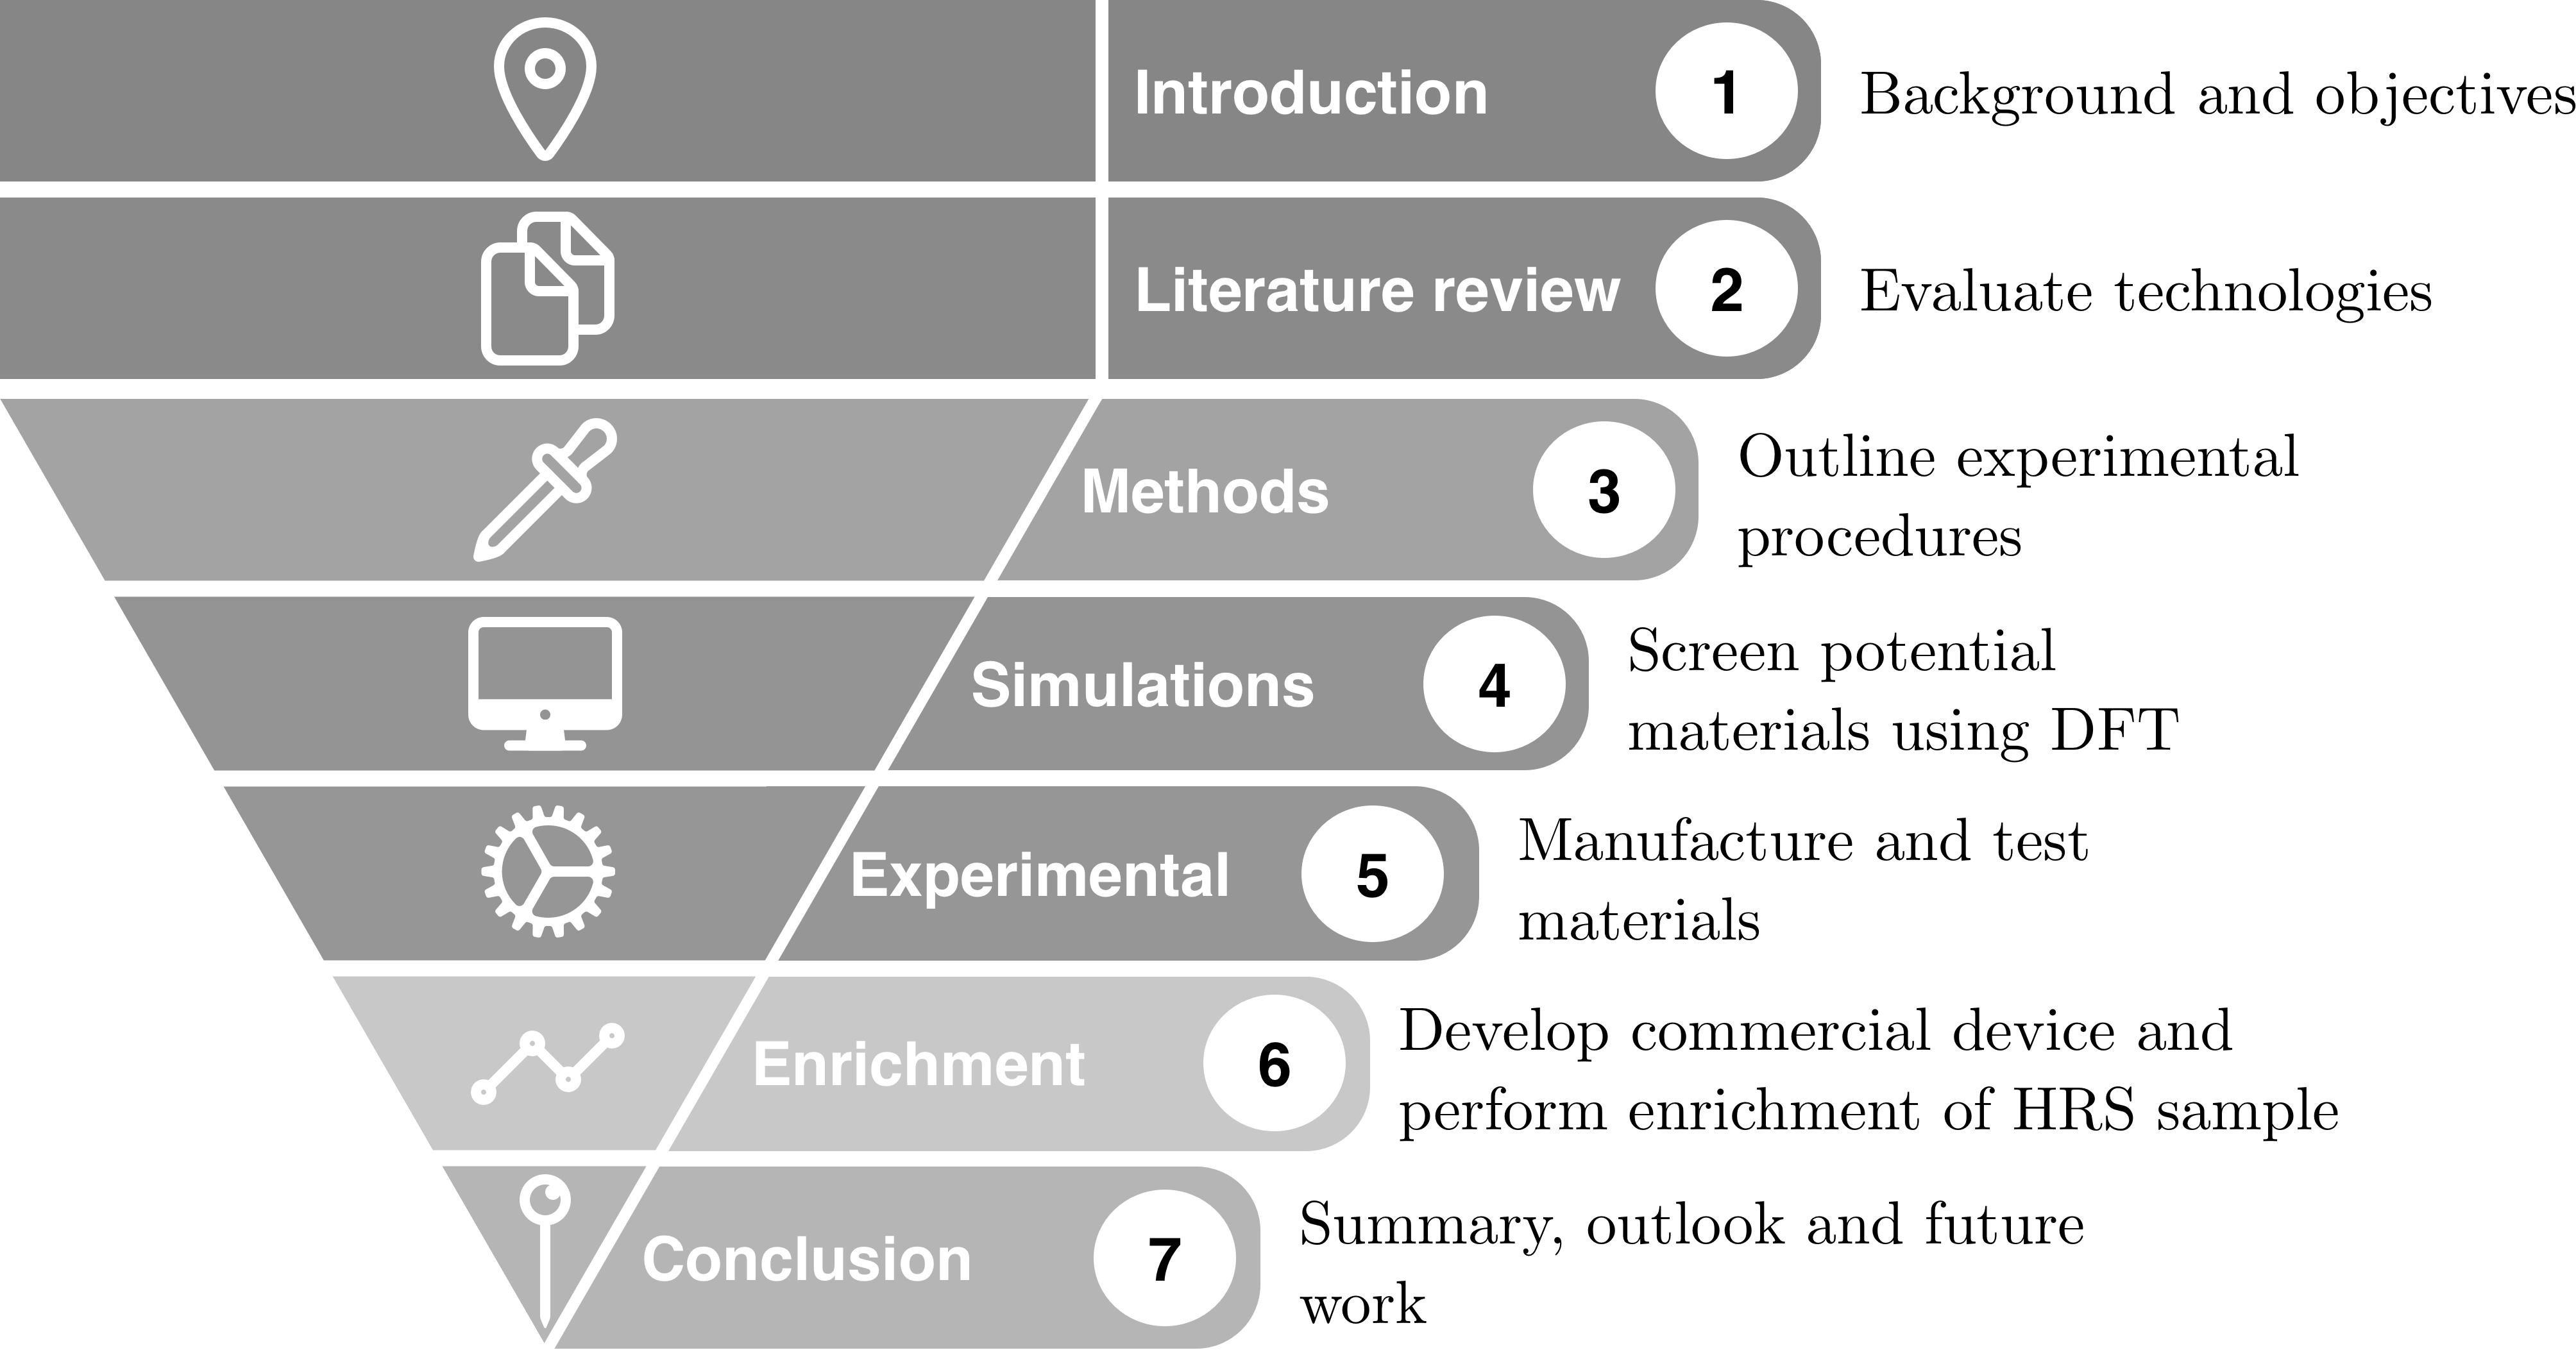
\includegraphics[width=\linewidth]{figures/funnel.png}
  \caption{Schematic presentation of the thesis structure}
  \label{funnel}
\end{figure}


\renewcommand{\bibname}{References}
\bibliographystyle{unsrtnat}
\bibliography{library.bib}


\chapter{Literature review}

\section{Fuel cell electric vehicles}
A Fuel cell electric vehicle (FCEV) refers to a vehicle which uses a solid state electrochemical device to convert chemical energy into electrical energy for motor power. The most common fuel source for FCEV's is hydrogen, where energy is produced using oxygen from air and compressed hydrogen stored on board. 

A fuel cell is made up from an electrolyte and two electrocatalysts at both the anode and cathode sides of the cell. The electrolyte separates the two electrodes and usually defines the type of fuel cell. At the anode side the fuel is oxidised as shown in equation \ref{pemfcanode}, creating a positively charged ion and an electron. The electrolyte is designed to only allow the passage of ions, and prevents the passage of electrons. The freed electron travels through a circuit, creating an electric current to provide power for it's desired use. The ions travel through the electrolyte to the cathode side of the fuel cell where they are reunited with the freed electrons, and oxygen to produce water as shown in equation \ref{pemfccathode}. The overall process for a hydrogen fuel cell is shown in equation \ref{pemfcall} and visualised in figure \ref{fig:pemfccell}

\begin{figure}[H]
    \centering
    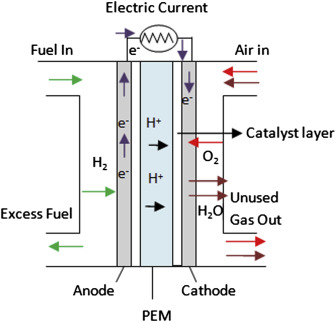
\includegraphics{figures/pemfccell.jpg}
    \caption{Schematic of a PEMFC cell \cite{Dharmalingam2019}}
    \label{fig:pemfccell}
\end{figure}

\begin{equation} \label{pemfcanode}
    H_2 \rightarrow 2H^+ + 2e^-
\end{equation}
\begin{equation} \label{pemfccathode}
    \frac{1}{2}O_2 + 2H^+ + 2e^- \rightarrow H_2 O
\end{equation}
\begin{equation} \label{pemfcall}
    H_2 + \frac{1}{2} \rightarrow H_2O
\end{equation}

While a number of fuel cell technologies can use hydrogen as a fuel source, the most suitable for FCEV's, and in particular mass production of affordable vehicles, are proton exchange membrane fuel cells (PEMFC). This is due to their high power density, low start up time, and low operating temperatures. \cite{Alaswad2016}

A PEMFC uses a proton conducting polymer membrane as an electrolyte material, typically nafion. A PEMFC cell consists of two metal bipolar plates which act to distribute the fuel and oxident within the cell, aid water management within the cell, separate individual cells in a fuel cell stack, and carry current away from the cell. \cite{Alaswad2016} A Membrane electrode assembly (MEA) which consists of the polymer membrane, two dispersed noble metal catalyst layers to enable the anode and cathode reactions, and two gas diffusion layers to ensure uniform access of fuel and oxident to the catalyst layer. Common materials for the MEA are shown in figure \ref{fig:MEA}\cite{Mehta2003}. The components are wedged between two rubber seals to ensure gas the cell is gas tight. Individual cells are combined in series to form a fuel cell stack which can provide the desired power as shown in \ref{fig:pemfcstack}

\begin{figure}[H]
    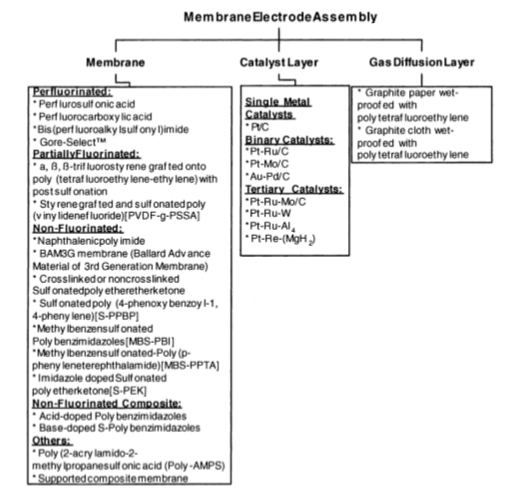
\includegraphics[scale=0.7]{figures/MEA.png}
    \caption{Classification of MEA materials \cite{Mehta2003}}
    \label{fig:MEA}
\end{figure}

\begin{figure}[H]
    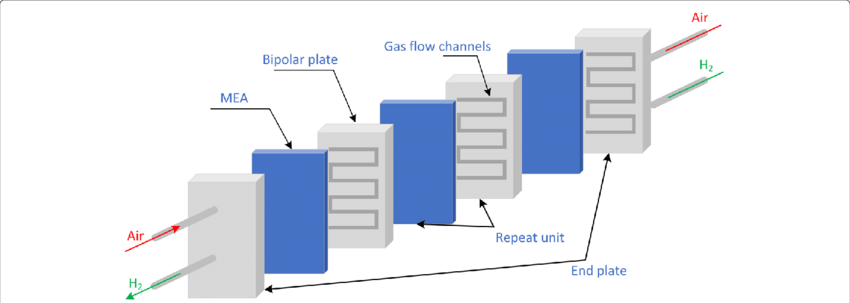
\includegraphics[scale=0.5]{figures/PEMFCstack.png}
    \caption{Schematic of a PEMFC stack \cite{Li2019}}
    \label{fig:pemfcstack}
\end{figure}

\section{Hydrogen Production}
Hydrogen production refers to a range of industrial processes for generating hydrogen. 
Since there are no natural reserves of hydrogen, it must be obtained through one of these methods. The most important factor for determining the feasibility of a hydrogen production process is the primary source of energy that is used. Currently the options for this are nuclear energy in the form of heat; renewable energy in the form of heat, electricity, light; or fossil fuels either through decomposition of the hydrocarbons present in the fuel, or through heat. 
Currently the primary sources of hydrogen are from fossil fuels: steam reforming of methane accounts for 48\% and other hydrocarbons account for 30\% of global hydrogen production; gasification of coal accounts for 18\%; and electrolysis of water accounting for the remaining 4\%. \cite{Mangold2009} Electrolysis and SMR will be discussed since these are expected to be the most dominant production methods in the future. \cite{Holladay2009}

\subsection{Hydrogen from fossil fuels and hydrocarbons}
Fossil fuels are the most dominant source of hydrogen production \cite{Mangold2009} and there are a number of processes which are commonly utilized in industry. The most popular and therefore the ones which will be discussed are steam methane reforming and hydrocarbon decomposition.

\paragraph{Steam Methane reforming} is the conventional and most economical method for producing hydrogen, and it has been predicted by the 
IEA that this trend will continue despite the emergence of other hydrogen production methods. \cite{InternationalEnergyAgencyIEA2015}
Steam methane reforming occurs through a two-step chemical process. If another hydrocarbon other than methane is being used it must first be pre-reformed into methane as shown in equation \ref{smr1}. A schematic representation of the process can be seen in figure \ref{fig:smrprocess}

\begin{figure}
    \centering
    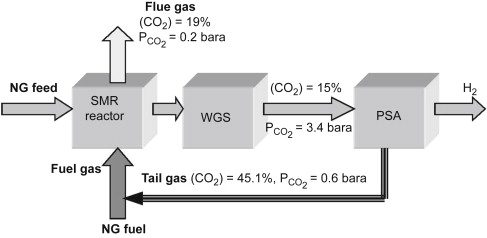
\includegraphics{figures/smrprocess.jpg}
    \caption{Simplified block diagram of a typical modern SMR plant. WGS is a water gas shift reactor. CO\textsubscript{2} concentrations are in mol.\%. \cite{Muradov2015}}
    \label{fig:smrprocess}
\end{figure}

\begin{equation} \label{smr1}
    C_n H_m + H_2 O \rightarrow nCO +(\frac{n+m}{2})H_2 
\end{equation}
\begin{equation}\label{smr2}
    CH_4 + H_2 O \rightarrow CO + 3H_2 \quad \Delta H_{298K}^o = +205 kJ/mol
\end{equation}
\begin{equation}\label{smr3}
    CO+ H_2 O \rightarrow CO_2 + H_2 \quad \Delta H_{298K}^o = -41 kJ/mol
\end{equation}

Equation \ref{smr2} takes place in a reactor operating at 700-850\textdegree C, at pressures of 3-25 bar, and in the presence of a nickel based catalyst. \cite{Muradov2015}
The result of this step is a mixture of CO and H\textsubscript{2}, commonly referred to as syngas. 
This syngas is further used as a feedstock for the reaction shown in equation \ref{smr3} known as water gas 
shift in order to produce greater hydrogen yields.  
This step is carried out in a two-step reaction. An initial high temperature stage at 350\textdegree C which converts majority of the syngas to CO\textsubscript{2} and H\textsubscript{2}, and a final low-temperature step which operates at 250\textdegree C which utilizes a catalyst with higher activity to minimise the remaining CO\textsubscript{2}. \cite{Muradov2015}
The final product will be a mixture of CO\textsubscript{2} and H\textsubscript{2}.  

A number of separation steps are used in order to prevent impurities from contaminating the 
resulting gas mixture. The traditional separation step is pressure swing adsorption (PSA) which takes 
advantage of adsorption of gaseous molecules onto a molecular sieve at high pressures. Hydrogen purities of \textasciitilde99.9\% are achievable using this method however the cost is high and typically contributes to around 
20-30\% of the total production cost. \cite{Muradov2015} The other main separation step is desulphurization which uses a 
combination of CoMo and ZnO catalysts in series at 450-550\textdegree C to remove sulphur. \cite{Muradov2015}
This step is essential to ensure sulphur is not present and to ensure catalyst 
poisoning does not occur at any point in the process. 

The cost of producting hydrogen through SMR varies but averages at around £2 per kg of hydrogen and therefore costs around £2000 per tonne of hydrogen produced. \cite{hydrogencouncil_2020}

\paragraph{Hydrocarbon decomposition} is a process by which hydrocarbon molecules are converted into solid carbon and hydrogen. \cite{Ahmed2009} This reaction is typically operated either thermally or by creating a plasma. A metallic catalyst such as nickel or iron is required. The reaction is shown in equation \ref{eq:4} \cite{Muradov2008} 

\begin{equation}\label{eq:4}
    C_x H_2x+2 \rightarrow xC + (x+1)H_2
\end{equation}

An advantage of this process is that the only feedstock is the hydrocarbon, so presuming that the feedstock is sufficiently pure this method of hydrogen production should remove the needs for further downstream processing. \cite{Ahmed2009} The main disadvantage of this method is since solid carbon is the main by-product the catalyst will be easily deactivated and will require regular maintenance to ensure carbon build up is managed. \cite{Ahmed2009}

\subsection{Hydrogen from water}

\paragraph{Electrolysis} uses an electric current to split water into hydrogen and oxygen using separate anode and cathode chambers isolated using an ion exchange membrane. The anode and cathode reactions are shown in equations \ref{electrolysis1} and \ref{electrolysis2}. The main competitive advantage of electrolysis is that reactors are modular and highly scalable, allowing hydrogen to be produced in a distributed manner. \cite{Acar2014} The main input to the process is electricity and if this electricity is produced using renewable sources then the process can be considered carbon neutral. However if a non-renewable source of energy is used the net carbon produced per mole of hydrogen would be higher than that produced by SMR. \cite{Koroneos2004}
Electrolysis is incentivised by the increasing price of natural gas and the decreasing price of electricity, which some predict will result in electrolysis becoming more economically feasible than SMR in the future. \cite{Acar2014} Currently most commercial electrolysers operate at effieicnies of around 80\% and therefore requires around 55000 kWh per tonne of hydrogen produced. The average price of industrial electricity in the UK in 2020 is around £0.13 per kWh \cite{departmentforbusinessenergyindustrialstrategy_2020} and therefore the average price of hydrogen produced through electrolysis is around £7150 per tonne. \cite{hydrogencouncil_2020}


\begin{equation}\label{electrolysis1}
Anode: \: 2H_2 O +  2e^- \rightarrow H_2 + 2OH^-
\end{equation}
\begin{equation}\label{electrolysis2}
Cathode: \: 2OH^- \rightarrow \frac{1}{2}O_2+ H_2 O + 2e^-
\end{equation}

\paragraph{Thermal decomposition of water} is the process of splitting water into hydrogen and oxygen at temperatures of 2000\textdegree C as shown in equation \ref{thermdec}. \cite{Holladay2009} The operating temperature of the reaction can be lowered under the presence of a nickel or iron based catalyst. \cite{Holladay2009} Due to the high energy demand for this production method water splitting is not a feasible method of commercial hydrogen production.

\begin{equation}\label{thermdec}
    H_2 O \rightarrow H_2 + \frac{1}{2} O_2  \quad \Delta H_{298K}^o = +286 kJ/mol
\end{equation}

\subsubsection*{Chloro Alkali process}
The chloro alkali process is an electrolysis process which involves the electrolysis of sodium chloride solutions. The process is already performed on an industrial scale in the production of chlorine and sodium hydroxide. Hydrogen is a by-product of the cathode reaction in the electrolytic cell shown in equation \label{cathode}

\begin{equation}\label{anode}
    Anode:\: 2NaCl \rightarrow Cl_2 + 2Na^+ + 2e^-
\end{equation}


\begin{equation}\label{cathode}
    Cathode:\: 2H_2O + 2e^- \rightarrow H_2 + 2NaOH
\end{equation}

\begin{equation}\label{overall}
    Overall:\: 2NaCl \rightarrow Cl_2 + 2Na^+ + 2e^-
\end{equation}

It is estimated that around 0.4 million tonnes of hydrogen per year and this could potentially contribute to annual demand. \cite{argonnenationallab_2017} The process is extremely energy intensive however, requiring 2500 kWh per tonne of NaOH produced or 99200 kWh per tonne of H\textsubscript{2} produced. \cite{doi:10.1021/ed057pA270.1} Therefore it is unlikely that this process will be used to solely produce hydrogen. As with many waste gases, producers often reuse the gas to power parts of their process, typically through consumption. It may also be the case that producers would rather find more efficient methods for performing this rather than selling their hydrogen on the open market. A recent example of this is in 2019 when a chloro alkali plant in Jordan reused their waste hydrogen in a fuel cell situated on site to power their process. \cite{doi:10.1177/0144598719839767}

\section{Hydrogen impurities in the supply chain}
The method used to manufacture hydrogen will affect which potential impurities can be present in the final product. While steps are taken in both electrolysis and SMR to ensure a pure product is produced, there is still the chance of impurities reaching the customers fuel cell. This section will explore how ISO 14687-2 impurities can enter the supply chain, and their effect on the operation of a PEMFC. A summary is shown in table \ref{impuritytbl}
\begin{table}[]
    \caption{Summary of ISO 14687-2 impurities in the supply chain and their effects on fuel cell operation adapted from \cite{Bacquart2018}}
    \resizebox{\textwidth}{!}{\begin{tabular}{@{}ccccc@{}}
    \toprule
    Impurity                               & Production sources & Contamination source                                                                                                                                                                     & Contamination barriers                                                                                                                                                            & Effect on fuel cell operation                                                                                                                                       \\ \midrule
    \multirow{2}{*}{N\textsubscript{2}}                    & SMR                & \begin{tabular}[c]{@{}c@{}}Raw material\\ PSA malfunction\end{tabular}                                                                                                                   & PSA                                                                                                                                                                               & \multirow{4}{*}{Reduced energy density of fuel}                                                                                                                     \\
                                           & Electrolysis       & \begin{tabular}[c]{@{}c@{}}Maintenance\\ Leakage\\ Air intake into water tank\end{tabular}                                                                                & \begin{tabular}[c]{@{}c@{}}Maintainance\\ PEM membrane\\ H\textsubscript{2} pressure \textgreater N\textsubscript{2} pressure supply\end{tabular}              &                                                                                                                                                                     \\
    Ar                                     & SMR                & Raw materials                                                                                                                                                                            & PSA                                                                                                                                                                               &                                                                                                                                                                     \\
    He                                     & -                  & -                                                                                                                                                                                        & -                                                                                                                                                                                 &                                                                                                                                                                     \\
    O\textsubscript{2}                                     & Electrolysis       & \begin{tabular}[c]{@{}c@{}}Generation at the anode\\ Membrane cross over\\ TSA malfunction\end{tabular}                                                              & \begin{tabular}[c]{@{}c@{}}TSA operating condition\\ Oxygen sensor\end{tabular}                                                                                                   & \begin{tabular}[c]{@{}c@{}}Potential damage to hydrogen storage\end{tabular} \\
    CO                                     & SMR                & \begin{tabular}[c]{@{}c@{}}By-product\\ Raw materials\end{tabular}                                                                                                                       & \begin{tabular}[c]{@{}c@{}}PSA\\ CO sensor on line\end{tabular}                                                                                                                   & Temporary electrocatalyst poisoning                                                                                                                                 \\
    \multirow{2}{*}{CO\textsubscript{2}}                   & SMR                & \begin{tabular}[c]{@{}c@{}}By-product\\ Raw materials\end{tabular}                                                                                                                       & PSA                                                                                                                                                                               & \multirow{2}{*}{\begin{tabular}[c]{@{}c@{}}Damage to hydrogen storage medium\\ Could cause formation of CO\end{tabular}}                                  \\
                                           & Electrolysis       & \begin{tabular}[c]{@{}c@{}}Water at anodic side\\ Air into the pure water tank\end{tabular}                                                                                              & \begin{tabular}[c]{@{}c@{}}CO\textsubscript{2} filter\\ Anodic separator tank\\ Ion exchange resin \\in closed water loop\\ PEM membrane\end{tabular} &                                                                                                                                                                     \\
    CH\textsubscript{4}                                    & SMR                & Raw material                                                                                                                                                                             & \begin{tabular}[c]{@{}c@{}}PSA\\ Methane sensor on line\end{tabular}                                                                                                              & Reduced energy density of fuel                                                                                                                                      \\
    \multirow{2}{*}{H\textsubscript{2}O}                   & SMR                & Raw material                                                                                                                                                                             & PSA                                                                                                                                                                               & \multirow{2}{*}{\begin{tabular}[c]{@{}c@{}}Ice formation during refilling\\ K+ and Na+ contamination \\ reducing cathode side conductivity\end{tabular}}            \\
                                           & Electrolysis       & \begin{tabular}[c]{@{}c@{}}Reactant\\ Through PEM membrane\\ Hydrogen output water saturated\\ TSA malfunction\end{tabular}                                                              & \begin{tabular}[c]{@{}c@{}}TSA dryer\\ Dew point monitor\\ Operating procedure\end{tabular}                                                                                       &                                                                                                                                                                     \\
    Total sulphur compounds                & SMR                & Raw material                                                                                                                                                                             & \begin{tabular}[c]{@{}c@{}}Desulfuration unit\\ Sulphur trap in reforming system \\ PSA\\ Stainless steel pipe and vessl\end{tabular}                & Permanent electrocatalyst poisoning                                                                                                                                 \\
    \multirow{2}{*}{NH\textsubscript{3}}                   & SMR                & Raw material                                                                                                                                                                             & PSA                                                                                                                                                                               & \multirow{2}{*}{Reduced ion exchange capacity}                                                                                                          \\
                                           & Electrolysis       & Water at anodic side                                                                                                                                                                     & \begin{tabular}[c]{@{}c@{}}Reverse osmosis \\ PEM membrane\end{tabular}                                                                                          &                                                                                                                                                                     \\
    Formaldehyde                           & SMR                & Raw material                                                                                                                                                                             & PSA                                                                                                                                                                               & Temporary electrocatalyst poisoning                                                                                                                                 \\
    Formic acid                            & SMR                & Raw material                                                                                                                                                                             & PSA                                                                                                                                                                               & Temporary electrocatalyst poisoning                                                                                                                                 \\
    \multirow{2}{*}{Halogenated compounds} & SMR                & Raw material                                                                                                                                                                             & \begin{tabular}[c]{@{}c@{}}Desulfuration unit\\ Chlorinated trap in reforming system \\ PSA\\ Stainless steel pipe and vessel\end{tabular}           & \multirow{2}{*}{Permanent electrocatalyst poisoning}                                                                                                                \\
                                           & Electrolysis       & \begin{tabular}[c]{@{}c@{}}Raw material contamination\end{tabular} & Reverse osmosis\\Monitoring Cl\textsubscript{2} concentration                                                                                                                                      &                                                                                                                                                                     \\ \bottomrule
    \end{tabular}}\label{impuritytbl}
    \end{table}

    
\subsection*{Water}
Water can be present from both SMR and electrolysis due to it being a main by-product of SMR reactions, and the main reactant in electrolysis. 

The PSA process used in SMR is an appropriate barrier to prevent water contaminating the end product. This is due to the molecular sieves commonly used  having a high selectivity for water. \cite{Muradov2015} When a PSA system is designed to produce an output of CO below 0.2 \textmu mol/mol, the concentration of water will be less than 0.1 \textmu mol/mol. \cite{Bacquart2018} This makes it unlikely for H\textsubscript{2}O to be present in hydrogen produced using this method.

There are three potential pathways for water to contaminate hydrogen through electrolysis. These are:
\begin{itemize}
    \item Electro-osmosis through the proton exchange membrane
    \item Hydrogen water saturated at 60\textdegree C
    \item Drier malfunction
\end{itemize}
Modern electrolysers are fitted with a drier, which is the main barrier for water vapour exiting the process with hydrogen. \cite{Bacquart2018} In the event of drier failure, most systems are fit with a dew point analyser that will trip, shutting off production until the issue can be fixed. \cite{Bacquart2018}

Water can also contaminate produced hydrogen in the chloro alkali process since, similar to electrolysis, it is present in the process. Typically the process contains a drier which ensures that a dew point of -20\textdegree C is maintained which should prevent any water in the exit stream.  

Water generally does not affect the function of a fuel cell, however; it provides a transport mechanism for water-soluble contaminants such as K\textsuperscript{+} and Na\textsuperscript{+} \cite{InternationalStandardISO14687-2:20122012} to pass through the electrolyte and have a negative long-term effect on the conductivity of the cathode side of the membrane. In addition, water may increase the risk of ice formation within vehicle fuel storage and hydrogen dispensing systems under certain conditions. 

\subsection*{Total hydrocarbon content}
The presence of hydrocarbons are most likely to result from the SMR process. Hydrocarbons are not expected to be present at all in electrolysis or chloro alkali however could potentially contaminate the system if hydrocarbons are present in any components such as compressors. Similar to water contamination through SMR, the most likely reason for hydrocarbon contamination is due to malfunction of the PSA system used to purify the product hydrogen. 

A PSA system designed to deliver hydrogen with a CO concentration $<$0.2 \textmu mol/mol should be sufficient to reduce the amount fraction of hydrocarbons to below the 5 \textmu mol/mol required by ISO 14687. \cite{Bacquart2018}

Different hydrocarbons have different effects on fuel cell performance. Generally aromatic hydrocarbons adsorb more strongly on the catalyst surface than other hydrocarbons, inhibiting access to hydrogen.\cite{InternationalStandardISO14687-2:20122012} Methane (CH\textsubscript{4}) is generally considered an inert constituent and it's main effect on fuel cell performance is  diluting the hydrogen fuel stream. \cite{InternationalStandardISO14687-2:20122012}

\subsection*{Oxygen}
In SMR processes oxygen is not used as a raw material, nor is it stable during the process conditions, readily reacting with hydrogen to produce water. In addition to this the oxygen content of the feedstock to the PSA separation stage must be below a certain level for safety reasons. Therefore oxygen contamination from hydrogen produced from SMR is unlikely. 

Oxygen is a main by-product of electrolysis, although is generated at the anode side of the electrolysis stack. Likely methods of contamination are through cross over through the PEM membrane. Due to the danger of high oxygen levels in hydrogen streams, most electrolysis systems are fit with an oxygen sensor that trips the system if the concentration of oxygen in the hydrogen stream surpasses 5 \textmu mol/mol. \cite{Bacquart2018}

Oxygen can also contaminate the exit stream in the chloro alkali process due to it's presence in ambient air. There are no safegaurds in place to prevent oxygen contaminating the hydrogen stream so it is likely that oxygen can be presence in any produced hydrogen if given the opportunity.\cite{Bacquart2018} 

Oxygen in low concentrations does not adversely affect the function of the fuel cell system; however, it may be a concern for some on-board vehicle storage systems, for example, by reaction with metal hydride storage materials. \cite{InternationalStandardISO14687-2:20122012} 

\subsection*{Helium, nitrogen and argon}
Helium is not present as a feed material in any of the discussed processes, however there is also no barrier to Helium in the exit stream and therefore any helium that enters a SMR or electrolysis process will not be removed. Despite this it is unlikely that helium will be present in a hydrocarbon feedstock, or water.

Argon is similar to helium, however it is more likely for Argon to be present in the natural gas feedstock for SMR. Unlike helium, the PSA step in SMR can act as a barrier for Argon, however this will depend on the specific molecular sieve used in the system. \cite{Bacquart2018}

Nitrogen is the most likely inert impurity to be present in fuel cell hydrogen, this is due to the abundance of nitrogen in the air which the system could be exposed to, and the frequency at which nitrogen is used as a functional gas in processes for purging chambers, actuating valves etc.

Inert constituents, such as helium (He), nitrogen (N\textsubscript{2}) and argon (Ar) do not adversely affect the function of fuel cell components or a fuel cell system. However, they dilute the hydrogen gas. N\textsubscript{2} and Ar especially can affect system operation and efficiency and can also affect the accuracy of mass metering instruments used for hydrogen dispensing. \cite{InternationalStandardISO14687-2:20122012}

\subsection*{Carbon dioxide} 
Like most other impurities which are present in SMR, CO\textsubscript{2} is likely to be removed from the SMR process at the PSA step, with most commonly used molecular sieves being able to remove carbon dioxide during normal operation. \cite{Muradov2015} 

CO\textsubscript{2} can be present in the water used for electrolysis although there are several interlocks to prevent it reaching the exit stream. Most electrolysis systems have a CO\textsubscript{2} filter on the inlet and a reverse osmosis unit to ensure the purity of the inlet water. An anodic separation tank which features an ion exchange resin in a closed water loop also acts as an additional barrier, and finally CO\textsubscript{2} has a low crossover potential through the PEM membrane and therefore is unlikely to cross into the cathode side of the system.\cite{Bacquart2018}

Carbon dioxide is not likely to be in the product stream from hydrogen produced in chloro alkali as is remains in the caustic soda lye that is produced. CO\textsubscript{2} could also be formed from oxidation of the membrane material when degraded however no quantitative assesment has been made on this. \cite{Bacquart2018}

CO\textsubscript{2} does not typically affect the function of fuel cells. However, CO\textsubscript{2} may adversely effect on board hydrogen storage systems using metal hydride alloys. With CO\textsubscript{2}, at levels higher than the specification, a reverse water gas shift reaction can occur under certain conditions in fuel cell systems to create carbon monoxide. \cite{InternationalStandardISO14687-2:20122012}

\subsection*{Carbon monoxide}
Carbon monoxide is a main byproduct of SMR which is separated from the exit gas stream through PSA. \cite{Muradov2015} If this fails SMR processes are fitted with a CO sensor to ensure the concentration in the product does not pass a certain threashold. \cite{Bacquart2018} It is unlikely for CO to be present from electrolysis.

Carbon monoxide (CO) is a severe catalyst poison that adversely effects fuel cell performance by inducing a competitive adsorption effect between itself and hydrogen on the electrocatalyst surface. The result is a temporary reduction in operating efficiency. \cite{InternationalStandardISO14687-2:20122012} Although its effect can be reversed through mitigating strategies, such as material selection of membrane electrode assembly (MEA), system design, and operating conditions, it's effect on operation is still a concern. Lower catalyst loadings are particularly susceptible to catalyst poisoning contaminants.

\subsection*{Total sulfur compounds}
Sulphur contamination is most likely to come from hydrogen produced from hydrocarbon sources. 
Since the SMR process also uses catalysts that are susceptible to poisoning from sulphur compounds all plants are fit with a desulphurisation unit upstream from the main process. \cite{Muradov2015} This is designed to reduce the concentration of sulphurous compounds to $<$50 nmol/mol. \cite{Bacquart2018}

Should the desulphurisation unit fail the catalysts used in both reforming steps will be deactivated, preventing the process from operating and will likely result in shut down of the plant. PSA also acts as a final barrier, since H\textsubscript{2}S will adsorb onto the molecular sieves more strongly than CO. \cite{Bacquart2018}

The other potential source of sulphur contamination is the potential release from any gasket materials used in the process. This can be easily prevented by ensuring only materials that do not contain sulphur are used. \cite{InternationalStandardISO14687-2:20122012}. It is unlikely that sulphur contamination will arise from electrolysis. 

Sulfur containing compounds are severe catalyst poisons that at even very low levels can cause irreversible degradation of fuel cell performance due to a permanant reaction taking place between sulphur and the platinum catalyst. The specific sulfur compounds addressed in particular are: hydrogen sulfide (H\textsubscript{2}S), carbonyl sulfide (COS), carbon disulfide(CS\textsubscript{2}), methyl mercaptan (CH\textsubscript{3}SH). \cite{InternationalStandardISO14687-2:20122012} 

\subsection*{Formaldehyde and formic acid}
Formaldehyde (HCHO) and formic acid (HCOOH) is a produced through a side reaction in SMR depending on the specific operating conditions of the process.\cite{Muradov2015} PSA is the main barrier for preventing contamination of the product. \cite{Bacquart2018}

Formaldehyde and formic acid have a similar effect on fuel cell performance as CO and are thus considered as reversible contaminants. The effect of HCHO and HCOOH on fuel cell performance can be more severe than that of CO due to slower recovery kinetics and their specifications are lower than that for CO. \cite{InternationalStandardISO14687-2:20122012} Lower catalyst loadings are particularly susceptible to catalyst poisoning contaminants.

\subsection*{Ammonia}
Hydrogen could be contaminated with ammonia through either SMR or electrolysis. Ammonia is a by-product of the reforming steps and PSA should be sufficient to remove ammoinia from the exit stream of SMR. Ammonia can also be present in water used in electrolysis however the reverse osmosis step used to purify the water before the process is normally sufficient in removing all ammonia before it is used in the process. \cite{Bacquart2018}

Ammonia (NH\textsubscript{3}) causes some irreversible fuel cell performance degradation by affecting the ion exchange capacity of the ionomer of the proton exchange membrane. \cite{InternationalStandardISO14687-2:20122012}

\subsection*{Total halogenated compounds} 
Halogenated compounds can contaminate hydrogen by entering either SMR or electrolysis through the process input, or leaking into the process at other points where they are used. Potential sources include chlor-alkali production processes, refrigerants used in processing, and cleaning agents. \cite{Bacquart2018}

In the chlor-alkali process, the presence of chlorine and hydrochloric acid in hydrogen gas could be likely since they are main feedstocks in the process. Both HCl and Cl\textsubscript{2} are highly soluble in water and are likely to leave the process in solution. Cl\textsubscript{2} and H\textsubscript{2} are also contained separatley from each other and not expected to cross contaminate. Cross contamination could occur in the event that there is not enough liquid water in the system. This would likely be detected as the system would quickly fill with hydrogen gas which is continuously monitored due to risk of explosion, shutting down the system and preventing contaminated hydrogen leaving. Therefore it is unlikely that Cl\textsubscript{ } will be present in the produced hydrogen. 
Halogenated compounds cause irreversible performance degradation similar to sulphur, reacting with the platinum electrocatalysts to form platinum-halides such as PtCl\textsubscript{4}. \cite{Dona2009} However the concentrations required to cause this damage has not been well documented in literature.

\subsection*{Other impurities}

\section{Hydrogen impurity enrichment}
'Hydrogen impurity enrichment' is a term for any technique which involves increasing the concentration of impurities within a hydrogen sample by means of removing the hydrogen matrix gas. There are two previous reports of impurity enrichment being used as a technique for hydrogen impurity 
analysis. The first report by Papadis et al at Argonne National Laboratory used a Pd/Cu \cite{Ahmed2010} coated Pd/Ag membrane for non-sulphur containing hydrogen samples and a Pd/Au coated Pd/Ag membrane for sulphur 
containing hydrogen samples to enrich impurities in a 50 bar sample. The analyte gas used contained N\textsubscript{2}, CH\textsubscript{4} and CO\textsubscript{2} at 100\textmu mol/mol and an additional 
 2 \textmu mol/mol of H\textsubscript{2}S during sulphur tests sulphur. 
The enrichment was calculated by using measured values of temperature and pressure along with the non-ideal gas law, this was represented through a 'calculated enrichment factor' as shown in equations \ref{eq:1}
and \ref{eq:2}. 

\begin{equation} \label{eq:1}
    % \frac{(\frac{P_{1,a} V_1)}{Z_{1,a} RT_{1,a}})}
    CEF_{NI} = \frac{\frac{P_{1,a} V_1}{Z_{1,a}RT_{1,a}}\frac{P_{2,a} V_2}{Z_{2,a}RT_{2,a}}-\frac{P_{1,b} V_1}{Z_{1,b}RT_{1,b}}}{\frac{P_{2,b} V_2}{Z_{2,b}RT_{2,b}}}
\end{equation}

\begin{equation}\label{eq:2}
    y_{i,a} = \frac{y_{i,b}}{CEF}
\end{equation}
The set-up was able to reach enrichment factors of around 32 for non-sulphur tests and 15 
for sulphur tests. The non-sulphur tests closely matched with the actual component concentrations, 
however in the second set of tests there was some loss of sulphur observed, most likely due to the 
formation of palladium sulphide on the surface of the membrane, or through wall catalysed reactions. 

A similar experiment was performed by National Physical Laboratory with the aim of decreasing the uncertainty 
of using such a device. \cite{Murugan2014} The non-ideal gas law method used in the previous paper \cite{Ahmed2010} 
was compared to a novel tracer enrichment method developed by NPL. \cite{Murugan2014} 
The tracer enrichment method involves spiking the hydrogen sample with a known quantity of krypton prior to 
enrichment. The enrichment factor is then calculated using the change in concentration of the krypton as 
shown in equation \ref{eq:3}.

\begin{equation} \label{eq:3}
    CEF_{Tracer} = \frac{y_{kr_b}}{y_{Kr_b}} = \frac{1}{y_{Kr_a}} \frac{A_{Kr_b}}{A_{Kr_a}} y_{Kr_{st}}
\end{equation}

The set-up was similar to the one used by Papadias et al \cite{Ahmed2010} and was used to enrich a 50 bar 10L hydrogen sample 
containing 1.5-2 \textmu mol/mol of CO, Kr, CH\textsubscript{4} and N\textsubscript{2}. Use of the tracer enrichment 
method reduced the associated uncertainty from 2.6\% to 1\%. 
Two tests were performed, with the second test resulting in membrane failure. 

When operating the hydrogen impurity enrichment device it was found that both methods should be used to 
calculate the CEF.\cite{Murugan2014, Murugan2015} While the tracer enrichment method has a lower uncertainty 
due to it being dependant on fewer variables, it is impossible to tell if a leak has occurred in the device 
due to the covariance 
phenomena. \cite{Murugan2014} Leaks in the enrichment device could occur due to thermal expansion of components due to heating 
to the required operating temperature or cracks forming in the membrane. The stability of membranes used in 
such a device will be discussed in the following section. During a leak it will be expected that the ratio of 
krypton, along with other impurities which are not naturally present in air, will remain constant, resulting 
in no change in the CEF. A leak will allow oxygen and nitrogen to enter the system and throw off the 
measurement of these two impurities. While the tracer enrichment method could still be used to calculate 
the amount fraction of other impurities, the non-ideal gas law method would have to be used to provide an 
accurate measurement for Oxygen and Nitrogen.

A device similar to the HIED is the Hydrogen Elimination Mass Spectrometer (HEMS) designed by Power + Energy USA. \cite{Bossard} 
The principle behind the HEMS is the same as the HIED, where a palladium membrane is used to selectively 
remove the hydrogen matrix gas and thus concentrate the impurities within the hydrogen sample. 
The output is directly fed into a mass spectrometer which allows in-situ measurements to be performed. 
The limit of detection specified by the manufacturer claims to be in the range of pmol/mol however there is 
no published information regarding the accuracy or uncertainty associated with the device. 
As of 2016 the device was discontinued by the manufacturer.


\subsection{Other enrichment methods}
\subsubsection{Sorbent tubes}
The use of traps and sorbent tubes to pre-concentrate impurities in gases is very common in gas analysis, 
but only two hydrogen purity analysis standards have incorporated this technique to facilitate purity analysis. 
A method for concentrating the impurities in a sample of hydrogen using a zeolite- packed chromatographic 
column has been described in a paper by Hille \cite{Hille1990a}. The method involves flowing the gas sample into the column 
using a pump and cooling the column to a temperature that allows the impurities to remain trapped whilst the 
matrix gas passes through. The sample is then transferred to GC-MS for analysis. The enrichment factor for 
this method is determined by the flowrate and amount of time that the gas is sampled into the column. 
The method was validated by analysing gas mixtures of hydrogen containing 8.7 mmol/mol of silane. 
By enriching the sample, the signal- to-noise for the same measurement was increased by a factor of 2000 
indicating that levels in the range of 4 nmol/mol of silane would easily be measured using this method 
whereas the usual limit of detection (without pre-concentration) would have been 1 \textmu mol/mol

\subsubsection{Cryo-focusing}
A method for performing pre-concentration by cryo-focusing has been detailed in ASTM WK34574 
where the device is used to concentrate the impurities in a sample of hydrogen before introducing 
the gas to a GC-MS \cite{Murugan2015} The pre-concentration method involves trapping the impurities onto a glass bead trap 
at -150\textdegree C. By increasing the temperature of the trap all of the impurities apart from water 
are transferred to a separate Tenax trap which is cooled to -170\textdegree C. 
Upon heating once again the enriched sample is introduced to the analyser. 
Very high enrichment factors can be achieved using this method by flowing a high volume of the sample 
gas through the pre-concentration device to allow capture of the impurities whilst the hydrogen is removed. 
No information was provided in the standard to indicate the accuracy or limitations of this method.

\section{Review of hydrogen selective membranes}
The term membrane is used to describe a semipermeable barrier which selectively allows certain species to 
pass through it, while preventing or inhibiting the passage of others. The driving force for gas separation 
through a membrane is the pressure and component concentration gradients across the chosen material. 
In the context of hydrogen separation, the trans-membrane pressure and hydrogen concentration gradient 
across the feed and permeate, combined with the unique properties of the chosen separation material, 
will allow hydrogen to pass through the membrane, while preventing or inhibiting the transport of impurities 
which the membrane is not selective or less selective towards. A large number of materials have been studied 
for hydrogen separation. For the purpose of this review they will be split into four broad categories based 
on their material type and separation mechanism which is related to their pore structure (dense or porous); 
these categories are shown in Table \ref{tb:1} and visualized in Figure \ref{fig:1}.

The material, its structure with regards to pore size and pore size distribution, and surface chemistry, 
all contribute to the separation mechanism for removing hydrogen from its constituent gas mixture. 
The six main membrane separation mechanisms are visualised in Figure \ref{fig:1}, with (i) – (iv) showing the 
four separation mechanisms for gases in porous media, and (V)- (Vi) showing gas separation through dense media. 
For porous materials typically a combination of these mechanisms dictates the overall separation performance 
due to imperfections in the membranes structure. All dense membranes should be dictated by the solution 
diffusion mechanism and the presence of any other mechanisms are evidence of imperfections in the membrane. 

For most porous media, the separation mechanism is dominated by Poiseuille flow or Knudsen Diffusion. 
The precise separation mechanism can be determined by calculating the ratio between the mean free path of 
the gas molecules (\textlambda) and the pore radius (r) as shown in Equation \ref{eq:6} where \texteta \ is the viscosity of the gas, 
P is the pressure, T is the temperature, M\textsubscript{w} is the molecular weight of the gas, and R is the universal gas 
constant.

\begin{figure}
    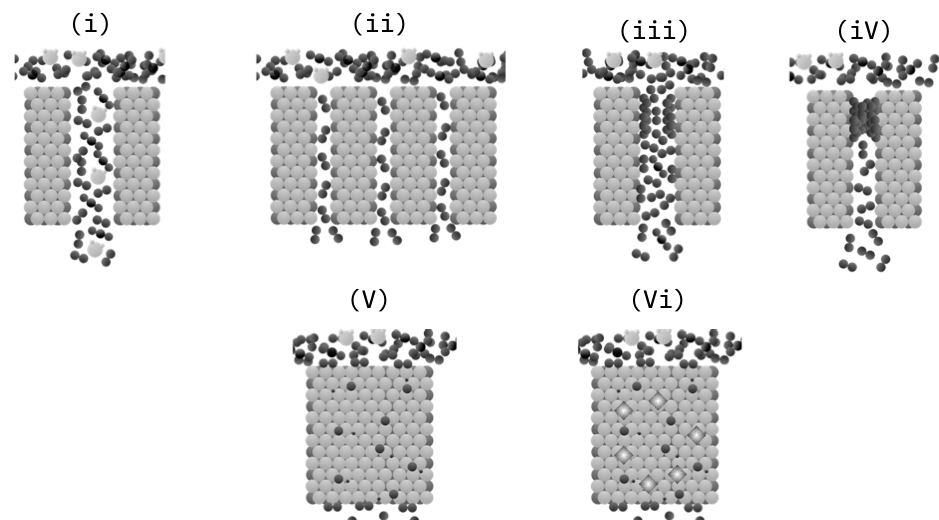
\includegraphics[width=\linewidth]{figures/septype.png}
    \caption{Illustration of the five membrane separation mechanisms (i) Poiseuille Flow/Knudsen diffusion, (ii) Molecular Sieving, (iii) Surface diffusion (iV) Capillary condensation (V) Solution diffusion (Vi) Facilitated transport}
    \label{fig:1}
  \end{figure}

\begin{equation}\label{eq:6}
    \frac{r}{\lambda} = \frac{2P}{3\eta}\sqrt{\left(\frac{2M_w}{\pi RT} \right)}
\end{equation}

This ratio determines the contribution of Knudsen and Poiseuille flow. If r/\textlambda \ $>$ 1 it would indicate 
that the main gas transport rate limiting step is due to molecule-molecule collisions indicating that 
Poiseuille flow is the dominant transport mechanism. Likewise if r/\textlambda \ $<$ 1 it indicates that 
molecule-wall collisions govern the rate limiting step showing that Knudsen diffusion is the dominant 
mechanism. If the transport is purely Knudsen diffusion the H\textsubscript{2}/CO\textsubscript{2} selectivity of 
the membrane will be equal to around 4.7. Since this value is relatively low, it has pushed researchers 
into fabricating membranes with smaller pore structures, and to modify their membranes to take advantage of 
specific surface interactions. Both of these developments allow researchers to surpass the selectivity 
achievable with purely Knudsen diffusion.

Molecular sieve materials can be classed as macroporous ($>$50nm), mesoporous (2-50nm) and microporous ($<$2nm) 
with microporous materials being the most relevant for hydrogen separation processes. These membranes are 
fabricated in such a way that the passageways are small enough that the entrance of molecules with large 
kinetic diameters is not possible. This results in higher permeation of smaller components in a gas mixture 
such as H\textsubscript{2} or He while slowing, or completely preventing the passage of bulkier molecules. This mechanism, 
while effective for some gas mixtures, may not be feasible when looking to perform separation on similar 
sized gas pairs; selectivity is often hindered by competitive adsorption between the species due to the 
surface chemistry of the material. Fabrication of these membranes can also be difficult and manufacturing 
large scale membranes with a tight enough pore size distribution to ensure molecular sieving still proves 
to be a difficult task. Common microporous materials which are able to be fabricated into molecular sieving 
membranes are zeolites, metal organic frameworks, activated carbon, and amorphous silica.

Surface diffusion and capillary condensation are similar in that the surface chemistry of the pores in the 
membrane has a large effect on the separation efficiency. Surface diffusion occurs when the walls of the pore 
either intrinsically, or following modification, provides adsorption sites for the desired gas molecule. 
The gas molecule will adsorb onto the walls resulting in faster diffusion through the pore structure than 
other gases in the mixture. Similarly, capillary condensation typically follows on from surface diffusion 
and involves the gas species condensing within the pore of the membrane, either due to stronger molecule-wall 
interactions, or a smaller pore radius. The condensation of the molecule results in further selectivity 
improvements towards this component by providing an added transport barrier to other gas species. 

Gas transport in dense media is typically harder to categorise due to the unique material chemistry present 
in each material, however all dense membranes perform separation through some variation of the solution 
diffusion mechanism. Typically, the following steps are always present in some form:
\begin{enumerate}
\item Adsorption of gas species onto the surface of the membrane 
\item Diffusion of gas species through the bulk of the membrane 
\item Desorption and diffusion of the gas species in the downstream. 
\end{enumerate}

More details will be provided on the precise features of solution diffusion in each material in the following 
sections. Facilitated transport is a sub section of solution diffusion and occurs in dense membranes which 
have a selected chemical species added into the bulk of the membrane. These materials are chosen based on the 
presence of a particular interaction with components of a gas species. These interactions are typically 
reversible reactions between the added species and the gas intended for separation and is intended to enhance 
the diffusion of the selected gas, this additive could either be fixed species (solid) or mobile (liquid). 

The most commonly reported metrics for membrane performance is the flux or permeability coefficient and 
selectivity. The flux (J) of a membrane is a measure of the amount of gas the membrane is allowing to pass 
per unit time per unit surface area and is typically used as a measure for how effective the fabricated 
membrane performs. The permeability coefficient (P) can be derived from the flux and is a quantitative 
expression which gives a specific measure of the separation properties of a material independent of 
operational and manufacturing constraints such as operating pressure and membrane thickness. 
While flux and permeability are similar and tied to each other they are both useful in their own way. 
The permeability coefficient is typically tied to the material and is useful for comparing different 
materials to each other, while the flux offers a measure on how effective a specific membrane is. 

The selectivity (\textalpha \ \textsubscript{i/j}) represents the separating ability of the membrane for a specific gas species 
(i) with respect to another gas species (j). This is common notation for porous membranes and membranes which 
are not completely selective towards one component. For membranes which are only selective towards one 
component such as dense metal and dense ceramic, the selectivity is not reported since any presence of 
another component in the exit stream is generally an indication of a manufacturing defect. 

While these values are reported for all membranes in order to allow for a direct comparison of 
performance, this is where the similarities end. The fundamental separation mechanism, manufacturing 
techniques, and unique material chemistry are often different for each material. In addition to this 
there are other important metrics for the usefulness of a membrane such as mechanical stability, lifespan, 
and chemical resistance which are more difficult to quantify. 

\begin{table}[htbp]
	\centering
	\caption{Types of hydrogen separation membrane}
	\resizebox{\textwidth}{!}{\begin{tabular}{LLLLLL}
		\hline
		\textbf{Material} & \textbf{Separation mechanism} & \textbf{Mechanical stability} & \textbf{Chemical Stability} & \textbf{Operating temperature} & \textbf{Selectivity} \\ \hline
		Polymer (Dense) & Solution diffusion, Facilitated transport &  Susceptible to Compaction \cite{Volkov2014} and Swelling \cite{Gugliuzza2015}
        & Low chemical stability, Degrades under H\textsubscript{2}S, HCl, CO\textsubscript{2}, SO\textsubscript{x} \cite{Farrauto2003} & $<100$\textsuperscript{O}C & 2.5 \cite{Nagai1995} – 960 \cite{Polotskaya2005} \\
		
		Nano-porous & Knudsen diffusion, Poiseuille flow, Capillary condensation, Surface diffusion, Molecular sieving & Brittle & Good\cite{NathanW.Ockwig2007a} & Ambient -500\textdegree C & 2.4 \cite{Lee2007} -  1000 \cite{NathanW.Ockwig2007a} (H\textsubscript{2}/N\textsubscript{2} selectivity)
        \\
        Dense Metal & Solution Diffusion & Phase transition \cite{Gao2004}
        Dependant on support \cite{Gao2004}
        Surface segregation\cite{Gao2004}
        & Negative interaction with CO, CH\textsubscript{4}, and H\textsubscript{2}O. Reacts with H\textsubscript{2}S and SO\textsubscript{x} \cite{Gao2004} & 300-600 \cite{Atsonios2015} &  $\infty$ \\ 
        Dense Ceramic & Solution Diffusion & Brittle
        Difficult to seal due to high operating temperature
        & Degrades under CO\textsubscript{2} \cite{Norby2008} & 500-1000 \cite{Norby2008}
        & $\infty$ \\ \hline
	\end{tabular}}\label{tb:1}
\end{table}

\subsection{Criteria for a hydrogen impurity enrichment material}
In order for a membrane to be suitable for hydrogen impurity enrichment material it must be able to 
increase the concentration of low-level impurities in a hydrogen sample. 
Although all past examples of hydrogen impurity enrichment have used dense membranes with an infinite 
selectivity towards hydrogen, it is theoretically possible to use a membrane which has a lower selectivity 
to perform enrichment. This would have the advantage of allowing membranes with faster flux to be used, 
greatly reducing the amount of time required for an enrichment run, while allowing cheaper materials to be 
used in place of the palladium membranes used in past studies. In order to perform this calculation, 
the following must be known:
\begin{itemize}
\item Selectivity of the membrane must be known to a high accuracy
\item Total number of moles leaving the system
\item Concentration of enriched impurities
\end{itemize}

Since the selectivity shows the ratio of substances passing through the membrane 
(i.e. H\textsubscript{2}/N\textsubscript{2} selectivity of 2 represents 2 moles of hydrogen for every 1 mole 
of nitrogen passing through 
the membrane) if both quantities are known the number of moles of impurity leaving the system through 
permeation could be easily estimated.

\begin{equation}
    n_{i_{exit}} = n_{exit_{total}}/ \alpha^{H_2 /i}    
\end{equation}

The concentration, and therefore the number of moles of impurity on the retentate side of the membrane 
could then be analysed using suitable instrumentation. These values could then be added together and 
divided by the enrichment factor in order to give the original number of moles that would be in the vessel.

\begin{equation}
    y_i=\frac{(n_{i_{ret}}+n_{i_{exit}})/n_{tot_{ret}}}{CEF} 
\end{equation}

In practice however this may not be feasible due to the low concentrations of impurities expected to be 
present in these hydrogen samples. In order for an enrichment calculation to work there must be an analysable 
concentration of impurity remaining in order to back calculate. Since the level of expected impurities in a 
hydrogen sample is so low, and the selectivity of many membranes also low, there is a high risk of either all 
impurities simply leaving the sample during the enrichment run, or only achieving a lower enrichment factor. 
Take the example of enriching a sample containing 0.2 \textmu mol/mol of CO by 100 in order to analyse its 
composition on 
a GC-MS. If the sample is a standard 10L cylinder containing 100 bar a H\textsubscript{2}/CO selectivity of 
\textasciitilde 4950000 is required to simply prevent all of the CO leaving the enrichment device, which is effectively the same as the selectivity’s seen in dense metal membranes. However, for the same sample containing 0.3 \textmu mol/mol 
of Helium a H\textsubscript{2}/He selectivity of 330 is the minimum required which is more feasible. However, both these values 
are the exact values required by the standard, in reality they would be much lower. The highest reported 
selectivity of a non-infinitely selective membrane was Liquid crystalline polyester which had a 
H\textsubscript{2}/N\textsubscript{2} 
selectivity of  2632 \cite{Weinkauf1992} which indicates that this method may be suitable for enriching some of the higher 
concentration impurities in hydrogen samples, it is not a solution for lower concentration. 
It is also unlikely that the selectivity of a membrane material will stay constant throughout its lifespan. 
Any drift in selectivity would throw off the calculation and either require regular changing of the membrane, 
driving up cost, or regular calibration to recalculate the selectivity of the membrane at a given time, which 
would be time consuming. It is however likely that infinitely selective membranes are the only feasible 
enrichment material due to their ability to enrich every impurity in hydrogen, whereas non-infinitely 
selective membranes may be applied to analysis of individual impurities, it is unlikely such a scenario 
would occur in reality which makes them a non-ideal solution. 

The common thread with all the micro-porous materials discussed here is that they are currently difficult and expensive to synthesise on a large scale, particularly in membrane form. Due to the separation mechanism of micro-porous materials they are not suitable for use in hydrogen impurity enrichment as their selectivity will not produce a viable enrichment medium. However, due to their high surface areas and ability to be modified to promote integration with specific gas species, they may find use in sensor applications for detecting the ISO-14687 impurities. There is a wealth of work on the use of many of these materials as chemical sensors however much of this work has been performed using the gases in non-hydrogen matrix gases and therefore much work is required before their true potential in this area can be realised. 

Polymer membranes have a similar issue to micro porous materials in that their selectivity 
is too low to be effective at enriching impurities in hydrogen samples. The mechanical 
strength and impurity resistance of polymer membranes also limits their use as hydrogen 
impurity enrichment mediums. While again there are some successful applications of polymers 
as sensor materials, the same issues as micro porous materials regarding lack of information 
of their effectiveness in a hydrogen matrix crops up again. It is likely that polymer 
membranes will continue to be most effective in industrial separation and will be limited in 
their use as an analytical material. 

Therefore this section will only concern itself with membranes which show permaselectivity towards hydrogen therefore making them viable as hydrogen impurity enrichment materials. This section will discuss the performance of dense metallic and dense ceramic membranes, and by comparing their reported metrics, their suitability for hydrogen impurity enrichment will be determined.

\subsubsection{Dense metallic}\label{pdreview}
Metallic membranes are comprised of dense metal or alloy sheets which allow the permeation 
of hydrogen through its constituent electrons and protons. While this is the same separation 
mechanism seen in dense polymer membranes the hydrogen selectivity is typically a lot higher 
in these systems since molecules which are not hydrogen are unable to dissociate and permeate 
through the membrane surface, giving a theoretically infinite selectivity towards hydrogen. 
The minimum requirement for a dense metal membrane for hydrogen separation is the ability to 
dissociate and permeate hydrogen. There are a number of metals which have shown varying 
degrees of suitability for hydrogen separation and these are shown in Table \ref{tb:2}.



\begin{table}[htbp]
    \centering
    \caption{Metals which show the ability for hydrogen permeation \cite{NathanW.Ockwig2007}}
    \resizebox{\textwidth}{!}{\begin{tabular}{@{}ccccc@{}}
    \toprule
    Structure            & Metal & \begin{tabular}[c]{@{}c@{}}Activation energy for \\ hydrogen permeation (kJ/mol)\end{tabular} & \begin{tabular}[c]{@{}c@{}}Heat of hydride \\ formation (kJ/mol)\end{tabular} & \begin{tabular}[c]{@{}c@{}}Hydrogen permeability at \\ 500\textdegree C (mol/ m s $pa^{1/2}$)\end{tabular} \\ \midrule
    \multirow{4}{*}{fcc} & Ni                         & 40.0                                                                                             & -6                                                                               & $7.8\times 10^{-11}$                                                                                      \\
                         & Cu                         & 38.9                                                                                             & -                                                                                & $4.9\times 10^{-12}$                                                                                      \\
                         & Pd                         & 24.0                                                                                             & 20                                                                               & $1.9\times 10^{-8}$                                                                                       \\
                         & Pt                         & 24.7                                                                                             & 26                                                                               & $2.0\times 10^{-12}$                                                                                      \\
    \multirow{4}{*}{bcc} & V                          & 5.6                                                                                              & -54                                                                              & $1.9\times 10^{-7}$                                                                                       \\
                         & Fe                         & 44.8                                                                                             & 14                                                                               & $1.8\times 10^{-10}$                                                                                      \\
                         & Nb                         & 10.2                                                                                             & -60                                                                              & $1.6\times 10^{-6}$                                                                                       \\
                         & Ta                         & 14.5                                                                                             & -78                                                                              & $1.3\times 10^{-7}$                                                                                       \\ \bottomrule
    \end{tabular}}\label{tb:2}
    \end{table}

The flux of a dense metal membrane is given by Eqn \ref{eq:7} and is a function of the metals 
permeability to hydrogen, the concentration and pressure gradient across the membrane, and 
the thickness of the dense layer. 

\begin{equation}\label{eq:7}
    J=\frac{\phi}{l} (P_{H,ret}^{0.5} - P_{H,perm}^{0.5})
\end{equation}

From the metals shown in Table \ref{tb:2} palladium and its alloys are by far the most 
popular choice due to a combination of high hydrogen permeability, favourable catalytic 
activity towards hydrogen dissociation and re-association, and aversion towards hydride 
formation compared to other metals.\cite{NathanW.Ockwig2007, Gryaznov2000, Al-Mufachi2015} 

For other metals there is often a trade-off, V, Nb and Ta exhibit higher permeability than 
palladium but are limited by their low catalytic activity for hydrogen dissociation and 
typically must be combined with another metal to compensate for this. A common strategy is 
to deposit palladium particles on both sides of membranes made from these metals to provide 
this catalytic activity. Embrittlement of pure metal membranes is also an issue, even for 
metals with a high heat of hydride formation. Embrittlement is a side effect of hydrogen 
passing through the crystal lattice. During transport a H-M phase will form which has a 
higher lattice parameter than the original crystal lattice. This change in lattice parameter 
can cause stress in the overall structure of the dense membrane layer and cause the formation 
of pin holes, cracks, and eventually membrane failure. Metals with a low heat of hydride 
formation in Table \ref{tb:2} will readily embrittle within hydrogen containing atmospheres.

This section will discuss developments in both palladium and non-palladium membranes and the issues still surrounding the technology.

As previously mentioned palladium is typically the material of choice for dense metallic 
membranes due to its combination of high stability, permeability, and catalytic activity. 
Palladium based membranes have been successfully used to provide ultrapure hydrogen for a 
number of applications including electronics, industrial gas, and fuel cell industries for a 
number of years. The main downside to the use of palladium is its high cost of around \$25 
per gram. \cite{JohnsomMattheyPreciousMetalsManagement2016} This high cost has pushed researchers into focusing on reducing the amount of 
palladium used in the membrane in order to find a more economical solution. This is done 
either by using a traditional membrane approach, whereby the thickness of the membrane layer 
is reduced as much as possible to maximise the flux while decreasing the overall amount of 
palladium used, or by alloying palladium with a cheaper metal to reduce the amount of bulk 
palladium in the manufacturing process. 

During operation of a pure palladium membrane at temperatures lower than 300\textdegree C, 
hydrogen embrittlement can occur due to the aforementioned phase transition between 
interstitial hydrogen within palladium ($\alpha$ phase) and palladium hydride ($\beta$ phase). 
The $\beta$ phase (0.4025 nm) has a lattice parameter bigger than the $\alpha$ phase 
(0.389nm). \cite{Flanagan1991}  The formation of this $\alpha$ - $\beta$ phase will cause the membrane to distort, 
become brittle, and eventually results in membrane failure when a leak occurs. \cite{Li2008b} The behaviour of hydrogen embrittlement is shown in figure \ref{alphabeta}
Aside from this pure palladium has poor chemical stability, it can be poisoned by a 
number of impurities which are commonly found in hydrogen. Some of these impurities 
simply inhibit permeation of hydrogen but do not have a permanent interaction and thus 
their effects can be mitigated by optimising the operating conditions. Others such as 
H\textsubscript{2}S and CH\textsubscript{4} are known to interact with the membrane through chemisorption and permanently 
damage the membrane through the formation of compounds with palladium, breaking the 
crystalline lattice resulting in membrane failure.  

\begin{figure}[H]
    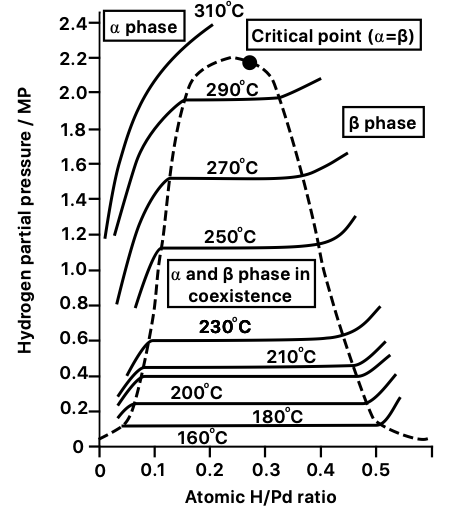
\includegraphics[width=\linewidth]{figures/alphabeta.png}
    \caption{Palladium-Hydrogen phase diagram adapted from \cite{Li2008b}}
    \label{alphabeta}
  \end{figure}


From the impurities listed in ISO 14687-2 CO, H\textsubscript{2}O, Hydrocarbons and sulphur 
containing compounds are known to have a physisorption interaction with palladium. 
Physisorption based poisoning occurs by the impurity inducing a competitive adsorption 
with hydrogen, blocking active sites for hydrogen dissociation, and hence reducing the 
active area available for hydrogen permeation.\cite{Gao2004} The ultimate effect of this is a temporary 
flux reduction which has no long lasting damage on the membrane. Compounds such as 
H\textsubscript{2}S have a more extreme effect on the membrane as 
adsorption leads to a reaction between palladium and the metal permanently changing the 
membrane composition and structure. The most commonly studied interaction is the interaction 
between palladium and H\textsubscript{2}S to form palladium sulphide. Palladium sulphide, while still
permeable to hydrogen, has an extremely low permeability, drastically reducing the efficiency 
of the membrane. Palladium sulphide also has a larger lattice constant than that of pure 
palladium which can lead to membrane failure by creating gaps in the crystal lattice 
resulting in pinholes. Some of these impurities, in particular those which only exhibit 
physisorption, can be mitigated by altering the operating conditions. It has been reported 
that the effects of CO and H\textsubscript{2}O poisoning can be completely eliminated by operating at 
temperatures above 300\textdegree C. Another example where this is shown is with H\textsubscript{2}S related poisoning. 
Since the reaction between palladium and H\textsubscript{2}S is exothermic, and produces hydrogen as a side 
product, it can be inhibited by increasing the H\textsubscript{2}:H\textsubscript{2}S ratio and increasing the temperature.  

A combination of cost, easy formation of phase transitions \cite{Flanagan1991, Li2008b} and its low tolerance for 
common impurities found in hydrogen processes limits pure palladiums use as a hydrogen 
separation material. Many of these effects however, can be completely mitigated through 
alloying palladium with another metal. By forming an alloy with a metal which has a lattice 
parameter similar to that of the $\beta$-phase the average difference between the sizes of 
the two phases is effectively decreased and thus the hydrogen embrittlement effect can be 
effectively mitigated. The effect of impurities on palladium membranes can also be partially 
mitigated by alloying with another metal and oftentimes an increase in permeability is 
reported with certain alloy compositions. 

Both binary and ternary alloys of palladium have been reported and is a mature topic in 
literature. By far the three most popular alloying compounds with palladium are silver, 
copper and gold. The current literature landscape of palladium alloy membranes are summarised 
in Table \ref{pdtable} and for the purpose of this review studies which looked at the impurity resistance, which 
is currently the most pressing issue in the field, were focused on. 

Silver is the most popular dopant for palladium membranes and forms a stable alloy with 
palladium at concentrations greater than 20wt \%, with the optimal composition occurring at 
23\%. On top of mitigating the effects of hydrogen embrittlement, a ~60\% increase in 
permeability is observed when compared to pure Pd membranes. Despite having enhanced 
permeation properties, PdAg is still susceptible to poisoning, in particular from sulphurous 
compounds which can form both Pd\textsubscript{4}S and Ag\textsubscript{5}Pd\textsubscript{10}S\textsubscript{5}. Several studies exposing PdAg membranes 
to sulphurous compounds have been performed and in most cases the membranes suffer a large 
decrease in flux, and are permanently damaged as shown by a permanent decrease in flux when 
sulphide is removed from the inlet. \cite{Mundschau2006} It has been observed that exposure to 5 \textmu mol mol\textsuperscript{-1} H\textsubscript{2}S 
in the feed stream is enough to induce Pd\textsubscript{4}S formation \cite{Mundschau2006} and therefore this composition is 
only suitable for atmospheres and applications which do not contain any sulphur. 

Copper is another widely studied binary alloy which is known to suppress hydrogen 
embrittlement. Alloying with copper also has the advantage that it reduces the cost of the 
membrane by a larger amount than most other metals and through improving the membranes 
sulphur resistance. The maximum permeability of a palladium copper membrane occurs at the 
composition Pd\textsubscript{60}Cu\textsubscript{40} and this is due to the formation of a 
bcc lattice rather than the fcc lattice commonly seen in pure palladium and most binary 
alloys. \cite{She2014} Temperature cycling has been performed on this alloy composition and it has been 
found that the bcc crystalline configuration has a higher permeability than the fcc phase. \cite{Dolan2010} 
This behaviour is due to the increased number of hcp adsorption sites which hydrogen has a 
slight preference for.\cite{Wilcox2010} Conversely the fcc structure has a higher impurity resistance 
than the bcc structure, particularly for H\textsubscript{2}S. This has been theorised to be because 
adsorption of H\textsubscript{2}S on a palladium membranes surface is largely controlled by electronic 
factors.\cite{D.T.Hughes1978a} There have been several studies reporting an increased resistance to sulphur 
poisoning by alloying palladium with copper. A Pd\textsubscript{80}Cu\textsubscript{20} 
membrane exposed to 20 \textmu mol $mol^{-1}$ of H\textsubscript{2}S for 90 hours results in a 
22\% drop in flux, performing much better than Pd\textsubscript{75}Ag\textsubscript{25} reported in the same paper which 
became impermeable after 65 hours of exposure in the same conditions.\cite{Mundschau2006} In a similar study, 
the performance of bcc and fcc alloys in response to H\textsubscript{2}S 
Pd\textsubscript{20}Cu\textsubscript{80}, Pd\textsubscript{40}Cu\textsubscript{60} and 
Pd\textsubscript{53}Cu\textsubscript{47} foils at varying temperatures was tested in 
hydrogen containing 1000 µmol $mol^{-1}$  H\textsubscript{2}S.\cite{OB2010} It was found that when the alloys were in the 
fcc phase the reduction in flux was only round 10\%, while in the bcc phase the membrane 
loses around 99\% of its permeance. The H\textsubscript{2}S concentration required to make a 
Pd\textsubscript{60}Cu\textsubscript{40} membrane completely impermeable was found to be around 300 µmol $mol^{-1}$ \cite{Kulprathipanja2005}.

PdAu alloys see a slight increase in permeability,  up to 30\% more than pure Pd, with gold 
additions up to 20\%, after which the permeability rapidly decreases. While alloying with 
gold does not improve the permeability much compared to silver or copper, gold alloys show 
greatly improved sulphur resistance. Several studies have been performed which show that PdAu 
membranes show no permanent permeability loss after exposed to ppm levels of sulphurous 
compounds implying that permeability decline is only due to H\textsubscript{2}S adsorption. 
It has been reported that a Pd\textsubscript{92}Au\textsubscript{8} membrane exposed to 
54.8 µmol $mol^{-1}$ of H\textsubscript{2}S was able to resist reaction with H\textsubscript{2}S and its permeability was 
completely recoverable. \cite{Chen2010}. When tested higher temperatures it was also found that the 
adsorption effect of H\textsubscript{2}S was reduced which is evidence that dissociative adsorption of H\textsubscript{2}S 
on metals is exothermic. \cite{Chen2010} In the original patent for palladium membranes by  McKinley \cite{DavidL.McKinley1964} 
in 1964 Pd\textsubscript{60}Au\textsubscript{40} was found to be the composition which performed best under sulphur 
containing atmospheres, losing only 9.44\% of its flux compared to the 99\% and 95\% lost by 
PdAg and PdCu membranes respectively.\cite{DavidL.McKinley1964} However under recovery the flux increased to 120\% 
of its original value while the PdCu membrane was fully recovered under the same conditions. 
This may be evidence that the Pd\textsubscript{60}Au\textsubscript{40} membrane used is not completely stable. \cite{DavidL.McKinley1964} When 
comparing the performance of PdCu and PdAu membranes under a number of gases which commonly 
result from the water gas shift reaction it was found that the PdAu resisted . \cite{RoaF.ThoenP.M.GadeS.K.WayJ.G.DeVossS.andAlptekin2009} 
It was found that from the four membranes tested, the PdAu membranes show no permeability 
loss under an atmosphere containing CO, CO\textsubscript{2} and H\textsubscript{2}O while the PdCu membranes showed 
considerable permeability loss. \cite{RoaF.ThoenP.M.GadeS.K.WayJ.G.DeVossS.andAlptekin2009} The biggest downside to alloying with gold is that 
due to its high price in recent years alloying palladium with gold drives up the price 
higher than that of a pure palladium membrane and is one of the less economic options. \cite{APMEX2016}

Other metals have been alloyed with palladium although outside of these three metals, 
studies evaluating the impurity resistance of other binary alloys are rare. The adsorption 
of CO on Pd\textsubscript{92}Y\textsubscript{8} membranes under various concentrations has been studied using TDS and XPS 
and found that CO can react with the Pd-Y allow at 623K, forming YO and solid carbon. \cite{Peng2009a}  
Bryden et al studied the poisoning resistance of nanostructured palladium-iron alloys 
compared to polycrystalline membranes of the same composition. \cite{Bryden2002} They found that 
nanostructured membranes not only display higher fluxes, but also exhibit a higher 
resistance to hydrogen sulphide poisoning. When exposed to \textasciitilde 60 µmol $mol^{-1}$, 
of H\textsubscript{2}S for 2.2 hours there was no permanent reduction in flux. 
Howard et al studied the performance of PdPt\textsubscript{20} membranes under 1000 µmol $mol^{-1}$ 
H\textsubscript{2}S at temperatures between 350\textdegree C and 450 \textdegree C. \cite{Howard2008a} 
The alloy had decent performance on the lower end of the temperature, only losing about 5\% 
of permanent permeability. At higher temperatures the membrane lost around 25\% of its 
permeability, much of this attributed to platinum segregation to the surface of the 
membrane.\cite{Howard2008a} The impurity resistance of PdPt membranes has also been studied under common 
WGS compositions which concluded that small additions of Pt (Between 5-9\%) can decrease 
the flux decline caused by WGS mixtures from 39\% for pure Pd, to anywhere between 7\%-22\%.\cite{Howard2008a}
Platinum however does not appear to be as effective at mitigating the effects of WGS mixtures 
as alloying with Au which can completely mitigate the flux decline. \cite{Gade2011} The use of Pd\textsubscript{95}Ru\textsubscript{5} 
membranes in syngas mixtures has been tested in WGS conditions and also showed good 
resistance to adsorbing compounds, losing only 6\% of their flux compared to the 
11\% lost by a pure Pd membrane under the same conditions.\cite{Ryi2011}

Ternary alloys are a newly emerging field which aims at utilizing the strengths of a binary 
alloy while mitigating its weaknesses with another component. Research in this area has 
mainly focused on ternary alloys based on copper, gold and silver however there are 
theoretically infinite combinations possible. 
A Pd\textsubscript{80}Au\textsubscript{10}Pt\textsubscript{10} membrane manufactured through 
magnetron sputtering was found to be completely resistant to H\textsubscript{2}S poisoning, 
recovering 100\% of its flux prior to exposure to impurity containing gas streams. \cite{Coulter2012} 
However after long term testing, the purity of the permeate decreased which implies that 
pinholes had started to form on the membrane surface. \cite{Coulter2012} This is most likely due to 
segregation of the individual components, destabilising the structure. This was not 
confirmed in the papers analysis however. \cite{Coulter2012} The most in depth study of PdAgAu membranes 
under H\textsubscript{2}S was performed by Braun et al, who studied the performance of Pd, 
Pd\textsubscript{90}Ag\textsubscript{10}, Pd\textsubscript{78}Ag\textsubscript{9}Au\textsubscript{13}, 
Pd\textsubscript{75}Ag\textsubscript{16}Au\textsubscript{9}, and Pd\textsubscript{91}Au\textsubscript{9}. 
While all the tested membranes saw a permanent permeability loss under 100 µmol $mol^{-1}$ 
of H\textsubscript{2}S the Pd\textsubscript{91}Au\textsubscript{9}, Pd\textsubscript{78}Ag\textsubscript{9}Au\textsubscript{13}, 
and Pd\textsubscript{75}Ag\textsubscript{16}Au\textsubscript{9} all resisted bulk corrosion 
as proven by Energy-dispersive X-ray spectroscopy (EDS), with the Pd\textsubscript{91}Au\textsubscript{9} 
sample having the highest resistance to H\textsubscript{2}S atmospheres. \cite{Braun2012, Braun2014a} While this 
study shows that ternary alloys do offer an increase in impurity resistance over pure Pd and 
PdAg membranes, the original flux values are not provided so it is difficult to see if 
there are any inherent advantages over simply using a PdAu alloy. \cite{Braun2012, Braun2014a} The Materials 
and Chemistry group at SINTEF have performed the most extensive study into ternary 
alloys, \cite{Peters2011, Peters2013} testing by far the widest range of alloys and using a combination  of X-ray 
Diffraction (XRD) and X-ray photoelectron spectroscopy to analyse the segregation behaviour 
of the ternary alloys. \cite{Peters2011, Peters2013} Through alloying PdCu alloys with a third transition metal they 
found that the addition of 1\% of a transition metal component always resulted in an increase 
in permeability, likely due to a phenomenon where the activation energy for hydrogen 
permeation decreases with increasing fcc lattice constant. \cite{He2013} In particular the addition of 
1\% Ta, 1\% Y and 14\% Ag resulted in an increase in permeability of 10, 45 and 65\% 
respectively when compared with Pd\textsubscript{73}Cu\textsubscript{27} membranes for 
Y and Ta, and Pd\textsubscript{65}Cu\textsubscript{35} membranes for Ag additions. \cite{He2013} 
In the follow up paper Pd\textsubscript{75}Ag\textsubscript{22}Au\textsubscript{3},
Pd\textsubscript{76}Ag\textsubscript{21}Mo\textsubscript{3} and Pd\textsubscript{69}Ag\textsubscript{27}Y\textsubscript{4} 
membranes were exposed to 20 µmol $mol^{-1}$ of H\textsubscript{2}S for 500 hours. 
The Pd\textsubscript{75}Ag\textsubscript{22}Au\textsubscript{3} membrane was the only 
membrane which showed no bulk sulphur formation, with the other two membrane compositions 
showing large levels of oxidation and segregation when analysed using XPS. \cite{Peters2015} The 
PdAgAu composition has been further studied by Braun et al, \cite{Braun2014a} who backed up that small 
additions of Au to PdAg membranes can reduce the membranes reactivity with sulphides and 
would be suitable for application in a hydrogen impurity enrichment device. 
Tarditi et al, have done a similar study on the impurity resistance of PdCuAu membranes. \cite{Tarditi2014} 
While XRD and EDS of this alloy showed no formation of bulk sulphides, the XPS depth 
profile showed low, but measurable levels of sulphur showing that this composition has some 
reactivity with impurities. \cite{Tarditi2014}


\eject \pdfpagewidth=16.5in \pdfpageheight=11.7in

    \begin{longtable}{@{\extracolsep{\fill}}ccccccccccccc@{}}
    \caption{Review of palladium alloys and their interactions with impurities}\label{pdtable}
    \\
    \toprule
    \multirow{2}{*}{\begin{tabular}[c]{@{}c@{}}Membrane\\composition\end{tabular}} & \multirow{2}{*}{Support} & \multicolumn{5}{c}{Susceptability to poisoning compounds}                                                                                                                   & \multirow{2}{*}{\begin{tabular}[c]{@{}c@{}}Pressure\\(bar)\end{tabular}} & \multirow{2}{*}{\begin{tabular}[c]{@{}c@{}}Permeability\\ $mol m^{-1} s^{-1} pa^{-\frac{1}{2}}$\end{tabular}} & \multirow{2}{*}{\begin{tabular}[c]{@{}c@{}}Temperature\\ \textdegree C\end{tabular}} & \multirow{2}{*}{Fabrication technique} & \multirow{2}{*}{\begin{tabular}[c]{@{}c@{}}Membrane\\ thickness (\textmu m)\end{tabular}} & \multirow{2}{*}{Ref} \\ \cmidrule(lr){3-7} 
                                          &                          & \begin{tabular}[c]{@{}c@{}}Compound\\concentration\end{tabular}                                                                    & Exposure time & \begin{tabular}[c]{@{}c@{}}Percentage\\flux drop\end{tabular} & Flux Recovery & Initial flux &                                &                                        &                                        &                                        &                                                                                    &                      \\  \midrule 
    PdAg\textsubscript{23}                                & PSS/Al\textsubscript{2}O\textsubscript{3}               & \begin{tabular}[c]{@{}c@{}}19.2\% CO\textsubscript{2}, \\ 15.4\% H\textsubscript{2}O, \\ 4\% CO, \\ 1.2\% CH\textsubscript{4}\end{tabular} & 500h          & 88.36\%               & -  & 990 $cm^3 cm^{-2} min^{-1}$       & 26                             & $2.42 \times 20^{-9}$           & 400                                    & \begin{tabular}[c]{@{}c@{}}Magnetron \\ Sputtering\end{tabular}                   & 2.2                                                                                & \cite{Peters2008a}                  \\

    PdAg\textsubscript{23}                                & PSS/Al\textsubscript{2}O\textsubscript{3}               & \begin{tabular}[c]{@{}c@{}}40.5\% CO\textsubscript{2},\\ 25\% H\textsubscript{2}O, \\ 2\% CO, \\ 2.5\% CH\textsubscript{4}\end{tabular}  & 500h          & 94.65\%               & -  & 990 $cm^3 cm^{-2} min^{-1}$       & 26                             & $2.42 \times 20^{-9}$           & 400                                    & \begin{tabular}[c]{@{}c@{}}Magnetron \\ Sputtering\end{tabular}                   & 2.2                                                                                & \cite{Peters2008a}                  \\

    PdAg\textsubscript{23}                                  & PSS/Al\textsubscript{2}O\textsubscript{3}               & \begin{tabular}[c]{@{}c@{}}60\% CO\textsubscript{2},\\ 25.5\% H\textsubscript{2}O, \\ 2\% CO, \\ 2.5\% CH\textsubscript{4}\end{tabular}  & 500h          & 94.65\%               & -  & 990 $cm^3 cm^{-2} min^{-1}$       & 26                             & $2.42 \times 20^{-9}$           & 400                                    & \begin{tabular}[c]{@{}c@{}}Magnetron \\ Sputtering\end{tabular}                   & 2.2                                                                                & \cite{Peters2008a}                  \\

    Pd                               & Self-supported               & 1000 ppm H\textsubscript{2}S & 6h          & 90\%               & -  & 14 $cm^3 cm^{-2} min^{-1}$       & 3.1                             & $1.2 \times 20^{-8}$           & 350                                    & -                   & 25                                                                                & \cite{OB2010}                  \\

    PdCu\textsubscript{53}                               & Self-supported               & 1000 ppm H\textsubscript{2}S & 6h          & 90\%               & -  & 14 $cm^3 cm^{-2} min^{-1}$       & 3.1                             & $1.3 \times 20^{-8}$           & 350                                    & -                   & 25                                                                                & \cite{OB2010}                  \\
    
    Pd                               & PSS/Al\textsubscript{2}O\textsubscript{3}               & 54.8 ppm H\textsubscript{2}S & 24h          & 93\%               & 0\%  & -       & 2.02                             & -           & 400                                    & ELP                   & 10.3                                                                                & \cite{Chen2010}                  \\

    PdAu\textsubscript{8}                               & PSS/Al\textsubscript{2}O\textsubscript{3}               & 54.8 ppm H\textsubscript{2}S & 24h          & 85\%               & 54\%  & -       & 2.02                             & -           & 400                                    & ELP/Electroplating                   & 16                                                                                & \cite{Chen2010}                  \\

    PdAg\textsubscript{23}                               & PSS               & 2 ppm H\textsubscript{2}S & 10 minutes          & 7\%               & 100\%  & 66.7 $cm^3 cm^{-2} min^{-1}$       & -                             & 1.9 $\times 10^{-8}$           & 450                                    & \begin{tabular}[c]{@{}c@{}}Magnetron \\ Sputtering\end{tabular}                   & 10                                                                                & \cite{Peters2016c}                  \\

    PdAg\textsubscript{23}                               & PSS               & 5 ppm H\textsubscript{2}S & 10 minutes          & 29\%               & 100\%  & 66.7 $cm^3 cm^{-2} min^{-1}$       & -                             & 1.9 $\times 10^{-8}$           & 450                                    & \begin{tabular}[c]{@{}c@{}}Magnetron \\ Sputtering\end{tabular}                   & 10                                                                                & \cite{Peters2016c}                  \\
    
    PdAg\textsubscript{23}                               & PSS               & 2-5-2 ppm H\textsubscript{2}S & \begin{tabular}[c]{@{}c@{}}10 minutes\\at 5ppm\end{tabular}          & 25\%               & 99.4\%  & 51.5 $cm^3 cm^{-2} min^{-1}$       & -                             & 1.9 $\times 10^{-8}$           & 450                                    & \begin{tabular}[c]{@{}c@{}}Magnetron \\ Sputtering\end{tabular}                   & 10                                                                                & \cite{Peters2016c}                  \\

    PdAg\textsubscript{23}                               & PSS               & 2-6.6-2 ppm H\textsubscript{2}S & \begin{tabular}[c]{@{}c@{}}10 minutes\\at 6.6ppm\end{tabular}          & 25\%               & 36\%  & 51.2 $cm^3 cm^{-2} min^{-1}$       & -                             & 1.9 $\times 10^{-8}$           & 450                                    & \begin{tabular}[c]{@{}c@{}}Magnetron \\ Sputtering\end{tabular}                   & 10                                                                                & \cite{Peters2016c}                  \\

    PdAg\textsubscript{23}                               & PSS               & 2-10-2 ppm H\textsubscript{2}S & \begin{tabular}[c]{@{}c@{}}10 minutes\\at 10ppm\end{tabular}          & 83\%               & 99.6\%  & 51.2 $cm^3 cm^{-2} min^{-1}$       & -                             & 1.9 $\times 10^{-8}$           & 450                                    & \begin{tabular}[c]{@{}c@{}}Magnetron \\ Sputtering\end{tabular}                   & 10                                                                                & \cite{Peters2016c}                  \\

    PdAg\textsubscript{23}                               & PSS               & 2-20-2 ppm H\textsubscript{2}S & \begin{tabular}[c]{@{}c@{}}10 minutes\\at 20ppm\end{tabular}          & 85\%               & 100\%  & 51.0 $cm^3 cm^{-2} min^{-1}$       & -                             & 1.9 $\times 10^{-8}$           & 450                                    & \begin{tabular}[c]{@{}c@{}}Magnetron \\ Sputtering\end{tabular}                   & 10                                                                                & \cite{Peters2016c}                  \\
    PdAg\textsubscript{23}                               & PSS               & 5-20-5 ppm H\textsubscript{2}S & \begin{tabular}[c]{@{}c@{}}10 minutes\\at 6.6ppm\end{tabular}          & 71\%               & 17.99\%  & 18.9 $cm^3 cm^{-2} min^{-1}$       & -                             & 1.9 $\times 10^{-8}$           & 450                                    & \begin{tabular}[c]{@{}c@{}}Magnetron \\ Sputtering\end{tabular}                   & 10                                                                                & \cite{Peters2016c}                  \\

    Pd                            & PSS/Al\textsubscript{2}O\textsubscript{3}               & \begin{tabular}[c]{@{}c@{}}111.8\% CO\textsubscript{2}, \\ 5.3\% H\textsubscript{2}O, \\ 14.2\% CO, \\ 1.7\% CH\textsubscript{4} \\ 51\% N\textsubscript{2}\end{tabular} & 48h          & 11\%               & -  & -       & 0.1                             & -           & 350                                    & ELP                   & 6.5                                                                                & \cite{Xu2016a}                  \\
    
    Pd                            & PSS/Al\textsubscript{2}O\textsubscript{3}               & \begin{tabular}[c]{@{}c@{}}11.8\% CO\textsubscript{2}, \\ 5.3\% H\textsubscript{2}O, \\ 14.2\% CO, \\ 1.7\% CH\textsubscript{4} \\ 51\% N\textsubscript{2} \\120 mg/m\textsuperscript{3} tar\end{tabular} & 24h          & 66.7\%               & -  & -       & 0.1                             & -           & 350                                    & ELP                   & 6.5                                                                                & \cite{Xu2016a}                  \\
    
    Pd                            & PSS/Al\textsubscript{2}O\textsubscript{3}               & \begin{tabular}[c]{@{}c@{}}111.8\% CO\textsubscript{2}, \\ 5.3\% H\textsubscript{2}O, \\ 14.2\% CO, \\ 1.7\% CH\textsubscript{4} \\ 51\% N\textsubscript{2} \\240 mg/m\textsuperscript{3} tar\end{tabular} & 24h          & 100\%               & -  & -       & 0.1                             & -           & 350                                    & ELP                   & 6.5                                                                                & \cite{Xu2016a}                  \\

    PdRu\textsubscript{5}                            & PSS              & \begin{tabular}[c]{@{}c@{}}11.8\% CO\textsubscript{2}, \\ 5.3\% H\textsubscript{2}O, \\ 14.2\% CO, \\ 1.7\% CH\textsubscript{4} \\ 51\% N\textsubscript{2}\end{tabular} & 48h          & 6\%               & -  & -       & 0.1                             & -           & 350                                    & ELP                   & 7.3                                                                               & \cite{Xu2016a}                  \\

    PdRu\textsubscript{5}                            & PSS             & \begin{tabular}[c]{@{}c@{}}11.8\% CO\textsubscript{2}, \\ 5.3\% H\textsubscript{2}O, \\ 14.2\% CO, \\ 1.7\% CH\textsubscript{4} \\ 51\% N\textsubscript{2} \\120 mg/m\textsuperscript{3} tar\end{tabular} & 24h          & 66.7\%               & -  & -       & 0.1                             & -           & 350                                    & ELP                   & 7.3                                                                                & \cite{Xu2016a}                  \\

    PdRu\textsubscript{5}                            & PSS             & \begin{tabular}[c]{@{}c@{}}11.8\% CO\textsubscript{2}, \\ 5.3\% H\textsubscript{2}O, \\ 14.2\% CO, \\ 1.7\% CH\textsubscript{4} \\ 51\% N\textsubscript{2} \\240 mg/m\textsuperscript{3} tar\end{tabular} & 24h          & 93\%               & -  & -       & 0.1                             & -           & 350                                    & ELP                   & 7.3                                                                                & \cite{Xu2016a}                  \\

    Pd                               & YSZ               & 50\% NH\textsubscript{3} & 75h        & 0\%               & -  & 0.056.0 $mol m^{-2} s^{-1}$       & 2-7                              & -           & 400                                    & ELP                   & 1.6                                                                                & \cite{Lundin2016}                  \\

    PdAg\textsubscript{25}                               & PSS               & 0.5\%CO & Until stable        & 80\%               & -  & -       & -                              & -           & 400                                    & -                   & 100                                                                                & \cite{Nguyen2009}                  \\

    PdAg\textsubscript{25}                               & PSS               & 0.5\%CO & Until stable        & 4\%               & -  & -       & -                              & -           & 573                                    & -                   & 100                                                                                & \cite{Nguyen2009}                  \\

    PdAg\textsubscript{25}                               & PSS               & 0.5\%CO & Until stable        & 0\%               & -  & -       & -                              & -           & 773                                    & -                   & 100                                                                                & \cite{Nguyen2009}                  \\

    PdAg\textsubscript{25}                               & PSS               & 1.5\%CO & Until stable        & 91\%               & -  & -       & -                              & -           & 400                                    & -                   & 100                                                                                & \cite{Nguyen2009}                  \\

    PdAg\textsubscript{25}                               & PSS               & 1.5\%CO & Until stable        & 7\%               & -  & -       & -                              & -           & 573                                    & -                   & 100                                                                                & \cite{Nguyen2009}                  \\

    PdAg\textsubscript{25}                               & PSS               & 1.5\%CO & Until stable        & 0\%               & -  & -       & -                              & -           & 773                                    & -                   & 100                                                                                & \cite{Nguyen2009}                  \\

    PdAg\textsubscript{25}                               & PSS               & 10\%CO & Until stable        & 98\%               & -  & -       & -                              & -           & 400                                    & -                   & 100                                                                                & \cite{Nguyen2009}                  \\

    PdAg\textsubscript{25}                               & PSS               & 10\%CO & Until stable        & 50\%               & -  & -       & -                              & -           & 573                                    & -                   & 100                                                                                & \cite{Nguyen2009}                  \\

    PdAg\textsubscript{25}                               & PSS               & 10\%CO & Until stable        & 0\%               & -  & -       & -                              & -           & 773                                    & -                   & 100                                                                                & \cite{Nguyen2009}                  \\

    PdAg\textsubscript{25}                               & PSS               & 20\%CO & Until stable        & 99.8\%               & -  & -       & -                              & -           & 400                                    & -                   & 100                                                                                & \cite{Nguyen2009}                  \\

    PdAg\textsubscript{25}                               & PSS               & 20\%CO & Until stable        & 50.5\%               & -  & -       & -                              & -           & 573                                    & -                   & 100                                                                                & \cite{Nguyen2009}                  \\

    PdAg\textsubscript{25}                               & PSS               & 20\%CO & Until stable        & 0\%               & -  & -       & -                              & -           & 773                                    & -                   & 100                                                                                & \cite{Nguyen2009}                  \\

    Pd                               & PSS               & 0.1\%H\textsubscript{2}S & 120h        & 75\%               & -  & 8.5$cm^3 cm^{-2} min^{-1}$       & -                              & 4 $\times 10^{-8}$           & 350                                    & -                   & 100                                                                                & \cite{Morreale2007}                  \\
    Pd                               & PSS               & 0.1\%H\textsubscript{2}S & 120h        & 82\%               & -  & 13.5$cm^3 cm^{-2} min^{-1}$       & -                              & 4 $\times 10^{-8}$           & 450                                    & -                   & 100                                                                                & \cite{Morreale2007}                  \\

    Pd                               & PSS               & 0.1\% H\textsubscript{2}S & 120h        & 81\%               & -  & 27.5$cm^3 cm^{-2} min^{-1}$       & -                              & 4 $\times 10^{-8}$           & 550                                    & -                   & 100                                                                                & \cite{Morreale2007}                  \\

    Pd                               & PSS               & \begin{tabular}[c]{@{}c@{}}12\% CO, \\  12\% N\textsubscript{2} \end{tabular} & Until stable       & 22\%               & -  & 8.5$cm^3 cm^{-2} min^{-1}$       & 3                              & -           & 380                                    & ELP                   & 10                                                                                & \cite{L2000}                  \\

    Pd                               & PSS               & \begin{tabular}[c]{@{}c@{}}1.6\% Steam, \\  1.6\% N\textsubscript{2} \end{tabular} & Until stable       & 17\%               & -  & 12.87$cm^3 cm^{-2} min^{-1}$       & 3                              & -           & 380                                    & ELP                   & 10                                                                                & \cite{L2000}                  \\

    Pd                            & -               & \begin{tabular}[c]{@{}c@{}}20 ppm H\textsubscript{2}S, \\  40\% N\textsubscript{2} \end{tabular} & 115h          & 71.88\%               & -  & -       & 31                             & 1.5 $\times 10^{-8}$           & 320                                    & -                   & 100                                                                                & \cite{Mundschau2006}                  \\

    PdAg\textsubscript{25}                            & -               & \begin{tabular}[c]{@{}c@{}}10 ppm H\textsubscript{2}S, \\  20\% N\textsubscript{2} \end{tabular} & 65h          & 100\%               & -  & 27.5$cm^3 cm^{-2} min^{-1}$       & 31                             & 1.4 $\times 10^{-8}$           & 320                                    & -                   & 130                                                                                & \cite{Mundschau2006}                  \\

    PdCu\textsubscript{20}                            & -               & \begin{tabular}[c]{@{}c@{}}20 ppm H\textsubscript{2}S, \\  40\% N\textsubscript{2} \end{tabular} & 90h          & 22\%               & -  & -       & 31                             & -           & 320                                    & -                   & 130                                                                                & \cite{Mundschau2006}                  \\

    PdCu\textsubscript{8}                            & PSS               & 42.7 ppm H\textsubscript{2}S & 2.5h          & 82\%               & 86.67\%  & -       & 2                             & -           & 450                                    & ELP                   & 14                                                                                & \cite{Pomerantz2009}                  \\

    PdAg\textsubscript{27}                            & -               & 4.4 ppm H\textsubscript{2}S & 48h          & 99\%               & 67\%  & 3.7$cm^3 cm^{-2} min^{-1}$       & 5.17                             & -           & 350                                    & -                   & 920                                                                                & \cite{DavidL.McKinley1964}                  \\

    PdCu\textsubscript{40}                            & -               & 4.5 ppm H\textsubscript{2}S & 72h          & 95\%               & 100\%  & 2.9$cm^3 cm^{-2} min^{-1}$       & 5.17                             & -           & 350                                    & -                   & 1030                                                                                & \cite{DavidL.McKinley1964}                  \\

    PdAu\textsubscript{40}                            & -               & 4.7 ppm H\textsubscript{2}S & 72h          & 9.4\%               & 120\%  & 0.99$cm^3 cm^{-2} min^{-1}$       & 5.17                             & -           & 350                                    & -                   & 820                                                                                & \cite{DavidL.McKinley1964}                  \\

    Pd                            & -               & 4.7 ppm H\textsubscript{2}S & 96h          & 70.1\%               & 10\%  & 1.8$cm^3 cm^{-2} min^{-1}$       & 5.17                             & -           & 350                                    & -                   & 900                                                                                & \cite{DavidL.McKinley1964}                  \\

    PdAu\textsubscript{40}                            & -               & 20.6 ppm H\textsubscript{2}S & 168h          & 56.6\%               & 120\%  & 0.99$cm^3 cm^{-2} min^{-1}$       & 5.17                             & -           & 350                                    & -                   & 790                                                                                & \cite{DavidL.McKinley1964}                  \\

    PdAu\textsubscript{40}                            & -               & 6.6\% H\textsubscript{2}S & 6h          & 99\%               & 120\%  & 0.99$cm^3 cm^{-2} min^{-1}$       & 5.17                             & -           & 350                                    & -                   & 810                                                                                & \cite{DavidL.McKinley1964}                  \\

    PdFe\textsubscript{6}                            & PSS               & 59.1 ppm H\textsubscript{2}S & 2.2h          & 75\%               & 100\%  & 8.8$cm^3 cm^{-2} min^{-1}$       & 1                             & -           & 200                                    & Electroplating                   & 10                                                                                & \cite{Bryden2002}                  \\

    PdFe\textsubscript{6}                            & PSS               & 59.1 ppm H\textsubscript{2}S & 2.2h          & 95\%               & 100\%  & 6.4$cm^3 cm^{-2} min^{-1}$       & 1                             & -           & 200                                    & Electroplating                   & 10                                                                                & \cite{Bryden2002}                  \\



    PdFe\textsubscript{5}                            & PSS               & 1\% CO & 4.2h          & 83.3\%               & -  & 5.5 $cm^3 cm^{-2} min^{-1}$       & 1                             & -           & 200                                    & Electroplating                   & 18                                                                                & \cite{Bryden2002}                  \\

    PdFe\textsubscript{5}                            & PSS               & 1\% CO & 4.2h          & 79\%               & -  & 3.9 $cm^3 cm^{-2} min^{-1}$       & 1                             & -           & 200                                    & Electroplating                   & 18                                                                                & \cite{Bryden2002}                  \\

    PdCu\textsubscript{4}                            & Accusep               & \begin{tabular}[c]{@{}c@{}} 20\% CO\textsubscript{2}, \\ 8\% CO\end{tabular} & 2h          & 17\%               & -  & 5.85 $cm^3 cm^{-2} min^{-1}$       & 1.38                             & -           & 350                                    & -                   & 7                                                                                & \cite{RoaF.ThoenP.M.GadeS.K.WayJ.G.DeVossS.andAlptekin2009}                  \\

    PdAu\textsubscript{13}                            & Accusep               & \begin{tabular}[c]{@{}c@{}} 26\% CO\textsubscript{2}, \\ 21\% H\textsubscript{2}O, \\ 2\% CO\end{tabular} & 13h          & 0\%               & -  & 35.56 $cm^3 cm^{-2} min^{-1}$       & 4.96                             & -           & 350                                    & -                   & 7                                                                                & \cite{RoaF.ThoenP.M.GadeS.K.WayJ.G.DeVossS.andAlptekin2009}                  \\

    PdCu\textsubscript{4}                            & Accusep               & \begin{tabular}[c]{@{}c@{}}50 ppm H\textsubscript{2}S \\ 26\% CO\textsubscript{2}, \\ 21\% H\textsubscript{2}O, \\ 2\% CO\end{tabular} & 2h          & 70\%               & 100\%  & 5.85 $cm^3 cm^{-2} min^{-1}$       & 4.96                             & -           & 350                                    & -                   & 7                                                                                & \cite{RoaF.ThoenP.M.GadeS.K.WayJ.G.DeVossS.andAlptekin2009}                  \\

    PdAu\textsubscript{13}                            & Accusep               & \begin{tabular}[c]{@{}c@{}}50 ppm H\textsubscript{2}S \\ 26\% CO\textsubscript{2}, \\ 21\% H\textsubscript{2}O, \\ 2\% CO\end{tabular} & 2h          & 0\%               & -  & 35.56 $cm^3 cm^{-2} min^{-1}$       & 4.96                             & -           & 350                                    & -                   & 7                                                                                & \cite{RoaF.ThoenP.M.GadeS.K.WayJ.G.DeVossS.andAlptekin2009}                  \\

    PdAu\textsubscript{10}                            & Self-supported               & \begin{tabular}[c]{@{}c@{}} 30\% CO\textsubscript{2}, \\ 19\% H\textsubscript{2}O, \\ 1\% CO\end{tabular} & 43h          & 32\%               & -  & 0.28 $mol m^{-2} s^{-1}$       & 12.7                             & -           & 400                                    & \begin{tabular}[c]{@{}c@{}}Magnetron \\ Sputtering\end{tabular}                   & -                                                                                & \cite{Coulter2012}                  \\


    PdAu\textsubscript{10}                            & Self-supported               & \begin{tabular}[c]{@{}c@{}} 30\% CO\textsubscript{2}, \\ 19\% H\textsubscript{2}O, \\ 1\% CO \\ 20ppm H\textsubscript{2}S \end{tabular} & 100h          & 70\%               & -  & 0.28 $mol m^{-2} s^{-1}$       & 12.7                             & -           & 400                                    & \begin{tabular}[c]{@{}c@{}}Magnetron \\ Sputtering\end{tabular}                   & -                                                                                & \cite{Coulter2012}                  \\

    PdAu\textsubscript{20}Pt\textsubscript{10}                            & Self-supported               & \begin{tabular}[c]{@{}c@{}} 30\% CO\textsubscript{2}, \\ 19\% H\textsubscript{2}O, \\ 1\% CO\end{tabular} & 43h          & 30\%               & -  & 0.212 $mol m^{-2} s^{-1}$       & 12.7                             & -           & 400                                    & \begin{tabular}[c]{@{}c@{}}Magnetron \\ Sputtering\end{tabular}                   & -                                                                                & \cite{Coulter2012}                  \\

    PdAu\textsubscript{20}Pt\textsubscript{10}                           & Self-supported               & \begin{tabular}[c]{@{}c@{}} 30\% CO\textsubscript{2}, \\ 19\% H\textsubscript{2}O, \\ 1\% CO \\ 20ppm H\textsubscript{2}S \end{tabular} & 100h          & 100\%               & -  & 0.28 $mol m^{-2} s^{-1}$       & 12.7                             & -           & 400                                    &                    & 33                                                                                & \cite{Coulter2012}                  \\

    PdAu\textsubscript{10.2}                           & PSS               & \begin{tabular}[c]{@{}c@{}} 30\% CO\textsubscript{2}, \\ 19\% H\textsubscript{2}O, \\ 1\% CO\end{tabular}  & 350h          & 36\%               & -  & 0.21 $mol m^{-2} s^{-1}$       & 6.27                             & -           & 400                                    & \begin{tabular}[c]{@{}c@{}}Cold \\ working\end{tabular}                   & 25                                                                                & \cite{Gade2011}                  \\

    PdAu\textsubscript{10.2}                          & PSS               & \begin{tabular}[c]{@{}c@{}} 30\% CO\textsubscript{2}, \\ 19\% H\textsubscript{2}O, \\ 1\% CO\\ 20 ppm H\textsubscript{2}S\end{tabular}  & 350h          & 72\%               & -  & 0.21 $mol m^{-2} s^{-1}$       & 6.27                             & -           & 400                                    & \begin{tabular}[c]{@{}c@{}}Cold \\ working\end{tabular}                   & 25                                                                                & \cite{Gade2011}                  \\

    PdAu\textsubscript{19}                           & PSS               & \begin{tabular}[c]{@{}c@{}} 30\% CO\textsubscript{2}, \\ 19\% H\textsubscript{2}O, \\ 1\% CO\end{tabular}  & 350h          & 0\%               & -  & 0.25 $mol m^{-2} s^{-1}$       & 6.27                             & -           & 400                                    & \begin{tabular}[c]{@{}c@{}}Cold \\ working\end{tabular}                   & 25                                                                                & \cite{Gade2011}                  \\

    PdAu\textsubscript{19}                          & PSS               & \begin{tabular}[c]{@{}c@{}} 30\% CO\textsubscript{2}, \\ 19\% H\textsubscript{2}O, \\ 1\% CO\\ 20 ppm H\textsubscript{2}S\end{tabular}  & 350h          & 0\%               & -  & 0.25 $mol m^{-2} s^{-1}$       & 6.27                             & -           & 400                                    & \begin{tabular}[c]{@{}c@{}}Cold \\ working\end{tabular}                   & 25                                                                                & \cite{Gade2011}                  \\

    PdAu\textsubscript{7}                           & PSS               & \begin{tabular}[c]{@{}c@{}} 30\% CO\textsubscript{2}, \\ 19\% H\textsubscript{2}O, \\ 1\% CO\end{tabular}  & 350h          & 32\%               & -  & 0.47 $mol m^{-2} s^{-1}$       & 6.27                             & -           & 400                                    & \begin{tabular}[c]{@{}c@{}}Cold \\ working\end{tabular}                   & 11                                                                                & \cite{Gade2011}                  \\

    PdAu\textsubscript{7}                          & PSS               & \begin{tabular}[c]{@{}c@{}} 30\% CO\textsubscript{2}, \\ 19\% H\textsubscript{2}O, \\ 1\% CO\\ 20 ppm H\textsubscript{2}S\end{tabular}  & 350h          & 68\%               & -  & 0.47 $mol m^{-2} s^{-1}$       & 6.27                             & -           & 400                                    & \begin{tabular}[c]{@{}c@{}}Cold \\ working\end{tabular}                   & 11                                                                                & \cite{Gade2011}                  \\

    PdAu\textsubscript{10.1}                           & PSS               & \begin{tabular}[c]{@{}c@{}} 30\% CO\textsubscript{2}, \\ 19\% H\textsubscript{2}O, \\ 1\% CO\end{tabular}  & 350h          & 24\%               & -  & 0.36 $mol m^{-2} s^{-1}$       & 6.27                             & -           & 400                                    & \begin{tabular}[c]{@{}c@{}}Cold \\ working\end{tabular}                   & 31                                                                                & \cite{Gade2011}                  \\

    PdAu\textsubscript{10.1}                          & PSS               & \begin{tabular}[c]{@{}c@{}} 30\% CO\textsubscript{2}, \\ 19\% H\textsubscript{2}O, \\ 1\% CO\\ 20 ppm H\textsubscript{2}S\end{tabular}  & 350h          & 62\%               & -  & 0.36 $mol m^{-2} s^{-1}$       & 6.27                             & -           & 400                                    & \begin{tabular}[c]{@{}c@{}}Cold \\ working\end{tabular}                   & 31                                                                                & \cite{Gade2011}                  \\

    Pd                         & ZrO\textsubscript{3}/PSS               &  100 ppm H\textsubscript{2}S  & 24h          & 85\%               & 16\%  & -       & -                             & 1.21$\times 10^{-8}$          & 400                                    & ELP                   & -                                                                                & \cite{Braun2014a}                  \\

    PdAg\textsubscript{10}                         & ZrO\textsubscript{3}/PSS               &  100 ppm H\textsubscript{2}S  & 24h          & 75.7\%               & 33\%  & -       & -                             & 1.65$\times 10^{-8}$          & 400                                    & ELP                   & -                                                                                & \cite{Braun2014a}                  \\

    PdAg\textsubscript{16}Au\textsubscript{9}                         & ZrO\textsubscript{3}/PSS               &  100 ppm H\textsubscript{2}S  & 24h          & 73\%               & 64.5\%  & -       & -                             & 1.18$\times 10^{-8}$          & 400                                    & ELP                   & -                                                                                & \cite{Braun2014a}                  \\

    PdAg\textsubscript{9}Au\textsubscript{13}                         & ZrO\textsubscript{3}/PSS               &  100 ppm H\textsubscript{2}S  & 24h          & 66.67\%               & 81\%  & -       & -                             & 1.34$\times 10^{-8}$          & 400                                    & ELP                   & -                                                                                & \cite{Braun2014a}                  \\

    PdAu\textsubscript{9}                         & ZrO\textsubscript{3}/PSS               &  100 ppm H\textsubscript{2}S  & 24h          & 60\%               & 80\%  & -       & -                             & 0.99$\times 10^{-8}$          & 400                                    & ELP                   & -                                                                                & \cite{Braun2014a}                  \\

    PdAg\textsubscript{23}                         & \begin{tabular}[c]{@{}c@{}}Micro channel \\ stainless steel\end{tabular}               &  \begin{tabular}[c]{@{}c@{}} 10\% N\textsubscript{2}, \\  20 ppm H\textsubscript{2}S\end{tabular}  & 1h          & 97.5\%               & 67.5\%  & 170 $cm^3 cm^{-2} min^{-1}$       & -                             & 1.3$\times 10^{-8}$          & 450                                    & \begin{tabular}[c]{@{}c@{}}Magnetron \\ Sputtering\end{tabular}                   & 2.2                                                                               & \cite{Peters2013}                  \\

    PdAg\textsubscript{22}Au\textsubscript{3}                         & \begin{tabular}[c]{@{}c@{}}Micro channel \\ stainless steel\end{tabular}               &  \begin{tabular}[c]{@{}c@{}} 10\% N\textsubscript{2}, \\  20 ppm H\textsubscript{2}S\end{tabular}  & 1h          & 87.5\%               & 80\%  & 145 $cm^3 cm^{-2} min^{-1}$       & -                             & 9.3$\times 10^{-9}$          & 450                                    & \begin{tabular}[c]{@{}c@{}}Magnetron \\ Sputtering\end{tabular}                   & 1.9                                                                               & \cite{Peters2013}                  \\

    PdAg\textsubscript{27}Y\textsubscript{4}                         & \begin{tabular}[c]{@{}c@{}}Micro channel \\ stainless steel\end{tabular}               &  \begin{tabular}[c]{@{}c@{}} 10\% N\textsubscript{2}, \\  20 ppm H\textsubscript{2}S\end{tabular}  & 1h          & 92.5\%               & 65\%  & 140 $cm^3 cm^{-2} min^{-1}$       & -                             & 1.3$\times 10^{-8}$          & 450                                    & \begin{tabular}[c]{@{}c@{}}Magnetron \\ Sputtering\end{tabular}                   & 2.4                                                                               & \cite{Peters2013}                  \\

    PdAg\textsubscript{21}Mo\textsubscript{3}                         & \begin{tabular}[c]{@{}c@{}}Micro channel \\ stainless steel\end{tabular}               &  \begin{tabular}[c]{@{}c@{}} 10\% N\textsubscript{2}, \\  20 ppm H\textsubscript{2}S\end{tabular}  & 1h          & 97.5\%               & 98\%  & 75 $cm^3 cm^{-2} min^{-1}$       & -                             & 5.8$\times 10^{-8}$          & 450                                    & \begin{tabular}[c]{@{}c@{}}Magnetron \\ Sputtering\end{tabular}                   & 2.3                                                                               & \cite{Peters2013}                  \\

    PdAg\textsubscript{11}Mo\textsubscript{4}                         & \begin{tabular}[c]{@{}c@{}}Micro channel \\ stainless steel\end{tabular}               &  \begin{tabular}[c]{@{}c@{}} 10\% N\textsubscript{2}, \\  20 ppm H\textsubscript{2}S\end{tabular}  & 1h          & 97.5\%               & 96\%  & 125 $cm^3 cm^{-2} min^{-1}$       & -                             & 8.8$\times 10^{-8}$          & 450                                    & \begin{tabular}[c]{@{}c@{}}Magnetron \\ Sputtering\end{tabular}                   & 2.2                                                                               & \cite{Peters2013}                  \\

    PdAg\textsubscript{2}Au\textsubscript{15}                         & Al\textsubscript{2}O\textsubscript{3}/PSS              &  1000 ppm H\textsubscript{2}S  & 30h          & -               & -  & -       & -                             & 1.3$\times 10^{-8}$          & 350                                    & ELP                  & -                                                                              & \cite{Braun2012}                  \\

    PdAg\textsubscript{14}Au\textsubscript{12}                         & Al\textsubscript{2}O\textsubscript{3}/PSS              &  1000 ppm H\textsubscript{2}S  & 30h          & -               & -  & -       & -                             & -          & 350                                    & ELP                  & -                                                                              & \cite{Braun2012}                  \\

    Pd                        & PSS              &  1000 ppm H\textsubscript{2}S  & 30h          & -               & -  & -       & -                             & 1.2$\times 10^{-8}$         & 350                                    & ELP                  & 25                                                                             & \cite{Braun2012}                  \\

    PdCu\textsubscript{65}                       & ZrO\textsubscript{2}/PSS              &  Varying   & Varying          & -               & -  & -       & -                             & -        & 450                                    & ELP                  & 10                                                                             & \cite{Kulprathipanja2005}                  \\

    PdCu\textsubscript{73}                       & ZrO\textsubscript{2}/PSS              &  Varying   & Varying          & -               & -  & -       & -                             & -        & 450                                    & ELP                  & 8                                                                             & \cite{Kulprathipanja2005}                  \\


    Pd                       & ZrO\textsubscript{2}/PSS              &  Varying   & Varying          & -               & -  & -       & -                             & -        & 450                                    & ELP                  & 4                                                                             & \cite{Kulprathipanja2005}                  \\

    Pd                       & ZrO\textsubscript{2}/PSS              &  Varying   & Varying          & -               & -  & -       & -                             & -        & 450                                    & ELP                  & 3                                                                             & \cite{Kulprathipanja2005}                  \\

    PdCu\textsubscript{32}                       & ZrO\textsubscript{2}/PSS              &  Varying   & Varying          & -               & -  & -       & -                             & -        & 450                                    & ELP                  & 2                                                                             & \cite{Kulprathipanja2005}                  \\

    PdCu\textsubscript{20}                       & ZrO\textsubscript{2}/PSS              &  Varying   & Varying          & -               & -  & -       & -                             & -        & 450                                    & ELP                  & 3                                                                             & \cite{Kulprathipanja2005}                  \\

    PdCu\textsubscript{40}                       & ZrO\textsubscript{2}/PSS              &  Varying   & Varying          & -               & -  & -       & -                             & -        & 450                                    & ELP                  & 15                                                                             & \cite{Kulprathipanja2005}                  \\

    PdCu\textsubscript{40}                       & ZrO\textsubscript{2}/PSS              &  Varying   & Varying          & -               & -  & -       & -                             & -        & 450                                    & Cast rolled                  & 25                                                                             & \cite{Kulprathipanja2005}                  \\

    PdPt\textsubscript{20}                       &      Self-supported         &  1000 ppm H\textsubscript{2}S   & 150h          & 50\%               & 95\%  & 1.85 $mL cm^{-2}min^{-1}$       & 6.2                             & -        & 350                                    & Mettalurgical                  & 100                                                                             & \cite{Howard2008a}                  \\

    PdPt\textsubscript{20}                       &      Self-supported         &  1000 ppm H\textsubscript{2}S   & 125h          & 80\%               & 75\%  & 2.95 $mL cm^{-2}min^{-1}$       & 6.2                             & -        & 400                                    & Mettalurgical                  & 100                                                                             & \cite{Howard2008a}                  \\

    PdPt\textsubscript{20}                       &      Self-supported         &  1000 ppm H\textsubscript{2}S   & 125h          & 25\%               & 75\%  & 3.55 $mL cm^{-2}min^{-1}$       & 6.2                             & -        & 450                                    & Mettalurgical                  & 100                                                                             & \cite{Howard2008a}                  \\

    PdY\textsubscript{8}                       &      -         &  2-26\% CO    & -          & -               & -  & -       & 0.06                             & -        & Varying                                    & -                  & -                                                                             & \cite{Peng2009a}                  \\
    
    Pd                      &      -         &  \begin{tabular}[c]{@{}c@{}}SO\textsubscript{2} \\ CS\textsubscript{2}\\H\textsubscript{2}S\end{tabular}     & -          & -               & -  & -       & 0.07 mBar                             & -        & Varying                                    & -                  & -                                                                             & \cite{Saleh1969}                  \\

    PdCu\textsubscript{20}                      &      Inconel         &  1000 ppm H\textsubscript{2}S     & -          & -               & -  & -       & -                             & -        & Varying                                    & \begin{tabular}[c]{@{}c@{}}Vacuum arc \\ welding \end{tabular}                  & 100                                                                             & \cite{Morreale2004}                  \\

    PdCu\textsubscript{40}                      &      Inconel         &  1000 ppm H\textsubscript{2}S     & -          & -               & -  & -       & -                             & -        & Varying                                    & \begin{tabular}[c]{@{}c@{}}Vacuum arc \\ welding \end{tabular}                  & 100                                                                             & \cite{Morreale2004}                  \\

    PdCu\textsubscript{47}                      &      Inconel         &  1000 ppm H\textsubscript{2}S     & -          & -               & -  & -       & -                             & -        & Varying                                    & \begin{tabular}[c]{@{}c@{}}Vacuum arc \\ welding \end{tabular}                  & 100                                                                             & \cite{Morreale2004}                  \\

    Pd                      &      PSS         &  100 ppm H\textsubscript{2}S     & 24h          & 36\%               & 80\%  & 0.0475 $mol m^{-2} s^{-1}$       & 0.5                             & 1.2 $\times10^{-8}$        & 400                                    & ELP                  & 4                                                                             & \cite{TD2014}                  \\

    PdAu\textsubscript{9}                      &      PSS         &  100 ppm H\textsubscript{2}S     & 24h          & 59\%               & 75\%  & 0.05 $mol m^{-2} s^{-1}$       & 0.5                             & 9.9 $\times10^{-9}$        & 400                                    & ELP                  & 4                                                                             & \cite{TD2014}                  \\

    PdCu\textsubscript{25}Au\textsubscript{5}                      &      PSS         &  100 ppm H\textsubscript{2}S     & 24h          & 50\%               & 74\%  & 0.01 $mol m^{-2} s^{-1}$       & 0.5                             & 1.9 $\times10^{-9}$        & 400                                    & ELP                  & 4                                                                             & \cite{TD2014}                  \\

    PdCu\textsubscript{37}Au\textsubscript{3}                      &      PSS         &  100 ppm H\textsubscript{2}S     & 24h          & 54\%               & 70\%  & 0.015 $mol m^{-2} s^{-1}$       & 0.5                             & 2.9 $\times10^{-9}$        & 400                                    & ELP                  & 4                                                                             & \cite{TD2014}                  \\

    PdAu\textsubscript{23}                      &      Accusep         &  20 ppm H\textsubscript{2}S     & 96h          & 29\%               & 97\%  & 1.4 $mol m^{-2} s^{-1}$       & 11                             & 1.55 $\times10^{-8}$        & 500                                    & ELP                  & 4.8                                                                             & \cite{Lewis2014}                  \\

    PdAu\textsubscript{20}Ag\textsubscript{13}                      &      Accusep         &  20 ppm H\textsubscript{2}S     & 96h          & 50\%               & 89\%  & 0.9 $mol m^{-2} s^{-1}$       & 11                             & 1.65 $\times10^{-8}$        & 500                                    & ELP                  & 9.3                                                                             & \cite{Lewis2014}                  \\

    \bottomrule 
    \end{longtable}

\eject \pdfpagewidth=8.3in \pdfpageheight=11.7in

\subsubsection*{Non-palladium}\label{nonpdreview}
Due to the high cost of palladium there is a particular interest to use alternative materials which still give the high selectivity intrinsic to dense metallic membranes, while reducing the cost, for example, by switching to a cheaper, non-platinum group metal. Non-palladium alloy membranes in the form of amorphous, or crystalline structures generally attract the most research interest.

Crystalline non-palladium membranes are generally based on Group IV based alloys and follow a similar philosophy to the previously discussed palladium membranes. Group IV metals are alloyed with other metals in order to improve their physical properties while maintaining the bcc structure essential for the material to transport hydrogen. Crystalline metals typically have the same advantages and disadvantages as palladium membranes. Recent research activity has focused mainly on studying how the size of the grain boundary affects the permeability of such a membrane, an area which has been mostly neglected in palladium research. \cite{NathanW.Ockwig2007a} This is likely due to the fact that many of these alloys are manufactured through cold work where the grain size can be more easily tailored than in the traditional electroless and sputtering methods used to manufacture palladium membranes. A key aspect of crystalline alloy research is the effect of nano-crystalline structures. Most research in this area has revolved around the addition of small amounts of elements to alloys based on either Zr or Hf to tailor these nano-crystalline structures and study their effects on permeability. Similarly to palladium alloys, dopants are generally chosen based on their effectiveness at suppressing hydride formation, with Zr, Mo, Ru and Rh being popular choices. \cite{Kong2011, DosSantos1998, Yukawa2002, Yukawa2002a, Yukawa2003} Alloying in this context would also likely be useful in reducing the membranes interaction with impurities through surface contamination. However this has not been touched upon much in research outside of palladium. The largest drawback to this technology is that crystalline alloys often do not show the catalytic activity necessary for dissociation of hydrogen. This requires an additional coating of palladium to be applied to the surface in order for the material to be viable for hydrogen separation. Interestingly when this was done with some commonly used industrial alloys \cite{Xu1994} it was found that they showed reasonable hydrogen permeability which further highlights the importance of catalytic dissociation of hydrogen. Crystalline membranes are also mechanically weak and still susceptible to hydrogen embrittlement through hydride formation in a similar manner to palladium membranes. \cite{NathanW.Ockwig2007a}

On the other hand amorphous metal membranes are generally seen as more attractive than crystalline membranes and are often reported to have greater mechanical strength and hydrogen solubility properties than crystalline structures due to their amorphous structure giving them a more open lattice. Unlike crystalline structures, amorphous metallic membranes can also have high catalytic activity towards hydrogen dissociation which reduces the need for an additional layer to induce this catalytic activity. This property is highly composition dependent and is typically shown by Nickel containing alloys. \cite{Hara2000} For example Zr\textsubscript{36}Ni\textsubscript{64} in its pure form due to the presence of nickel which is catalytically active for hydrogen dissociation, however when researchers started to dope the material with Ti or Hf, the catalytic properties of the material was drastically reduced and required a layer of palladium in order to induce permeability.  

Amorphous membranes still show some tendency towards hydrogen embrittlement however this is less prevalent than the crystalline alloys previously discussed. This is due to the differences in mechanisms of hydrogen embrittlement between the two classes of materials. Amorphous alloys do not show the α-β phase transition which is the main suspect of embrittlement in crystalline structures \cite{Hara2000} and the embrittlement effect is instead due to the filling of free volume within the amorphous structure. 

The main disadvantage of amorphous alloys is that given sufficient energy amorphous metallic membranes may crystallise, drastically changing their structure. This has been reported when the material is heated to high temperatures above 500\textdegree C. \cite{Hara2000} This limits the application of amorphous alloys to low-temperatures however if the material is intended to be used at 300\textdegree C, like most palladium membranes, and the material shows a high enough permeability, then this would likely not be an issue. 

Judging from the current research landscape on non-palladium membranes, the technology is still in its infancy, with most studies focusing on the fundamental properties of these alloys and with little focus on the practical applications of the technology.  Non-palladium dense metal membranes are promising due to the drastic reduction in material cost with, in many cases, an increase in permeability. Of these technologies amorphous membranes appear to be the most appealing, in particular compositions such as Zr\textsubscript{36}Ni\textsubscript{64} which require no precious metals to induce catalytic activity. This has the great advantage of reducing cost of the module and bringing dense metallic membranes, and their high associated selectivity, to a wider market by taking advantage of already established industrial production of amorphous alloys. Further practical research must be performed on these membrane compositions, in particular impurity interactions, thermal stability, and long-term stability to bring this technology to market.  

\eject \pdfpagewidth=16.5in \pdfpageheight=11.7in

    \begin{longtable}{@{\extracolsep{\fill}}C{1.7in} C{1.7in} C{1.7in} C{1.7in} C{1.7in} C{1.7in} C{1.7in} C{1.7in}@{}}
        \caption{Hydrogen permeable non-palladium metallic membranes}
        \label{nonpdtable}

        \\
    \toprule
    \begin{tabular}[c]{@{}c@{}}Membrane\\composition\end{tabular} & Structure & Catalytic coating & Feed pressure & \begin{tabular}[c]{@{}c@{}}Permeability\\ mol m\textsuperscript{2} m s\end{tabular} & \begin{tabular}[c]{@{}c@{}}Temperature\\ \textdegree C\end{tabular} & \begin{tabular}[c]{@{}c@{}}Membrane thickness\\ (\textmu m)\end{tabular} & Ref \\ \midrule
    $(Ni_{0.6}Nb_{0.4})_{70}Zr_{30}$                                                         & Amorphous &          Pd         & 7            & 1.8$\times 10^{-8}$                                      & 400                                                      & 40                                                               & \cite{YM2001} \\

    $(Ni_{0.6}Nb_{0.4})_{60}Zr_{40}$ &	Amorphous &	Pd	& 7 &	6$\times10^{-9}$  &	400 &	40	& \cite{YM2001}

    \\

    $Ni_{65}Nb_{25}Zr_{10}$	& Amorphous	& Pd	& 7 & 5 $\times10^{-9}$ & 400	& 40 & \cite{YM2001}

    \\

    $Ni_{45}Nb_{45}Zr_{10}$  & Amorphous	& Pd &	7 &	3 $\times10^{-9}$   &	400	& 40	& \cite{YM2001}

    \\

    $Ni_{60}Nb_{40}$ & Amorphous	& Pd &	7 &	2 $\times10^{-9}$   &	400	& 40	& \cite{YM2001}
    
    \\

    $Ni_{44}Nb_{43}Zr_{10}Pd_{3}$ & Amorphous	 & Pd &	7 &	1$\times10^{-9}$   &	400	& 40 & 	\cite{YM2001}
  
    \\

    $Zr_{36}Ni_{64}$ & Amorphous	& None &	1 &	1.2$\times10^{-9}$   &	350	& 30	& \cite{Hara2000a}
    
    \\

    $(Ni_{0.6}Nb_{0.4})_{45}Zr_{50}Al_{5}$ & Amorphous	 & Pd &	3 &	1.9  $\times10^{-8}$   &	400 &	50	& \cite{YM2004}
    
    \\

    $(Ni_{0.6}Nb_{0.4})_{45}Zr_{50}Co_{5} $& Amorphous	 & Pd &	3 &	2.46  $\times10^{-8}$   &	400 &	50 & \cite{YM2004}
    
    \\

    $(Ni_{0.6}Nb_{0.4})_{45}Zr_{50}Cu_{5}$ & Amorphous	 & Pd &	3 &	2.34  $\times10^{-8}$   &	400	& 50	& \cite{YM2004}
  
    \\

    $(Ni_{0.6}Nb_{0.4})_{45}Zr_{50}Pd_5$ & Amorphous	 & Pd &	3 &	1.36  $\times10^{-8}$   &	400	& 50	& \cite{YM2004}
    
    \\

    $V_{85}Ni_{15}$ & Crystalline 	& Pd &	0.8 &	5  $\times10^{-8}$   &	300	& 300-400 &	\cite{Nishimura2002}
  
    \\

    $V_{95}Ni_{15}$ & Crystalline 	& Pd &	0.1-2.0 &	4  $\times10^{-7}$   &	400	& 2000	& \cite{Ozaki2003}
    
    \\

    $V_{85}Ni_{14.91}Al_{0.09}$ & Crystalline 	& Pd &	0.1-2.0 &	4.5  $\times10^{-7}$   &	400	& 2000 & 	\cite{Ozaki2003}
  
    \\

    $V_{85}Ni_{14.1}Al_{0.9}$ & Crystalline 	& Pd &	0.1-2.0 &	4.5  $\times10^{-7}$   &	400	& 2000	& \cite{Ozaki2003}
    
    \\

   $V_{85}Ni_{12.4}Al_{2.6}$ & Crystalline 	& Pd &	0.1-2.0 &	6  $\times10^{-7}$   &	400	& 2000 &	\cite{Ozaki2003}
  
    \\

    $V_{85}Ni_{10.5}Al_{4.5}$ & Crystalline 	& Pd &	0.1-2.0 &	7  $\times10^{-7}$   &	400	& 2000 &	\cite{Ozaki2003}
    
    \\

    $V_{90}Al_{10}$ & Crystalline 	& Pd &	0.2 – 2.0 &	2  $\times10^{-7}$   &	900 &	800-2300 &	\cite{Nishimura2003}
  
    \\

    $V_{70}Al_{30}$ & Crystalline 	& Pd &	0.2 – 2.0 &	1.8  $\times10^{-9}$   &	700 &	800-2300 &	\cite{Nishimura2003}
    
    \\

    INCOLOY903 & Crystalline 	& Pd &	1 &	1.33  $\times10^{-7}$   &	430 &	200 &	\cite{Xu1994}
  
    \\

    WASPALOY & Crystalline 	& Pd &	1 &	2.99  $\times10^{-7}$   &	430	& 200 &	\cite{Xu1994}
    
    \\

    JBK-75 & Crystalline 	& Pd &	1 &	4.36  $\times10^{-7}$   &	430 &	200 &	\cite{Xu1994}
  
    \\

    GH85A & Crystalline 	& Pd &	1 &	2.73  $\times10^{-7}$   &	430	& 200 &	\cite{Xu1994}
    
    \\

    INCOLOY907 & Crystalline 	& Pd &	1 &	9.67  $\times10^{-8}$  &	430 &	200 &	\cite{Xu1994}
  
    \\

    INCONEL718 & Crystalline 	& Pd &	1 &	2.22  $\times10^{-7}$   &	430	& 200 &	\cite{Xu1994}
    
    \\

    GH761 & Crystalline 	& Pd &	1 &	1.5  $\times10^{-7}$   &	430	& 200 &	\cite{Xu1994}
  
    \\

    $Nb_{20}Zr_{35}Ni_{35}$ & Crystalline 	& Pd &	1 &	2.73  $\times10^{-8}$   &	400 &	500-700 &	\cite{Takano2004}
    
    \\

    $Nb_{10}Zr_{45}Ni_{45}$ & Crystalline 	& Pd &	1 &	2.5  $\times10^{-8}$   &	400 &	500-700 &	\cite{Takano2004}
  
    \\
    
    $Nb_{29}Ti_{31}Ni_{40}$ & Crystalline 	& Pd &	2 &	7  $\times10^{-9}$   &	400 &	550-750 &	\cite{Hashi2005}
    
    \\

    Nb17Ti42Ni41 & Crystalline 	& Pd &	2 &	0.6  $\times10^{-8}$   &	400 &	550-750 &	\cite{Hashi2005}
  
    \\

    Nb10Ti50Ni40 & Crystalline 	& Pd &	2 &	4.5  $\times10^{-9}$   &	400 &	550-750 &	\cite{Hashi2005}
    
    \\

    Nb39Ti31Ni30 & Crystalline 	& Pd &	2 &	2.0  $\times10^{-8}$   &	400 &	550-750 &	\cite{Hashi2005}
  
    \\

    Nb28Ti42Ni30 & Crystalline 	& Pd &	2 &	1  $\times10^{-8}$   &	400 &	550-750 &	\cite{Hashi2005}
    
    \\

    Nb21Ti50Ni29 & Crystalline 	& Pd &	2 &	1  $\times10^{-8}$   &	400	& 550-750 &	\cite{Hashi2005}
  
    \\

    $Ta_{95}W_{5}$ & Crystalline &	None	& 1.4 &	52 $mol m^{-2} s^{-1}$ &	500 &	650 &	\cite{Yukawa2011}
    
    \\ \bottomrule
    \end{longtable}
    \eject \pdfpagewidth=8.3in \pdfpageheight=11.7in


\subsubsection{Dense Ceramic}
Dense ceramic membranes operate in a similar manner to metallic membranes, with the key 
difference being that they are made from ion conducting ceramics rather than metals. 
Dense ceramic membranes have a selectivity comparable to dense metal membranes since they 
only allow hydrogen to permeate, however at a lower cost than Pd-based membranes. 
Unlike dense metallic membranes, most ion conducting materials claim to be intrinsically 
inert to common hydrogen impurities and hence are stable in CO, CO\textsubscript{2} 
and H\textsubscript{2}S containing atmospheres. \cite{NathanW.Ockwig2007a} The major drawback to ion conducting ceramic
membranes is that generally high temperatures are required to achieve any form of 
H\textsubscript{2} flux. While palladium membranes can achieve a high flux at temperatures 
between 300-400\textdegree C, most Perovskite membranes require temperatures between 700-900\textdegree 
C and generally only achieve a hydrogen permeability $<$10\% compared to a palladium 
membrane of the same thickness.  

The hydrogen separation process in a dense ceramic membrane is near identical to that which 
occurs in a dense metal membrane with the main driving forces being the pressure and 
concentration gradients. This is primarily controlled by the catalytic surface effects and 
bulk diffusion rather than thickness due to ceramic materials intrinsically low catalytic 
activity for such a process. For practical purposes both sides of the membrane should have 
sufficient catalytic activity to dissociate hydrogen atoms and the bulk should have high 
enough proton and electron conductivities to ensure a reasonably high flux can be achieved. 
More information on the precise mechanism behind proton conducting membranes can be found in 
the following reviews \cite{Tao2015, Phair2006}. The bulk diffusion of a dense ceramic membrane can be 
described through the Wagner equation written as Eq \ref{eq:5}

\begin{equation} \label{eq:5}
    J_{H_2} = \frac{RT}{4F^2L} \frac{\theta_H \theta_e}{\theta_H + \theta_e} ln \left(\frac{P_{H_2}'}{P_{H_2}''} \right)
\end{equation}
\renewcommand{\bibname}{References}

Dense ceramic membranes can be split into two broad categories; single phase ceramic 
membranes are composed of a single material which has the ability to conduct both protons 
and electrons, and multi-phase ceramic membranes which are normally composed of two or more 
phases which when combined show proton and electron conductivity. The most common type of 
multi-phase ceramic membranes is known as ‘cermet’ which combines a proton conducting ceramic 
and a metal, such as palladium or nickel, as the electron conducting phase.

Single phase ceramic membranes must be given proton conductivity by doping a single phase 
ceramic material (typically perovskite) in order to create a proton hole within the material. 
This combined with catalytic dissociation of hydrogen  on the surface allows uptake of a 
certain number of protons, which then diffuse through the material using the proton holes 
within the material. \cite{Tao2015, Phair2006}

Extensive efforts have been placed into developing proton-electron conducting ceramic 
materials for hydrogen separation however there are still many technical hurdles which must 
be overcome before the technology can be applied on a useful scale. The main problem holding 
back the technology is the incredibly low flux values reported despite operating at such high 
temperatures. Until this is solved there will be no point in using the technology over 
faster porous materials, or even dense metal membranes which offer the same selectivity’s, 
at much faster permeation rates. This stems back to a lack of understanding behind the 
surface kinetics of hydrogen dissociation (which is also an issue for non-palladium dense 
membranes). Despite claims that ceramic membranes are inert to impurities there is 
contradictory evidence showing that the materials cannot withstand acidic conditions and 
degrade under atmospheres containing CO\textsubscript{2} and H\textsuperscript{2}S. 
Finally, since such high temperatures are 
required there will be difficulties forming a hermetic seal with ceramic membranes which can 
withstand the high temperature environments. This is already an issue with ceramic supported 
metallic membranes which operate at much more mild conditions. 

From this it can be concluded that dense ceramic membranes for hydrogen separation are still 
at a research level and a better understanding of the material science behind the surface 
interactions with hydrogen and other gases, along with research into new classes of ceramics 
which can either permeate hydrogen at faster rates, at lower temperatures, or both are key 
to bringing this technology to market. 


\eject \pdfpagewidth=16.5in \pdfpageheight=11.7in


    \begin{longtable}{@{}C{5cm} C{2cm} C{4cm} ccc C{6cm} C{5cm} C{0.5cm} @{}}
        \caption{Hydrogen permeable ceramic and cermet membranes which show resistance to common hydrogen impurities}
        \label{ceramtable}
    \\
    \toprule
    Material & Class    & Feed & Temperature \textdegree C & Flux   & \begin{tabular}[c]{@{}c@{}}Thickness\\ (\textmu m)\end{tabular} & Stability & Notes & Ref \\ \midrule


    $SrCe_{0.75}Zr_{0.2}Tm_{0.05}O_{3-\alpha}$
    & Perovskite    
    & 100 $mL min^{-1}$ 50\% H\textsubscript{2} + He
    & 900	
    & 0.042 $mL cm^{-2} min^{-1} $
    & 1200 
    & -	
    & -	
    & \cite{Yuan2010}

\\ $Nd_{5.5}WO_{12-\alpha}$
	& Lanthanide tungstate
	& 80\% He + 20 \% H\textsubscript{2}
	& 1000
    & 0	
    & 900
	& Stable under 115 ppm H\textsubscript{2}S, 4.43\% CO\textsubscript{2}, 2.12\% CO
    & No flux due to dry conditions	
    & \cite{Escolastico2011}

\\ $La_{5.5}WO_{11.25}$
	& Lanthanide tungstate
	& 80\% He + 20 \% H\textsubscript{2}
	& 1000
	& $<0.005 mL min^{-1} cm^{-2}$
	& 900
	& Stable in 15\% CO\textsubscript{2} for 3 days
	& Requires humidification for faster permeation
	& \cite{Escolastico2013}

\\$Nd_6 Wo_{12}$
	& Lanthanide tungstate
	& He + H\textsubscript{2}
	& 1000
	& 0.012 $mL min^{-1} cm^{-2}$
	& 510
	& Stable in CO\textsubscript{2} and CH4 after 3 days
	& Humidified atmosphere
	& \cite{Escolastico2009}

\\ $La_{5.5} W_{0.8} Re_{0.2} O_{11.25-\alpha}$
	& Lanthanide tungstate
	& 2.5\% H\textsubscript{2}, 2.5\% H\textsubscript{2}O, H\textsubscript{2} balance
	& 1000
	& 0.095$ mL min^{-1} cm^{-2}$
	& 760
	& Stable in 5\% CO\textsubscript{2} 1000 ppm COS 100 ppm HCN 46\% CO 46\% H\textsubscript{2} at 35 bar
	& Humidified atmosphere
	& \cite{Escolastico2013a}

\\ $(La_{5/6} Nd_{1/6})_{5.5} WO_{12-\alpha}$	
    & Lanthanide tungstate
	& 80\% He + 20 \%H\textsubscript{2}
	& 1000
	& 0.005$ mL min^{-1} cm^{-2}$
	& 900
	& Stable in 15\% CO\textsubscript{2} for 3 days
    & Requires humidification	
    & \cite{Escolastico2012}

\\ $La_{27} Mo_{1.5} W_{3.5} O_{55.5}$
	& Lanthanide tungstate
	& 10\% H\textsubscript{2} 90\% He
	& 700
	& $ 0.78 \times 10^{−4} mL min^{-1} cm^{-2}$
	& 650
    & -
    & -	
    & \cite{Vollestad2014}

    \\ $La_{27} Mo_{1.5} W_{3.5} O_{55.5}$
	& Lanthanide tungstate
	& 10\% H\textsubscript{2} 90\% He
	& 700
	& $ 0.78 \times 10^{−4} mL min^{-1} cm^{-2}$
	& 650
    & -
    & -	
    & \cite{Vollestad2014}

\\ $Nd_{5.5} W_{0.5} Mo_{0.5} O_{11.25-\alpha}$
	& Lanthanide tungstate
	& 50\% H\textsubscript{2}, 50\% He
	& 1000
	& 0.235 $mL cm^{-2} min^{-1}$
	& 900
    & Stable in environments containing 330 ppm H\textsubscript{2}S and 22\% H\textsubscript{2} in N\textsubscript{2}. 480 ppm H\textsubscript{2}S and 32\% H\textsubscript{2} in N\textsubscript{2}. 705 ppm H\textsubscript{2}S and 47\% H\textsubscript{2} in N\textsubscript{2} 1500 ppm H\textsubscript{2}S and H\textsubscript{2}. 
    & Values for humidified atmosphere. Stabilised flux value after 3 sets of tests Flux reduction due to Mo reduction
	& \cite{Escolastico2015}

\\ $Ni-Ba(Zr_{0.7}Pr_{0.1}Y{0.2})O_{3-\alpha}$
	& Cermet
	& 40\% H\textsubscript{2}, 57\% N2, 3\% H\textsubscript{2}O
	& 900
	& $1.36 \times 10^{−8} mol cm^{-2} s^{-1}$
	& 400
    & Stable under 30\% CO\textsubscript{2} 
    & Maximum value achieved for humid atmosphere	
    & \cite{Zhu2014}

\\ $Ni-Ba(Zr_{0.1}Ce_{0.7}Y_{0.2})O_{3-\alpha}$	
    & Cermet	
    & 20\% H\textsubscript{2}, 77\% N2, 3\% H\textsubscript{2}O	
    & 900	
    & $1.37 \times 10^{-7} mol cm^{-2} s^{-1}$	
    & 30	
    & -	
    & Maximum value achieved for humid atmosphere	
    & \cite{Zhu2011}

\\ $La_{27}W_5O_{55.5}-LaCrO_3$	
    & Dual phase ceramic	
    & 50\% H\textsubscript{2} (humid)	
    & 700	
    & $0.384 \times 10^{-3} mL cm^{-2} min^{-1}$	
    & 1210	
    & -	
    & Pt coating	
    & \cite{Polfus2015}
 
\\ $La_{5.5}WO_{11.25-\alpha}-La_{0.87}Sr_{0.13}CrO_{3-\alpha}$	
    & Dual phase ceramic	
    & 50\% H\textsubscript{2}, 2.5\%H\textsubscript{2}O	
    & 700	
    & $0.15 mL cm^{-2} min^{-1}$	
    & 360	
    & Stable in 15\% CO\textsubscript{2} after 24 hours. 
    & No dry atmosphere testing	
    & \cite{Escolastico2014}

\\ $Ni-La_{0.5}Ce_{0.5}O_{2-\alpha}$	
    & Cermet	
    & 20\% H\textsubscript{2}, 80\% N2	
    & 900	
    & $5.64 \times10^{-8} mol cm^{-2} s^{-1}$	
    & 48	
    & Stable in CO\textsubscript{2}	
    & Flux increased in humidified conditions	
    & \cite{Zhu2015}

\\ $Ni-Ca_{0.0125}La_{0.4875}Ce_{0.5}O_{2-\alpha}$	
    & Cermet	
    & 20\% H\textsubscript{2}, 77\% N2, 3\%H\textsubscript{2}O	
    & 900	
    & $1.88 \times 10^{-8} mol cm^{-2} s^{-1}	$
    & 600	
    & Stable in CO\textsubscript{2}	
    & No dry atmosphere testing	
    & \cite{Fang2010}

\\ $Ni-La_{0.5}Ce_{0.5}O_{2-\alpha}$	
    & Cermet	
    & 20\% H\textsubscript{2}, 80\% N2	
    & 900	
    & $1.57 \times 10^{-8} mol cm^{-2} s^{-1}$	
    & 600	
    & Stable in CO\textsubscript{2}	
    & No dry atmosphere testing	
    & \cite{Fang2010}

\\ $Ni-La_{0.5}Ce_{0.5}O_{2-\alpha}$	
    & Cermet	
    & 20\% H\textsubscript{2}, 80\% N2	
    & 900	
    & $2.87 \times 10^{-8} mol cm^{-2} s^{-1}$	
    & 600	
    & -	
    & No dry atmosphere testing	
    & \cite{Yan2010}

\\ $BaZr_{0.8}Y_{0.15}Mn_{0.05}O_{3-\alpha}$	
    & Perovskite	
    & 50\% H\textsubscript{2}, 50\% He	
    & 1000	
    & $0.01 - 0.03 mL cm^{-2} min^{-1}$	
    & 900	
    & -	
    & No dry atmosphere, Pt coated	
    & \cite{Escolastico2012}

\\ $SrCe_{0.75}Zr_{0.2}Tm_{0.05}O_{3-\alpha}$	
    & Perovskite	
    & 10\% H\textsubscript{2}, 90\% He
    & 900	
    & $0.025 mL(STP) cm^{-2} min^{-1}$	
    & 1600	
    & Stable in 20\% CO\textsubscript{2} and 11.3\% CO	
    & -	
    & \cite{Kniep2010}

\\ $SrCe_{0.75}Zr_{0.2}Eu_{0.1}O_{3-\alpha}$	
    & Perovskite	
    & 100\% H\textsubscript{2}	
    & 900	
    & $0.35 cm^3 cm^{-2} min^{-1}$	
    & 17	
    & -	
    & Flux improves in humid atmospheres	
    & \cite{O2009}

\\ $Ni - BaCe_{0.7}Zr_{0.1}Y_{0.1}Yb_{0.1}O_{3-\alpha}$	
    & Cermet	
    & 100\% H\textsubscript{2}	
    & 700	
    & $0.49 mL cm^{-2} min^{-1}$	
    & 44	
    & -	
    & -	
    & \cite{Liu2013}

\\ $Ni - BaCe_{0.7}Zr_{0.1}Y_{0.1}Yb_{0.1}O_{3-\alpha}$	
    & Cermet	
    & 100\% H\textsubscript{2}	
    & 900	
    & $1.12 mL cm^{-2} min^{-1}$	
    & 44	
    & -	
    & -	
    & 234

\\ $BaCe_{0.95}Tb_{0.05}O_{3-\alpha}$	
    & Perovskite	
    & 50\% H\textsubscript{2} 50\% He	
    & 1000	
    & $0.422 mol cm^{-2} s^{-1}$	
    & -	
    & -	
    & Hollow fibre	
    & \cite{Liu2013}

\\ $BaCe_{0.85}Tb_{0.05}Co_{0.1}O_{3-\alpha}$	
    & Perovskite	
    & 50\% H\textsubscript{2} 50\% He	
    & 1000	
    & $0.385 mL cm^{-2} min^{-1}$	
    & 167	
    & Unstable in H\textsubscript{2}	
    & Hollow fibre. Also shows oxygen permeability	
    & \cite{Song2013}

\\ $Ni-BaCe_{0.7}Y_{0.1}Yb_{0.1}Zr_{0.1}O_{3-\alpha}$	
    & Cermet	
    & 20\% H\textsubscript{2}, 20\% CO\textsubscript{2}, 60\% N2	
    & 1000	
    & $5.5 \times 10^{-8} mol cm^{-2} s^{-1}$
    & 44	
    & Unstable in H\textsubscript{2}	
    & Shows reverse WGS catalytic activity,	Stable in 60\% CO\textsubscript{2}. CO causes Ni corrosion
    & \cite{Fang2014, Fang2014a}

\\ $BaCe_{0.8}Y_{0.2}O_{3-\alpha}$	
    & Perovskite	
    & 25\% H\textsubscript{2} 75\% He	
    & 1050	
    & $0.38 mL cm^{-2} min^{-1}$	
    & 1000	
    & Unstable in humid environments and CO\textsubscript{2}
    & Hollow Fibre	
    & \cite{Tan2014}
    
\\ $La_{28-x}W_{4+x}O_{54+3x/2} (La=W \times 5.6)$	
    & Lanthanum tungstate	
    & 10\% H\textsubscript{2} 90\% Ar	
    & 925	
    & $0.08 NmL cm^{-2} min^{-1}$	
    & 30	
    & -	
    & -	
    & \cite{Gil2013}

\\ $La_{0.87}Sr_{0.13}CrO_{3-\alpha}$	
    & Lanthanum tungstate	
    & 10\% H\textsubscript{2}, 2.5\% H\textsubscript{2}O 87.5\% Ar	
    & 1000	
    & $10 \times 10^{-4} mL cm^{-2} min^{-1}$	
    & 550	
    & Chemically stable under tested conditions	
    & -	
    & \cite{Vigen2014}

\\ $BaCe_{0.85}Tb_{0.05}Co_{0.1}O_{3-\alpha}$	
    & Perovskite	
    & 50\% H\textsubscript{2}, 50\% He
    & 700-1000	
    & $0.009 - 0.164 mL (STP) cm^{-2} min^{-1}	$
    & 132	
    & -	
    & Hollow fibre	
    & \cite{Song2015a}

\\ $BaCe_{0.85}Tb_{0.05}Co_{0.1}O_{3-\alpha}	$
    & Perovskite	
    & 50\% H\textsubscript{2}, 50\% He
    & 700-1000	
    & $0.018 - 0.269 mL (STP) cm^{-2} min^{-1}	$
    & 132	
    & -	
    & Hollow fibre, Ni Coating	
    & \cite{Song2015a}

\\ $BaCe_{0.85}Tb_{0.05}Co_{0.1}O_{3-\alpha}$	
    & Perovskite	
    & 50\% H\textsubscript{2}, 50\% He
    & 700-1000	
    & $0.1 - 0.42 mL (STP) cm^{-2} min^{-1}$	
    & 132	
    & -	
    & Hollow fibre, Pd Coating	
    & \cite{Song2015a}

\\ $BaCe_{0.95}Tb_{0.05}O_{3-\alpha}$	
    & Perovskite	
    & 50\% H\textsubscript{2}, 50\% He
    & 900	
    & $0.272 mL cm^{-2} min^{-1}$	
    & 100	
    & -	
    & Hollow fibre, Pd Coating	
    & \cite{Song2015}

    
    \\ \bottomrule
    \end{longtable}

    \eject \pdfpagewidth=8.3in \pdfpageheight=11.7in


\subsubsection{Viable membrane materials and outlook}


While ceramic membranes provide a viable alternative to metallic membranes as an impurity 
enrichment material, the technology is still in its infancy and the membranes do not show 
suitable permeabilities to perform impurity enrichment in a reasonable time frame. While many 
studies on these materials also claim that impurity resistance of these materials outclasses 
metallic membranes, there is little backing up these claims.  

Of the membranes discussed, metallic membranes are the most suitable for hydrogen impurity 
enrichment.  Palladium membranes are the only current material that has successfully been 
used for hydrogen impurity enrichment however there is still room for improvement which will 
be discussed in the following section. Non-palladium dense metallic membranes for hydrogen 
impurity enrichment are the next logical step in development of these membranes for 
analytical purposes due to their lower costs however more practical research on the materials 
must first be performed.

\subsection{Membrane manufacture}
Dense metal membranes can either be supported or unsupported. Unsupported membranes are free 
standing structures, which usually feature high wall thicknesses in order to achieve the 
required mechanical strength to withstand use in a process. As a result of this the flux 
seen through these membranes is typically low due to the high transport resistance of the 
membrane. Self-supported membranes are also typically expensive due to the large amount of 
materials required. \cite{NathanW.Ockwig2007a}

A more efficient method is to use a support structure to allow a thinner membrane layer to 
be deposited, while achieving the mechanical strength required by use of another, cheaper 
material. This allows thinner membranes to be deposited, thereby increasing the achievable 
flux, and greatly reducing the cost of such a membrane.\cite{NathanW.Ockwig2007a} Because of these clear advantages 
this thesis will explore the use of self-supported membranes. 

\subsubsection{Support selection}
When selecting a support material there are a number of considerations which should be taken 
into account prior to deposition:
\begin{itemize}
\item Pore size distribution: If the supporting materials pore size distribution is too small then it will 
provide an added transfer resistance to permeation. The minimum thickness of a membrane deposited on a porous support has been found to be 3x the size of the smallest pore, \cite{Mardilovich2002} meaning there is a trade off betwen these two values
\item Support surface: Adhesion of the deposited membrane to the surface of the support is 
compromised if the support is too smooth
\item Thermal stability: The thermal stability of a support material is defined by the 
melting temperature, coefficient of thermal expansion (CTE) and intermetallic diffusion 
potential. If the CTE difference between the deposited membrane and the support is too large 
it will lead to a difference in the expansion rate which eventually leads to membrane failure. Intermetallic diffusion is defined as the migration of atoms between the membrane and the substrate which can negatively affect it’s permeability and lead to membrane failure in extreme cases
\item Mechanical Stability
\item Chemical stability
\end{itemize}
Of the materials available for use as a support; ceramics, porous stainless steel, and porous glass have been the most widely studied. 

\subsubsection*{Glass}
Porous glass supports are generally amorphous solids which feature pores ranging in sizes between the nanometre to micrometre range. They are commonly created through sol-gel synthesis, through metastable phase separation of borosilicate glasses, or by sintering glass powder. Porous glass supports have high thermal stability, and a narrow pore size distribution typically between 4-5 nm \cite{SCHLUNDER2006113} \cite{UEMIYA1991303}, theoretically allowing membrane thicknesses of ~8-10 nm to be achieved. \cite{Mardilovich2002} Despite this they arte extremely brittle and highly susceptible to acidic, alkaline or in the presence of metallic solutions. This limits their use in a number of common membrane manufacturing methods. 

They are however extremely brittle and are highly susceptible to degradation under acidic, alkaline, or under metallic solutions which limits their use in a number of common membrane synthesis methods. \cite{MUKHERJEE2007107}

\subsubsection*{Porous Stainless Steel (PSS)}
Porous stainless steel is widely available in a large number of geometries and mainly see commercial use in a number of filtering applications. A membrane layer can be deposited on top of PSS in order to gain such properties as the high mechanical strength of PSS. PSS also features a similar CTE to palladium which limits the likelihood of membrane failure due to difference in expansion rate.  They are however an expensive option, with 70\% of the cost in such systems being attributed to the PSS support.

The main problem with using PSS supports revolves around operation during hydrogen separatrion. Since both the support material, and the membrane materials are metals, at temperatures above 275\textdegree C intermetallic diffusion will occur. Intermetallic diffusion is when molecules from the stainless steel support diffuse into the membrane layer and vice versa. The result is a drastic decrease in permeability, and potential compromise of membrane integrity due to the lattice structure of the membrane being changed. A common method for mitigating this effect is to modify the surface of the PSS support with an intermediate layer that is not susceptible to intermetallic diffusion. Common intermetallic diffusion barrier are zirconia, porous silica, and porous Pd-Ag.  \cite{Atsonios2015} It is also possible to create an oxide layer on the surface of the PSS support by heating the material to 80\textdegree C which achievges the same result. While these methods are effective at mitigating the effects of intermetallic diffusion; they instead introduce a different problem where, in particular with some ceramic intermetallic diffusion layers, there is a difference in CTE between the material and support. Many of the intermetallic diffusion materials can also be made into supports on their own, at a much lower cost than PSS so it also opens the question of if these materials can be made into satisfactory supports on their own, why bother adding them to costly PSS supports.

\subsubsection*{Ceramic}
Ceramic supports generally consist of porous ceramics manufactured through sintering of ceramic powders. They are a good candidate for supporting metallic membranes due to their uniform pore size distribution (0.1-10 \textmu m) and their high chemical, thermal and mechanical stabilities. 

While the materials and processes for manufacturing ceramic supports are cheaper, the overall manufacturing process requires more steps which increases the overall time required. The resulting membranes are also extremely brittle and can easily be damaged during handing. 

Al\textsubscript{2}O\textsubscript{3} has traditionally been the ceramic support of choice for palladium membranes however in recent years YSZ has become more popular. This is due to the increased mechanical stability of YSZ \cite{Hayashi2005}, and the fact that at higher temperatures aluminium can intrude into the active layer from the support through a mechanism similar to intermetallic diffusion.\cite{Atsonios2015} Using ceramic supports solves the problem of intermetallic diffusion with the drawback of increasing the likelihood of delamination occurring due to different CTE values. Ceramic supports also have the advantage of being much cheaper to manufacture the metallic supports. \cite{Atsonios2015}

\subsubsection{Membrane deposition methods}
There are various methods which can be used to deposit dense metal membranes onto the surface of a support can be carried through a wide number of chemical processes. From our reviews performed in sections \ref{pdreview} and \ref{nonpdreview} the most commonly used methods for deposition of dense metal membranes are PVD (e.g. magnetron sputterring) and ELP. Other methods including such as chemical vapour deposition (CVD) \cite{Yun2011a, Wang2006a, David2011a}, electroplating deposition, atmospheric plasma \cite{HUANG2007160} and spray pyrolisis \cite{LI1993247} exist, however they have been omitted due to the inconsistency in final material, unreliability of the method, or cost. Additionally methods used to manufacture self-supporting membranes will not be discussed.

\subsubsection*{Chemical vapour deposition (CVD)}
CVD involves the thermal composition of one or more metal complexes with a high volatility and subsequent deposition through nucleation and on a surface. Commonly used precursor materials are metal carbonyls or organometallic compoints. The method is known for it's ability to reliably deposit thin dense membrane layers typically ($<$2 µm). The method is held back by it's high material costs and the expensive operating conditions reaquired.\cite{Yun2011a, Basile2008} 

\subsubsection*{Physical vapour deposition (PVD)}

PVD is a coating method in which a solid material, usually a pure metal, is vaporized in a vacuum system in the presence of a inert gas. The generated atoms migrate in all directions and condensate when coming in contact with a lower temperature substrate,  forming a metallic film. PVD involves a using the desired membrane material as a target’, and a ‘coating surface’ which in the case of membrane fabrication is the support. \cite{Peters2015a} The target is bombarded with ions or neutral particles which atomise the material. The inert gas, normally argon, is introduced to the sputtering chamber. The sputtering gas is ionized with a positive charge, while the target is subjected to a negative voltage typically around the magnitude of -300V. This potential difference causes the positively charged ions to impact the surface of the target, as this occurs atoms of the target material are removed and are intended to land on the substrate with enough energy to form a thin, dense, and strongly attached film. Magnetrons are commonly employed in sputtering which use magnetic fields to confine the charged plasma particles as close to the target as possible, which increases the sputter yield. 

PVD in the form of Magnetron Sputtering is already an industrially widespread deposition method and is used to deposit metallic films for several applications and products. \cite{Peters2015a} The method can be used to deposit any metal or alloy. This technique can produce extremely thin nanostructured membrane layers while allowing the alloy composition to be accurately controlled and minimising the presence of impurities. \cite{Xomeritakis1997,McCool1999}  However this method can prove to be expensive and complicated when looking to achieve defect free membranes. \cite{Keurentjes2004} The quality of the support is also a limiting factor with this fabrication method, the substrate must be extremely smooth in order for the film to properly adhere to the surface.  In addition to this some problems arise due to the small grain sizes created by this technique which can cause grain growth and phase transitions at temperatures as low as 200\textdegree C. \cite{Bryden1995}

\subsubsection*{Electroplating deposition}
EDP is a simple coating process where a thin metal layer is deposited on a substrate by the reduction of metal ions in solution. An electrical potential promotes the transport of the ions through the plating bath on to the desired support material which acts as a cathode. The thickness of the membrane is normally controlled by the electroplating time and the composition of the plating solution. The electrochemical process is simple and only involves simple and low-cost equipment. However, the support must be conductive, which greatly limits your choice. \cite{Yun2011a, NathanW.Ockwig2007a}.

\subsubsection*{Electroless Plating (ELP)}
ELP is an autocatalytic deposition method in which a surface is coated with a metallic film through a two step process. The first step, normally referred to as the activation step, involves preparing the surface by depositing small amounts of a metal with an equal to or higher electropositivity than the metal you desire onto the surface of the support material. Palladium is commonly used as the seeding material since it has the highest electroposity of metals capable of being deposited threough ELP and hence can be used to catalyse the deposition of any other metallic species. \cite{Exter2015}
The second step is metallization where the reduction/oxidation reactions occur, catalysed by the deposited seeds and initiated by a reducing agent added to the plating bath.

The activation step is required for all non conductive support materials (i.e. ceramics, glass) otherwise the chemical activity of support will be too low and plating will likely be inefficient or will fail. The most common method used is the stannum route which involves immersing the desired support in an acidic solution of SnCl\textsubscript{2}, and subsequent immersion in a solution of the desired seeding metal in the form of a salt (chloride, nitride). The Sn\textsuperscript{2+} ions are adsorbed on the surface of the substrate in a hydrolytic form. The Sn\textsuperscript{2+} ions are then oxidised and replaced with Pd seeds. \cite{Exter2015} The process for seeding a support with palladium is shown in equation \ref{stannum} \cite{Exter2015}.

\begin{equation} \label{stannum}
    Sn^{2+} (aq) + Pd^{2+} (aq) \rightarrow Sn^{4+} (aq) + Pd(s)
\end{equation}

The matalization or plating step involves placing the activated support material in a bath of a solution containing a metal source, such as a metallic salt, a complexion agent which stabilizes the metallic ions in the solution, and a stabilizing agent which regulates the pH of the palting bath. The bath is heated to the desired plating conditions before additon of a reducing agent which releases electrons and initiates the reaction. As the reaction proceeds metal is continuously deposited on the seed material, growing until eventually a dense, homogenous layer is formed. 

Only a select number of metals can be deposited through electroless plating, these are shown in figure \ref{fig:elpmetals}. \cite{Exter2015} These metals can be deposited through electroless plating since they have a high reduction activity. While this is commonly seen as a disadvantage, in practice many of the metals were discussed in section \ref{pdreview} as having advantageous effects on the final membrane, and therefore is not as much of a hindrance as often reported. \cite{Exter2015} This method also has the advantages of being extremely cheap, easy to perform, can be used to deposit on practically any geometry imaginable, and easily scalable. Due to the nature of this deposition method it is difficult to control the deposition rate and hence the thickness of the membrane deposited. This becomes an even larger problem when plating alloys as the final composition can be difficult to control has a large effect on the properties of the final membrane. Due to the nature of this deposition method the membranes are also susceptible to impurities which may have been present in the plating solutions or entered the solution in other means. 

\begin{figure}[H]
    \centering
    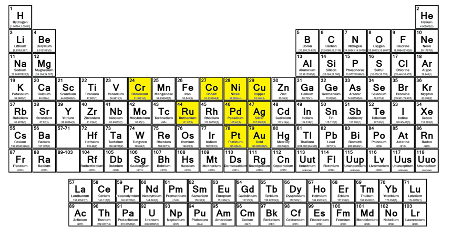
\includegraphics{figures/elpmetals.png}
    \caption{Metals which can be deposited using electro less plating  \cite{Exter2015}}
    \label{fig:elpmetals}
\end{figure}

There are two reported ways of creating palladium alloys through electroless plating; co-plating, and sequential plating. Co-plating has only been reported for Pd-Ag alloys since both palladium and silver have the same reducing agent.\cite{Kikuchi1991, UEMIYA1991303} Co-plating may seem like the optimal manufacturing method since it cuts down on the number of steps required it is generally unsuitable for membrane production since the silver content of the bath must be lowered to at least 7\% in order to prevent dendritical growth, and even then it is difficult to achieve a defect free layer while maintaining plating bath stability. \cite{Exter2015}

Sequential plating involves plating layers on top of each other and forming thge alloy in a subsequent step. For example if a Pd-Ag membrane is desired a palladium layer would first be plated followed by a silver layer. \cite{Exter2015} The membrane would then be annealed under a high temperature in order to achieve a homogeneous alloy. 

\section{Density functional theory for screening of membrane alloy compositions}

Density functional theory (DFT) is a computationa quantum mechanical modelling method which is used to investigate the electronic structure of many body systems, in particular that of atoms, molecules and condensed phases. The method operates by providing an approximate solution to the Schrödinger equation of many body systems. This allows for prediction and calculation of material behaviour based purely on quantum mechanics, eliminating the need for fundamental material properties or experimental data. DFT techniques evaluate the electronic structure of a system by assuming a potential is acting on each of the systems electrons. 

DFT-based methods prove to be useful in applications where a large number of elements and compositions must be investigated to optimize the desired material. For our application DFT calculations can be theoretically used to investigate, and quickly screen the suitability of any atomic configuration in the periodic table in combination with any of the ISO 14687-2 impurities. Much of the work in DFT screening of palladium membranes has been performed by the group of David S. Scholl who have suggested 5 criteria to ensure the application of DFT to the field of palladium membranes are performed in an optimal manner.\cite{SHOLL2007462}, \cite{doi:10.1021/ar500018b} These five criteria are:

\begin{enumerate}
    \item The timescale and/or cost for predictions made using DFT should be shorter than it would take to perform the same tests experimentally
    \item There should be minimal input from experimental data
    \item Predictions must be made on propreties relevant to the end-use application
    \item Quantitative data should be suffieicnt to make confident judgements on whether a material is promising or unpromising
    \item The drawbacks and assumptions associated with DFT should be clearly stated to allow judgement on the predictions impact on real-world situations
\end{enumerate}

This section will provide a a brief overview into DFT. This will include the key concepts required to perform DFT, different assumptions which can be made along with their advantages and disadvantages, and how these relate to our chosen application, screening of metal alloy membranes. Previous work relating to the use of DFT to predict the performance of palladium alloy membranes will be discussed and finally we will tie our planned work back to Scholl's criteria.

\subsection{Key concepts}
\subsubsection{Simulating crystalline structures}
DFT is focused on applying calculations to arrangements of atoms that are periodic in space. DFT calculations achieve this by defining the shape of the 'cell' which will be repeated periodically in space. \cite{doi:10.1002/9780470447710.ch2}

In crystalline solids, which this thesis will focus on, the atoms are arranged in a periodic fashion which repeats after a certain length. In order to explain the crystal structure in this manner a concept called 'reciprocal space' or 'k space' is used. Using this concept planes can be defined as having coordinates within a crystal lattice. These coordinates are referred to as k-points and allow for the structure of a system to be calculated and therefore solved to it's lowest energy state. \cite{doi:10.1002/9780470447710.ch2}

The most effective and widespread solution was developed by Monkhorst and Pack which is implemented into most DFT packages, allowing users to simply define the number of k-points in each direction of reciprocal space. Frequently the same number of k-points are used in each direction. \cite{doi:10.1002/9780470447710.ch4}

The number of k-points used is important to the accuracy of the performed calculation, however higher k-points involve a larger number of calculations across the supercell in reciprocal space and therefore will result in higher calculation times for the whole system. \cite{doi:10.1002/9780470447710.ch4} Convergence is often used to find the optimal number of k-points. This concept is visualised in figure \ref{converge}

\begin{figure}[H]
    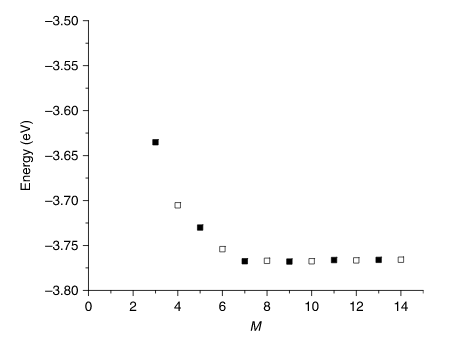
\includegraphics[width=\linewidth]{figures/convergereal.png}
    \caption{Total energies (per atom) for bulk Cu calculated as a function of M for calculations using MxMxM kpoints \cite{doi:10.1002/9780470447710.ch4}}
    \label{converge}
  \end{figure}

At lower numbers of k-points the total energy of the system is dependent on the number of k-points used. This value eventually converges and at M$>$8 k-points becomes completely independent of the nukmber of k-points used. This should be kept in mind when optimising the output values for any simulated system. K-points can be thought of as sampling points within a defined supercell. \cite{doi:10.1002/9780470447710.ch2}

Defining the supercell which will be repeated in periodic space is a simple process and involves defining the volume for the supercell, along with the number, and position of the atoms residing within. 

Metals are a special case in DFT and require the use of special algorithms to ensure that the energy state of a metallic system can be calculated without a high number of k-values. The two best methods for doing this are the tetrahedron method, or smearing. The tetrahedron method involves defining a tertahedron using a discrete set of k-points. This tertahedron fills the reciprocal space and can be integrated to form at all points in the k space and evaluated. \cite{doi:10.1002/9780470447710.ch2}

Smearing involves forcing the function to be continuously integrated to replace any step functions with a smoother function. Ideally the result of the calculation should be a result which can be extrapolated to the limit where smearing is eliminated. \cite{doi:10.1002/9780470447710.ch2}

When simulating a membrane often a slab geometry is used in order to avoid 'edge effects' where simulation results are skewed because of unique surface boundaries resulting from being at the edge of a supercell. The geometry of such a model is achieved through the generation of a box containing a multilayer atomic slab representing the membrane material with a vaccum layer in the remaining volume. From literature palladium membranes are normally in the fcc material phase \cite{Alique_2018} (with the exception being Pd\textsubscript{40}Cu\textsubscript{60} which is in the bcc phase). It is common to represent this using 3-5 atomic layers of palladium. To create alloys random atoms can be substituted for other elements to achieve the desired alloy composition. 

In order to determine the adsorption energy of impurities on a palladium membrane using DFT both the slab being used to represent the membrane surface, and the individual gas molecule must first be simulated in order to determine their individual ground energy states. Then the gas molecule must be adsorbed onto the surface of the membrane. In a crystalline structure there are often multiple sites which are avaliable for gas adsorption. In an fcc structure such as Pd there are 4 main sites which can be considered, shown in figure \ref{fccsites} \cite{Zeng2009}. Once the site is chosen the simulation is iterated, slightly changing the distances between molecules until the mininum ground state is found and therefore the ground energy level of the system composed of the palladium membrane, and the adsorbed impurity. The adsorption energy, $E_{i_{ads}}$, for the adsorption of a gaseous impurity on the surface is calculated equation \ref{adseqn}. Where $E_{slab + i}$ is the total energy of the relaxed gas-surface system where i is the simulated gas, $E_slab$ and $E_i$ are the total energy of relaxed bare surface and gas molecule respectively. Since a system will always tend towards it's lowest energy state, if the total energy of the $E_{i,ads}$ is lower than the sum of it's component energies, it indicates an affinity for the target impurity to adsorb onto the surface of the membrane.

\begin{figure}[H]
    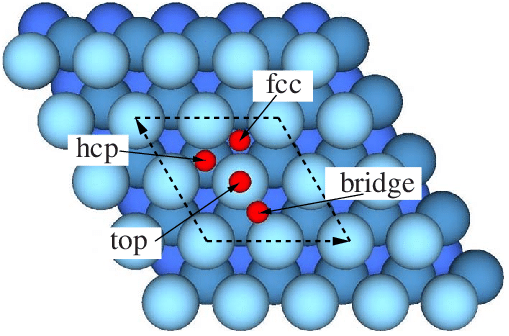
\includegraphics[width=\linewidth]{figures/fccsites.png}
    \caption{Top view of the high-symmetry adsorption sites fcc, hcp, bridge, and top \cite{Zeng2009}}
    \label{fccsites}
  \end{figure}

\begin{equation} \label{adseqn}
    E_{i,ads} = E_{slab} + E_i - E_{slab + i}
\end{equation}

\subsubsection{Approximations}
The ultimate goal of DFT is to calculate the ground-state energy of the defined system. This was shown by Kohn, Holberg and Sham who discovered that this could be found by finding a self-consistent solution to a set of single particle equations, as an exchange correlation. A major complication to this however is that a gaurenteed exchange correlation function simply does not exist, therefore they must be approximated. Two common methods for approximating exchange correlations are local density approximation (LDA) and generalized gradient approximation (GGA)

\paragraph{LDA} is where the energy of the system is assumed to depend on the electron density. LDA is able to predict the energy of a structure to within 1-2\% of the experimental value. Unfortunately the method fails when looking to predict magnetic properties of materials and the band gaps calculated generally tend to overshoot the bond strengths. \cite{dftbook1}

\paragraph{GGA} is an improvement over LDA and takes into account the gradient of electron density as well ad the average electron density. This adds an extra layer of computational complexity. it allows for strucural properties to be predicted to within 1\% of the experimental values and the total energy to be calculated to 1 kJ/mol. \cite{dftbook1} This is also claimed in literature \cite{Olsen2003}.

This thesis will mainly focus on the solid state chemistry in the bulk of the material. For this reason GGA functionals have been chosen as they been shown in numerous publications to perform well. 

\subsubsection{Pseudopotentials}
A pseudopotential is a method used to replace the electron density of a chosen set of core electrons in an atom with a smoothed density chosen to match the physical and mathematical properties of the ionic core of the atom. \cite{dftbook1} The use of a pseudopotential is extremely important in reducing computational burden by reducing the number of planes calculated within the atom. This is commonly referred to as the 'frozen core' assumption whereby only the behaviour of the outer most electrons are calculated, and the inner electrons, whose behaviour has previously been calculated, is considered fixed. \cite{dftbook1}

The main differentiating feature between different tyupes of pseudopotentials is the mininum energy cutoff for each atom in an equation. The mioninum energy cutoff value refers to the number of plane wave functions which will be used to represent the system, a higher cutoff value means that more plane wave functions are used to represent the bahviour of electrons. The most commonly used pseudopotentials are ultrasoft pseudopotentials which feature a relatively low energy cutoff, making them extremely computationally efficient. A disadvantage of using an ultrasoft pseudopotential is that they require the use of empirical values in defining the properties of the core. However a review of various types of pseudopotentials found that there is virtually no difference in results regardless of what pseudopotential is used and this only becomes a factor whern more complex phenomena such as magnetic properties have to be considered. \cite{dftbook1}

Calculations that do not use a pseudopotential are called 'all electron' calculations. However their use is limited due to increased computational burden.  \cite{dftbook1}

\subsection{Use cases, and limitations}

Most work revolving around the use of DFT to predict the adsorption strength of impurities on palladium and palladium alloy surfaces has focused on catalysis of chemical reactions. As a result there are a limited number of papers focusing on quantifying the interaction between these key hydrogen impurities and membranes. Papers which use DFT to predict the behaviour of hydrogen impurities on the surface of palladium membranes are shown in table \ref{DFTREV} . The most relevant study performed by Ozdogan et al \cite{ozdogan2010}  studied the effect of H\textsubscript{2} and H\textsubscript{2}S adsorption energies when small additions of Cu and Nb were added to the membrane composition. The results indicated that while the addition of Cu and Nb hindered hydrogen adsorption, they had a large effect on the adsorption ennergy of H\textsubscript{2}S, concluding that Nb has a higher affinity for H\textsubscript{2}S compared to Pd and a lower addinity for Cu. The results were correlated with experimental results and found to be within 1\% error which is consistent with results found from using GGA. 

Another useful study from Herron et al \cite{HERRON20121670} studied the adsorption of a variety of atomic species (H, O, N, S, and C), molecular species (N\textsubscript{2}, HCN, CO, NO, and NH\textsubscript{3}), and molecular fragments (CN, NH\textsubscript{2}, NH, CH\textsubscript{3}, CH\textsubscript{2}, CH, HNO, NOH, and OH) on the face of Pd(111) to quantify it's effectivness at catalysing a variety of industrial reactions. Depsite it's target application not being membranes, the results are still relevant to our desired study since a number of the molecular species and molecular fragments tested can be expected to be found in hydrogen. As well as quantifying the binding enmergies of all these molecules, the potential energies also indicated that the only reaction thermochemically preferable is the decomposition of NO. Which gives further evidence that reactions such as water gas shift occuring during catalysis are of no concern. 

Outside of these the technique has seen use in predicting the stability of palladium and palladium alloy membranes. A number of studies have successfully combined data from density functional theory to calculate the solubility, diffusivity and permeability of PdCu (\cite{Kamakoti569}, \cite{KAMAKOTI2003145}, \cite{Kamiko2005}), PdAg(\cite{Sonwane2006}, \cite{doi:10.1021/jp064507t}, \cite{doi:10.1063/1.3656739}), PdAu(\cite{Sonwane2006}, \cite{doi:10.1021/jp064507t}, \cite{doi:10.1063/1.3656739}), and ternary alloy (\cite{Kamakoti2006}, \cite{SEMIDEYFLECHA2010384},\cite{LING2011189} membranes. In particular the study by Morreale et al showed that DFT can be used predict experimental data, although to a limited degree as experimental results were approximately 7 times greater than simulated results. \cite{Morreale2007}. The greatest challenge when attempting to describe the permeation of hydrogen through metallic membranes is frequent disordering of atoms during the simulation runtime, throwing off results. Other methods such as cluster expansion have been employed in order to overcome this. 

The fundamental limitation of using DFT to accurately predict the behaviour of materials is that ultimately such calculation usually calculate, at a maxinum, interactions between 10-30 of atoms at a time. This is in no way similar to a physical system where the number of atoms is likely to be in the millions.\cite{dftbook1}It must be understood that DFT calculations draw results from extremely small numbers of atoms, and while relevant to phsycal systems, are likely to result in some errors because of this. \cite{dftbook1}

DFT is also known to be inaccurate in describing systems where weak van der walls attractions exist between molecules and atoms. \cite{dftbook1} This is due to the fact that such attractions are a result of temporary fluctuations in electron density. In order to describe the effect of these interactions on a quantum mechanic level it is necessary to use high level wave function based methods which DFT is unable to accuratly predict. This explains why research only focuses on predicting one molecule on a surface at a time, while multiple molecules could theoretically be placed in a simulation, due to the lack of intermolecular forces being taken into account such results are likely to be innacurate. \cite{dftbook1}

Despite these drawbacks DFT analysis is a useful tool for screening of potential palladium alloy membrane. The technique is capable of speeding up material development by eliminating options that are unlikelym to work, cutting down on trial and error. Due to inacuracies in the technique however it is unlikely that it will ever become a standalone technique in membrane research and it's findings should always be backed up by experimental data.


\eject \pdfpagewidth=11.7in \pdfpageheight=11.7in

    \begin{longtable}{@{\extracolsep{\fill}}C{1in} cc C{1.1in} cc C{1.2in} C{1.2in} c@{}}    
        \caption{Review of DFT studies for adsorption of ISO 14687-2 impurites and hydrogen on palladium membrane surfaces}\label{DFTREV}
        \\
    \toprule
    Simulated material & Structure & Approximation & Exchange function & K-points & Adsorbed species     & Adsorption site        & Binding energy (eV) & ref\\ \midrule  \endfirsthead 
    
    \midrule  \endhead

    \bottomrule \endfoot

    \bottomrule \endlastfoot
    Pd      &    4x4x4 unit cell    & GGA     & PW91                            & 5x5x1      & H\textsubscript{2} &  hcp  & - 0.5485 & \cite{ozdogan2010}         \\

    Pd      &    4x4x4 unit cell    & GGA     & PW91                            & 5x5x1      & H\textsubscript{2} &  fcc  & - 0.5927 & \cite{ozdogan2010}         \\


    Pd      &    4x4x4 unit cell    & GGA     & PW91                            & 5x5x1      & H\textsubscript{2}S &  bridge-fcc-top (H-H-S)  & - 0.7 & \cite{ozdogan2010}         \\

    Pd      &    4x4x4 unit cell    & GGA     & PW91                            & 5x5x1      & H\textsubscript{2}S &  bridge-bridge-top (H-H-S)  & - 0.707 & \cite{ozdogan2010}         \\

    Pd      &    4x4x4 unit cell    & GGA     & PW91                            & 5x5x1      & H\textsubscript{2}S &  bridge-hcp-top (H-H-S)  & - 0.707 & \cite{ozdogan2010}         \\

    Pd      &    4x4x4 unit cell    & GGA     & PW91                            & 5x5x1      & H\textsubscript{2}S &  fcc-hcp-top (H-H-S)  & - 0.692 & \cite{ozdogan2010}         \\

    PdNb\textsubscript{1.6}      &    4x4x4 unit cell    & GGA     & PW91                            & 5x5x1      & H\textsubscript{2} &  hcp  & -0.4259 & \cite{ozdogan2010}         \\

    PdNb\textsubscript{1.6}      &    4x4x4 unit cell    & GGA     & PW91                            & 5x5x1      & H\textsubscript{2} &  fcc  & -0.4740 & \cite{ozdogan2010}         \\

     PdNb\textsubscript{1.6}      &    4x4x4 unit cell    & GGA     & PW91                            & 5x5x1      & H\textsubscript{2}S &  bridge-fcc-top (H-H-S)  & - 0.803 & \cite{ozdogan2010}         \\

     PdNb\textsubscript{1.6}      &    4x4x4 unit cell    & GGA     & PW91                            & 5x5x1      & H\textsubscript{2}S &  bridge-bridge-top (H-H-S)  & - 0.704 & \cite{ozdogan2010}         \\

     PdNb\textsubscript{1.6}      &    4x4x4 unit cell    & GGA     & PW91                            & 5x5x1      & H\textsubscript{2}S &  bridge-hcp-top (H-H-S)  & - 0.735 & \cite{ozdogan2010}         \\

     PdNb\textsubscript{1.6}      &    4x4x4 unit cell    & GGA     & PW91                            & 5x5x1      & H\textsubscript{2}S &  fcc-hcp-top (H-H-S)  & - 0.682 & \cite{ozdogan2010}         \\

     PdNb\textsubscript{1.6}      &    4x4x4 unit cell    & GGA     & PW91                            & 5x5x1      & H\textsubscript{2}S &  hcp-bridge-top (H-H-S)  & - 0.602 & \cite{ozdogan2010}         \\

    PdCu\textsubscript{1.6}      &    4x4x4 unit cell    & GGA     & PW91                            & 5x5x1      & H\textsubscript{2} &  hcp  & -0.4946 & \cite{ozdogan2010}         \\

    PdCu\textsubscript{1.6}      &    4x4x4 unit cell    & GGA     & PW91                            & 5x5x1      & H\textsubscript{2} &  fcc  & -0.5357 & \cite{ozdogan2010}         \\

    PdNb\textsubscript{1.6}      &    4x4x4 unit cell    & GGA     & PW91                            & 5x5x1      & H\textsubscript{2}S &  bridge-fcc-top (H-H-S)  & - 0.429 & \cite{ozdogan2010}         \\

    PdNb\textsubscript{1.6}      &    4x4x4 unit cell    & GGA     & PW91                            & 5x5x1      & H\textsubscript{2}S &  bridge-hcp-top (H-H-S)  & - 0.431 & \cite{ozdogan2010}         \\

    Pd      &    2x2x4 unit cell    & GGA     & PW91                            & 3x3x1      & N\textsubscript{2} &  top  & - 0.23 & \cite{HERRON20121670}         \\
    Pd      &    2x2x4 unit cell    & GGA     & PW91                            & 3x3x1      & N\textsubscript{2} &  fcc  & - 0.02 & \cite{HERRON20121670}         \\
    Pd      &    2x2x4 unit cell    & GGA     & PW91                            & 3x3x1      & N\textsubscript{2} &  bridge  & - 0.07 & \cite{HERRON20121670}         \\

    Pd      &    2x2x4 unit cell    & GGA     & PW91                            & 3x3x1      & NH\textsubscript{3} &  top  & - 0.62 & \cite{HERRON20121670}         \\

    Pd      &    2x2x4 unit cell    & GGA     & PW91                            & 3x3x1      & NH\textsubscript{2} &  top  & -1.63 & \cite{HERRON20121670}         \\

    Pd      &    2x2x4 unit cell    & GGA     & PW91                            & 3x3x1      & NH\textsubscript{2} &  bridge  & -2.15 & \cite{HERRON20121670}         \\

    Pd      &    2x2x4 unit cell    & GGA     & PW91                            & 3x3x1      & NH &  fcc  & -3.45 & \cite{HERRON20121670}         \\

    Pd      &    2x2x4 unit cell    & GGA     & PW91                            & 3x3x1      & NH &  hcp  & -3.30 & \cite{HERRON20121670}         \\

    Pd      &    2x2x4 unit cell    & GGA     & PW91                            & 3x3x1      & CO &  top  & -1.29 & \cite{HERRON20121670}         \\

    Pd      &    2x2x4 unit cell    & GGA     & PW91                            & 3x3x1      & CO &  fcc  & -1.95 & \cite{HERRON20121670}         \\

    Pd      &    2x2x4 unit cell    & GGA     & PW91                            & 3x3x1      & CO &  hcp  & -1.96 & \cite{HERRON20121670}         \\

    Pd      &    2x2x4 unit cell    & GGA     & PW91                            & 3x3x1      & CO &  bridge  & -1.77 & \cite{HERRON20121670}         \\    
    
    Pd      &    2x2x4 unit cell    & GGA     & PW91                            & 3x3x1      & CH\textsubscript{3} &  top  & -1.67 & \cite{HERRON20121670}         \\

    Pd      &    2x2x4 unit cell    & GGA     & PW91                            & 3x3x1      & CH\textsubscript{2} &  bridge  & -3.56 & \cite{HERRON20121670}         \\

    Pd      &    2x2x4 unit cell    & GGA     & PW91                            & 3x3x1      & CH &  fcc  & -5.91 & \cite{HERRON20121670}         \\

    Pd      &    2x2x4 unit cell    & GGA     & PW91                            & 3x3x1      & CH &  hcp  & -5.89 & \cite{HERRON20121670}         \\

    Pd      &    2x2x4 unit cell    & GGA     & PW91                            & 3x3x1      & CH &  hcp  & -5.89 & \cite{HERRON20121670}         \\

    Pd      &    2x2x3 unit cell    & GGA     & PW91                            & 3x3x1      & H\textsubscript{2} &  top  & -0.07 & \cite{Olsen2003}         \\

    Pd      &    2x2x3 unit cell    & GGA     & PW91                            & 3x3x1      & H\textsubscript{2} &  bridge  & -0.37 & \cite{Olsen2003}         \\

    Pd      &    2x2x3 unit cell    & GGA     & PW91                            & 3x3x1      & H\textsubscript{2} &  fcc  & -0.49 & \cite{Olsen2003}         \\

    Pd      &    2x2x3 unit cell    & GGA     & PW91                            & 3x3x1      & H\textsubscript{2} &  hcp  & -0.45 & \cite{Olsen2003}         \\

    PdAg\textsubscript{25}      &    2x2x3 unit cell    & GGA     & PW91                            & 3x3x1      & H\textsubscript{2} &  top  & 0.84 & \cite{Olsen2003}         \\
    
    PdAg\textsubscript{25}      &    2x2x3 unit cell    & GGA     & PW91                            & 3x3x1      & H\textsubscript{2} &  bridge  & -0.27 & \cite{Olsen2003}         \\

    PdAg\textsubscript{25}      &    2x2x3 unit cell    & GGA     & PW91                            & 3x3x1      & H\textsubscript{2} &  fcc  & -0.22 & \cite{Olsen2003}         \\

    PdAg\textsubscript{25}      &    2x2x3 unit cell    & GGA     & PW91                            & 3x3x1      & H\textsubscript{2} &  hcp  & -0.22 & \cite{Olsen2003}         \\




    \end{longtable}
    \eject \pdfpagewidth=8.3in \pdfpageheight=11.7in


\section{Conclusion}
This chapter provided a review of the hydrogen process, from how hydrogen is produced and it's relationship to the impurites which can end up in the supply chain. The effect of these impurities on the operation of a fuel cell electric vehicle was discussed and the liklihood of these impurities reaching a consumers fuel cell. 

Different methods for enriching hydrogen was discussed with one of the most promising methods identified being hydrogen impurity enrichment using a dense metal membrane. From here a number of membrane materials designed to separate hydrogen from multicomponent mixtures. An extensive summary has been provided on the separation performance and stability of these materials with an emphasis on the complications related to transitioning the use of these materials from laboratory and  R\&D efforts, to industrially relevant processes. The key observation is that while there is a large research focus on new membrane materials, there is a lack of research looking into the engineering of these membranes into functional systems and products. Out of the hundreds of materials being researched for gas separation, commercially only four-eight different polymers are being used, with some niche applications using palladium membranes. Research focus should shift towards focusing on repeatability, scale up, and creating engineered systems where new membrane materials can be used in order to make progress in bringing these new materials to market. Out of the membrane materials reviewed palladium based alloys were the most appropriate to be used for hydrogen impurity enrichment and focus in this thesis will be to find a suitable composition for measuring ISO 14687-2 impurities while minimising interaction with reactants. 

DFT based theories were discuessed and identified as a method to save time money and cost when attemtping to optimise the palladium alloy composition. There is a gap in research on using this technique for palladium alloys specifically targeting ISO 14687-2 impurities. While limited literature exists since many papers adress the use of palladium surfaces as catalysts the research is useful for creating a starting base. Palladium alloy membranes can be screened for materials which exhibit the lowest reactivity with ISO 14687-2 impuruties, and once identified, they can be manufactured and tested. It is important to note however that there are a number of innacuracies involved in the technique and should only be used as a rough guide. 

\bibliographystyle{unsrtnat}



\bibliography{library.bib}

\chapter{Experimental methods}
\section{Introduction}

\section{Preparation of gas standards} \label{gasprep}
Gas standards of hydrogen were prepared gravimetrically in 10 litre cylinders (BOC, UK) in accordance with \cite{InternationalStandardISO6142-1:2015} from pure hydrogen (Air Products, UK), nitrogen (Air Products), carbon monoxide (Scott Speciality Gases, UK), methane (CK Gases, UK) and krypton (BOC, UK). Any impurities that were detected in these pure gases were quantified and these values were then incorporated into the final determination of the gas mixture compositions and uncertainties. 

For the purpose of this thesis the gas standards that were used to perform the permeation tests will be referred to as gas mixtures, and the gas standards that were used to calibrate the analytical instruments will be referred to as calibration gas standards. Before use, the gas mixtures were verified against traceable primary reference materials using Gas Chromatography with either a pulsed helium discharge ionisation detector (PDHID) for samples not containing sulphur [Reference for DN34], and sulphur chemiluminescence detector (SCD) for sulphur containing samples [Reference for B543]. The compisitions of the non-sulphur, and sulphur contining gas standards created for the purposes of this thesis are shown in tables \ref{nonsulf} and \ref{sulf}.

\begin{table}[]
    \centering
    \caption{Gas mixture composition of the non-sulphur sample (Cylinder NG353R) used during impurity tests}
    \label{nonsulf}
    \begin{tabular}{@{}cc@{}}
    \toprule
    Impurity & \begin{tabular}[c]{@{}c@{}}Concentration \\ ($\mu$mol/mol)\end{tabular} \\ \midrule
    O\textsubscript{2}       & 10.06 ± 0.241 \%                                                              \\
    N\textsubscript{2}       & 10.04 ± 0.377 \%                                                               \\
    CH\textsubscript{4}      & 10.01 ±0.096 \%                                                               \\
    CO\textsubscript{2}      & 10 ± 0.082 \%                                                                 \\
    CO       & 9.98 ±  0.085 \%                                                                \\
    H\textsubscript{2}       & Balance                                                             \\ \bottomrule
    \end{tabular}
    \end{table}

    \begin{table}[]
        \centering
        \caption{Gas mixture composition of the sulphur sample (Cylinder 2380) used during impurity tests}
        \label{sulf}
        \begin{tabular}{@{}cc@{}}
        \toprule
        Impurity & \begin{tabular}[c]{@{}c@{}}Concentration \\ (umol/mol)\end{tabular} \\ \midrule
        Kr       & 1.1 ± 1.056 \%                                                                \\
        H\textsubscript{2}S      & 0.41 ± 0.346\%                                                                \\
        OCS      & 0.42       ± 0.322 \%                                                               \\
        CS\textsubscript{2}      & 0.362 ±  0.316 \%                                                              \\
        t-BuSH   & 0.391 ± 0.315\%                                                               \\
        THT      & 0.409  ± 0.319\%                                                             \\
        H\textsubscript{2}       & Balance                                                             \\ \bottomrule
        \end{tabular}
        \end{table}


\section{Membrane preparation}

\subsection{Materials used}
\subsection{Support fabrication}\label{supportmake}
The YSZ 3\% hollow fibre substrates with a sponge like microstructure were fabricated by an induced phase-inversion process, followed by high temperature sintering. A uniform ceramic suspension, with 60 wt.\% solid loading YSZ 3\% powder (1μm, VWR), was prepared by ball milling. After degassing, the ceramic suspension was transferred into 200 mL stainless steel syringes and extruded through a tube-in-orifice spinneret (outer diameter 3 mm, inner diameter 1.2 mm) into a coagulation bath with no air gap. An extrusion rate of 7 and 5 mL min\textsuperscript{-1} was adopted for ceramic suspension and bore fluid (15 wt.\% 1,4- dioxane in n-hexane) respectively. The formed precursor fibres were kept in deionized water for a minimum of 12 h, in order to remove the excess solvent. After being gently washed with deionized water, the precursor fibres were dried at room temperature and sintered at 1400\textdegree C in a tubular furnace (Elite, Model TSH 17/75/450).

\subsection{Membrane deposition}
\subsubsection{Electoless Plating}\label{elpproc}
Palladium silver, copper, gold, and ternary alloy compositions (expect for PdCuZr) were deposited onto the surface of the porous YSZ substrate through electroless plating. The process was performed in the two step activation-plating process discussed in section \ref{lit-ELPREV}. Palladium was used due to its high electro positivity compared to other metals commonly plated through electroless deposition. 

Prior to deposition, the outer surface of the fibre was cleaned by sequential washings with a 1:1 mixture of ethanol and water for 10 min in an ultrasonic bath, and were then dried overnight at 120\textdegree C. The substrates were then coated at one end with a gas tight glaze and sintered at 900\textdegree C for 1 hour. The outer surfaces of the fibres were cleaned by sequential washings with a 1:1 mixture of ethanol and water for 10 min in an ultrasonic bath, and were then dried overnight at 120 \textdegree C.

\begin{table}[]
  \centering
  \caption{Compositions used for activation of YSZ substrate prior to palladium deposition}
  \label{pretreat}
  \begin{tabular}{@{}ccccc@{}}
  \toprule
  \multicolumn{1}{l}{\multirow{2}{*}{Compound}} & \multicolumn{4}{c}{Concentration (g/L)}             \\ \cmidrule(l){2-5} 
  \multicolumn{1}{l}{}                          & Sensitisation & Washing & Activation & Acid Washing \\ \midrule
  SnCl\textsubscript{2}                                         & 1             & -       & -          & -            \\
  PdCl\textsubscript{2}                                         & -             & -       & 0.1        & -            \\
  HCl                                           & 1             & -       & 1          & 0.01           \\ \bottomrule
  \end{tabular}
  \end{table}

\begin{table}[]
    \centering
    \caption{Compositions used for preparation of palladium based membranes on YSZ substrate through electroless plating and immersion plating}
    \label{ELP}
    \begin{tabular}{@{}ccccc@{}}
    \toprule
    \multirow{2}{*}{Compound} & \multicolumn{4}{c}{Deposited metal} \\
                              & Pd      & Ag     & Cu      & Au     \\ \midrule
    Metal Source (g/L)        &         &        &         &        \\ \midrule
    PdCl\textsubscript{2}                     & 4       & -      & -       & -      \\
    AgNO\textsubscript{3}                     & -       & 3.4    & -       & -      \\
    CuSO\textsubscript{4}                     & -       & -      & 10      & -      \\
    AuCl\textsubscript{3}                     & -       & -      & -       & 0.1    \\ \midrule
    \multicolumn{5}{c}{Stabilising agent}                           \\ \midrule
    NH\textsubscript{3}-H\textsubscript{2}O (mL/L)            & 198     & 200    & -       & -      \\
    NaOH (g/L)                & -       & -      & 8.63    & 1      \\ \midrule
    \multicolumn{5}{c}{Complexing Agent (g/L)}                      \\ \midrule
    Na\textsubscript{2}EDTA-2H\textsubscript{2}O              & 40      & 35     & -       & -      \\
    Persulfate                & -       & -      & 30      & -      \\ \midrule
    \multicolumn{5}{c}{Reducing agent (mL/L)}                       \\ \midrule
    N\textsubscript{2}H\textsubscript{4}                      & 5.6     & 4.2    & -       & -      \\
    Formaldehyde              & -       & -      & 14      & -      \\ \bottomrule
    \end{tabular}
    \end{table}

The substrates were then activated with Pd nuclei via sensitisation in an acidic SnCl\textsubscript{2} solution, followed by activation in an acidic PdCl\textsubscript{2} solution. The sensitisation/activation 
process was carried out by immersing the glazed hollow fibre substrates sequentially in five chemical baths, i.e. acidic SnCl\textsubscript{2} solution for 5 min; deionised water for 5 min, acidic PdCl\textsubscript{2} solution for 5 min; 0.01 M HCl solution for 2 min; and finally deionised water for 3 mins. 
All chemical baths were homogenised using compressed air. The sensitisation/activation process was repeated for 8 cycles. The composition of each bath is shown in Table \ref{pretreat}.

\begin{figure}
    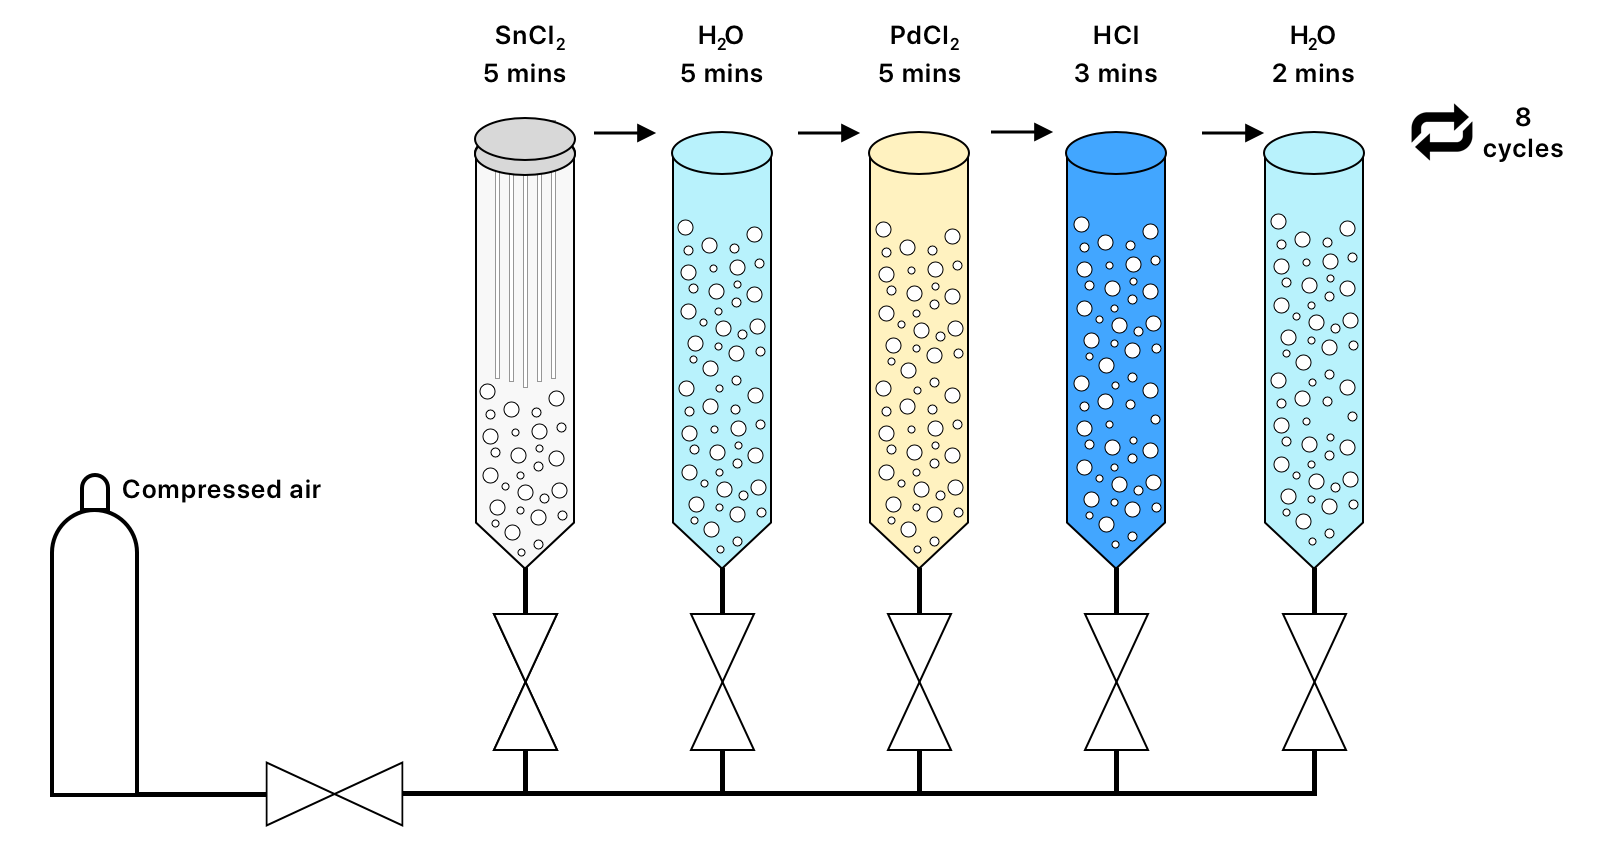
\includegraphics[width=\linewidth]{figures/pretreatment.png}
    \caption{Schematic representation of the sequential baths for sensitisation/activation process.}
    \label{sintering}
  \end{figure}

The substrates were then immersed in a Pd electroless plating (ELP) solution, at 60\textdegree C, in order to deposit metallic Pd layers onto the activated surface. The Pd ELP solution was prepared according to the composition presented in Table \ref{ELP} taken from \cite{GouveiaGil2015} for Pd, \cite{Braun2014} for Ag, \cite{Pomerantz2009}  and left to stabilize for 1 h in an ultrasonic bath prior to use. The volume of Pd ELP solution was fixed at 4 mL per cm\textsubscript{2} of 
substrate surface area. The electroless plating procedure was performed twice, with a total plating time of 60 mins.

After the palladium coating the membranes were then subjected to one, or multiple, other plating steps of silver, gold, or copper. The plating time for silver was 30 minutes for one cycle and the volume of plating solution to substrate was the same as the palladium steps.

It should be noted that the deposition of gold is through immersion plating rather than electroless plating. \cite{adawiyah_azlina_fadil_aisha_hanim_2016} Immersion plating is the process of applying adhering layers of nobler metals to another metal's surface by dipping the material in a heated nobler metal solution ion to produce a replacement reaction. This causes the deposition of a metallic coating on a base metal from solutions that contain coating metal. One metal is typically displaced by metal ions that have lower levels of oxidation potential, relative to the metal ion being displaced. The plating time for gold was 3 hours and the volume of plating solution to substrate was 4mL/cm\textsuperscript{3}. 

The resulting composite membranes consisting of multiple metal layers stacked were then heat treated at 500\textdegree C under an environment containing 25\% H\textsubscript{2} in Ar balance for 24 hours in order to alloy the layers into a homogenous membrane and reduce any oxides that were present on the surface.


\begin{figure}
    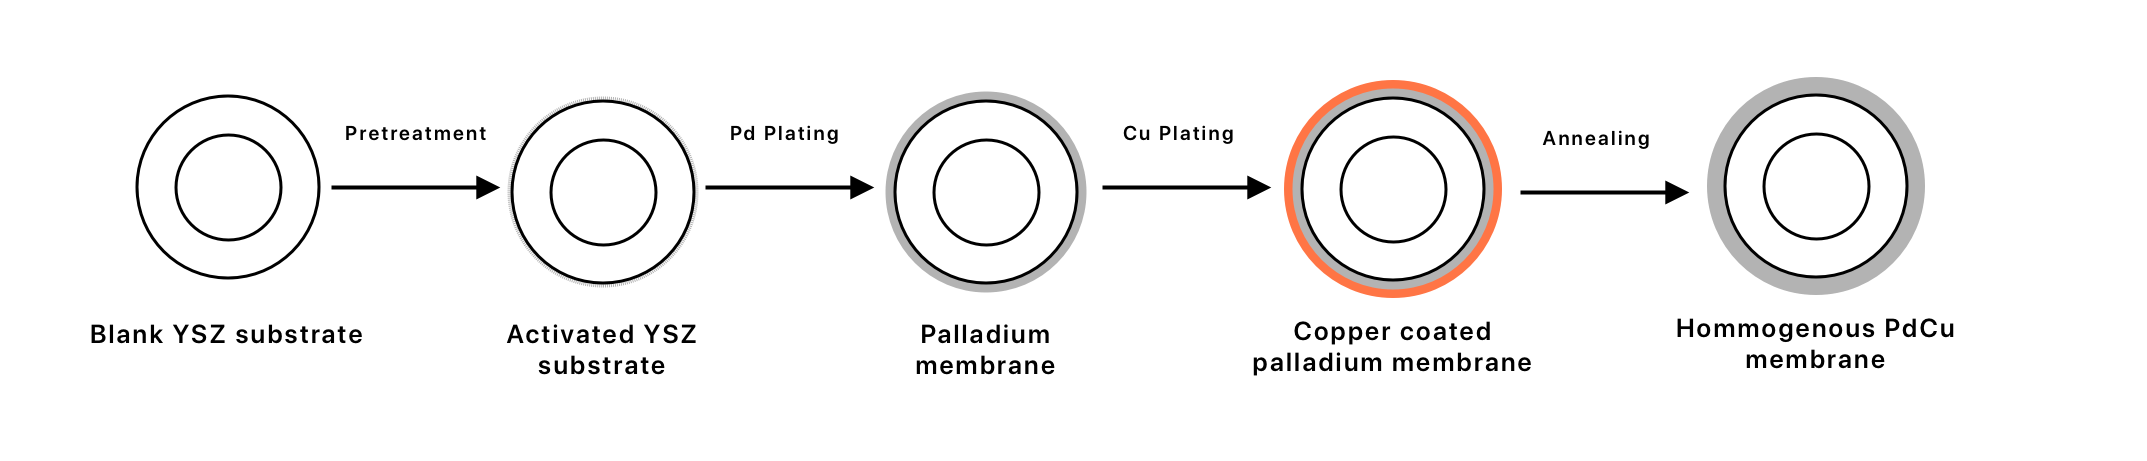
\includegraphics[width=\linewidth]{figures/ELpprocedure.png}
    \caption{Example of ELP procedure when manufacturing a PdCu membrane on YSZ substrate}
    \label{ELP Procedure}
  \end{figure}

\subsubsection{Magnetron Sputtering}\label{msproc}
Membranes were deposited using a closed field unbalanced magnetron sputter ion plating system produced by Teer Coatings Ltd. The thin film membranes were deposited onto the YSZ 3\% hollow fibres by mounting them vertically inside the sputtering system. The system was then evacuated to 1x10\textsuperscript{-6} mBar and subjected to an ion cleaning process with Ar plasma prior to sputtering. Pd, Cu, and Zr targets (99.9\% purity) were used to sputter the chosen alloy composition onto the membranes at the target currents shown in. A bias voltage of 50 V was applied to the magnetron during deposition runs. Samples were deposited using pulsed DC, with a constant target to substrate distance and a sample rotation speed of 16 rpm. An Ar flux of 25 (SCC/m) was used during deposition. PdCu membranes in both BCC and FCC phase were manufactured through magnetron sputtering along with PdCuZr ternary alloys. 

\begin{table}[]
    \centering
    \caption{Conditions used during magnetron sputtering of palladium membranes on YSZ tubular substrate}
    \label{sputtering}
    \begin{tabular}{@{}cccc@{}}
    \toprule
    \multirow{2}{*}{Alloy} & \multicolumn{3}{c}{Target current (A)} \\
                           & Pd          & Cu          & Zr         \\ \midrule
    PdCuZr                 & 1.25        & 0.65        & 0.4        \\
    PdCu (fcc)             & 1.25        & 0.8         & -          \\
    PdCu (bcc)             & 1.2         & 1.0         & -          \\ \bottomrule
    \end{tabular}
    \end{table}

\subsection{Materials testing}\label{MatTest}
The thickness of the plated layers was characterised by first using a Focused Ion Beam (FIB) to mill through a section of the hollow fibre to provide a flat, cross sectional surface for analysis. The thickness of the metal later was then measured using high resolution Scanning Electron Microscopy (SEM) and composition analysed using Energy Dispersive x-ray Spectrometry (EDS) on the same sample. 

The surface composition of the membrane was further characterised using X-ray Photoelectron Spectroscopy to provide a more accurate compositional analysis for the top 10 nm of the membrane, the depth which is most relevant for catalytic dissociation of hydrogen and adsorption of impurities.

Prior to the H\textsubscript{2} permeation tests, the integrity of the hollow fibre membranes was evaluated by testing the gas-tightness of the membrane under N\textsubscript{2} atmosphere, up to 10 bar and room temperature and using a gas-tightness apparatus developed in house. \cite{GouveiaGil2015}

\section{Membrane Characterization}

\subsection{Membrane testing rig}
After the membranes were ensured to be gas tight, hydrogen permeation measurements were performed using the experimental apparatus shown in Figure 1. The palladium alloy composite hollow fibre membranes were sealed on to a stainless steel ¼” NPT fitting. The membrane was then placed in a Sulfinert®-treated sample vessel (Thames Restek, UK) with nominal volume of 300 cm\textsuperscript{3}. The vessel was then heated using heavy insulated heating tape (OMEGA STH051-020). The heating was controlled using the temperature of the membrane using a PID temperature controller (OMRON). The feed was supplied from a cylinder either containing BIP+ hydrogen (Air Products) for pure hydrogen permeability tests or one of two gravimetrically prepared gas mixtures for impurity testing shown in tables \ref{nonsulf} and \ref{sulf}. Prior to introducing gas to the membrane the system was evacuated down to 1 x 10\textsuperscript{-6} mbar. The pressure on the retentate side of the membrane is controlled using a tamper proof pressure reducer. The set-up is shown in figure \ref{testrig}. After tests the system was vented and purged 7 times with N\textsubscript{2} to ensure an explosive atmosphere could not build up within the equipment.

The flux and permeability of the membrane were automatically calculated using software developed in house. Each membrane sample was made using the same batch of substrate and cut to the same length prior to testing. The permeability (P)  of a dense metal membrane is given by Eqn \ref{eq:1} \cite{NathanW.Ockwig2007} and is a function of the hydrogen flux through the membrane (J), the concentration and pressure gradient across the membrane ($P^{0.5}_{ret}-P^{0.5}_{perm}$), and the thickness of the metallic membrane (l). 

\begin{equation} \label{eq:1}
    P = \frac{J l}{P^{0.5}_{ret}-P^{0.5}_{perm}}
\end{equation}

\begin{landscape}
\begin{figure}[h]
  \centering
  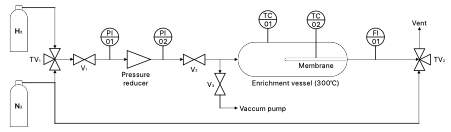
\includegraphics[decodearray={0.2 0.5}, width=0.9\linewidth, height=\textheight,  keepaspectratio]{/Users/marc/Thesis/Experimental/perm_rig.png}
  \caption{Experimental set up used during hydrogen permeation and enrichment experiments, TC: Temperature controller, PI: Pressure indicator, V: Valve, TV: Three-way valve,  FI: Flow indicator.}
  \label{testrig}
\end{figure}

\end{landscape}

\section{Hydrogen impurity enrichment}\label{enrichproc}
A hydrogen impurity enrichment device was designed and tested, more details on this will be discussed in chapter 6. This section will describe the methodology and testing procedure for the hydrogen impurity enrichment device. 

Hydrogen impurity enrichment tests were performed on synthetic samples created using the procedure described in section \ref{gasprep} and using a sample taken from a hydrogen refuelling station. Regardless of source all samples were tested using a PDHID in order to calculate it's oxygen level for safety reasons. Since only hydrogen can leave the HIED in normal testing conditions, if not checked the concentration of oxygen could rise above a safe level and create an explosive mixture. For the purpose of these tests the enrichment factor was capped at a value that would ensure the oxygen level in the mixture would not surpass 1\%. 

The enrichment factor was calculated using both non-ideal gas law (equation \ref{lit-eq:1}), and tracer enrichment (equation \ref{lit-eq:2}) methods. This was to ensure any leaks in the device could be detected using non-ideal gas law method, while having a low uncertainty on the final value from the tracer enrichment method. Gas composition testing was performed using the same GC procedures discuessed in section \ref{gasprep}
\subsection{Krypton spiking}
In order to perform enrichment using the tracer enrichment method a certain quantity of inert gas, not normally present within a hydrogen sample, must be included in the gas. Krypton was used in this study. For synthetic samples this can be added using loop addition along with other impurities using the procedure in section \ref{gasprep}. When taking a sample directly from a hydrogen refuelling station, as would have to be done in real sampling, this approach is not effective as the tracer gas cannot be added to an already pressurised container. The krypton must first be added to the evacuated sampling vessel through loop addition.

Since sampling from a hydrogen refuelling station is dependent on a number of variables, it is difficult to determine the final pressure of the sample. Therefore, a fixed quantity of krypton gas was added to the cylingers. For the purpose of this thesis, since 10L cylinders were used for the purpose of hydrogen sampling, 0.24g of Kr was added through loop addition as this is enough to ensure at a max fill pressure of 100 bar there would be atleast 70 \textmu mol/mol, which is well within the range of the GC-PDHID detector, and avaliable gas standards for validation. 

\subsection{Performing enrichment}
The protocol for performing hydrogen impurity enrichment is similar to hydrogen permeation tests. After evacuation the gas is introduced to a vessel containing the chosen palladium membrane composition at a set enrichment pressure and the vessel heated to 300\textdegree C to begin enrichment. The pressure of the enrichment vessel and sample cylinder were both monitored and their values used to calculate the enrichment factor in real time using equations \ref{lit-eq:1} and \ref{lit-eq:2}. Once the desired enrichment factor was achieved the heater was switched off and the enrichment vessel isolated. The enrichment vessel was then brought to the desired GC detector and it's composition tested against a gas standard as described in section \ref{gasprep}

\section{Density functional theory} \label{DFTparams}
All DFT calculations were performed using the Quantum Espresso (QE) \cite{QE-2009, QE-2017, doi:10.1063/5.0005082} ab initio simulation package using the generalized gradient approximation with the PW91 functional to describe electron-correlation effects. Ion-electron interactions were described using ultra-soft pseudopotentials. A plane-wave expansion with a cut-off energy of 233.73 eV was used in all calculations. Geometry relaxations were performed with a conjugate gradient method until the forces on all unconstrained atoms were less than 0.03 eV/A. A Monkhorst Pack mesh with 5x5x5 k-points was used for all calculations as this was determined to be adequate for achieveing convergence from literature in table \ref{lit-DFTREV} and backed up by initial testing on a Pd system as shown in figure \ref{kpoints}.

\begin{figure}
  \centering
  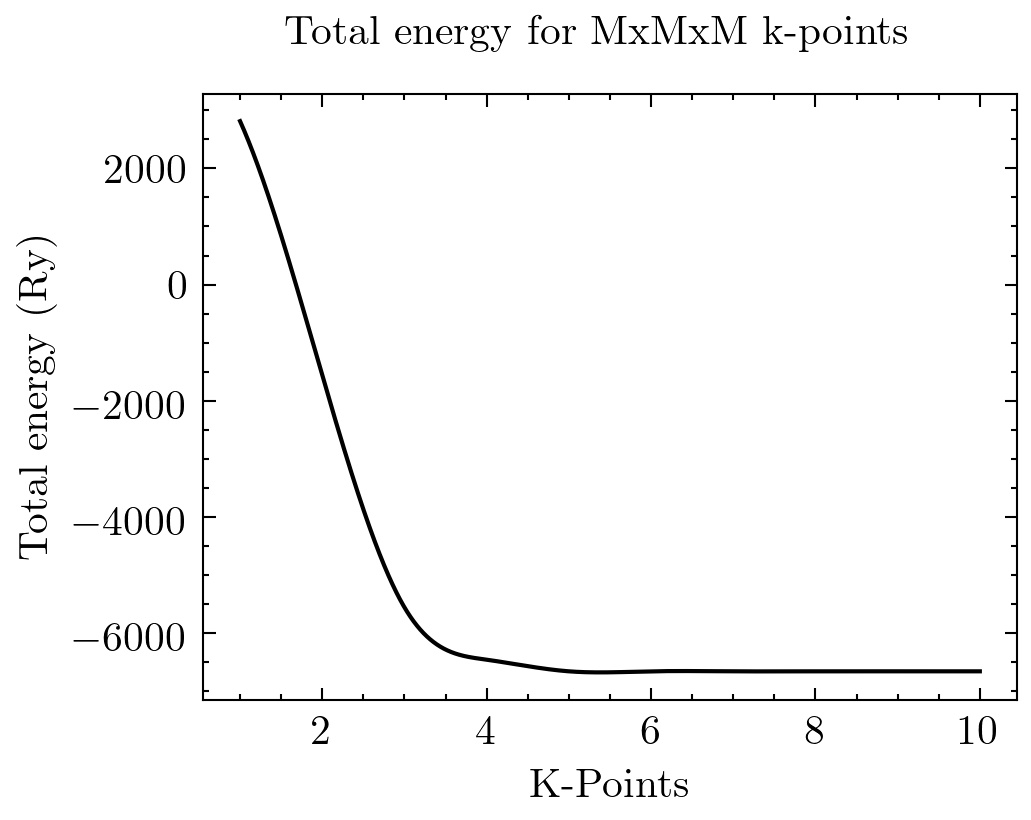
\includegraphics[width=\linewidth, height=0.45\textheight,keepaspectratio]{/Users/marc/Thesis/Experimental/kpoints.jpg}
  \caption{Total energy as a function of $M\times M\times M$ k-points across a Pd(111) fcc slab}
  \label{kpoints}
\end{figure}

Python with scikit learn, pandas, numpy, and matplotlib packages were used for scripting, data collection and analysis. Sample files can be found in Appendix 3. 

\subsection{ISO 14687 Impurities and Hydrogen} \label{gassim}
ISO 14687 impurities were simulated using the above parameters and their structure relaxed until convergence was achieved. The resulting structure was then cross checked using bond lengths from literature to ensure the resulting molecule was an accurate representation. 

\subsection{Palladium and Palladium alloy slab models}\label{slabsim}
The structure of bulk palladium was first created using a lattice parameter of 3.859\si{\angstrom} as reported by D. Wheeler \cite{PhysRev.25.753}. Initially the pure palladium slab model used to represent the periodic supercell was created using this palladium primative unit cell cleaved using the miller indices $(h,k,l) = (111)$ which is adequate in describing the surface of a palladium membrane. A $2\times 2$ slab was created in order to ensure minimal in-plane interactions between neighbouring molecules adsorbed onto the surface in the periodic simulations. The slab was extended to 5 atom thickness which is adequate to describe the surface of Pd(111) and a 20\si{\angstrom} vaccum layer was placed on top. The resulting supercell consisted of 20 atoms. 

When creating palladium alloy systems it was assumed that alloys adopt a substitutional, random fcc structure. Metal atoms were randomly distributed among the fcc lattice in the supercell. All atoms were allowed to relax during the calculation, with the volume of the super cell fixed. 

Quantum ATK Virtual NanoLab Builder \cite{synopsys} was used to generate these structures and export to QE input files. Each metal composition was simulated with three random distributions of substituted metal. For each alloy, geometry optimization was performed to get the lattice constant and total energy of each alloy prior to adsorption of gaseous molecules.

\subsubsection{Adsorption energy}
In order to find the adsorption energy of each ISO 14687 impurity on the membrane surfaces the molecules simulated in section \ref{gassim} were inserted into the vacuum region of the slab models generated in section \ref{slabsim}. (111) fcc surfaces have 4 available sites for adsorption shown in figure \ref{lit-fccsites} A separate system was created for adsorption of each impurity onto each of these sites. Initially the adsorbed molecule was simulated using a ridgid constraint to prevent any changes to the impurities molecular structure, and a low cutoff energy in order to get a quick starting point for the basis of the full simulation. Final goemetry relaxation was then performed from this using the parameters described in section \ref{DFTparams}

The adsorption energy, $E_{i_{ads}}$, for the adsorption of a gaseous impurity on the surface is then calculated using equation \ref{lit-adseqn} where $i$ is the target ISO 14687 impurity or hydrogen molecule.



\renewcommand{\bibname}{References}
\bibliographystyle{unsrtnat}
\bibliography{library.bib}

\chapter{Density functional theory as a screening method for dense metal membranes}

\section{Abstract}

\section{Introduction}
High impurity resistant dense metal membranes are being developed for hydrogen impurity enrichments of HRS samples with hydrogen derived from biomass, hydrocarbon or electrolysis. Metal membranes operate by selectively dissociating hydrogen, which then allows the hydrogen atoms to solubilize and subsequently permeate through the bulk of the separation layer. The problem is that many hydrogen impurities are also capable of adsorbing onto and interacting with the surface of many of the metals which comprise dense metal membranes. The impact of this adsorption can vary depending the molecule, Carbon monoxide for example will simply adsorb onto the surface and result in competitive adsorption between the hydrogen and impurity. Sulphur containing impurities which are commonly found in hydrocarbon sources and therefore are potentially present in any hydrogen produced from these methods. Sulphur containing impurities present more of a problem since they can potentially react with many metals used for hydrogen separation membranes. The impact of these contaminants can be minimized by designing alloy compositions that have a weaker attraction to the membrane, and therefore will have less of an affect at higher temperatures where these membranes operate.

Physically testing each potential membrane composition would be time consuming and costly due to the high price of palladium, the time required to synthesise specific membrane compositions, and performing the tests. Simulations provide a solution to this, allowing potential alloys to be screened for their interaction strength with each individual ISO 14687-2 impurity quickly, avoiding the cost of manufacturing each alliy composition. 

This chapter will calculate the behaviour of 56 palladium alloy composition under 13 ISO 14687-2 impurities. This is done by comparing the total energy of different configurations after relaxation of internal forces in the system. The close packed surfaces of palladium alloys were simulated as 

The pure metals and alloy slabs were modelled as slabs with periodic boundary conditions in the two directions parallel to the surface and separated by at 10A thick vaccum region. 

\section{Results and discussion}
The adsorption energy, $E_{i_{ads}}$, for the adsorption of a gaseous impurity on the surface is calculated using:

\begin{equation}
    E_{i,ads} = E_{slab} + E_i - E_{slab + i}
\end{equation}

Where $E_{slab + i}$ is the total energy of the relaxed gas-surface system where i is the simulated gas, $E_slab$ and $E_i$ are the total energy of relaxed bare surface and gas molecule respectively. Since a system will always tend towards it's lowest energy state, if the total energy of the $E_{i,ads}$ is lower than the sum of it's component energies, it indicates an affinity for the target impurity to adsorb onto the surface of the membrane.

\begin{table}[]
    \centering
    \caption{Simulated total energy values of ISO 14687-2 impurities}
    \label{gases}
    \begin{tabular}{@{}cc@{}}
    \toprule
    Gas          & \begin{tabular}[c]{@{}c@{}}Total Energy\\ $(kJ \times 10^{-21})$\end{tabular} \\ \midrule
    H            & -2.01                                                               \\
    N\textsubscript{2}           & -123.91                                                             \\
    O\textsubscript{2}           & -180.86                                                             \\
    CO           & -130.93                                                             \\
    CO\textsubscript{2}          & -221.95                                                             \\
    NH\textsubscript{3}          & -1933.22                                                            \\
    Ar           & -208.10                                                             \\
    CH\textsubscript{4}          & -50.73                                                              \\
    Formaldehyde & -136.13                                                             \\
    Formic Acid  & -227.08                                                             \\
    H\textsubscript{2}S          & -150.36                                                             \\
    He           & -12.62                                                              \\
    H\textsubscript{2}O          & -95.99                                                              \\ \bottomrule
    \end{tabular}
\end{table}

\subsection{Stability of palladium alloy compositions}

\begin{table}[]
    \centering
    \caption{Simulated total energy values of alloy slabs}
    \label{slabs}
    \resizebox{\textwidth}{!}{\begin{tabular}{@{}ccccc@{}}
    \toprule    
    Alloy/Metal Composition   & Space group   & Calculated lattice parameter (A)   & \begin{tabular}[c]{@{}c@{}}Total Energy\\ (ry)\end{tabular} & Total Energy kJ \\ \midrule
    Pd           & -      &-6653.38       & -                                     & -1.45x10-17     \\
    PdAg23       & -      &-6774.37       & -                                     & -1.48 x10-17    \\
    PdAu10       & -      &-7545.53       & -                                     & -1.64x10-17     \\
    PdAu20       & -      &-8437.613      & -                                     & -1.84x10-17     \\
    Pd60Cu40     & -      &-5703.15       & -                                     & -1.24x10-17     \\
    Pd80Cu20     & -      &-6178.29       & -                                     & -1.35x10-17     \\
    Pd70Au20Zr10 & -      &-8389.61       & -                                     & -1.83x10-17     \\
    Pd70Cu20Zr10 & -      &-6130.29       & -                                     & -1.34x10-17     \\
    Pd70Ag10Zr20 & -      &-6605.75       & -                                     & -1.44x10-17     \\
    PdZr10       & -      &-6605.45       & -                                     & -1.44x10-17     \\
    PdZr20       & -      &-6557.46       & -                                     & -1.43x10-17     \\
    Pd70Au20Ag10 & -      &-8485.99       & -                                     & -1.84x10-17     \\
    Pd70Au20Cu10 & -      &-8200.05       & -                                     & -1.79x10-17     \\
    Pd70Cu20Ag10 & -      &-6226.71       & -                                     & -1.36x10-17     \\ \bottomrule
    \end{tabular}}
    \end{table}

\subsection{Hydrogen and Impurity adsorption on palladium alloy membranes}
\subsubsection{Hydrogen}
\subsubsection{Helium, Nitrogen and Argon}
\subsubsection{Carbon Monoxide}
\subsubsection{Carbon Dioxide}
\subsubsection{Ammonia}
\subsubsection{Oxygen}
\subsubsection{Water}
\subsubsection{Methane}
\subsubsection{Formaldehyde}
\subsubsection{Formic Acid}
\subsubsection{Hydrogen sulphide}

\section{Conclusion}
\bibliographystyle{plainnat}
\bibliography{library.bib}



\chapter{Impurity resistance of dense metal membranes under hydrogen impurities}\label{testingchapref}
\section*{Abstract}
In this chapter a number of dense palladium alloy membranes were synthesised on a YSZ substrate using a combination of electroless plating and magnetron sputtering in order to determine which membrane compositions resisted impurities. 

The permeability of the synthesised membranes, in addition to a commercial membrane were tested under a variety of ISO 14687-2 impurities in order to determine which alloy composition was most suitable for use as a membrane material for hydrogen impurity enrichment, where low reactivity with impurities present in hydrogen samples are required. Of the tested membranes the best performing compositions were PdAuAg, PdAuCu and PdCuZr which only showed a 27\%, 25\% and 26\% drop in permeability under atmospheres containing 10 ppm of non-sulphurous, and 2 ppm of sulphurous impurities typically expected to be found in hydrogen derived from steam methane reforming.  This indicates that these alloys are most suitable for metrology purposes due to their low reactivity. 

\section{Introduction}
In order to improve the accuracy and the cost of hydrogen impurity enrichment a suitable membrane composition must be found. In addition to this all previous studies used a commercial palladium-based membrane and in all cases it was noted that certain impurities reacted with the membrane. This interaction had the result of changing the composition of the enriched gas muxture and therefore reducing the final accuracy of the measurement. \cite{Murugan2014, Ahmed2010} The self-supported commercial membranes used in both studies are also generally between 20-100 $\mu$m in order to provide sufficient mechanical strength for a membrane. However, for palladium membranes to be economical this thickness must be reduced to about 1-5 $\mu$m giving the added benefit of greater flux and therefore lower enrichment times. 

Palladium alloy membranes are generally created by forming an alloy with silver, copper or gold. By doing this the hydrogen embrittlement effect can be effectively mitigated. Using alloys has the added benefits of decreasing the overall amount of palladium required in the film, driving up their cost effectiveness, and in some cases increasing the flux of the membrane to higher levels achievable than a pure palladium membrane. In the previous chapter a number of membrane compositions were identified to be able to resist certain classes of ISO 14687-2 impurities. The best membranes being identified as PdAu\textsubscript{20} and PdAu\textsubscript{20}Cu\textsubscript{10} for carbonaceous impurities. For sulphur containing impurities PdCu\textsubscript{20}Zr\textsubscript{10}, PdAu\textsubscript{20}Zr\textsubscript{10}, and PdAu\textsubscript{20}Cu\textsubscript{10} were the most resistent to binding with H\textsubscript{2}S.In this chapter these membranes will be manufactured and tested under environments containing these gases in order to verify these results, and quantify the level of reactivity. In addition to these alloys, PdCu\textsubscript{20}Ag\textsubscript{10} and PdAu\textsubscript{20}Ag\textsubscript{10} will be synthesised due to their strong performance in the previous chapter. PdAg\textsubscript{23}, PdCu\textsubscript{20} and PdCu\textsubscript{40} will also be synthesised as these are popular membrane compositions in literature and act as a good benchmark in addition to the commercial membrane. Unfortunately the PdAuZr composition could not be manufactured due to the high cost associated with sputtering gold.

Palladium alloy membranes will be deposited onto porous YSZ supports using both electroless plating  and closed field unbalanced magnetron sputter ion plating as described in sections \ref{exp-elpproc} and \ref{exp-msproc}. This will have the combined effect of reducing the amount of palladium used, driving down their cost, and  increasing the flux, and therefore reducing the time taken to enrich a hydrogen sample. The degree of interaction of impurities with the surface of the membrane will be quantified using a three-step experimental procedure. The pure hydrogen flux of each membrane composition will be measured and the membranes hydrogen permeability calculated as a base line. The following two permeation tests will measure the change in permeability resulting from introducing part-per-million level impurities into the gas sample. The change in permeability which results from this will act as a measure for the membranes tendency to interact with different impurity types. Additionally, at all three testing stages, X-ray photoelectron spectroscopy (XPS) will be performed on the surface of the membranes to investigate how the composition on the surface of the membrane changes when exposed to each impurity environment. This will allow the alloy segregation behaviour to be observed, and more importantly, quantify the amount of sulphur which has reacted with the surface of the membrane. 

\section{Results and Discussion}
\subsection{Membrane characterisation}

Figure \ref{fig:1} (a)-(g) shows the cross-sectional SEM images of the manufactured membranes.  The thickness of the fabricated membranes are shown in \ref{results:1} and ranged from 573 nm to 1.579 $\mu$m. In general thinner layers were achieved using electroless plating although theoretically sub-micron layers are possible through magnetron sputtering, examples of this being SINTEF’s patented sputtering process.\cite{Peters2011} The integrity of the manufactured membranes was measured using the procedure laid out in section \ref{exp-MatTest}. All membranes showed no leakage when pressurised to 10 bar indicating that all membranes were uniform, pinhole free and therefore suitable for hydrogen separation. \cite{GouveiaGil2015}

\begin{figure}
    \centering
    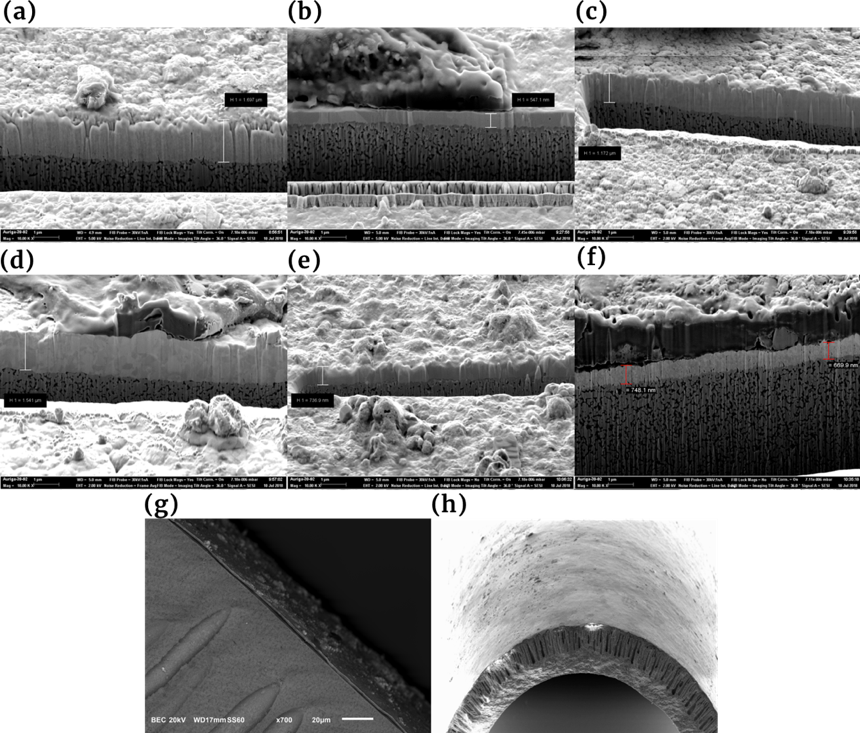
\includegraphics[width=\linewidth, height=0.9\textheight,keepaspectratio]{figures/Semxsect.png}
    \caption{SEM images of fabricated membranes (a) PdCu (fcc) (Sputtering) (b) PdAg (ELP) (c)PdAu (ELP) (d) PdCuZr (Sputtering) (e) PdAgAu (ELP) (f) PdCuAg (ELP) (g) PdCu (bcc) (Sputtering) (h) typical cross section}
    \label{fig:1}
\end{figure}

The surface composition of each membrane was measured by XPS and is shown in Table \ref{results:1}. A wide range of compositions were fabricated. From phase data on the PdCu system \cite{Roa2003, Nayebossadri2013} both varieties of PdCu membranes (bcc phase and fcc phase) were successfully fabricated. 

\begin{table}[]
    \centering
    \caption{Membrane compositions analysed by EDS and their thickness measured using FIB-SEM}
    \label{results:1}
    \resizebox{\textwidth}{!}{\begin{tabular}{@{}cccccccc@{}}
    \toprule
    \multicolumn{1}{c}{\multirow{2}{*}{Membrane ID}} & \multirow{2}{*}{Manufacturing technique} & \multicolumn{5}{c}{Composition (wt\%) (+- 1\% Relative)} & \multirow{2}{*}{Thickness (um)} \\
    \multicolumn{1}{c}{}                             &                                          & Pd        & Cu        & Ag        & Au        & Zr       &                                 \\ \midrule
    PdCu (Fcc)                                        & Magnetron Sputtering                     & 76.24     & 23.76     & -         & -         & -        & 1.679                           \\
    PdCu (Bcc)                                        & Magnetron Sputtering                     & 43.24     & 56.64     & -         & -         & -        & 1.664                           \\
    PdCuZr                                            & Magnetron Sputtering                     & 72.10     & 14.46     & -         & -         & 13.54    & 1.541                           \\
    PdAg                                              & Electroless Plating                      & 65.55     & -         & 34.45     & -         & -        & 0.573                           \\
    PdAu                                              & Electroless Plating                      & 74.7      & -         & -         & 25.3      & -        & 1.172                           \\
    PdCuAg                                            & Electroless Plating                      & 72.1      & -         & 8.27      & 19.58     & -        & 0.867                           \\
    PdCuAu                                            & Electroless Plating                      & 63.90     & 13.6      & -         & 22.1      & -        & 1.545                           \\
    PdAuAg                                            & Electroless Plating                      & 60        & -         & 11.2      & 28.3      & -        & 0.736                           \\ \bottomrule
    \end{tabular}}
\end{table}

% Silver is the most popular dopant for palladium membranes and forms a stable alloy with palladium at concentrations greater than 20 wt\%, with the optimal composition occurring at 23 wt\%. On top of mitigating the effects of hydrogen embrittlement, a $~$60\% increase in permeability is observed when compared to pure Pd membranes. Despite having enhanced permeation properties, PdAg is still susceptible to poisoning, in particular from sulphurous compounds which can form both Pd\textsubscript{4}S and Ag\textsubscript{5}Pd\textsubscript{10}S\textsubscript{5}. A composition of Pd\textsubscript{64.9}Ag\textsubscript{35.1} wt\% was achieved, which, while higher than the desired composition of Pd\textsubscript{77}Ag\textsubscript{23} wt\%, was determined adequate for the purposes of this study.

% Copper is another widely studied binary alloy which is known to suppress hydrogen embrittlement. Alloying with copper also has the advantage that it reduces the cost of the membrane by a larger amount than most other metals and through improving the membranes sulphur resistance. The maximum permeability of a palladium copper membrane occurs at the composition Pd\textsubscript{60}Cu\textsubscript{40} wt\% and this is due to the formation of a bcc lattice rather than the fcc lattice commonly seen in pure palladium and most binary alloys. \cite{She2014} Temperature cycling has previously been performed on this alloy composition and it has been found that the bcc crystalline configuration has a higher permeability than the fcc phase. \cite{Dolan2010} This behaviour is due to the increased number of hcp adsorption sites which hydrogen has a slight preference for, and the bcc structure allowing faster diffusion through the bulk of the membrane. \cite{Wilcox2010} Conversely the fcc structure has a higher impurity resistance than the bcc structure, particularly for H\textsubscript{2}S. \cite{She2014, D.T.Hughes1978} Pd\textsubscript{44}Cu\textsubscript{66} and Pd\textsubscript{65.5}Cu\textsubscript{34.5} wt \%  membranes were manufactured using magnetron sputtering which were in the range for bcc and fcc phases respectively.

% PdAu alloys see a slight increase in permeability, up to 30\% more than pure Pd \cite{Atsonios2015}, with gold additions up to 20\%, after which the permeability rapidly decreases. While alloying with gold does not improve the permeability much compared to silver or copper, gold alloys show greatly improved sulphur resistance. \cite{Chen2010} The synthesised membrane was found to have the composition  Pd\textsubscript{74.7}Au\textsubscript{25.3} which, while containing a high amount of gold resulting in lower permeation, will have a higher impurity resistance. 

\subsection{Hydrogen permeation}
Table \ref{results:2} shows the hydrogen permeation through the 9 tested membranes at steady state after 12 hours of operation. As expected, hydrogen permeation flux increases with the elevated temperatures. Moreover, the mass transfer resistance of the substrate will not represent major limitations since its gas transport resistance is negligible compared to that of the dense palladium alloy layer \cite{GouveiaGil2015}. Deposited layers were all on the scale of 0.5-2 $\mu$m which from previous research indicates the main rate limiting step in hydrogen permeation being the thickness of the membrane layer. \cite{NathanW.Ockwig2007a} The palladium copper alloy which was in the bcc phase showed the highest hydrogen permeability of all the synthesised membranes which was expected as discussed in section \ref{lit-pdreview}. The membrane which showed the lowest hydrogen permeability was the PdCuZr membrane, this is likely due to the combined effects of the alloy having the lowest concentration of palladium compared to the other synthesised membrane, increasing the transport resistance of the membrane, and this composition having a lower preference to hydrogen binding as all other palladium alloys as predicted in the simulations performed in section \ref{dft-Hsection} and shown in figure \ref{dft-h2ads}. The PdAu and PdAuAg membranes both showed low permeabilities. Gold as an alloying material traditionally does not show much increase in permeability \cite{Chen2010}  but is instead used to suppress the effects of impurities on the membrane, \cite{Chen2010} which is the main goal of this study. Despite the fact that the commercial membrane is also based on PdAgAu, the membrane manufactured through electroless plating has a lower permeability due to the high gold concentration. It is likely that the concentration of silver in the commercial membrane is closer to 23\%, which is the optimal value for hydrogen permeation, and it’s gold concentration is much lower than the electroless plated membrane. Both PdCuAg and PdCuAu had reasonably high hydrogen permeabilities. While none of these membranes showed a hydrogen permeability as high as the commercial alloy, it should be noted that the commercial membrane had a much larger thickness resulting in a much higher cost and lower flux values than the composite membranes. 

\begin{table}[]
    \centering
    \caption{Pure hydrogen permeability of studied alloy membranes under pure hydrogen at 300\textdegree C and 1 bar pressure differential}
    \label{results:2}
    \begin{tabular}{@{}cc@{}}
        \toprule
        \multicolumn{1}{c}{Membrane ID} & \begin{tabular}[c]{@{}c@{}}Permeability\\ ($mol\:m^{-1} s^{-1} pa^{1/2} \times 10^{-8}$)\end{tabular} \\ \midrule
        PdCu (Fcc)                       & 1.30                                                                                               \\
        PdCu (Bcc)                       & 1.68                                                                                               \\
        PdCuZr                           & 0.14                                                                                               \\
        PdAg                             & 0.94                                                                                               \\
        PdAu                             & 0.33                                                                                               \\
        PdCuAg                           & 1.22                                                                                               \\
        PdCuAu                           & 1.43                                                                                               \\
        PdAuAg                           & 0.19                                                                                               \\
        Commercial (REB)                 & 5.71                                                                                               \\ \bottomrule
        \end{tabular}
\end{table}


\subsection{Impurity reactivity}

\begin{table}[]
\centering
\caption{Permeability results for all membranes under both impurity conditions}
\label{results:3}
\begin{tabular}{@{}cccccl@{}}
\toprule
\multirow{2}{*}{Membrane ID} & \multicolumn{3}{c}{\begin{tabular}[c]{@{}c@{}}Permeability\\ ($mol\:m^{-1} s^{-1} pa^{1/2} \times 10^{-8}$)\end{tabular}} & \multicolumn{2}{c}{\% Drop} \\
                             & Pure H\textsubscript{2}  & Non-Sulphur & Sulphur & Non-sulphur    & Sulphur    \\ \midrule
PdCu (Fcc)                   & 1.30     & 0.22        & 0.185   & 80\%           & 86\%       \\
PdCu (Bcc)                   & 1.68     & 0.721       & 2.47    & 55\%           & 85\%       \\
PdCuZr                       & 0.14     & 0.12        & 0.101   & 12\%           & 26\%       \\
PdAg                         & 0.94     & 0.117       & 0.007   & 88\%           & 92\%       \\
PdAu                         & 0.33     & 0.165       & 0.215   & 51\%           & 35\%       \\
PdCuAg                       & 1.22     & 0.48        & 0.299   & 61\%           & 75\%       \\
PdCuAu                       & 1.43     & 0.789       & 1.07    & 45\%           & 25\%       \\
PdAuAg                       & 0.19     & 0.163       & 0.142   & 16\%           & 27\%       \\ \bottomrule
\end{tabular}
\end{table}

Table \ref{results:3} shows the results of hydrogen permeation under the presence of the two different impurity conditions discussed in Table \ref{results:3} compared to the pure hydrogen permeability values shown in Table \ref{results:2}. The permeability data was taken once the flux had reached steady state after 12 hours of operation. For all membranes there was a reduction in permeability when the membranes were exposed to impurities. The magnitude of this reduction compared to the pure hydrogen permeability is used as an indication of the degree of interaction between the membrane and the impurities.  Table \ref{results:4} shows the composition of each membrane in between each test in order to measure permanent surface reactions and segregation behaviour of the alloys under the chosen impurities. 

\subsubsection{Binary alloys}
In non-sulphur tests the PdAg binary alloy was the worst performing, with the permeability dropping by 88\% of its original value. This was expected as the addition of silver to a palladium system, while effective at increasing the permeability, does not contribute much to impurity resistance. \cite{Peters2016b} This was further supported by the results of the sulphur tests where the permeability dropped by 92\% and composition analysis in Table \ref{results:4} showing that sulphur was present in 42\% of the surface. The PdAg alloy also showed a large degree of segregation behaviour under non-sulphur impurities which likely contributed to the large reduction in flux, with silver concentration increasing to 75\% at the top 10 nm of the sample, resulting in a large drop in permeability. 

Interestingly the PdCu membrane with a composition in the bcc phase showed higher resistance to non-sulphurous impurities than the fcc phase, with the former only experiencing a 55\% drop in permeability compared to an 80\% drop in permeability in the latter. This again seems to be a result of the segregation behaviour of the alloy, with the PdCu alloy in the fcc phase experiencing a large amount of segregation, with the palladium concentration increasing to around 90\% on the retentate side. Conversely the PdCu composition in the BCC phase membrane only changed slightly. The XPS analysis showed that while the reactivity of sulphur on the surface of both copper based binary membranes was of a similar magnitude, the BCC phase had a slightly lower resistance, with 29\% of the surface containing sulphur after exposure to sulphurous impurities as opposed to the 25\% shown by the fcc phase alloy.

The PdAu alloy showed the best impurity resistance out of the binary alloys tested under both impurity conditions, with only a 51\% and 35\% drop in permeability under non-sulphur and sulphur conditions respectively and only a 12\% concentration of sulphur was observed on the surface after XPS analysis. The alloy showed slight segregation of gold away from the permeate surface under non-sulphur impurity conditions likely due to the fact the difference in interaction strength between gold and palladium with the components of the gas mixture varies widely, with many gases preferentially adsorbing on palladium \cite{Gade2011}.

\begin{landscape}
\begin{table}[]
    \centering
    \caption{XPS composition analysis of the palladium alloy membrane surfaces after impurity tests}
    \label{results:4}
    \begin{tabular}{@{}ccccccccccccccccc@{}}
    \toprule
    \multirow{2}{*}{Membrane ID} & \multicolumn{5}{c}{Pure Hydrogen Exposure} & \multicolumn{5}{c}{Non-Sulphur Exposure} & \multicolumn{6}{c}{Sulphur Exposure} \\
                                 & Pd     & Ag     & Au     & Cu     & Zr     & Pd      & Ag     & Au    & Cu     & Zr   & Pd    & Ag  & Au  & Cu   & Zr & S    \\ \midrule
    PdCu (Fcc)                   & 65.5   & -      & -      & 35.5   & -      & 92.5    & -      & -     & 7.5    & -    & 67.5  & -   & -   & 7.5  & -  & 25   \\
    PdCu (Bcc)                   & 44     & -      & -      & 66     & -      & 54.85   & -      & -     & 45.15  & -    & 40    & -   & -   & 31   & -  & 29   \\
    PdCuZr                       & 63.6   & -      & -      & 22.6   & 13.8   & 64.4    & -      & -     & 27.5   & 8.5  & 54.2  & -   & -   & 27   & 8  & 10.8 \\
    PdAg                         & 65.5   & 34.5   & -      & -      & -      & 25      & 75     & -     & -      & -    & 29    & 29  & -   & -    & -  & 42   \\
    PdAu                         & 75     & -      & 25     & -      & -      & 82.9    & -      & 17.1  & -      & -    & 71    & -   & 16  & -    & -  & 13   \\
    PdCuAg                       & 64.6   & 9.1    & -      & 26.3   & -      & 8.6     & 8.9    & -     & 82.5   & -    & 6     & 5   & -   & 64   & -  & 25   \\
    PdCuAu                       & 63.9   & -      & 22.5   & 13.6   & -      & 84.9    & -      & 1.46  & 13.6   & -    & 65.3  & -   & 1   & 18.5 & -  & 15.2 \\
    PdAuAg                       & 60     & 11.7   & 28.3   & -      & -      & 47.2    & 49.8   & 3     & -      & -    & 52    & 35  & 1   & -    & -  & 12   \\ \bottomrule
    \end{tabular}
    \end{table}
\end{landscape}
\subsubsection{Ternary alloys}
Five ternary alloy compositions were tested including the commercial alloy. The commercial alloy had the highest permeability of all ternary alloys with a value of 5.71 mol m\textsuperscript{-1} s\textsuperscript{-1} pa\textsuperscript{-0.5}x10\textsuperscript{-8} under pure hydrogen and 4.28 mol m\textsuperscript{-1} s\textsuperscript{-1} pa\textsuperscript{-0.}5x 10\textsuperscript{-8}  under non-sulphur conditions, a drop in permeability of 25\%. However, the commercial membrane nearly lost all of its permeability under sulphurous conditions. The PdAuAg membrane manufactured through electroless plating performed better under both impurity conditions than the commercial alloy despite being based on the same composition, only seeing a 16\% and 27\% drop in hydrogen permeability under non-sulphur and sulphur conditions respectively compared to a 25\% and 96\% drop shown by the commercial alloy. The high levels of gold likely contributed to the low levels of sulphur on the surface of the electroless plated PdAuAg membrane. These results indicate that the composition of the commercial membrane, while ideal for separation, does not contain enough gold to withstand the levels of sulphur impurities expected for analytical purposes. 

The worst performing ternary alloy was the PdCuAg alloy which showed large permeability drops under all conditions, 61\% under non-sulphur and 75\% under sulphurous conditions. In addition to these, large degrees of segregation were observed under non-sulphur impurities, with the palladium concentration at the surface dropping to 8.5 wt\%, showing that the alloy is not completely stable under the varying conditions expected during analytical purposes.  

Both gold containing ternary alloys, PdAuAg and PdCuAu, performed well under sulphur conditions, with the PdCuAu alloy only reducing in permeability by 25\% and the PdAgAu membrane by 27\%. The PdCuAu membrane however had a stronger interaction with non-sulphur impurities, indicated by the permeability drop of 45\% when exposed to the non-sulphur containing gas sample. This drop is likely due to the segregation of palladium to the surface with the XPS data indicating an increase of palladium to the surface to 84.9 wt\% from 63.9\%. The best performing ternary membrane was the PdCuZr membrane which showed the smallest drop in permeability of only 12\% non-sulphur conditions, and a permeability percentage drop of 26\% under sulphur conditions which on a similar magnitude to that of the gold containing alloys.
\begin{landscape}
    
\begin{figure}
    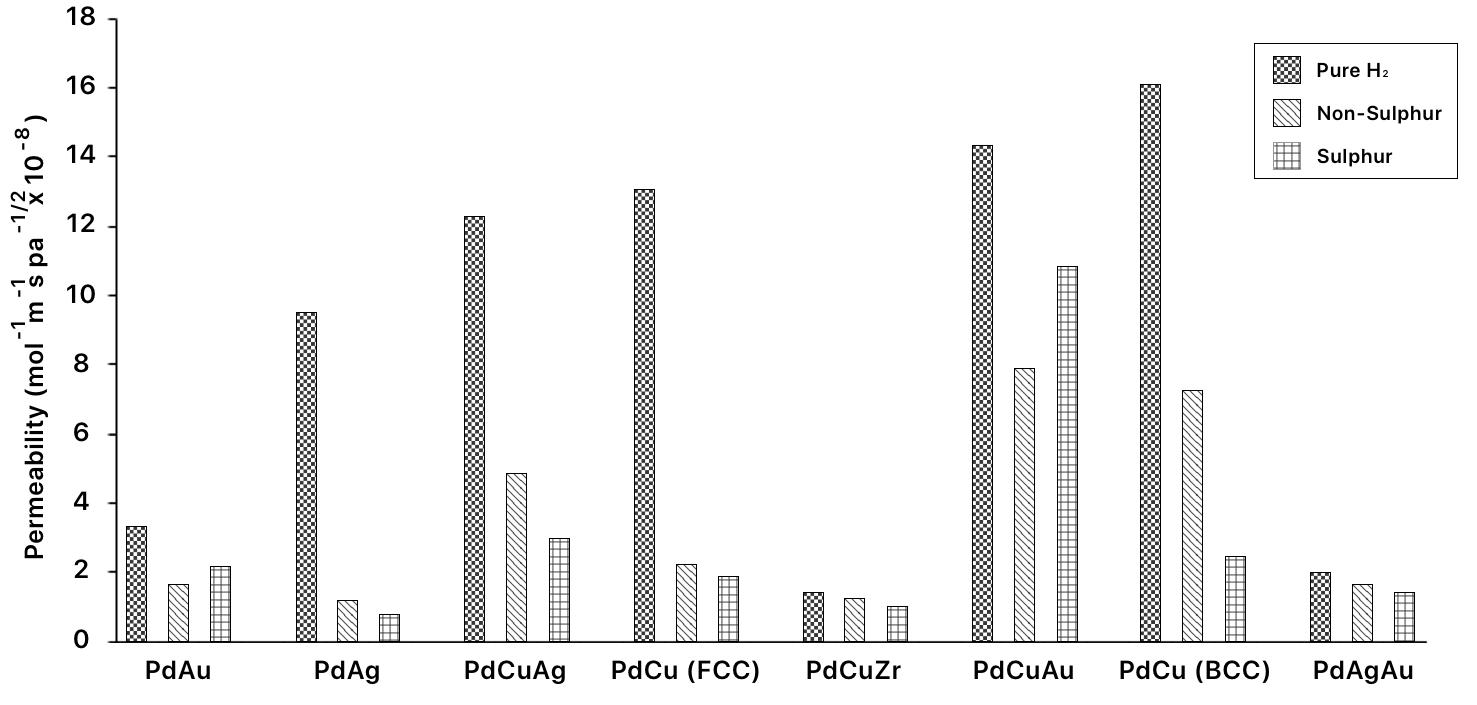
\includegraphics[width=\linewidth]{figures/permeabilitychart.png}
    \caption{Permeability data for pure hydrogen, non-sulphur, and sulphur permeation tests}
    \label{permgraph}
  \end{figure}
\end{landscape}

\subsubsection{Segregation behaviour}
All membranes tested showed some degree of segregation with the two thinnest membrane samples, PdAg (0.573 micron), PdAuAg (0.736  micron) and PdCuAg (0.873 micron) all showing the highest degrees of segregation. While this may still be a property of the alloy compositions it may also indicate that sub-micron palladium alloys layers are unstable and there may be a minimum thickness for alloys, below which the membrane layer is unstable and frequently varies during operation.

\subsection{Relationship to DFT results}
The previous chapter attempted to use DFT generated binding energies to predict the perfomance of alloy composistions in environments containing ISO 14687-2 impurities. While a useful analysis it appears in some cases that these results were not completely correct and could be improved in further studies. 

For carbonaceous environments the model predicted that PdAu20 and PdAuCu would be the best performing alloys. PdAuCu experienced a 45\% drop in permeability under carbonaceous environments while PdAu\textsubscript{20} experienced a 51\% drop. Which while showing reasonable resistance, were inferiour to both the PdCuZr and PdAuAg alloys which only experienced a 12\% and 16\% drop respectivley. For the PdAuAg alloy the model did indeed predict that it would resist adsorption to these impurities, and agrees with the conclusion of this alaysis that the addition of gold and silver improves the alloys resistence to carbonaceous impurities. However appears to be completely incorrect, with all models predicting that the alloy would be more susceptible to poisoning. 

The model fared better when predicting the influence of sulphurous impurities on the surface of the membrane. The model successfully predicted that both PdCuAu and PdCuZr alloys would be the most resistent to sulphurous environments. The model appears to be accurate in predicting how the other alloys would react in the environment, indicating the PdAg, PdCuAg, and both FCC and BCC PdCu alloys would perform poorly and see severe levels of sulphur poisoning. It should be noted that many of the results in this section were close and other alloys which performed reasonably well against sulphur poisoning (PdAu\textsubscript{20} and PdAuAg) could be as a result of the error between simulations. 

The DFT simulations were a useful tool in predicting the sulphur resistance of the alloys, however when used to predict the behaviour of weaker adsorbing compounds, such as the carbonaceous impurities, it appears to break down. This is likely due to the fact that DFT is not as effective at simulating the behaviour of weaker bonds as discussed in section \ref{lit-DFTLIMS}. Alternative methods should be explored if these interactions are to be predicted.

\section{Conclusion}
In order to identify a suitable palladium alloy composition for hydrogen impurity enrichment, eight different membrane compositions were manufactured and tested under three different hydrogen conditions against a commercial palladium membrane. Two different measures were used to compare the membrane compositions suitability for hydrogen impurity enrichment, the permeability deviation from the pure hydrogen permeability was used as an initial indicator of interaction between the alloy and impurities, and the surface composition was measured to detect any impurities which had permanently reacted with the membrane. 

The best performing membrane, and therefore the most suitable for hydrogen impurity enrichment was the PdCuZr alloy, which only showed a 12\% and 26\% drop in permeability under non-sulphur, and sulphur conditions, and low levels of sulphur on the surface. The permeability of this alloy was low, however, surface areas could easily be scaled up to increase the speed of hydrogen enrichment. 

In the following chapter this membrane will be used in the design of the hydrogen impurity enrichment device and it's performance measured when tested with a real hydrogen fuel sample.

\bibliographystyle{unsrtnat}
\bibliography{library.bib}

\chapter{A hydrogen impurity measurement device for measuring ISO 14687 impurities}

\section{Abstract}
In this chapter a device capable of performing hydrogen impurity enrichment is designed and tested under a number of conditions using a commercial membrane compared against the best performing fabricated membranes in chapter 5. The aim of this chapter is to improve upon the designs in literature to provide a more efficient, and safe device which could be sold as a commercial product. A sample was taken from a commercial hydrogen refuelling station, spiked with krypton, and enriched using the device in order to validate the krypton tracer enrichment method using real world conditions, and to quantify the impurity concentrations present in commercial hydrogen fuel. 

\section{Introduction}


\section{Results and discussion}

\section{Conclusion}
% \bibliographystyle{plainnat}
% \bibliography{library.bib}

\chapter{Enriching impurities in hydrogen refuelling station samples}

\section*{Abstract}
In this chapter the HIED  was tested under a number of conditions using a commercial membrane compared against the best performing fabricated membranes in chapter 5. 

Enrichment was performed using a number of synthetic hydrogen samples created using the procedure outlined in section \ref{exp-gasprep}, and a hydrogen sample taken from a hydrogen refuelling station. The device was capable of enriching samples to 85 times. Theoretically higher enrichment factors were possible but these tests were limited for safety reasons. The commercial membrane took 7 days to perform this measurement and provided the final value of within 2\% of the gravimetrically calculated value using the tracer enrichment method which was deemed sufficient for a commercial device. The device was also tested using a sulphur containing sample which resulted in failure of all membranes. The PdCuZr membrane while identified as being a strong candidate for enriching sulphurous impurities, failed in all tests due to poor thermal stability of the support. The commercial membrane on the other hand reacted with the gases in the mixture and became completely inactive. 

For the first time a sample was taken dierctly from a hydrogen refuelling station and enriched. The sample was enriched 46 times and was found to have 22 ppm of nitrogen, and a small amount of argon which was not visible during other tests, further showing that the method can be used to quantify impurities past the limit of detection normally achievable.   

\section{Introduction}
Now that appropriate membrane compositions have been found, a number of improvements must be made to the hydrogen impurity enrichment device in order to make it suitable as a commercial process and product for measuerment of ISO 14687-2 impurities. All previous devices used were extremely manual and required close operator attention to ensure the experiment performed correctly. All enrichment factor calculations discussed in section \ref{exp-enrichproc} must also be calculated by hand, after the experiment has been performed, limiting the ability for the operator to plan the experiment in advance. In addition to this the krypton enrichment method which was identified as the best method for calculating the enrichment factor in section \ref{lit-enrichlit} but no procedure is in place to instruct operators on how to add this krypton to their sampling vessel. 

This chapter will provide a method for taking krypton spiked samples from a hydrogen refuelling station, improve the hydrogen impurity enrichment device through automation to improve the usability of the device, while providing real time results for the user, and quantify how the enrichment device performs when tested using a real sample froma  hydrogenr refuelling station. 

\section{Enrichment of hydrogen samples}
Enrichment of the hydrogen samples was performed using the set up shown in figure \ref{hiedpid}. An initial test was performed using a commercial membrane supplied by REB using an inert mixture created using the procedure in section \ref{exp-gasprep} in order to calculate the uncertainty associated with the device. Both the commercial and PdCuZr membrane identified as the best performing membrane in chapter 5 were tested using a synthetic gas mixture containing sulphur containing compounds, and krypton. Finally both the commercial membrane and PdCuZr membrane were tested using a sample taken from the hydrogen refuelling station using the procedure outlined in section \ref{exp-sampletake}.

In each case the system was purged 7 times with the hydrogen sample to ensure there was no air present in the system. Enrichment was performed at a temperature of 300\textdegree C and a final enrichment pressure of 5 bar. Enrichment factors were calculated using both the tracer enrichment method (equation \ref{lit-eq:2}) calculated at the end of the test, and non-ideal gas law method (\ref{lit-eq:2}) calculated using the data processing script described in section \ref{HRS-dataproc}.

The gas mixtures used in the inert and sulphur tests are shown in table \ref{inert} and \ref{exp-sulf}. Prior to testing the HRS sample was tested to verify the concentration of krypton, and ensure there was no oxygen present in the system to pose as a hazard. Enrichment factors were capped at 100 to ensure any residual oxygen would not reach a high enough concentration to create an explosive environment.

\begin{table}[]
    \centering
    \caption{Gas mixture composition of the inert sample used during enrichment tests}
    \label{inert}
    \begin{tabular}{@{}cc@{}}
    \toprule
    Impurity & \begin{tabular}[c]{@{}c@{}}Concentration \\ ($\mu$mol/mol)\end{tabular} \\ \midrule
    N\textsubscript{2}       & 6.67 ± 0.06                                                               \\
    Kr       & 5.984 ± 0.06                                                               \\
    H\textsubscript{2}       & Balance                                                             \\ \bottomrule
    \end{tabular}
    \end{table}

\subsection{Inert components}\label{inertsec}
The inert mixture in table \ref{inert} was enriched to a CEF value of approximately 85. The enrichment period was performed over a 7 day period due to the low flux value achieved by the commercial membrane supplied. The $CEF_{NI}$ value was calculated using the algorithm decscibed in section \ref{dataproc} and can it's progress over the 7 day period shown in figure \ref{GCNI}. The $CEF_{NI}$ slightly overshot the desired value of 85, stabilising at a value of 84.33 ± 9.24, and as can be seen varied widely over the course of the experiment due to signal noise and interference. The value is still useful for keeping track of the progress of the experiment. 

The system was not operated continuously for 180 hours, and was switched off at night when monitoring was not possible. This is why the $CEF_{NI}$ value fluctuated over time. 

\begin{landscape}
    \begin{figure}
        \centering
        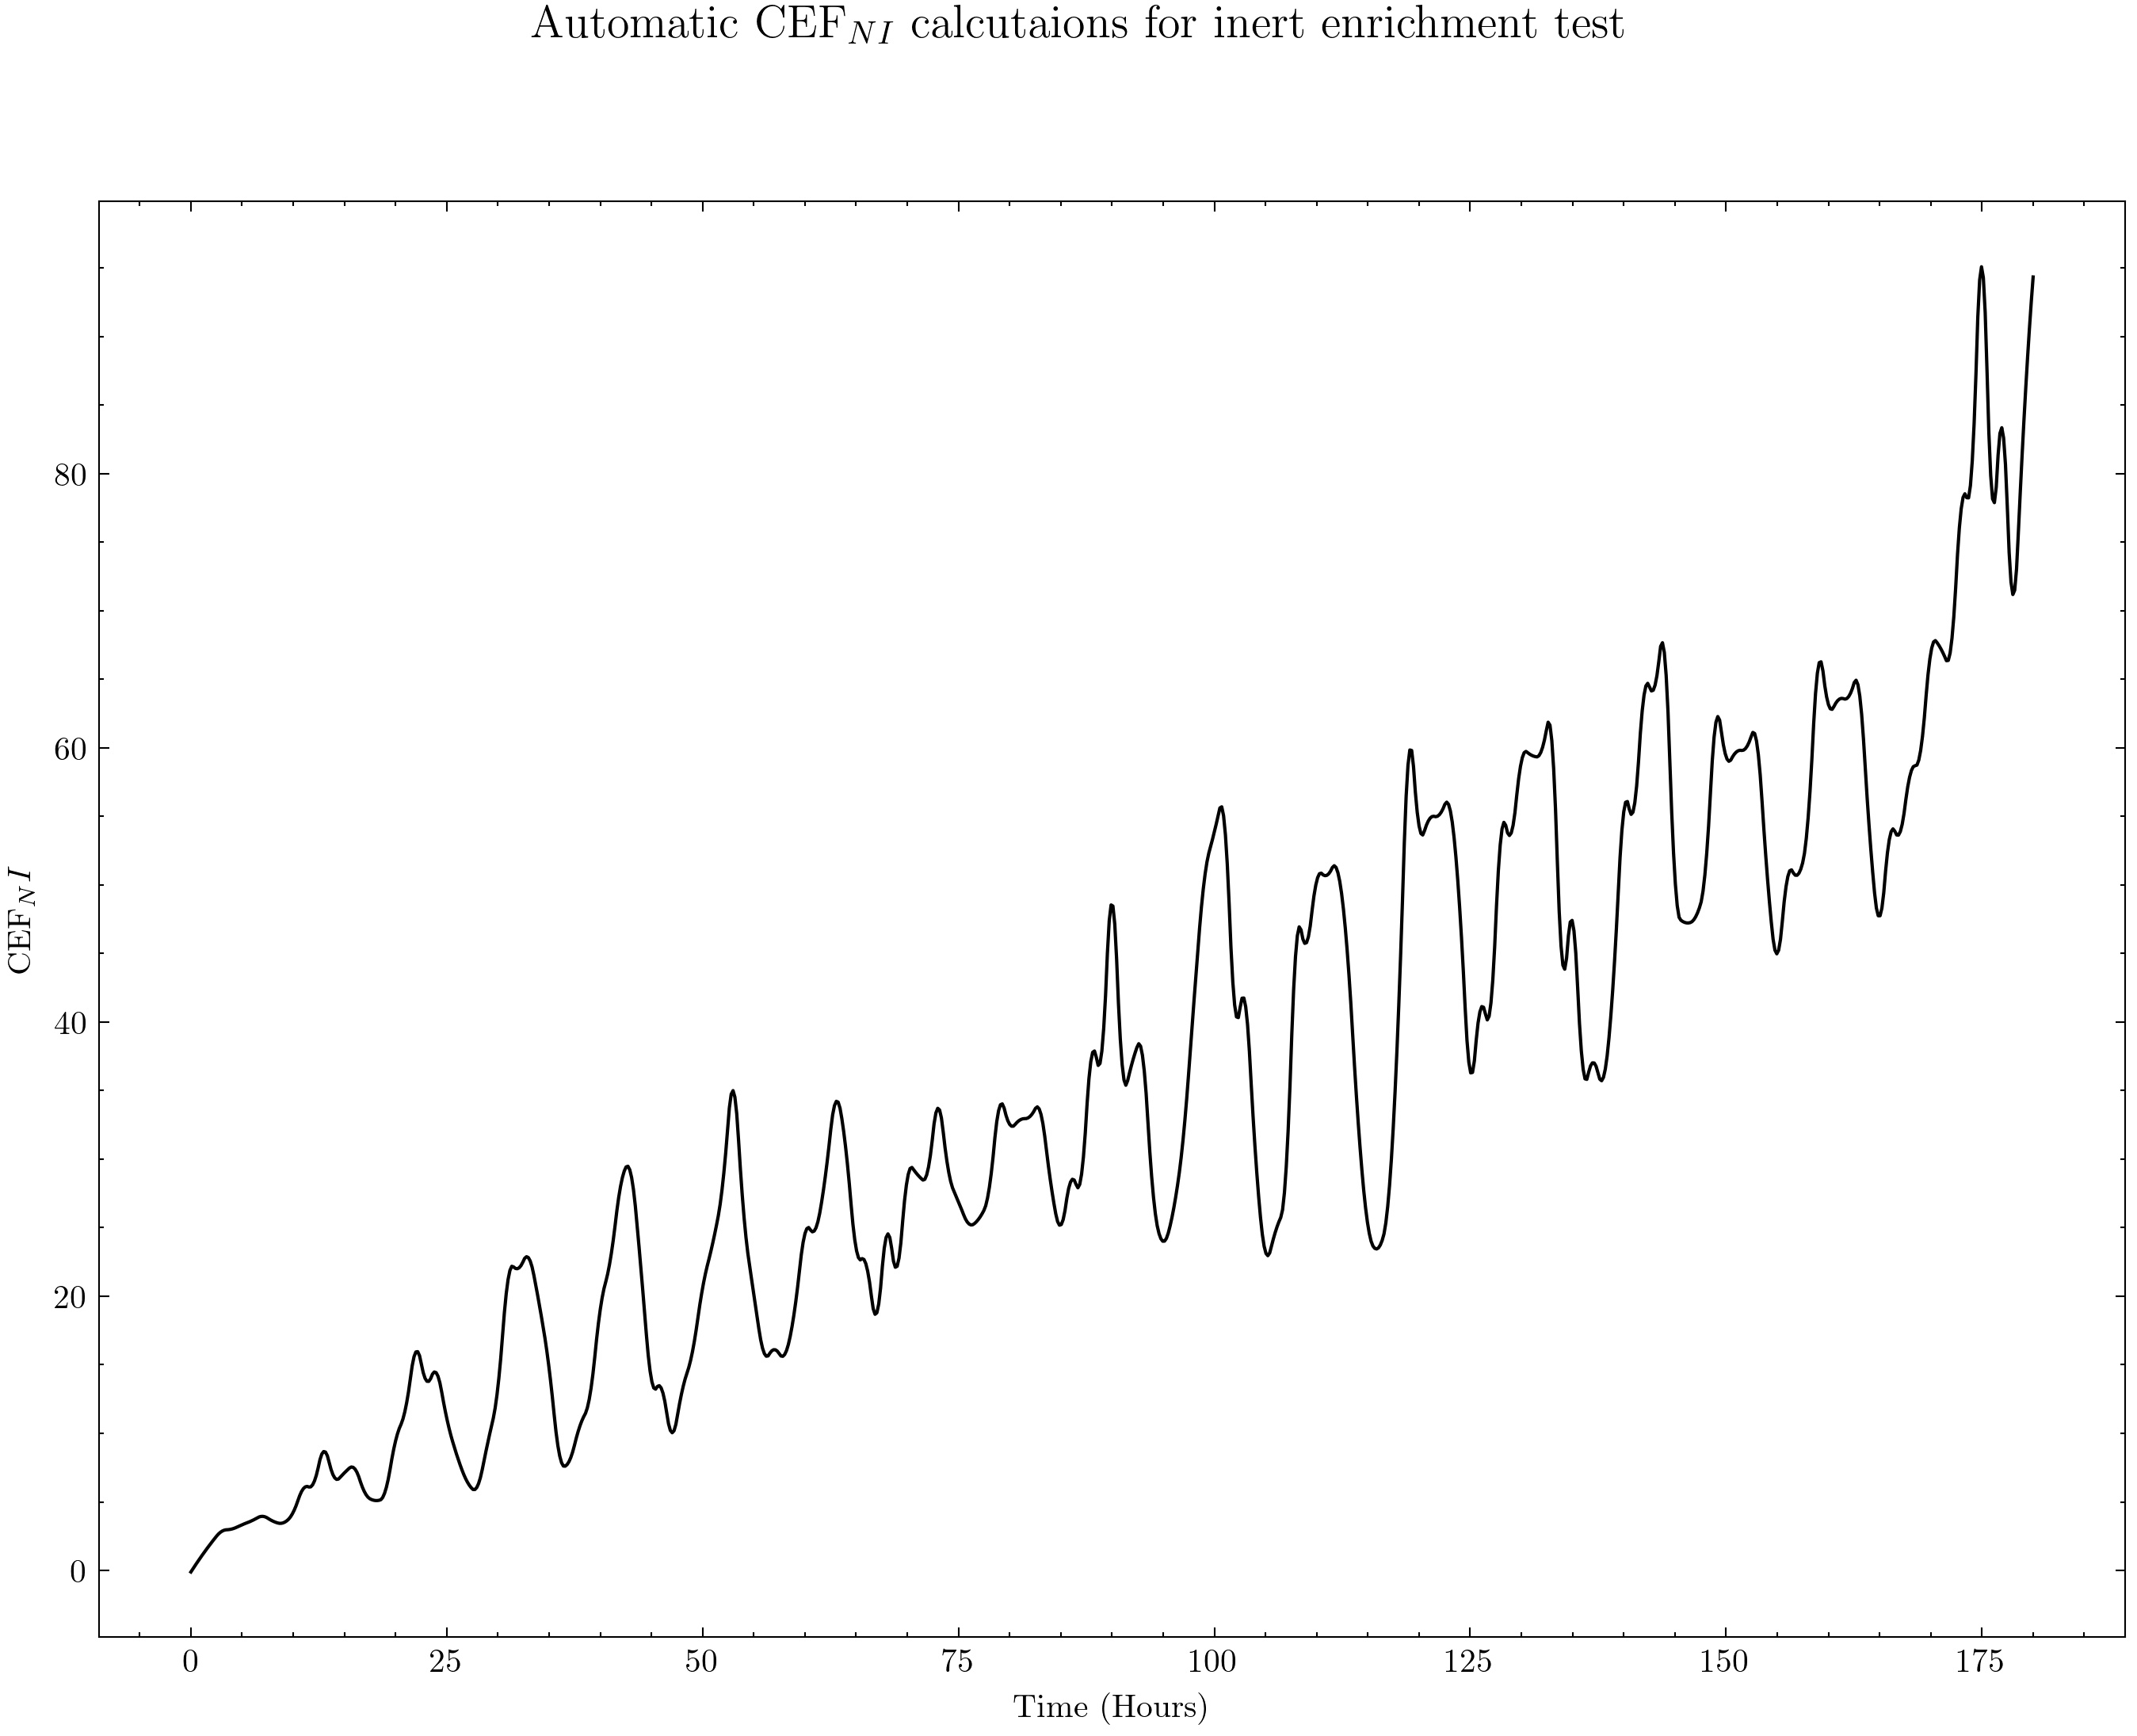
\includegraphics[width=0.9\linewidth, keepaspectratio]{/Users/marc/Thesis/Chapter5/inertenrich.jpg}
        \caption{$CEF_{NI}$ over the 180 hour enrichment of the inert hydrogen sample shown in table \ref{inert}}
        \label{GCNI}
    \end{figure}
\end{landscape}

Once the enrichment was complete, the system was isolated and left to cool. The transportable unit was then disconnected and it's composition measured and compared with it's original composition. Results were compared to nitrogen samples containing 251 nmol/mol, 500.77 nmol/mol, 1064 nmol/mol, 1437.37 nmol/mol using a derived calibration curve to account for non-linearity of the detector. The GC-PDHID data is shown in figure \ref{GCinert}. This analysis found that the enriched gas contained 514.62 ± 52 \textmu mol/mol of krypton and 570 ± 60 \textmu mol/mol of Nitrogen. Calculating the $CEF_T$ using the tracer enrichment method gave a value of 86 ± 9 . 

The calculation using $CEF_{NI}$ gave an initial Nitrogen concentration of 6.11 \textmu mol/mol (-7\%)N\textsubscript{2}. The tracer enrichment method calculated a value of 6.48 \textmu mol/mol (-1.7\%) further showing that the tracer enrichment method provides a more accurate result. 

\begin{figure}[H]
    \centering
    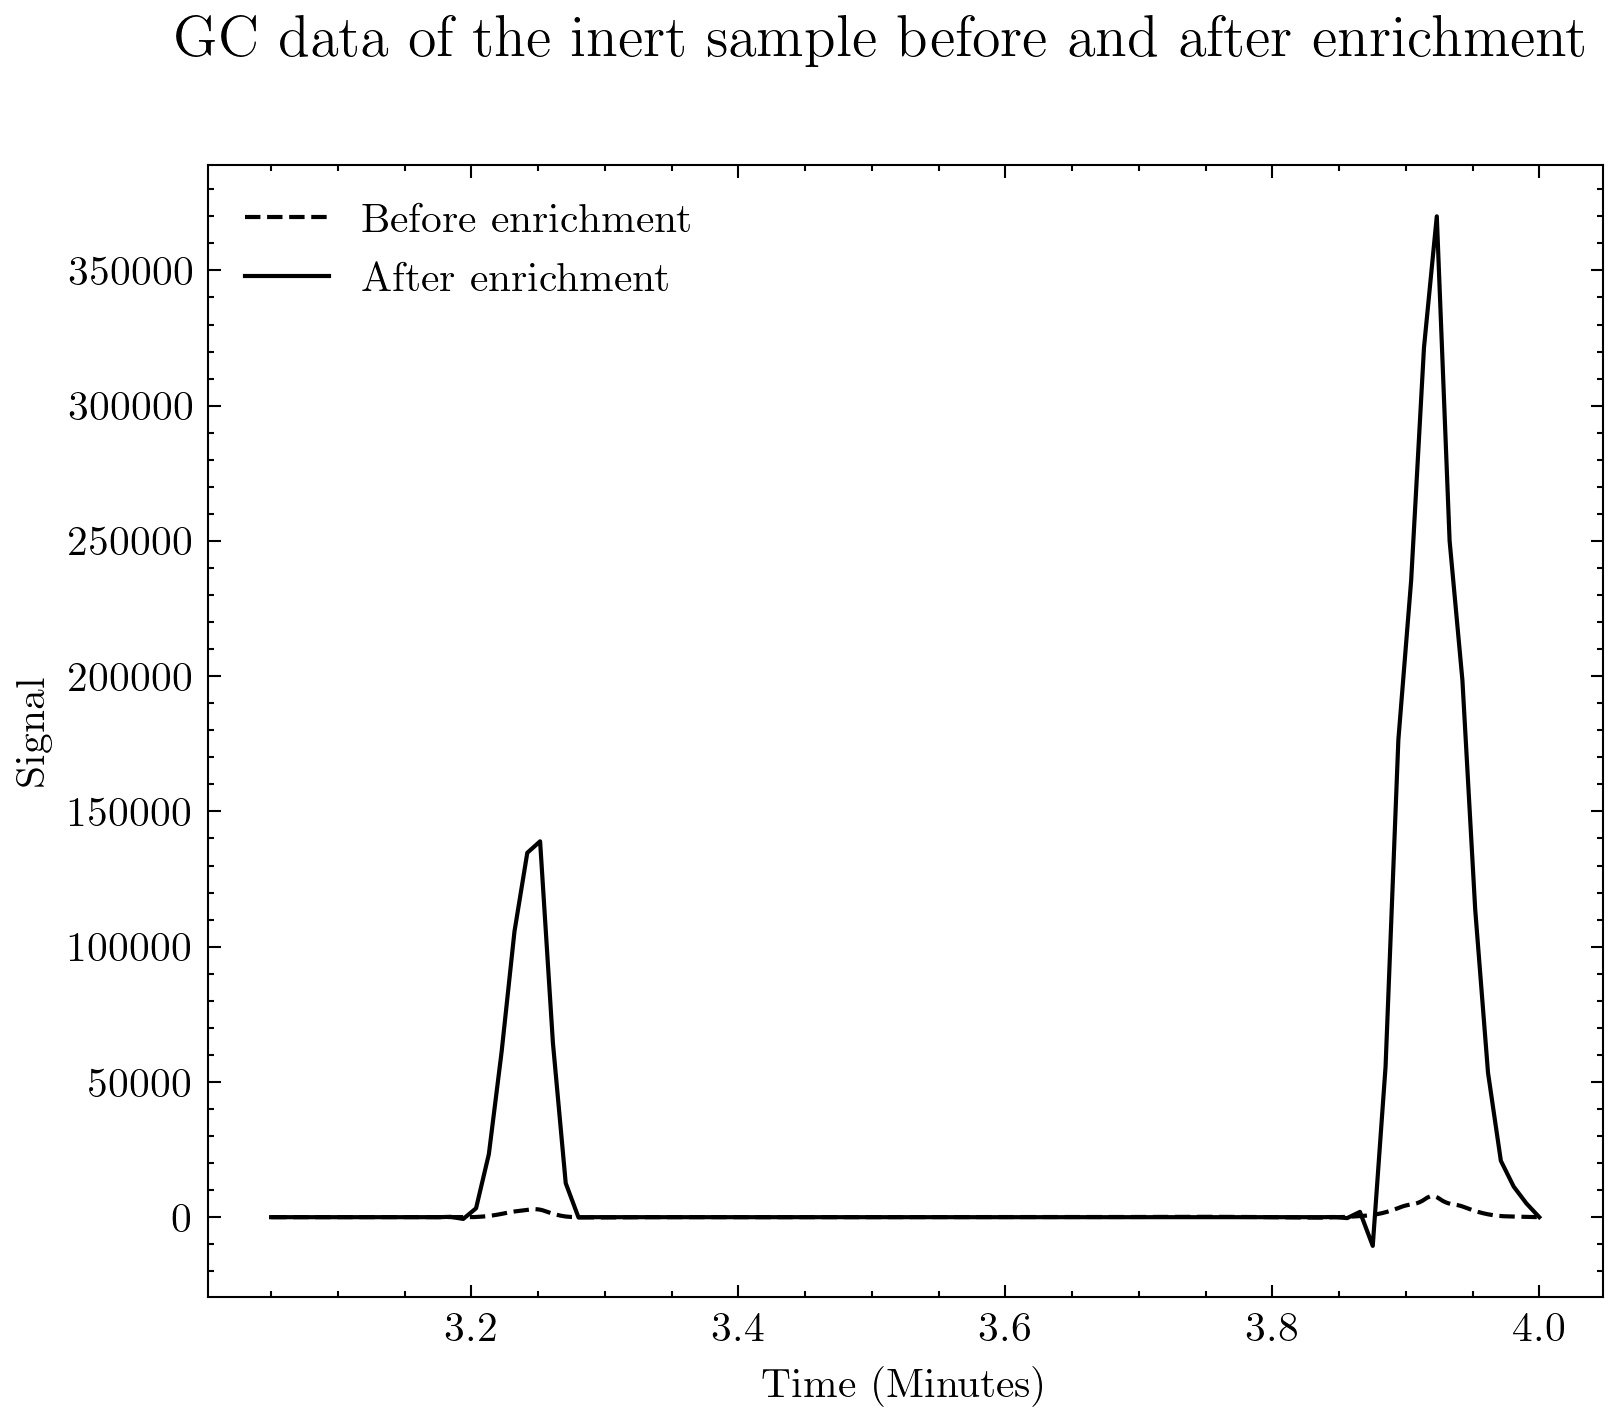
\includegraphics[width=\linewidth, keepaspectratio]{/Users/marc/Thesis/Chapter5/inertgc.jpg}
    \caption{GC-PDHID data of the inert sample both before and after enrichment with N\textsubscript{2} peaks shown at Time=3.25, and Kr peaks shown at Time=3.92}
    \label{GCinert}
\end{figure}

\subsection{Sulphur containing compounds}
The sulphur containing samples were tested using the same set up as section \ref{inertsec}, with the commercial PdAgAu membrane, and the PdCuZr alloy manufactured in chapter \label{proc-testingchapref}. The $CEF_{NI}$ values calculated in line for the experiment are shown in figure \ref{GCSULF}.

The commercial membrane saw the same dramatic drop in permeability as observed in chapter \ref{proc-testingchapref}. The experiment continued however it became clear that the permeability of the commercial membrane was dropping as the experiment went on, eventually becoming inactive to hydrogen permeability. The experiment was stopped. Upon analysis of the gas remaining within the enrichment vessel it was noted that the composition had significantly changed. This is shown in figure \ref{GCSULFCOMM}. The OCS, t-BuSH, THT and CS\textsubscript{2} in the gas mixture had reacted with the hydrogen to form H\textsubscript{2}S. While this would not effect the results of analysis much, sine the ISO 14687-2 standard does not give a maximum level of a specific sulphur containing compound, only the total concentration, OCS, THT, T-BuSH and CS\textsubscript{2} all contain carbon molecules. The result of this could be the formation of hydrocarbons, CO, or solid carbon on the surface of the membrane. In the case of carbon deposition, this would explain the complete deactivation of the membrane as discussed previously in section \ref{lit-pdreview}. In order to prevent this the exact reactions should be determined and process parameters further optimised to inhibit them from taking place. 

\begin{figure}[H]
    \centering
    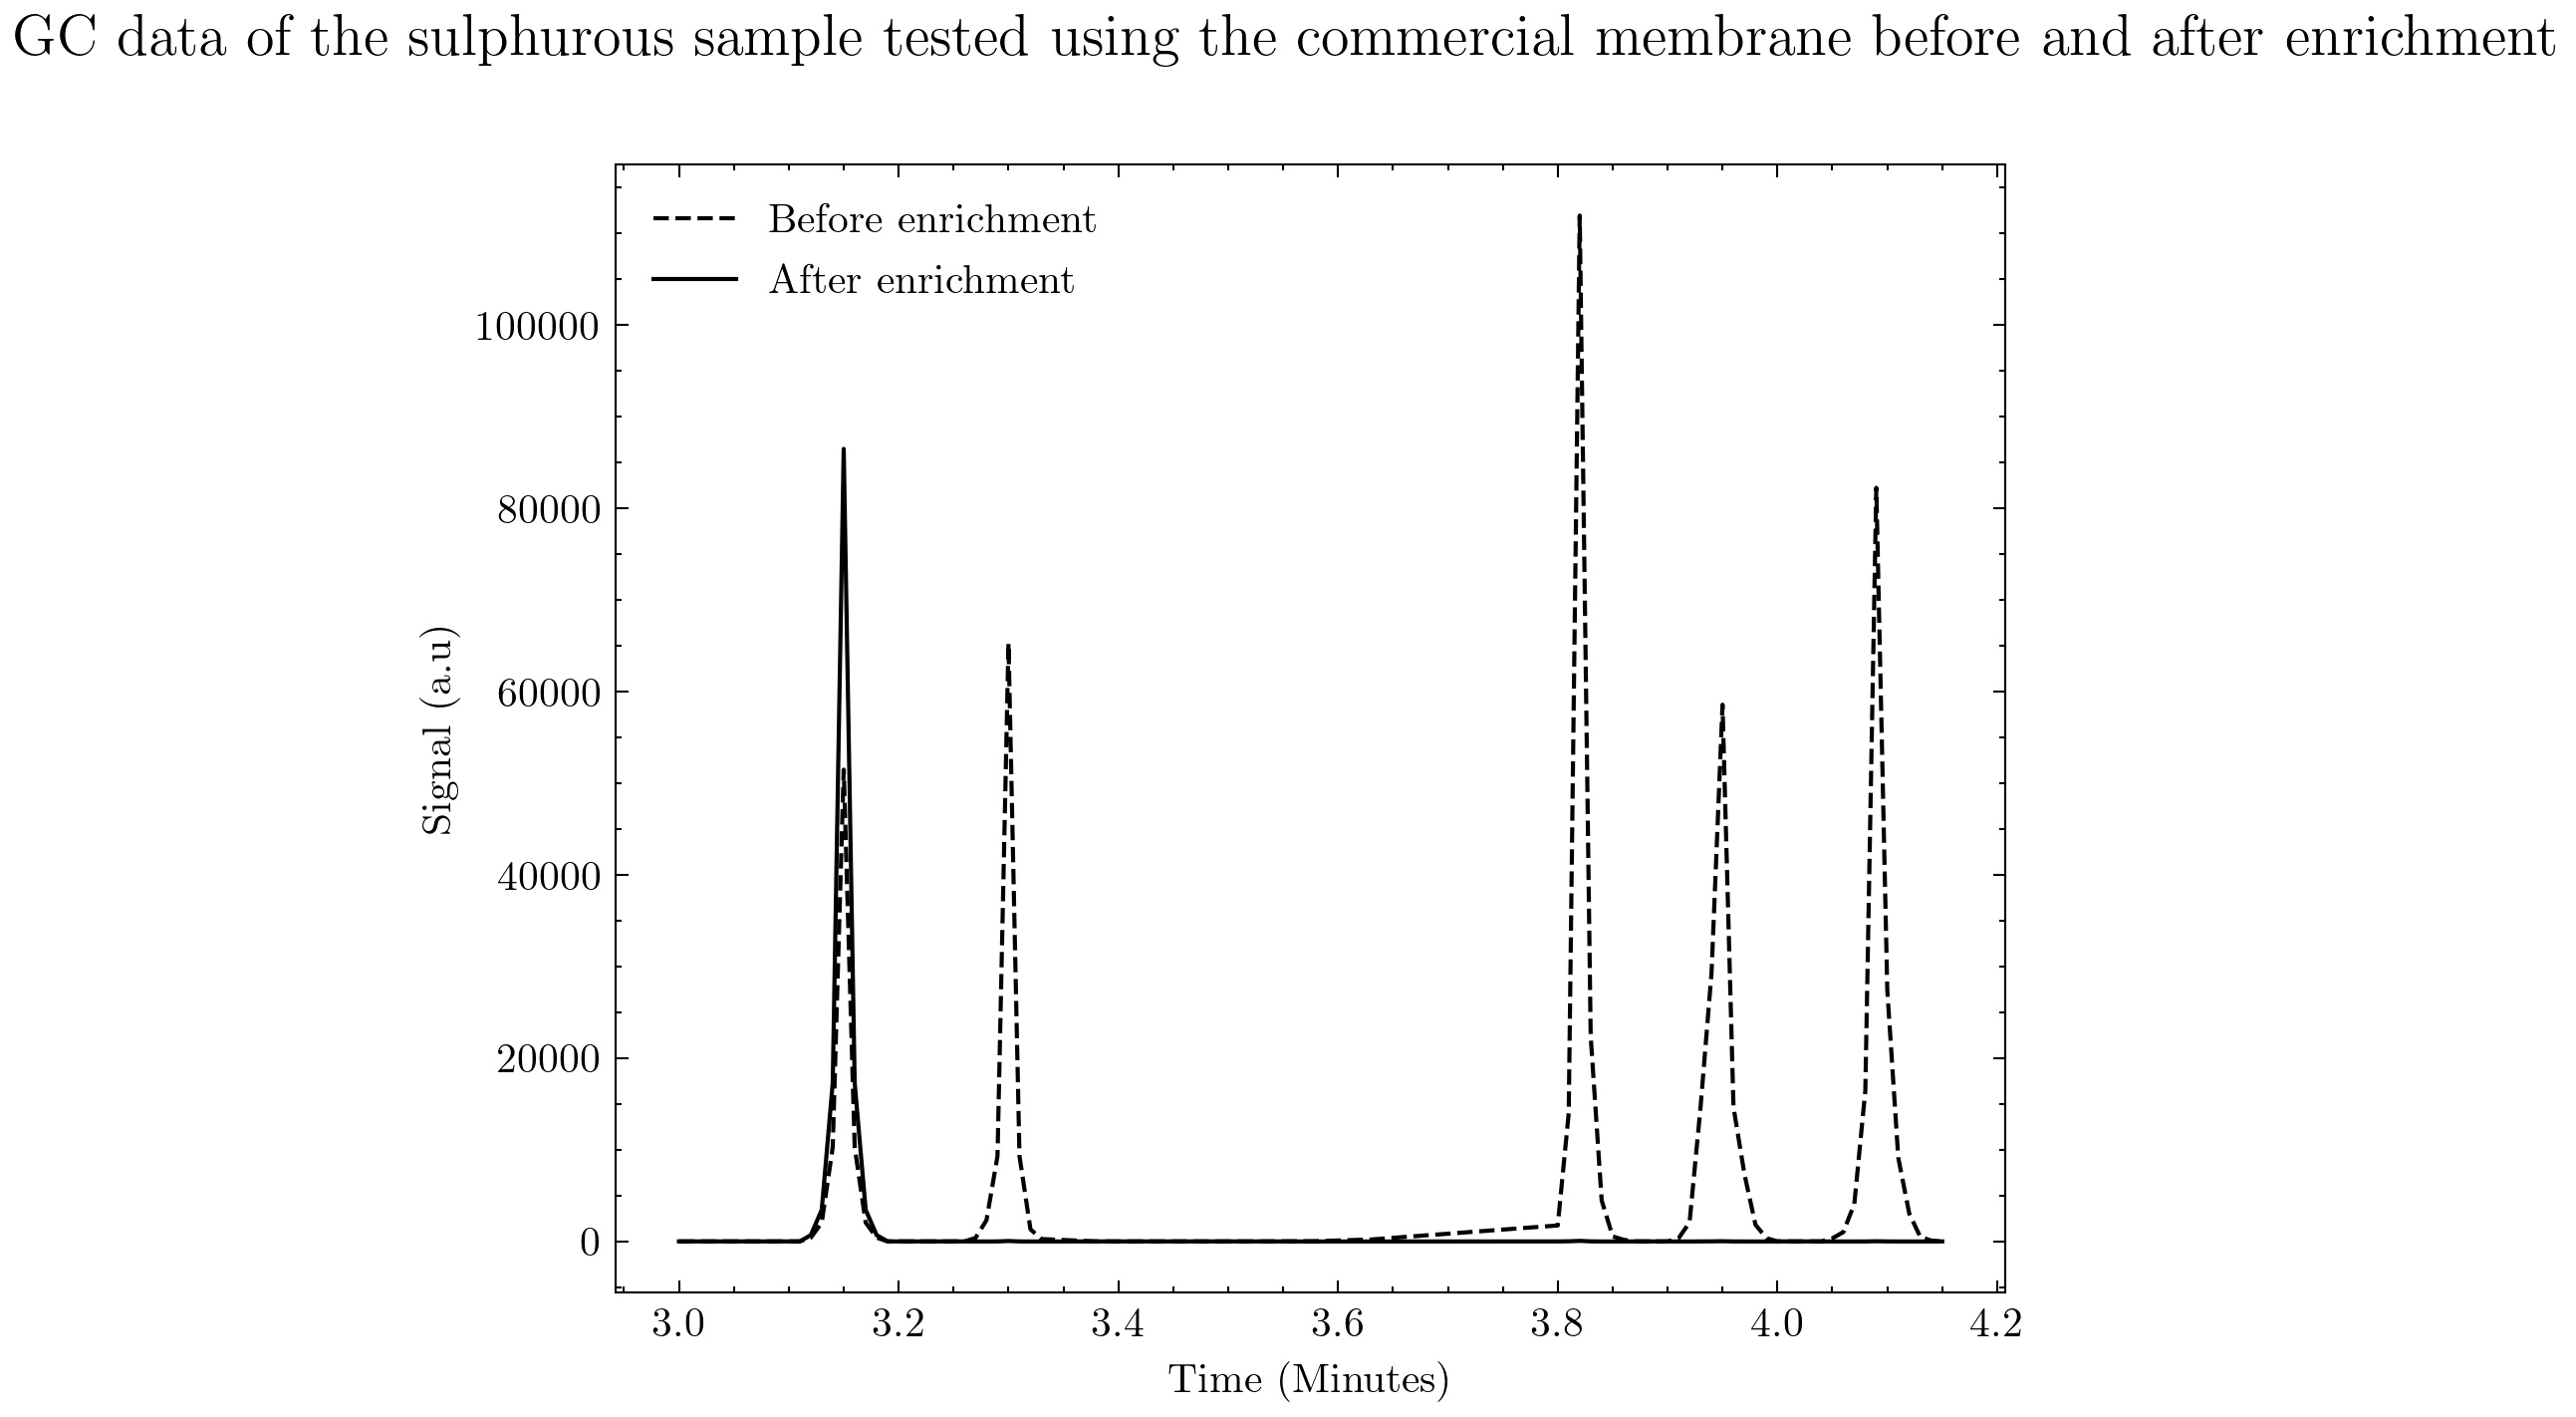
\includegraphics[width=\linewidth, keepaspectratio]{/Users/marc/Thesis/Chapter5/sulfcomgc.jpg}
    \caption{GC-SCD data of the sulphurous sample both before and after enrichment with commercial membrane}
    \label{GCSULFCOMM}
\end{figure}

The PdCuZr membrane was tested twice, with both runs ending in failure due to delamination of the membrane after a number of temperature cycles. On the second attempt the heating ramp was lowered to 1 \textdegree C/min in order to put less thermal strain on the membrane. This resulted in the membrane lasting one extra temperature cycle, however made no lasting difference to the result. The reason for this is likely to be the combined force of the extra pressure in the enrichment vessel durting heating, and the multiple heating cooling cycles used over the course of the experiment causing the mismatch between the thermal expansion coefficient betwen the membrane and support to result in membrane failure. 

Since all enrichment experiments failed for the sulphur sample a comparison of the enrichment factors in sulphur containing atmospheres cannot be performed. 

\begin{landscape}
    \begin{figure}
        \centering
        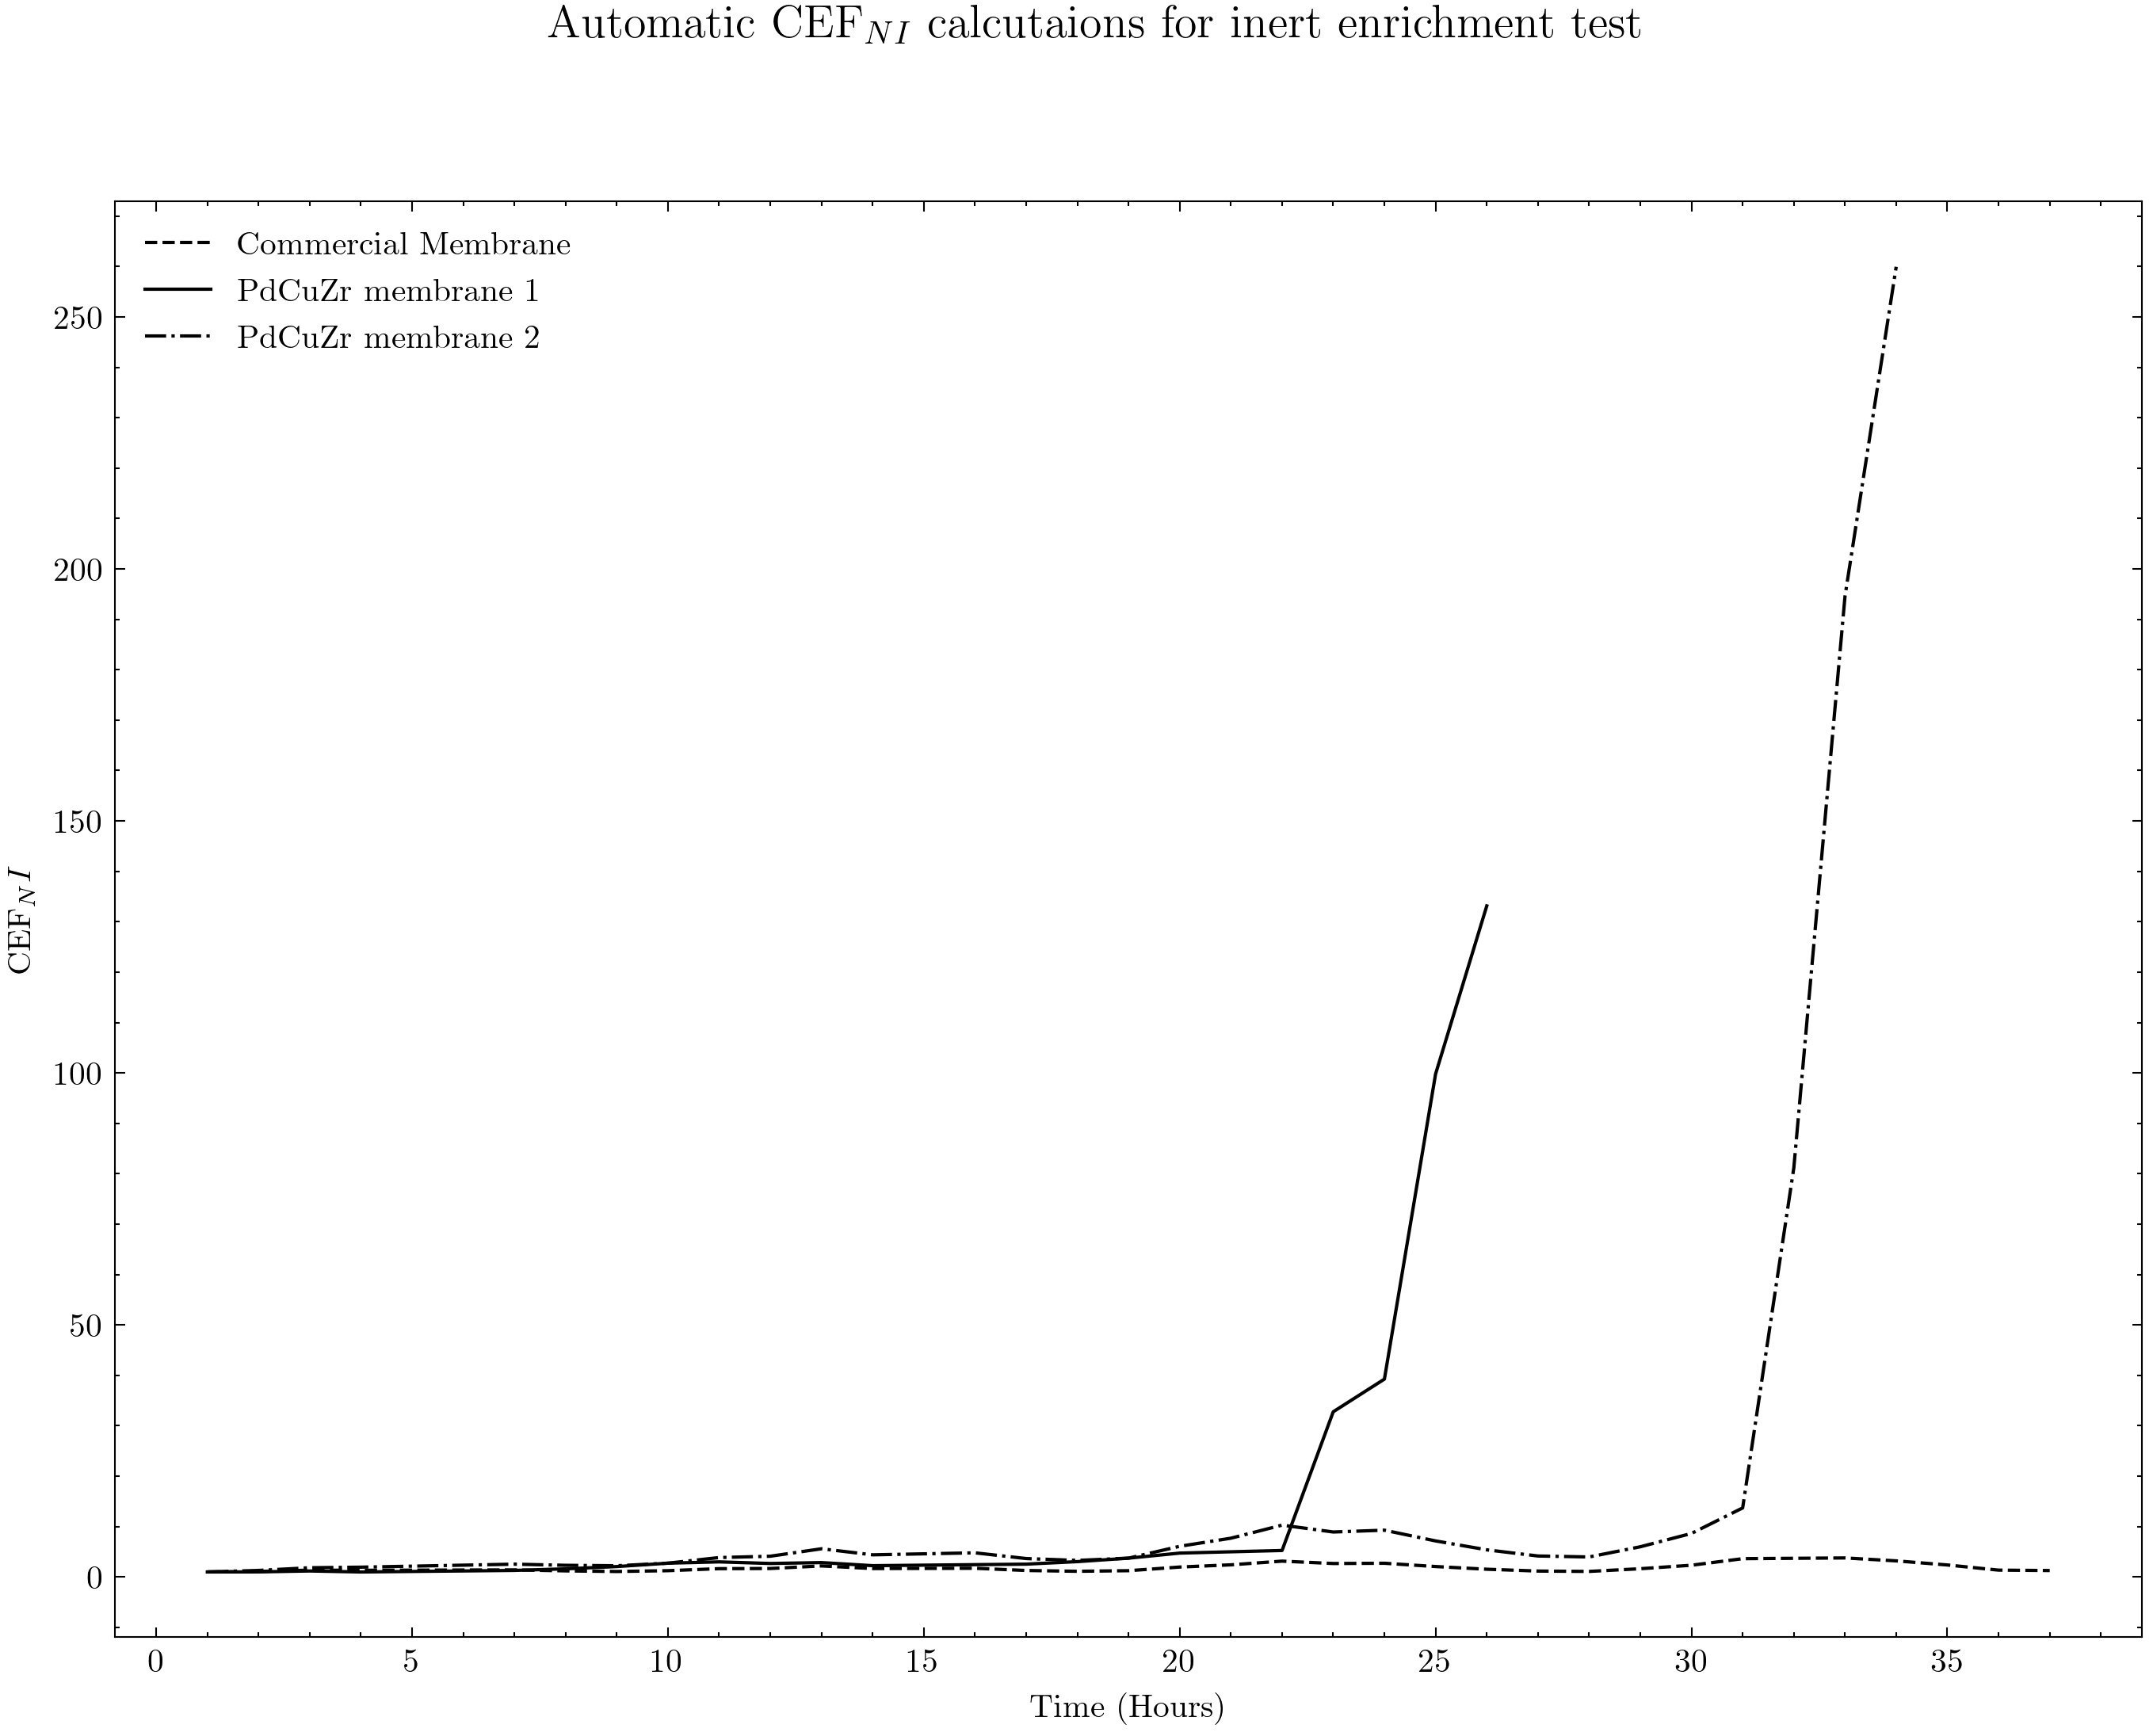
\includegraphics[width=0.9\linewidth, keepaspectratio]{/Users/marc/Thesis/Chapter5/sulfenrichni.jpg}
        \caption{$CEF_{NI}$ over the 40 hour enrichment of the sulphurous hydrogen sample shown in table \ref{exp-sulf}}
        \label{GCSULF}
    \end{figure}
\end{landscape}

\subsection{HRS sample}
The sample taken from the hydrogen refuelling station spiked with krypton as described in \ref{kryptonspike} was enriched using the commercial PdAuAg membrane as this was the only composition able to withstand the conditions required for enrichment. The enrichment was performed over 120 hours. Initial analysis showed that the krypton concentration in the sample before enrichment was 80 \textmu mol/mol and that nitrogen was present in the sample likely due to dead volume within the H\textsubscript{2} qualitizer. The CEF\textsubscript{NI} over the course of the experiment is shown in figure \ref{GCHRS} and predicted that the sample was enriched 55.36 ± 3.4 times using the non-ideal gas law method.

\begin{landscape}
    \begin{figure}
        \centering
        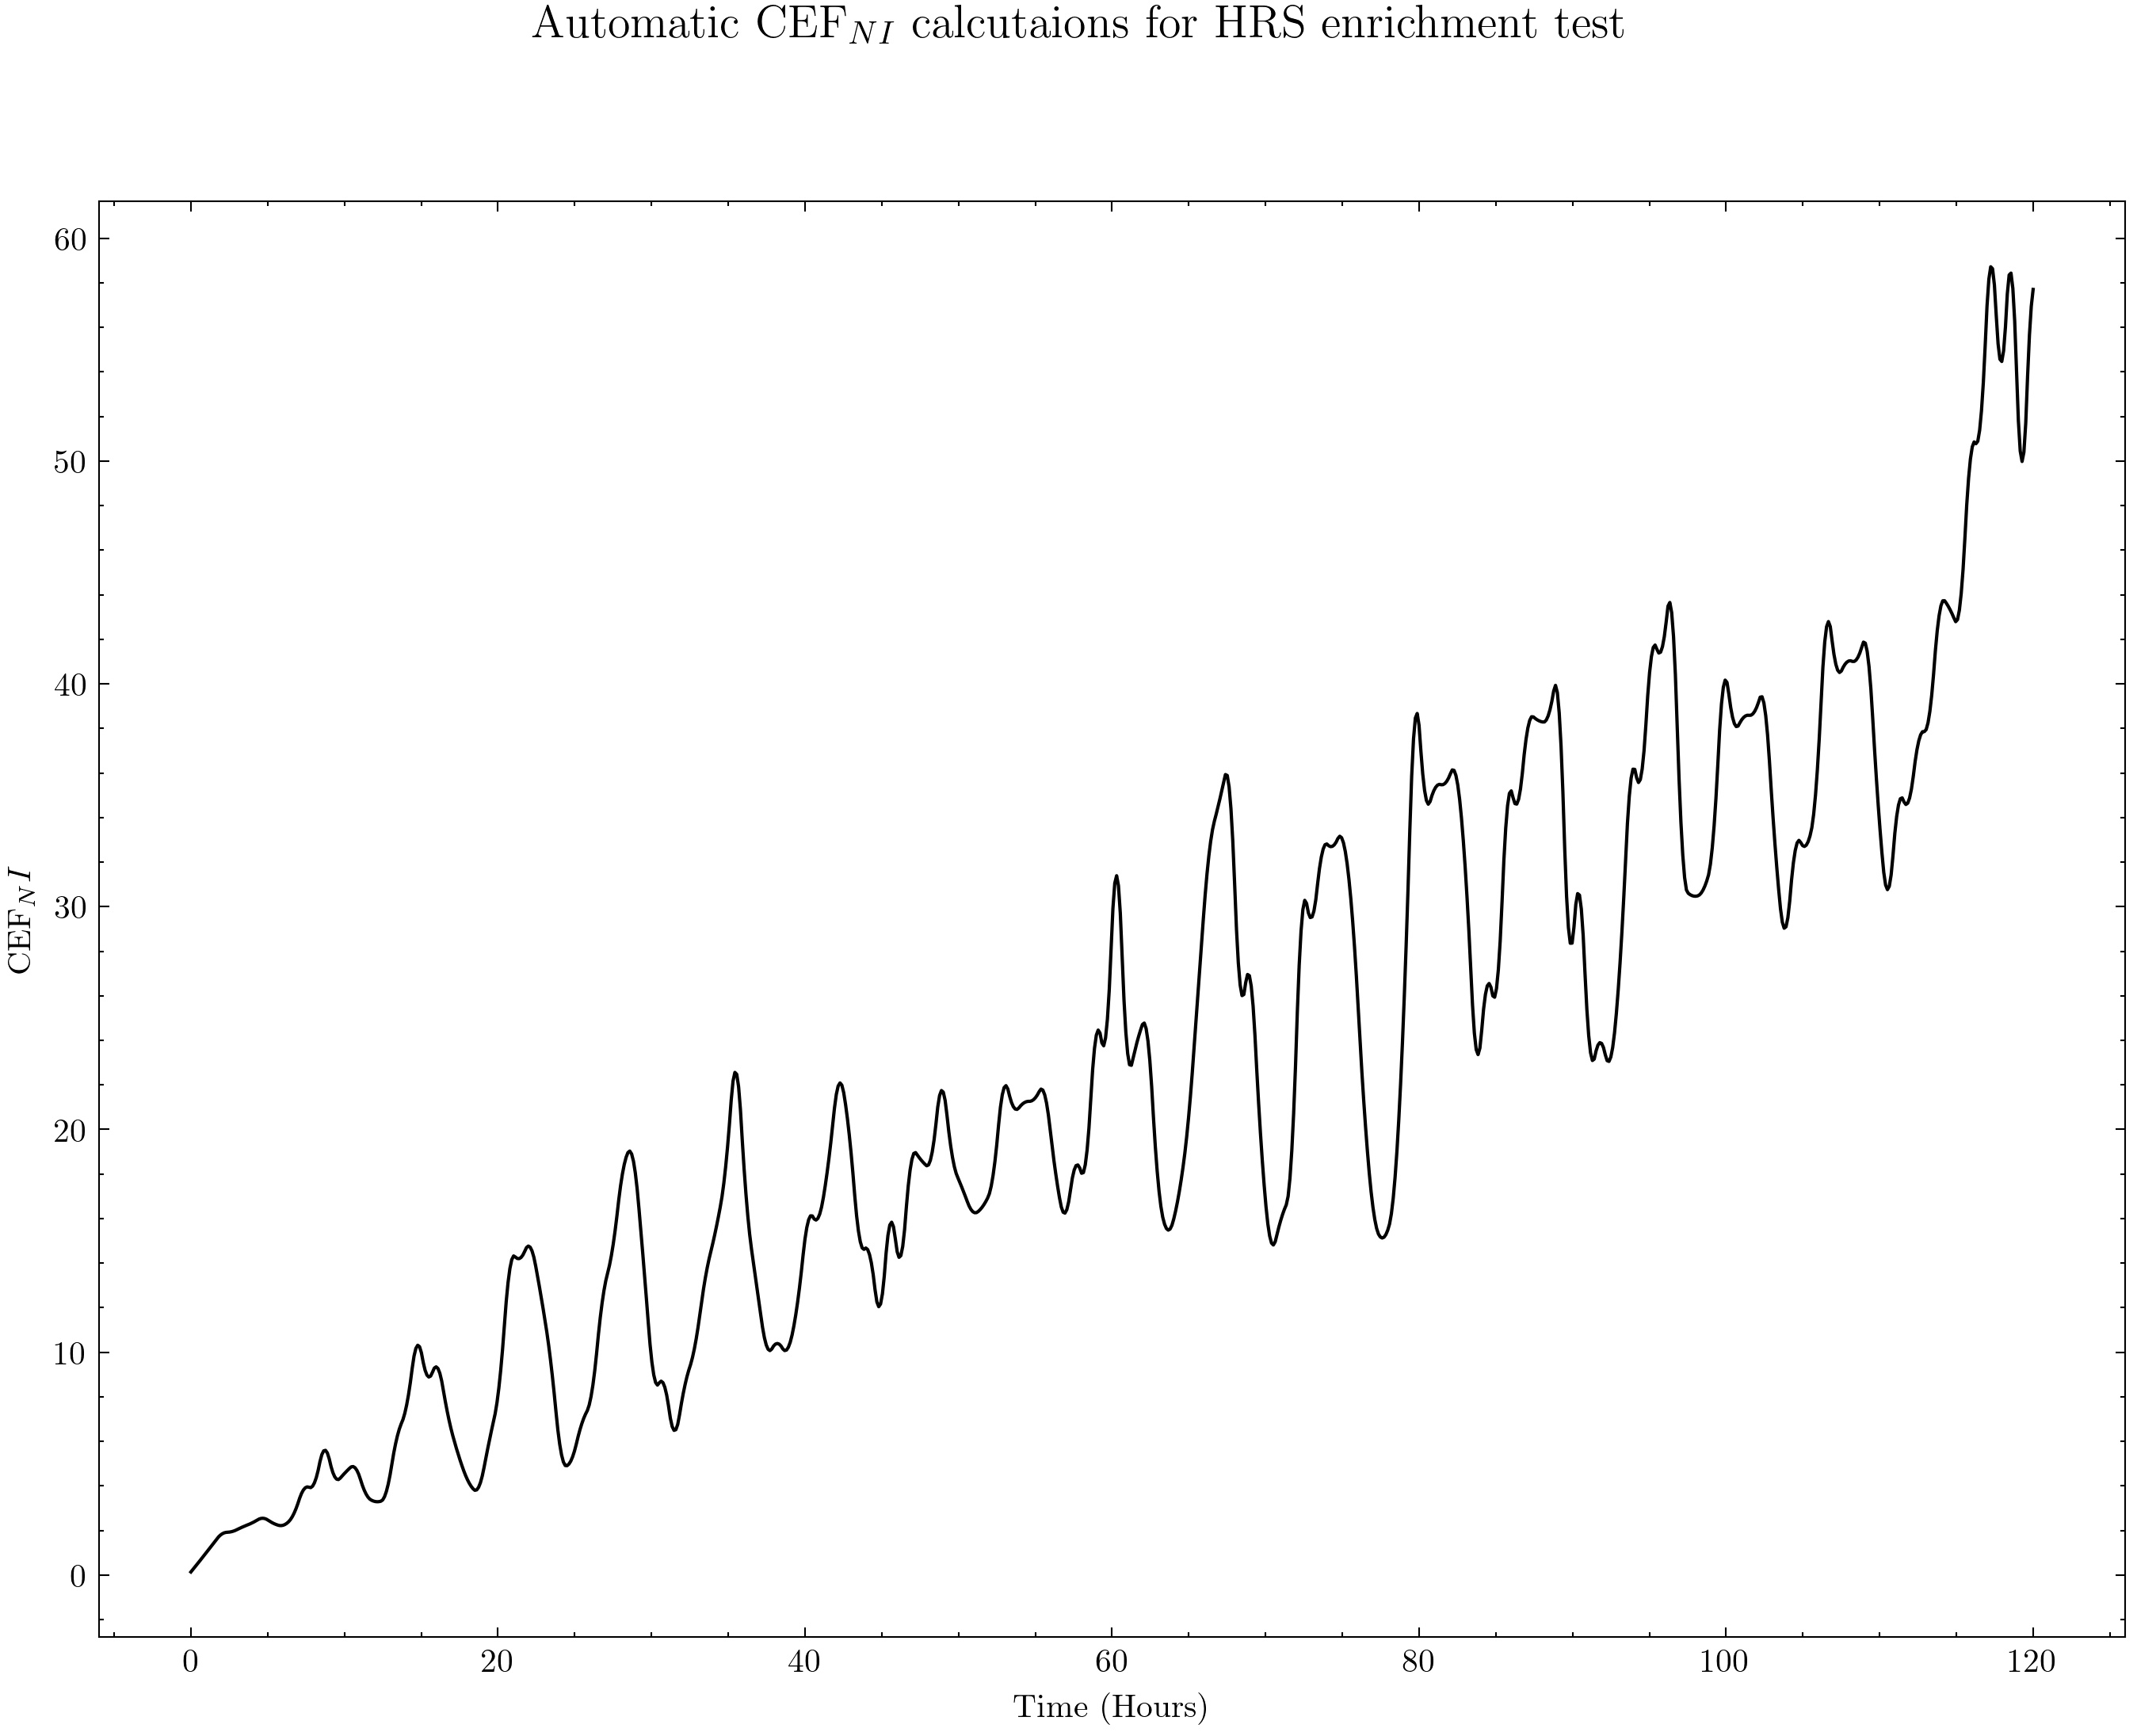
\includegraphics[width=0.9\linewidth, keepaspectratio]{/Users/marc/Thesis/Chapter5/hrsenrichni.jpg}
        \caption{$CEF_{NI}$ over the 120 hour enrichment of the HRS hydrogen sample}
        \label{GCHRS}
    \end{figure}
\end{landscape}

The sample was enriched to an enrichment factor of 41.76 ± 2.3 as shown by the increase of krypton and nitrogen concentrations shown in figure \ref{HRSGCENRICH}. These peaks corresponded to concentrations of 3374 ± 32 \textmu mol/mol of krypton and 957 ± 10.6 \textmu mol/mol of Nitrogen respectivley. Using the tracer enrichment factor this corresponds to an initial concentration  of 22.91 ± 3.2  \textmu mol/mol of Nitrogen  in the hydrogen sample. The results in the enriched sample also show a new peak at 2.4 minutes which corresponds to Argon, thereby proving that the method can be used to quantify impurities which were below the limit of detection of the detector in the initial sample. Due to the small size of the peak, quantifying the concentration was difficult and a higher enrichment factor would be required to accurately determine this. Unfortunately due to interrruptions from COVID-19 adequate time was not avaliable to perform this test. 

\begin{figure}[H]
    \centering
    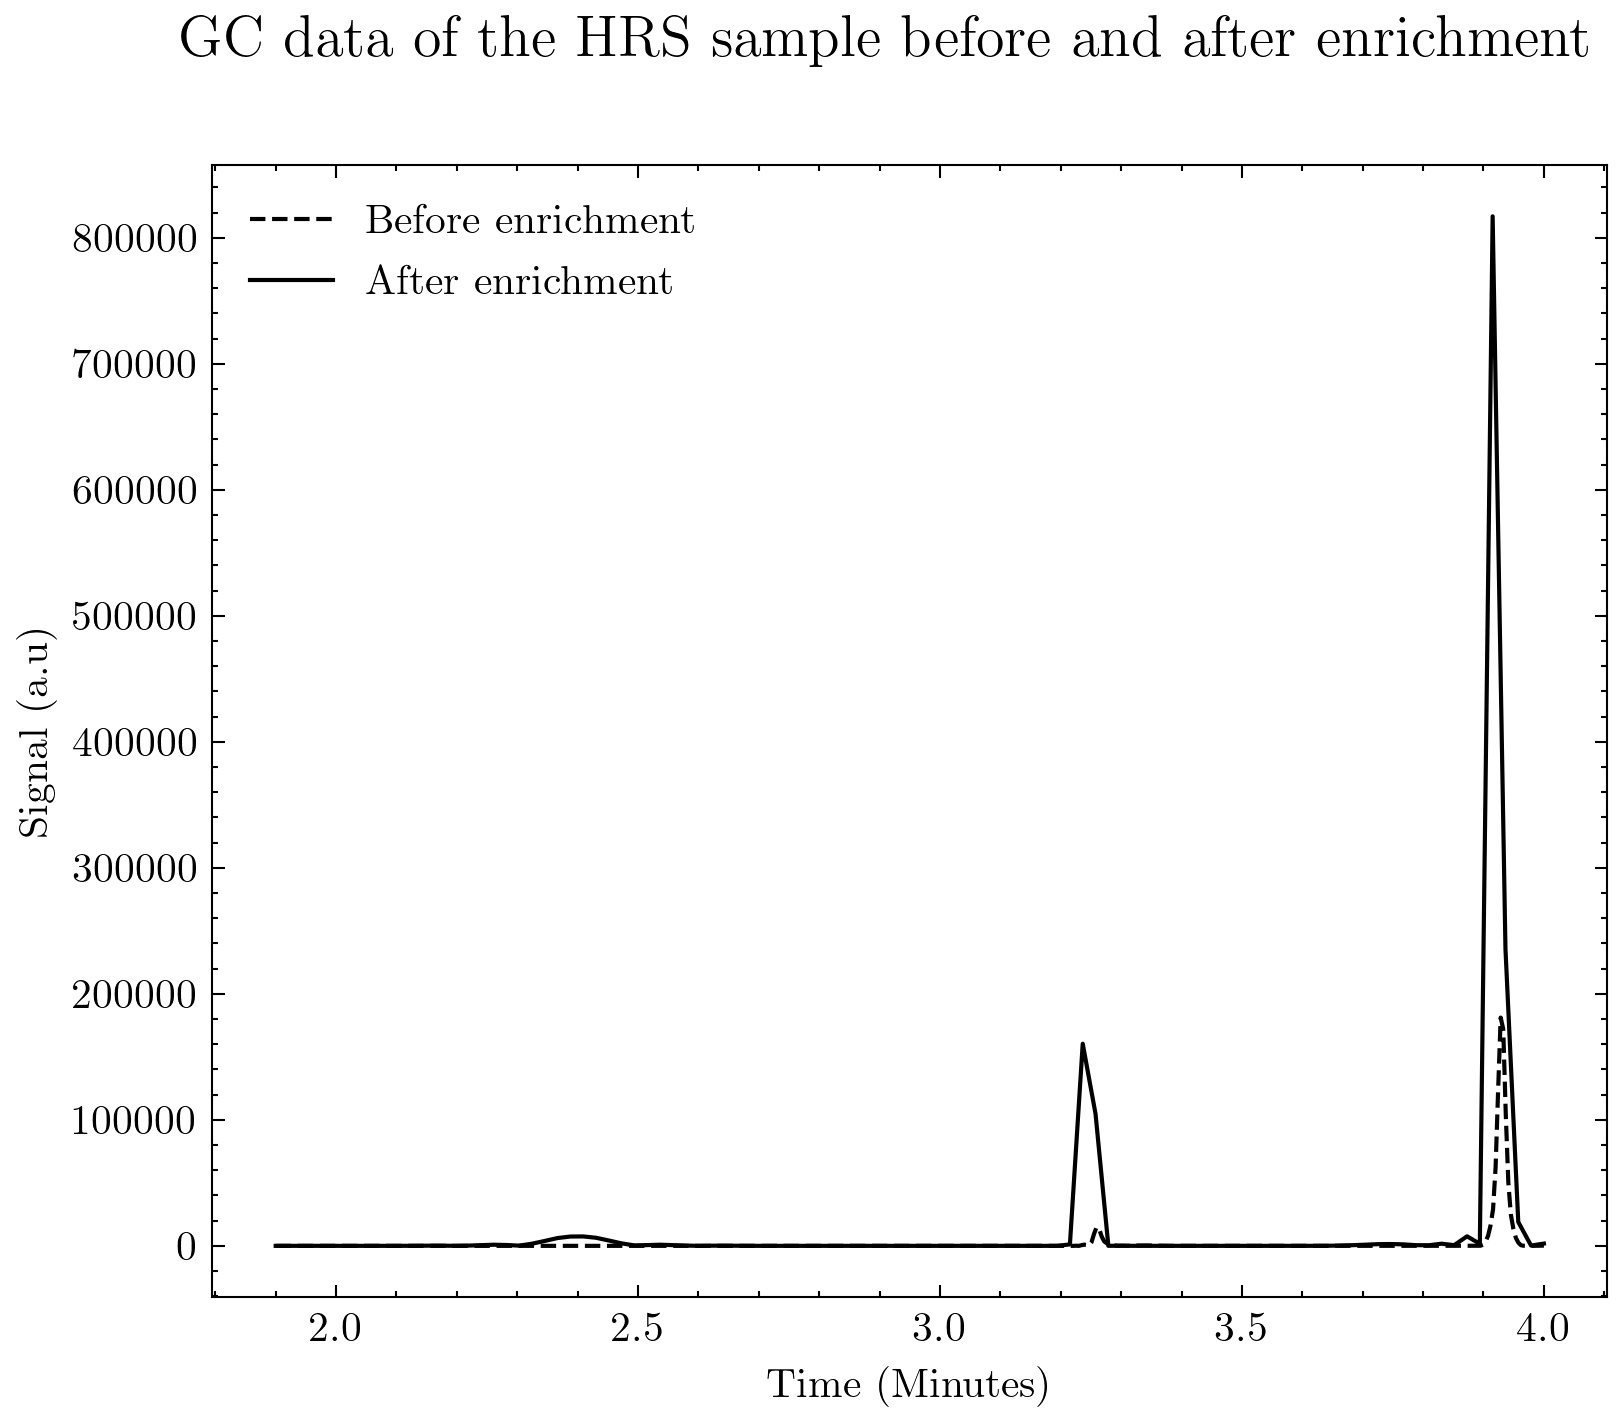
\includegraphics[width=\linewidth, keepaspectratio]{/Users/marc/Thesis/Chapter5/hrsgc.jpg}
    \caption{GC-PDHID data of the HRS sample both before and after enrichment with commercial membrane}
    \label{HRSGCENRICH}
\end{figure}

\section{Conclusion}
The new enrichment device was tested using 3 hydrogen samples, a sample containing only inert impurities in order to test the device functions as required, a sulphur containing sample to test how the PdCuZr membrane identified as the best membrane in chapter \label{proc-testingchapref}, and a sample taken from a hydrogen refuelling station. The inert sample was successsfully enriched to 50x and using the tracer enrichment method using krypton the initial concentration of nitrogen was calculated to within 2\% of it's original value. 

The sulphur tests resulted in failure of all membranes used. For the commercial membrane this was due to high reactivity with the sulphur compounds which was also identified in chapter 5. For the PdCuZr membrane this was due to material instability and further work is required to manufacture the ceramic supported membrane to be able to withstand temperature cycling. 

For the first time enrichment was performed on a real sample from a hydrogen refuelling station, proving both that the method is viable for analysis of real world hydrogen samples, and the protocol for spiking a hydrogen sample with krypton gas is approptiate. The sample was enriched 41 times and was able to accurately determine that the concentration of nitrogen in the sample before enrichment was 22.91 \textmu mol/mol. Enrichment also revealed the presence of Argon in the sample, which would not have been present in the analysis otherwise, further proving that the technique can provide a more accurate composition analysis of fuel grade hydrogen, past what is possible with commercial analysers.


\chapter{Conclusions and future work}

\section{Membranes for hydrogen separation}
\subsection{DFT for screening impurity resistant alloys}\label{simconc}
This thesis presented a methodology for fast screening of palladium alloy membrane compositions for resistence of impurities. The simulations involving sulphur samples were relatively accurate, and were able to successfully predict which membranes would perform the best when tested in chapter 5. The model however broke down for other impurities and this is due to the fact that the chosen simulation method is not accurate for weak interactions. \cite{dftbook1} Further development of the models should be performed in order to accurately predict the impact of these impurities. The model can also be expanded to predict the solubility of hydrogen within the palladium alloy membranes by combining monte carlo simulation techniques with cluster expansion simulations as has been performed by Scholl et al. \cite{SHOLL2007462} Future work could take combine these simulation methods to predict everything from the impurity interactions, to permeability and performance of the membranes. If such a system was developed it could greatly reduce the time taken to discover new alloy compositions. 

There is also scope for testing more membrane compositions. This thesis tested a limited number of alloy composition due to lack of computing power and time available. With HPC networks becoming more and more available \cite{morgan_burt_feldman_2020} a great number of alloys can be simulated quickly, allowing bespoke membrane compositions to be potentially found for any application. 


\subsection{Use for dense metal membranes in the hydrogen economy}
In this work we presented a use case for dense metal membranes as a material to perform hydrogen impurity enrichment to measure ISO 14687-2 impurities. As the hydrogen economy grows there will be other potential uses for such technology. 

There are already examples of industry capturing waste hydrogen from their processes and using it as a power source either through a fuel cell, or other means.\cite{doi:10.1177/0144598719839767} It is estimated that there are 100,000MW of waste hydrogen produced each year and therefore could result in a meaningful resource. \cite{cox} As more processes turn to this there is potential for a highly personalised market for dense metal membranes. Dense metal membranes provide ultrapure hydrogen suitable for use in fuel cells, therefore protecting the investment in any new type of energy utilization technology and this will become especially true as the cost of such membranes decreases through the development of stable ceramic supported membranes.

If combined with the simulation research discussed in section \ref{simconc} there could be potential for an highly linked membrane ecosystem. Where a plant owner can define the requirements for their hydrogen separation process, the optimal membrane can be found by a computational research provider, and finally manufactured into a module. This process is visualised in figure \ref{manuproc}

\begin{figure}
    \centering
    
\includegraphics[width=\linewidth, keepaspectratio]{/Users/marc/Thesis/Chapter6/manuproc.png}
    \caption{Theoretical manufacturing process for a bespoke dense metal membrane with optimal composition calculated by a research provider, manufactured to specification, and delivered to the customer}
    \label{manuproc}
\end{figure}

Another potential use for dense metal membranes is in a potential hydrogen grid system. Projects such as HyGrid \cite{hygrid} aim to use the existing natural gas network in Europe as a storage medium for the hydrogenm economy, mixing hydrogen with natural gas to improve it's energy density and reduce the carbon footprint of the natural gas network. In addition to this there are several companies now offering hydrogen CHP systems for use in homes, which are powered using a fuel cell, to provide thermal energy for households.\cite{giacomini} There may soon be a need for a source of ultrapure hydrogen. Palladium membranes could be used to provide this, separating the hydrogen out from the natural gas network at the point of use. The challenge with this is that there are a number of impurities present in the natural gas network, potentially varying even by region. There is an opportunity to develop bespoke membranes for such a purpose using the system described in figure \ref{manuproc}.

Ultimately most large scale hydrogen production processes will continue to use polymer membranes or PSA to provide purified hydrogen, however this thesis proves that there are a number of niche applications where palladium membranes could be used in the future hydrogen economy. 

\subsubsection*{Ceramic supported dense metal membranes}
This work used YSZ supported membranes in order to improve the flux and cost of the dense metal membranes. The techniques used in this thesis were able to deposit membranes within the range of 0.5-2 \textmu m, allowing for high flux membranes to be manufactured from materials which contain lower concentrations of palladium, and are more resistant to impurities. The module consisted of a single membrane operating in dead end, however it can be easily expanded to contain a bundle of hollow fibre membranes. Through this even extremely low flux membranes can be used as long as there are enough in the bundle to produce a flux reasonable for the chosen process. The problem that was encountered with the use of ceramic supported dense metal membranes is that they lacked stability under temperature cycling, experiencing delamination after a low number of temperature cycles. In order to be commercially viable the product must be properly optimised with a reasonable lifespan in order to provide an attractive solution to buyers. 

\section{Impurity enrichment devices}
In chapter 6 the hydrogen impurity enrichment device was greatly improved in terms of it's safety, usability and reliability. Using a comemrcial membrane it was shown to be capable of providing the concentration of nitrogen impurities in a hydrogen sample to within 2\% of it's real value, which is adequate for metrology purposes. \cite{Murugan2015} For the first time a real sample taken from a hydrogen refuelling station was also enriched and was able to quantify the level of nitrogen in the sample to 22 \textmu mol/mol. Enriching the sample was also able to show the presence of an additional impurity. Further work is required to quantify these impurities. 

\subsection{Commercialisation and optimisation}
The device manufactured in chapter 6 has already been commercialised and sold to one customer at the time of writing, with other buyers currently in the pipeline. There are however further opportunities for commercialisation that arise as the device is automated further. 

Since every hydrogen refuelling station must show that their hydrogen meets ISO 14687-2, there is potential for a hydrogen impurity device to be installed directly at every HRS to automatically provide this information. Such a system would involve four main components; a sample cylinder permentantly connected to the HRS fixed upon a mass balance, a Krypton supply connceted to the sample cylinder, the HIED, and an analyser. The process is shown in figure \ref{autoprocedure}


\begin{figure}
    \centering
    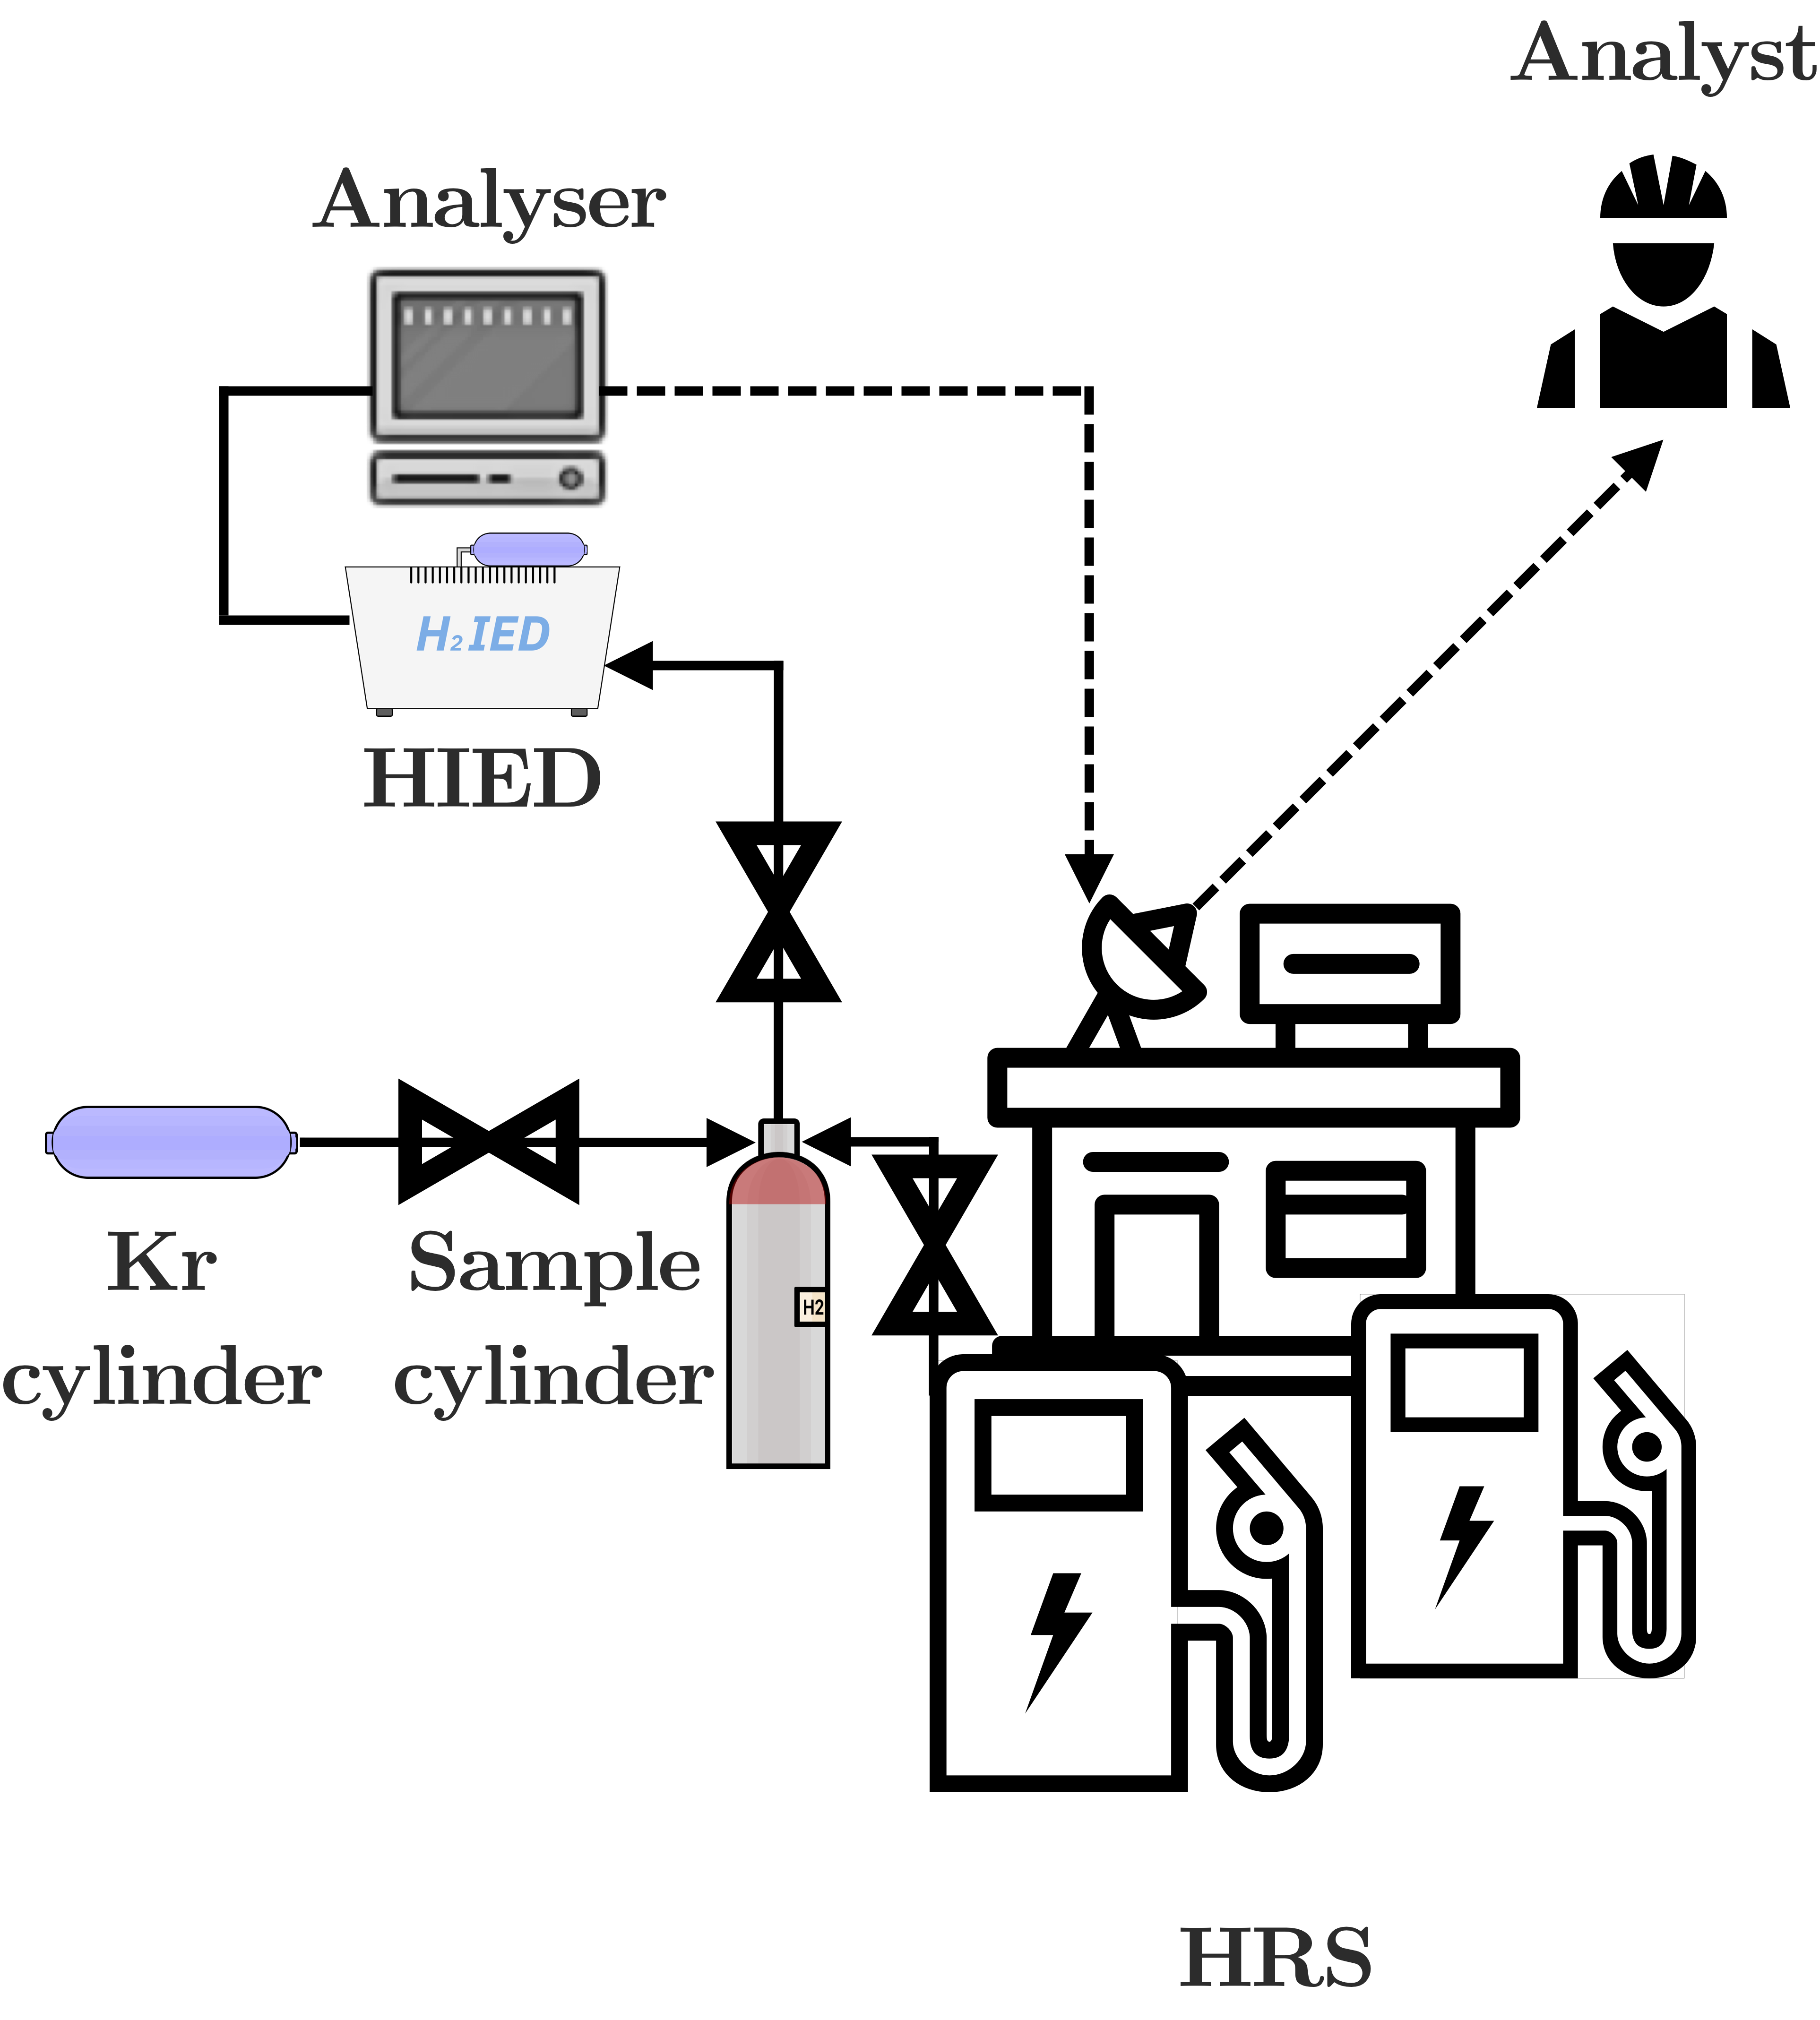
\includegraphics[width=\linewidth, keepaspectratio]{/Users/marc/Thesis/Chapter6/automation.png}
    \caption{Proposed solution for automatic quality assurance of fuel cell hydrogen at HRS's}
    \label{autoprocedure}
\end{figure}

The system could operate automatically through the use of automated valves. When a measurement is required the sample cylinder is evacuated and purged of any remaining gas, before a known mass of krypton defined in chapter 6, is spiked into the empty vessel, measured gravmetrically. The valve connecting the sample cylinder to the HRS is then opened, allowing a certain mass of hydrogen to enter the cylinder to be enriched and tested. Once enough gas has been sampled this valve can be closed, and the sample enriched. Once enrichment is complete the gas automatically passed through a dedicated analyser, tested against a standard, and the results delivered to an analyst off site. This would eliminate the costly and time consuming process of physically acquiring a sample, and transporting it to be tested, allow testing to be performed off site, and allow more flexibability for testing schedules. As the process for performing a hydrogen sample has already been defined \cite{BACQUART20205565} and could be automated with existing technology this could be the next step for impurity enrichment devices. As the market for hydrogen technology increases, modern solutions which greatly improve upon existsing processes such as these will appear increasingly viable.

\subsection{Additional use cases}
There is scope for using the impurity enrichment technique for gases other than hydrogen. Dense ceramic membranes which are permaselective to oxygen are in the research stage, \cite{LIU2005103} and could potentially be inserted into the enrichment device as is to provide this analysis if needed. Another alternative could be to enrich impurities in water to provide a similar analysis. As evidence that pollutants in water are increasing at alarming levels, and are increasingly dangerous to our health, there may be increased scope for water impurity analysis in the future. \cite{marketresearchfirm}

\section{Other hydrogen impurity measurement challenges}
This thesis mainly focused on a technique which is used for off-line analysis of impurities in fuel cell hydrogen. There is still a need for on-line monitoring of impurities at HRS's as stated by ISO 19880-8:2019. In a report performed for the MetroHyve project they concluded that no such devices capable of perfoming on-line sensing exist. Some of the methods used in this thesis, in particular the use of simulations to predict the suitability of a material for a given purpose, could prove useful when researching in this area. 

\section{Closing remarks}
This thesis explored the use of a number of experimental and computational methods to find and test the best membrane for enriching hydrogen impurites to enable testing at a low cost, making the process accessable to a larger number of measurement providers. A commercialised device was designed and has been sold, able to provide purity analysis to within 2\% of the original value. An appropriate membrane composition was found although further work is required to manufacture a low cost membrane. DFT proved to be a useful tool in screening of allows, in particular those resistent to sulphur impurities, however further work must be done to define an appropriate model for the interaction of the alloy surfaces and other impurities. Further work can be done in automation and optimisation of the enrichment device to make it a more commercially viable option.


\bibliographystyle{unsrtnat}
\bibliography{library.bib}

\chapter*{Appendices}
\section*{Uncertainties}
The uncertainties used for gravametric calculation of gas standard is the quadrature sum of the weighing uncertainties before and after the transfer of the component into the vessel.
\begin{table}[H]
    \centering
    \begin{tabular}{@{}cc@{}}
    \toprule
    Balance                   & Standard uncertainty \\ \midrule
    Mettler Toledo XPE26003LC & 20.0 mg                \\
    Satorius 1475 MP8         & 1.4 mg               \\
    Mettler Toledo PR2004     & 0.3 mg               \\
    Mettler Toledo XP2004S    & 0.3 mg               \\
    Mettler Toledo XP205      & 0.1 mg               \\
    Sartorius R160P           & 0.1 mg               \\ \bottomrule
    \end{tabular}
    \caption*{Standard uncertainties (k=1) of the balances used for gravametric preparation of gas standards}
\end{table}

\section*{Metallic Phase Diagrams}
\begin{figure}[H]
  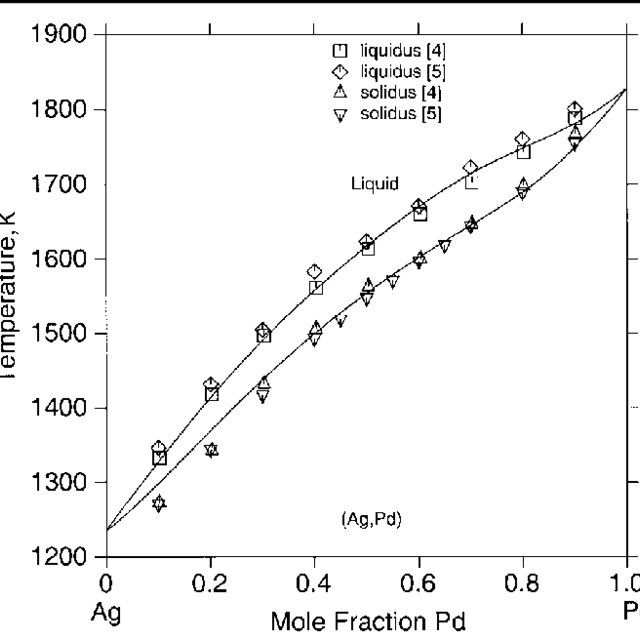
\includegraphics[width=\linewidth]{/Users/marc/Thesis/appendices/PdAg.jpg}
  \caption{The calculated Ag-Pd phase diagram with experimental points \cite{Ghosh1999}}
\end{figure}

\begin{figure}[H]
  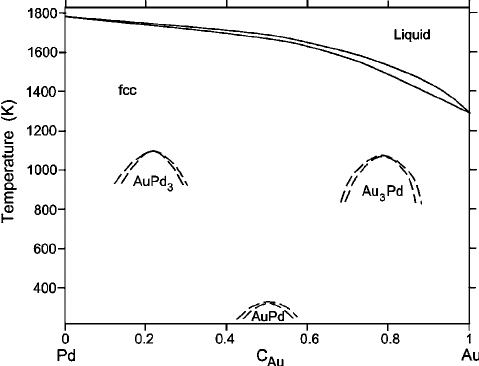
\includegraphics[width=\linewidth]{/Users/marc/Thesis/appendices/AuPd.png}
  \caption{The calculated (dashed) Au-Pd phase diagram with experimental points \cite{Sluiter2006}}
\end{figure}

\begin{figure}[H]
  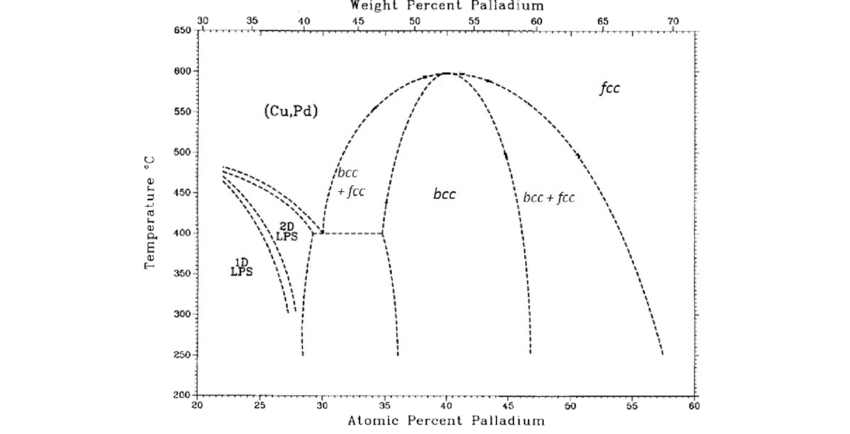
\includegraphics[width=\linewidth]{/Users/marc/Thesis/appendices/CuPd.png}
  \caption{Cu-Pd phase diagram }
\end{figure}

\begin{figure}[H]
  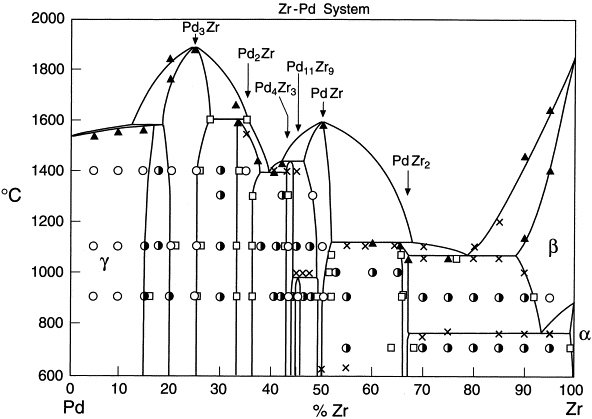
\includegraphics[width=\linewidth]{/Users/marc/Thesis/appendices/ZrPd.png}
  \caption{Zr-Pd phase diagram \cite{WATERSTRAT199963}}
\end{figure}


\section*{Simulation files}
\subsection*{Hydrogen impurities}
\subsubsection*{Ammonia}
\begin{verbatim}
    &CONTROL
    calculation='relax',
    outdir='./tmp/',
    prefix='Ammonia',
    pseudo_dir='/home/mp916/Simulations/qe/qe-6.1/Simulationpdpaper/Pseudo',
    verbosity='high',
    forc_conv_thr = 0.000583,
    tprnfor = .TRUE.
  /
  
  &SYSTEM
    ibrav=0,
    celldm(1)=15.1474115563d0,
    nat=4,
    ntyp=2,
    ecutwfc=30,
    ecutrho=120,
    occupations='smearing',
    degauss=0.005d0,
  /
  &ELECTRONS
    mixing_ndim = 20
    mixing_beta = 0.8
    conv_thr=1d-05,
  /
  &IONS
  /
  ATOMIC_SPECIES
    H 1.007940d0 H.pw91-kjpaw_psl.1.0.0.UPF
    N 14.006700d0 N.pw91-n-kjpaw_psl.1.0.0.UPF
  ATOMIC_POSITIONS {crystal}
     N   0.5042649612d0   0.4816814914d0   0.5185608552d0
     H   0.5858110338d0   0.5710210191d0   0.4807806443d0
     H   0.4526766026d0   0.4289789809d0   0.4165818655d0
     H   0.4141889662d0   0.5407708619d0   0.5834181345d0
  K_POINTS {automatic}
    8 8 8 0 0 0
  CELL_PARAMETERS {alat}
    1.000000000000d0  0.000000000000d0  0.000000000000d0
    0.000000000000d0  0.968552952250d0  0.000000000000d0
    0.000000000000d0  0.000000000000d0  0.994255872719d0
\end{verbatim}
\subsubsection*{Argon}
\begin{verbatim}
    &CONTROL
    calculation='scf',
    outdir='./tmp/',
    prefix='Ar',
    pseudo_dir='/home/mp916/Simulations/qe/qe-6.1/Simulationpdpaper/Pseudo',
    verbosity='high',
    forc_conv_thr = 0.000583,
    tprnfor = .TRUE.
  /
  
  &SYSTEM
    ibrav=0,
    celldm(1)=15.0422199515d0,
    nat=1,
    ntyp=1,
    ecutwfc=30,
    ecutrho=120,
    occupations='smearing',
    smearing='mv',
    degauss=0.005d0,
  /
  
  &ELECTRONS
    mixing_mode = 'local-TF'
    mixing_ndim = 20
    mixing_beta = 0.3
    conv_thr=1d-05,
  /
  
  ATOMIC_SPECIES
    Ar 39.948000d0 Ar.pw91-nl-kjpaw_psl.1.0.0.UPF
  
  ATOMIC_POSITIONS {crystal}
    Ar   0.5000000000d0   0.5000000000d0   0.5000000000d0
  
  K_POINTS {automatic}
    8 8 8 0 0 0
  
  CELL_PARAMETERS {alat}
    1.000000000000d0  0.000000000000d0  0.000000000000d0
    0.000000000000d0  1.000000000000d0  0.000000000000d0
    0.000000000000d0  0.000000000000d0  1.000000000000d0
  
\end{verbatim}

\subsubsection*{Carbon Dioxide}
\begin{verbatim}
    
&CONTROL
calculation='relax',
outdir='./tmp/',
prefix='CO2',
pseudo_dir='/home/mp916/Simulations/qe/qe-6.1/Simulationpdpaper/Pseudo',
verbosity='high',
forc_conv_thr = 0.000583,
tprnfor = .TRUE.
/

&SYSTEM
ibrav=0,
celldm(1)=15.5625245542d0,
nat=3,
ntyp=2,
ecutwfc=30,
ecutrho=120,
occupations='smearing',
smearing='mv',
degauss=0.005d0,
/

&ELECTRONS
mixing_mode = 'local-TF'
mixing_ndim = 20
mixing_beta = 0.3
conv_thr=1d-05,
/

&IONS

/

ATOMIC_SPECIES
C 12.010700d0 C.pw91-n-kjpaw_psl.1.0.0.UPF
O 15.999400d0 O.pw91-n-kjpaw_psl.1.0.0.UPF

ATOMIC_POSITIONS {crystal}
 C   0.5000000007d0   0.5000000008d0   0.4999999998d0
 O   0.4529264144d0   0.4999999999d0   0.3864094181d0
 O   0.5470735856d0   0.4999999992d0   0.6135905819d0

K_POINTS {automatic}
8 8 8 0 0 0

CELL_PARAMETERS {alat}
1.000000000000d0  0.000000000000d0  0.000000000000d0
0.000000000000d0  0.915567068158d0  0.000000000000d0
0.000000000000d0  0.000000000000d0  1.172141239726d0


\end{verbatim}

\subsubsection*{Carbon Monoxide}
\begin{verbatim}
    
&CONTROL
calculation='relax',
outdir='./tmp/',
prefix='CO',
pseudo_dir='/home/mp916/Simulations/qe/qe-6.1/Simulationpdpaper/Pseudo',
verbosity='high',
forc_conv_thr = 0.000583,
tprnfor = .TRUE.
/

&SYSTEM
ibrav=0,
celldm(1)=14.2485349792d0,
nat=2,
ntyp=2,
ecutwfc=30,
ecutrho=120,
occupations='smearing',
smearing='mv',
degauss=0.005d0,
/

&ELECTRONS
mixing_mode = 'local-TF'
mixing_ndim = 20
mixing_beta = 0.3
conv_thr=1d-05,
/

&IONS

/

ATOMIC_SPECIES
C 12.010700d0 C.pw91-n-kjpaw_psl.1.0.0.UPF
O 15.999400d0 O.pw91-n-kjpaw_psl.1.0.0.UPF

ATOMIC_POSITIONS {crystal}
 O   0.5000270812d0   0.5738644516d0   0.5000000000d0
 C   0.4999729188d0   0.4261355484d0   0.5000000000d0

K_POINTS {automatic}
8 8 8 0 0 0

CELL_PARAMETERS {alat}
1.000000000000d0  0.000000000000d0  0.000000000000d0
0.000000000000d0  1.167110986173d0  0.000000000000d0
0.000000000000d0  0.000000000000d0  1.000000000000d0
\end{verbatim}

\subsubsection*{Formaldehyde}
\begin{verbatim}
    
&CONTROL
calculation='relax',
outdir='./tmp/',
prefix='Formaldehyde',
pseudo_dir='/home/mp916/Simulations/qe/qe-6.1/Simulationpdpaper/Pseudo',
verbosity='high',
forc_conv_thr = 0.000583,
tprnfor = .TRUE.
/

&SYSTEM
ibrav=0,
celldm(1)=14.2485349792d0,
nat=4,
ntyp=3,
ecutwfc=30,
ecutrho=120,
occupations='smearing',
smearing='mv',
degauss=0.005d0,
/

&ELECTRONS
mixing_mode = 'local-TF'
mixing_ndim = 20
mixing_beta = 0.3
conv_thr=1d-05,
/

&IONS

/

ATOMIC_SPECIES
C 12.010700d0 C.pw91-n-kjpaw_psl.1.0.0.UPF
O 15.999400d0 O.pw91-n-kjpaw_psl.1.0.0.UPF
H 1.007940d0 H.pw91-kjpaw_psl.1.0.0.UPF

ATOMIC_POSITIONS {crystal}
 H   0.5000032071d0   0.3993778194d0   0.6091900164d0
 C   0.4999967927d0   0.4644674926d0   0.4999863532d0
 H   0.5000032073d0   0.3993419309d0   0.3908099836d0
 O   0.5000031360d0   0.6006580691d0   0.4999707562d0

K_POINTS {automatic}
8 8 8 0 0 0

CELL_PARAMETERS {alat}
1.000000000000d0  0.000000000000d0  0.000000000000d0
0.000000000000d0  1.170692569629d0  0.000000000000d0
0.000000000000d0  0.000000000000d0  1.126681305036d0


\end{verbatim}

\subsubsection*{Formic acid}
\begin{verbatim}
    
&CONTROL
calculation='relax',
outdir='./tmp/',
prefix='Formicacid',
pseudo_dir='/home/mp916/Simulations/qe/qe-6.1/Simulationpdpaper/Pseudo',
verbosity='high',
forc_conv_thr = 0.000583,
tprnfor = .TRUE.
/

&SYSTEM
ibrav=0,
celldm(1)=17.2803095283d0,
nat=5,
ntyp=3,
ecutwfc=30,
ecutrho=120,
occupations='smearing',
smearing='mv',
degauss=0.005d0,
/

&ELECTRONS
mixing_mode = 'local-TF'
mixing_ndim = 20
mixing_beta = 0.3
conv_thr=1d-05,
/

&IONS

/

ATOMIC_SPECIES
C 12.010700d0 C.pw91-n-kjpaw_psl.1.0.0.UPF
O 15.999400d0 O.pw91-n-kjpaw_psl.1.0.0.UPF
H 1.007940d0 H.pw91-kjpaw_psl.1.0.0.UPF

ATOMIC_POSITIONS {crystal}
 H   0.6145158987d0   0.4838354467d0   0.3823127673d0
 C   0.5065122208d0   0.4904111511d0   0.4330303046d0
 O   0.3854841013d0   0.4782033285d0   0.3808877459d0
 O   0.5145431942d0   0.5163076772d0   0.5762053140d0
 H   0.4199060272d0   0.5217966715d0   0.6191122541d0

K_POINTS {automatic}
8 8 8 0 0 0

CELL_PARAMETERS {alat}
1.000000000000d0  0.000000000000d0  0.000000000000d0
0.000000000000d0  0.848121779294d0  0.000000000000d0
0.000000000000d0  0.000000000000d0  1.013821874194d0


\end{verbatim}

\subsubsection*{Hydrogen}
\begin{verbatim}
    
&CONTROL
calculation='relax',
outdir='./tmp/',
prefix='Hydrogen',
pseudo_dir='/home/mp916/Simulations/qe/qe-6.1/Simulationpdpaper/Pseudo',
verbosity='high',
forc_conv_thr = 0.000583,
tprnfor = .TRUE.
/

&SYSTEM
ibrav=0,
celldm(1)=12.6119438239d0,
nat=2,
ntyp=1,
ecutwfc=30,
ecutrho=120,
occupations='smearing',
smearing='mv',
degauss=0.005d0,
/

&ELECTRONS
mixing_mode = 'local-TF'
mixing_ndim = 20
mixing_beta = 0.3
conv_thr=1d-05,
/

&IONS


/

ATOMIC_SPECIES
H 1.007940d0 H.pw91-kjpaw_psl.1.0.0.UPF

ATOMIC_POSITIONS {crystal}
 H   0.5025437140d0   0.5504756643d0   0.4980656210d0
 H   0.4974562860d0   0.4495243357d0   0.5019343790d0

K_POINTS {automatic}
8 8 8 0 0 0

CELL_PARAMETERS {alat}
1.000000000000d0  0.000000000000d0  0.000000000000d0
-0.500000000000d0  0.866025403784d0  0.000000000000d0
0.000000000000d0  0.000000000000d0  3.858856497911d0
\end{verbatim}

\subsubsection*{Helium}
\begin{verbatim}
    
&CONTROL
calculation='scf',
outdir='./tmp/',
prefix='He',
pseudo_dir='/home/mp916/Simulations/qe/qe-6.1/Simulationpdpaper/Pseudo',
verbosity='high',
forc_conv_thr = 0.000583,
tprnfor = .TRUE.
/

&SYSTEM
ibrav=0,
celldm(1)=14.8532473391d0,
nat=1,
ntyp=1,
ecutwfc=30,
ecutrho=120,
occupations='smearing',
smearing='mv',
degauss=0.005d0,
/

&ELECTRONS
mixing_mode = 'local-TF'
mixing_ndim = 20
mixing_beta = 0.3
conv_thr=1d-05,
/

&IONS

/

ATOMIC_SPECIES
He 4.002600d0 He.pw91-kjpaw_psl.1.0.0.UPF

ATOMIC_POSITIONS {crystal}
He   0.5000000000d0   0.5000000000d0   0.5000000000d0

K_POINTS {automatic}
8 8 8 0 0 0

CELL_PARAMETERS {alat}
1.000000000000d0  0.000000000000d0  0.000000000000d0
0.000000000000d0  1.000000000000d0  0.000000000000d0
0.000000000000d0  0.000000000000d0  1.000000000000d0


\end{verbatim}

\subsubsection*{Hydrogen Sulphide}
\begin{verbatim}
    
&CONTROL
calculation='relax',
outdir='./tmp/',
prefix='h2s',
pseudo_dir='/home/mp916/Simulations/qe/qe-6.1/Simulationpdpaper/Pseudo',
verbosity='high',
forc_conv_thr = 0.000583,
tprnfor = .TRUE.
/

&SYSTEM
ibrav=0,
celldm(1)=16.0398870722d0,
nat=3,
ntyp=2,
ecutwfc=30,
ecutrho=120,
occupations='smearing',
smearing='mv',
degauss=0.005d0,
/

&ELECTRONS
mixing_mode = 'local-TF'
mixing_ndim = 20
mixing_beta = 0.3
conv_thr=1d-05,
/

&IONS

/

ATOMIC_SPECIES
H 1.007940d0 H.pw91-kjpaw_psl.1.0.0.UPF
S 32.065000d0 S.pw91-nl-kjpaw_psl.1.0.0.UPF

ATOMIC_POSITIONS {crystal}
 H   0.5676219636d0   0.4950645124d0   0.3911640247d0
 S   0.4323780364d0   0.5049354876d0   0.4708913462d0
 H   0.5069112201d0   0.4960181453d0   0.6088359753d0

K_POINTS {automatic}
8 8 8 0 0 0

CELL_PARAMETERS {alat}
1.000000000000d0  0.000000000000d0  0.000000000000d0
0.000000000000d0  0.947225998108d0  0.000000000000d0
0.000000000000d0  0.000000000000d0  1.003132863700d0


\end{verbatim}

\subsubsection*{Methane}
\begin{verbatim}
    
&CONTROL
calculation='relax',
outdir='./tmp/',
prefix='ch4',
pseudo_dir='/home/mp916/Simulations/qe/qe-6.1/Simulationpdpaper/Pseudo',
verbosity='high',
forc_conv_thr = 0.000583,
tprnfor = .TRUE.
/

&SYSTEM
ibrav=0,
celldm(1)=15.5988312226d0,
nat=5,
ntyp=2,
ecutwfc=30,
ecutrho=120,
occupations='smearing',
smearing='mv',
degauss=0.005d0,
/

&ELECTRONS
mixing_mode = 'local-TF'
mixing_ndim = 20
mixing_beta = 0.3
conv_thr=1d-05,
/

&IONS

/

ATOMIC_SPECIES
C 12.010700d0 C.pw91-n-kjpaw_psl.1.0.0.UPF
H 1.007940d0 H.pw91-kjpaw_psl.1.0.0.UPF

ATOMIC_POSITIONS {crystal}
 H   0.5977973834d0   0.5255779311d0   0.4030437573d0
 C   0.4844150120d0   0.5064005724d0   0.4672387946d0
 H   0.4022026166d0   0.6045463354d0   0.4423372459d0
 H   0.4299497513d0   0.3954536646d0   0.4266264303d0
 H   0.5076890964d0   0.4999969626d0   0.5969562427d0

K_POINTS {automatic}
8 8 8 0 0 0

CELL_PARAMETERS {alat}
1.000000000000d0  0.000000000000d0  0.000000000000d0
0.000000000000d0  1.017066353498d0  0.000000000000d0
0.000000000000d0  0.000000000000d0  0.997913028772d0


\end{verbatim}

\subsubsection*{Nitrogen}
\begin{verbatim}
    
&CONTROL
calculation='relax',
outdir='./tmp/',
prefix='n2',
pseudo_dir='/home/mp916/Simulations/qe/qe-6.1/Simulationpdpaper/Pseudo',
verbosity='high',
forc_conv_thr = 0.000583,
tprnfor = .TRUE.
/

&SYSTEM
ibrav=0,
celldm(1)=14.1735975053d0,
nat=2,
ntyp=1,
ecutwfc=30,
ecutrho=120,
occupations='smearing',
smearing='mv',
degauss=0.005d0,
/

&ELECTRONS
mixing_mode = 'local-TF'
mixing_ndim = 20
mixing_beta = 0.3
conv_thr=1d-05,
/

&IONS

/

ATOMIC_SPECIES
N 14.006700d0 N.pw91-n-kjpaw_psl.1.0.0.UPF

ATOMIC_POSITIONS {crystal}
 N   0.5000229854d0   0.5638317643d0   0.5000000000d0
 N   0.4999770146d0   0.4361682357d0   0.5000000000d0

K_POINTS {automatic}
8 8 8 0 0 0

CELL_PARAMETERS {alat}
1.000000000000d0  0.000000000000d0  0.000000000000d0
0.000000000000d0  1.146293961020d0  0.000000000000d0
0.000000000000d0  0.000000000000d0  0.999954029241d0


\end{verbatim}

\subsubsection*{Oxygen}
\begin{verbatim}
    
&CONTROL
calculation='relax',
outdir='./tmp/',
prefix='O2',
pseudo_dir='/home/mp916/Simulations/qe/qe-6.1/Simulationpdpaper/Pseudo',
verbosity='high',
forc_conv_thr = 0.000583,
tprnfor = .TRUE.
/

&SYSTEM
ibrav=0,
celldm(1)=14.0980751846d0,
nat=2,
ntyp=1,
ecutwfc=30,
ecutrho=120,
occupations='smearing',
smearing='mv',
degauss=0.005d0,
/

&ELECTRONS
mixing_mode = 'local-TF'
mixing_ndim = 20
mixing_beta = 0.3
conv_thr=1d-05,
/

&IONS

/

ATOMIC_SPECIES
O 15.999400d0 O.pw91-n-kjpaw_psl.1.0.0.UPF

ATOMIC_POSITIONS {crystal}
 O   0.5000254749d0   0.5697808506d0   0.5000000000d0
 O   0.4999745251d0   0.4302191494d0   0.5000000000d0

K_POINTS {automatic}
8 8 8 0 0 0

CELL_PARAMETERS {alat}
1.000000000000d0  0.000000000000d0  0.000000000000d0
0.000000000000d0  1.162139169543d0  0.000000000000d0
0.000000000000d0  0.000000000000d0  0.999949050114d0


\end{verbatim}
\subsubsection*{Water}
\begin{verbatim}

&CONTROL
calculation='relax',
outdir='./tmp/',
prefix='Water',
pseudo_dir='/home/mp916/Simulations/qe/qe-6.1/Simulationpdpaper/Pseudo',
verbosity='high',
forc_conv_thr = 0.000583,
tprnfor = .TRUE.
/

&SYSTEM
ibrav=0,
celldm(1)=14.8665566802d0,
nat=3,
ntyp=2,
ecutwfc=30,
ecutrho=120,
occupations='smearing',
smearing='mv',
degauss=0.005d0,
/

&ELECTRONS
mixing_mode = 'local-TF'
mixing_ndim = 20
mixing_beta = 0.3
conv_thr=1d-05,
/

&IONS

/

ATOMIC_SPECIES
O 15.999400d0 O.pw91-n-kjpaw_psl.1.0.0.UPF
H 1.007940d0 H.pw91-kjpaw_psl.1.0.0.UPF

ATOMIC_POSITIONS {crystal}
 H   0.5519282150d0   0.4962140751d0   0.4124172883d0
 O   0.4480717850d0   0.5037859249d0   0.4724366744d0
 H   0.4747052991d0   0.4993010724d0   0.5875827117d0

K_POINTS {automatic}
8 8 8 0 0 0

CELL_PARAMETERS {alat}
1.000000000000d0  0.000000000000d0  0.000000000000d0
0.000000000000d0  0.948259720965d0  0.000000000000d0
0.000000000000d0  0.000000000000d0  1.023268717357d0
\end{verbatim}
\subsection*{Palladium system}
\subsubsection*{Example system adsorbing Hydrogen on the surface of PdAg }
\begin{verbatim}
    &CONTROL
  calculation='scf',
  outdir='./tmp/',
  prefix='pdh2sfcc',
  pseudo_dir='/media/mp916/0A6296CF6296BF3F/MembraneDFTscript/Simulationpdpaper/Pseudo',
  verbosity='high',
  forc_conv_thr = 0.000583,
  tprnfor = .TRUE.
/

&SYSTEM
  ibrav=0,
  celldm(1)=10.3967346064d0,
  nat=23,
  ntyp=4,
  ecutwfc=30,
  ecutrho=120,
  occupations='smearing',
  degauss=0.005d0,
/

&ELECTRONS
  mixing_mode = 'local-TF'
  mixing_ndim = 21
  mixing_beta = 0.1
  conv_thr=1d-03,
/

&IONS

/

ATOMIC_SPECIES
  H  1.007940d0  H.pw91-kjpaw_psl.1.0.0.UPF
  Pd 106.420000d0 Pd.pw91-n-kjpaw_psl.1.0.0.UPF
  S 32.065000d0 S.pw91-nl-kjpaw_psl.1.0.0.UPF
    Ag 107.868000d0 Ag.pw91-n-kjpaw_psl.1.0.0.UPF


ATOMIC_POSITIONS {crystal}
  Pd   0.1666669970d0   0.3333339940d0   0.0991198960d0 0 0 0
    Pd   0.6666666670d0   0.3333333330d0   0.0991197760d0 0 0 0
    Pd   0.1666669970d0   0.8333330030d0   0.0991198960d0 0 0 0
    Ag   0.6666660060d0   0.8333330030d0   0.0991198960d0 0 0 0
    Pd   0.0000000000d0   0.0000000000d0   0.2084872330d0 0 0 0
    Ag   0.4999994680d0  -0.0000010630d0   0.2084882210d0 0 0 0
    Pd   0.0000010630d0   0.5000005320d0   0.2084882210d0 0 0 0
    Ag   0.4999994680d0   0.5000005320d0   0.2084882210d0 0 0 0
    Pd   0.3333331390d0   0.1666665700d0   0.3175525410d0 1 1 1 
    Pd   0.8333334300d0   0.1666665700d0   0.3175525410d0 1 1 1
    Pd   0.3333333330d0   0.6666666670d0   0.3175526140d0 1 1 1
    Pd   0.8333334300d0   0.6666668610d0   0.3175525410d0 1 1 1 
    Pd   0.1666668260d0   0.3333336520d0   0.4262792350d0 1 1 1
    Ag   0.6666666670d0   0.3333333330d0   0.4262800040d0 1 1 1
    Pd   0.1666668260d0   0.8333331740d0   0.4262792350d0 1 1 1
    Pd   0.6666663480d0   0.8333331740d0   0.4262792350d0 1 1 1
    Pd   0.0000000000d0   0.0000000000d0   0.5354872520d0 1 1 1
    Ag   0.4999992870d0  -0.0000014260d0   0.5354874210d0 1 1 1
    Pd   0.0000014260d0   0.5000007130d0   0.5354874210d0 1 1 1
    Pd   0.4999987651d0   0.5000007130d0   0.5354874210d0 1 1 1 
   S   0.8333338900d0   0.1666664227d0   0.5595108834d0 1 1 1
   H   0.8415731417d0   0.1791808477d0   0.6225635207d0 1 1 1
   H   1.1011049065d0   0.3005523705d0   0.5788091707d0 1 1 1

K_POINTS {automatic}
  4 4 4 1 1 0

CELL_PARAMETERS {alat}
  1.000000000000d0  0.000000000000d0  0.000000000000d0
  -0.500000000000d0  0.866025403784d0  0.000000000000d0
  0.000000000000d0  0.000000000000d0  3.858856497911d0
\end{verbatim}

\section*{EDS mapping of membranes}
\begin{figure}[H]
  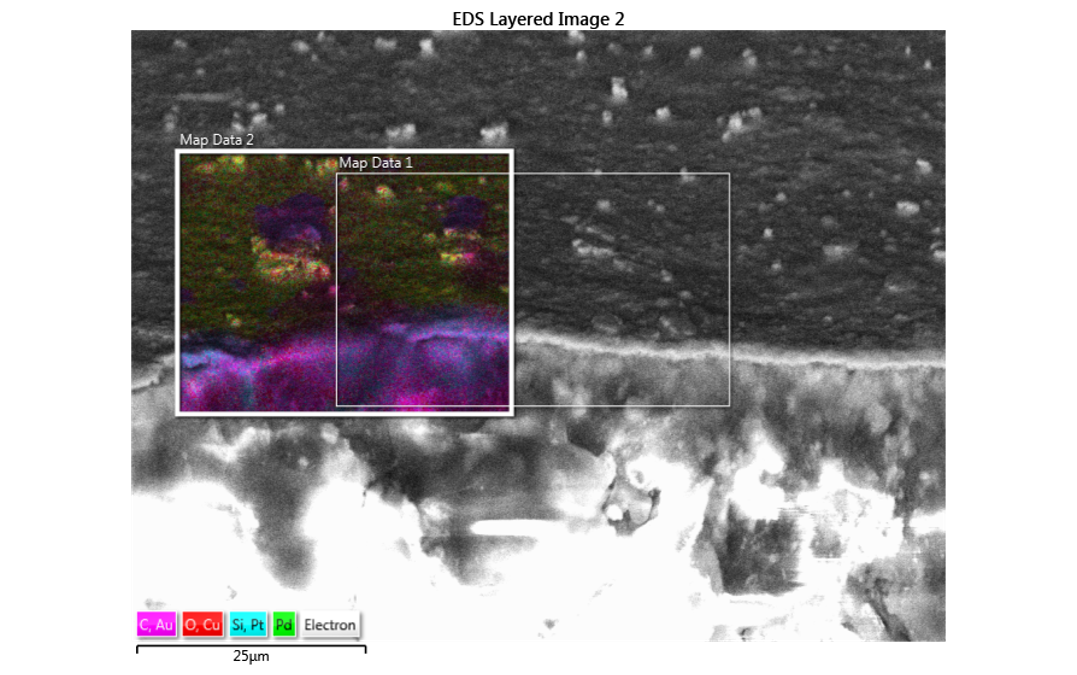
\includegraphics[width=\linewidth]{/Users/marc/Thesis/appendices/edspdcuau.png}
\end{figure}

\begin{figure}[H]
  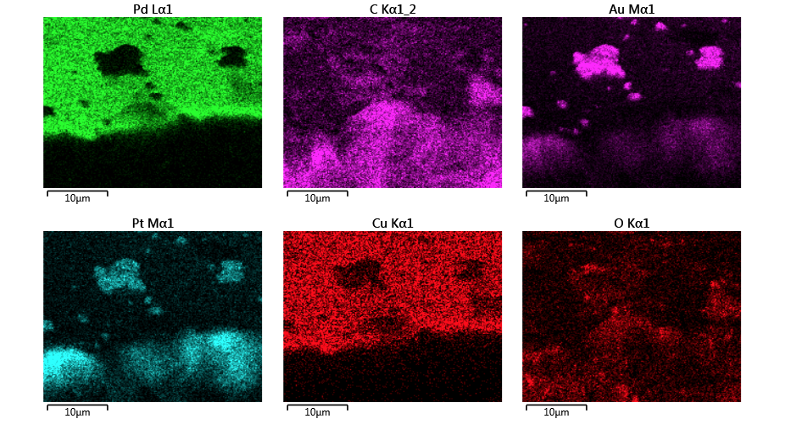
\includegraphics[width=\linewidth]{/Users/marc/Thesis/appendices/edspdcuau1.png}
\end{figure}

\begin{figure}[H]
  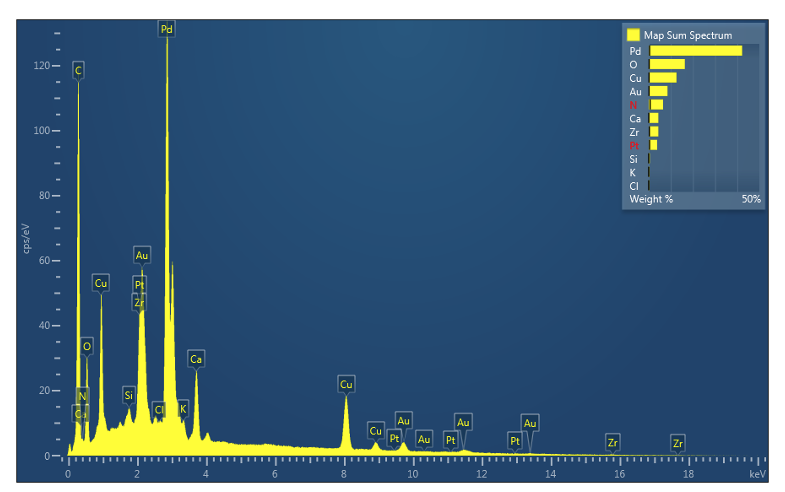
\includegraphics[width=\linewidth]{/Users/marc/Thesis/appendices/edspdcuau2.png}
  \caption{PdCuAu EDS spectra}
\end{figure}


\begin{figure}[H]
  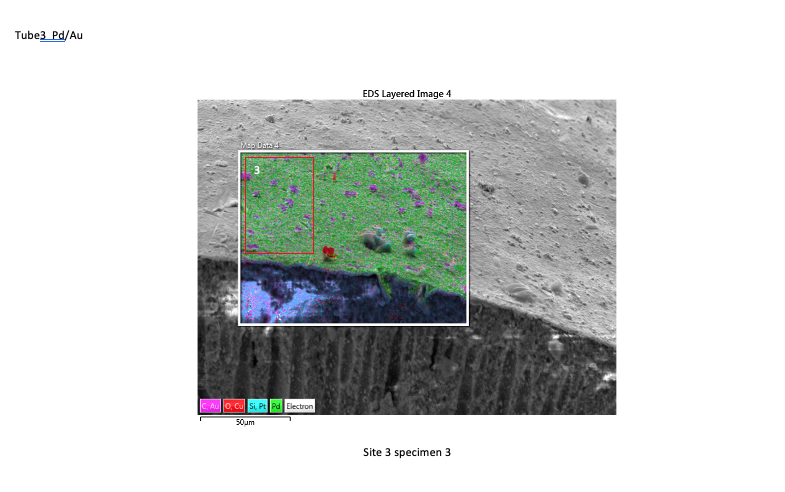
\includegraphics[width=\linewidth]{/Users/marc/Thesis/appendices/edspdau.png}
\end{figure}
\begin{figure}[H]
  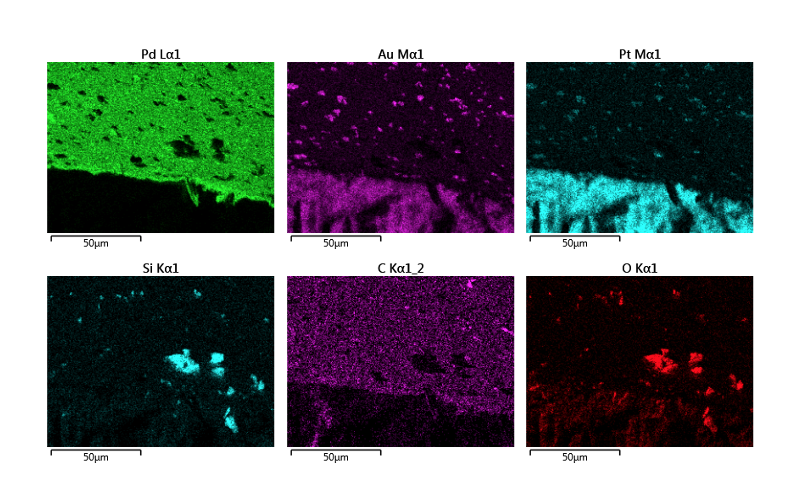
\includegraphics[width=\linewidth]{/Users/marc/Thesis/appendices/edspdau1.png}
\end{figure}

\begin{figure}[H]
  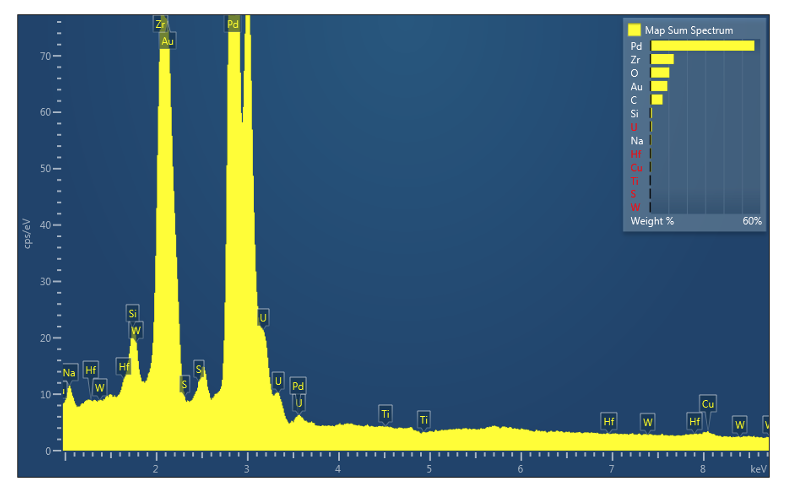
\includegraphics[width=\linewidth]{/Users/marc/Thesis/appendices/edspdau2.png}
  \caption{PdAu EDS spectra}
\end{figure}

\begin{figure}[H]
  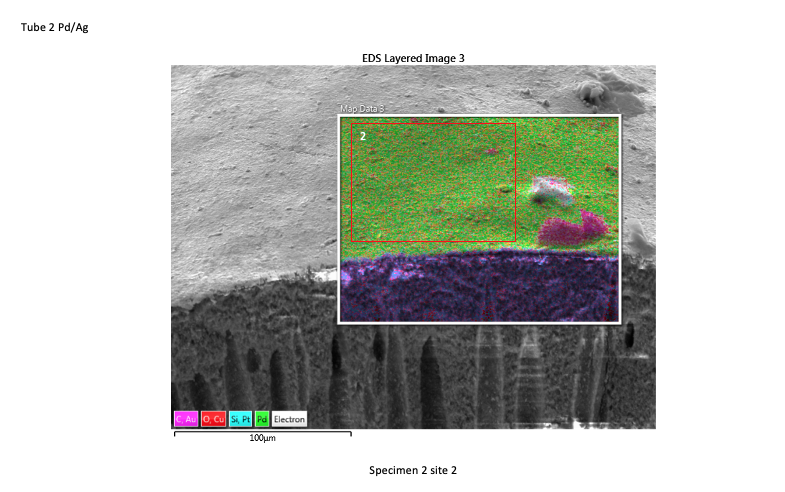
\includegraphics[width=\linewidth]{/Users/marc/Thesis/appendices/edspdag.png}
\end{figure}

\begin{figure}[H]
  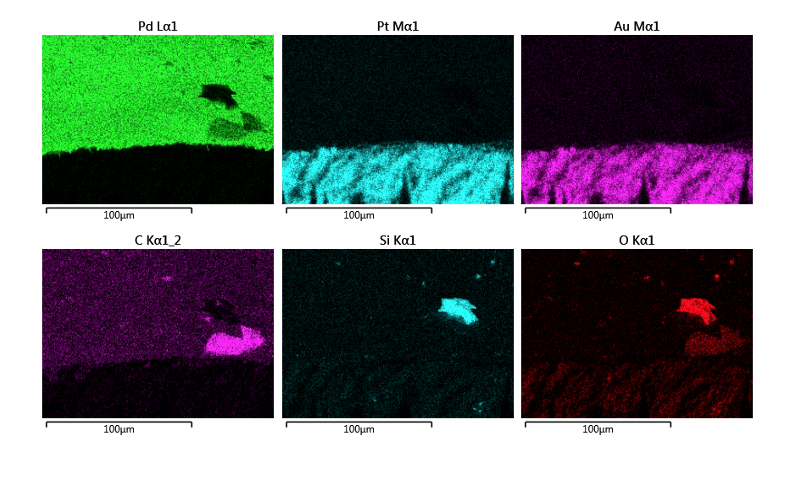
\includegraphics[width=\linewidth]{/Users/marc/Thesis/appendices/edspdag1.png}
  \caption{PdAg EDS spectra}
\end{figure}

\begin{figure}[H]
  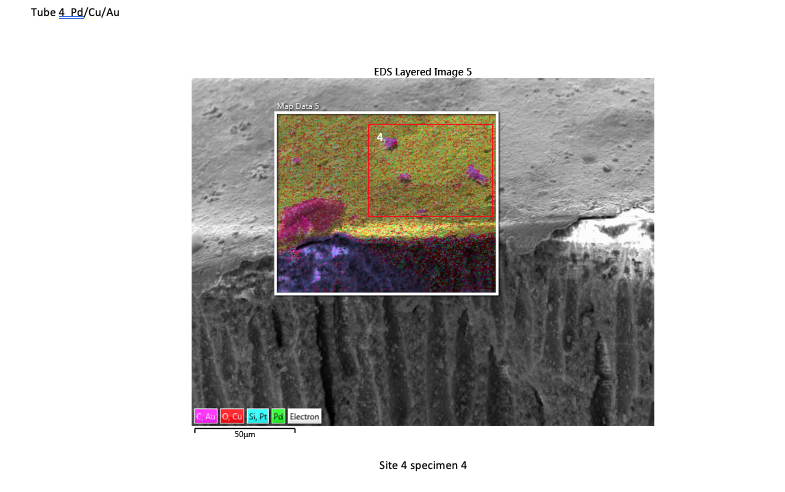
\includegraphics[width=\linewidth]{/Users/marc/Thesis/appendices/edspdcu.png}
\end{figure}
\begin{figure}[H]
  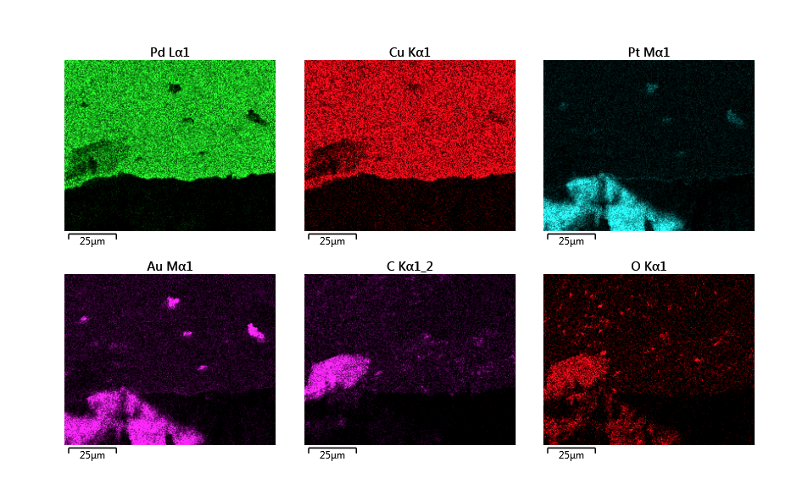
\includegraphics[width=\linewidth]{/Users/marc/Thesis/appendices/edspdcu1.png}
\end{figure}

\begin{figure}[H]
  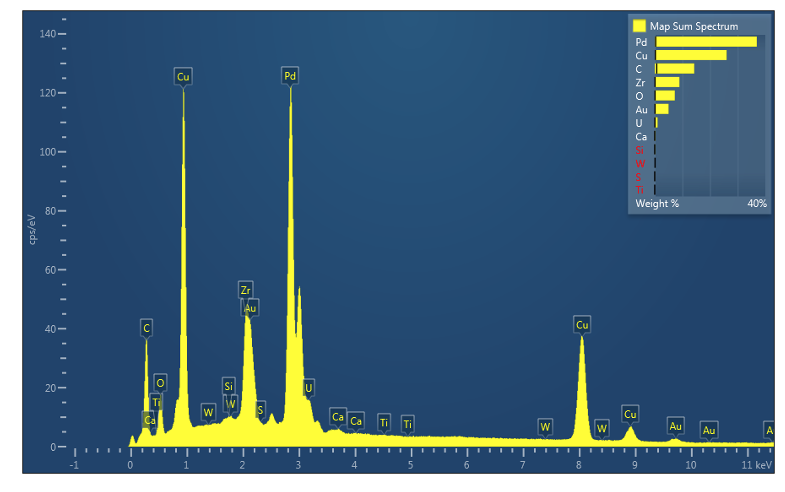
\includegraphics[width=\linewidth]{/Users/marc/Thesis/appendices/edspdcu2.png}
  \caption{PdCu EDS spectra}
\end{figure}

\begin{figure}[H]
  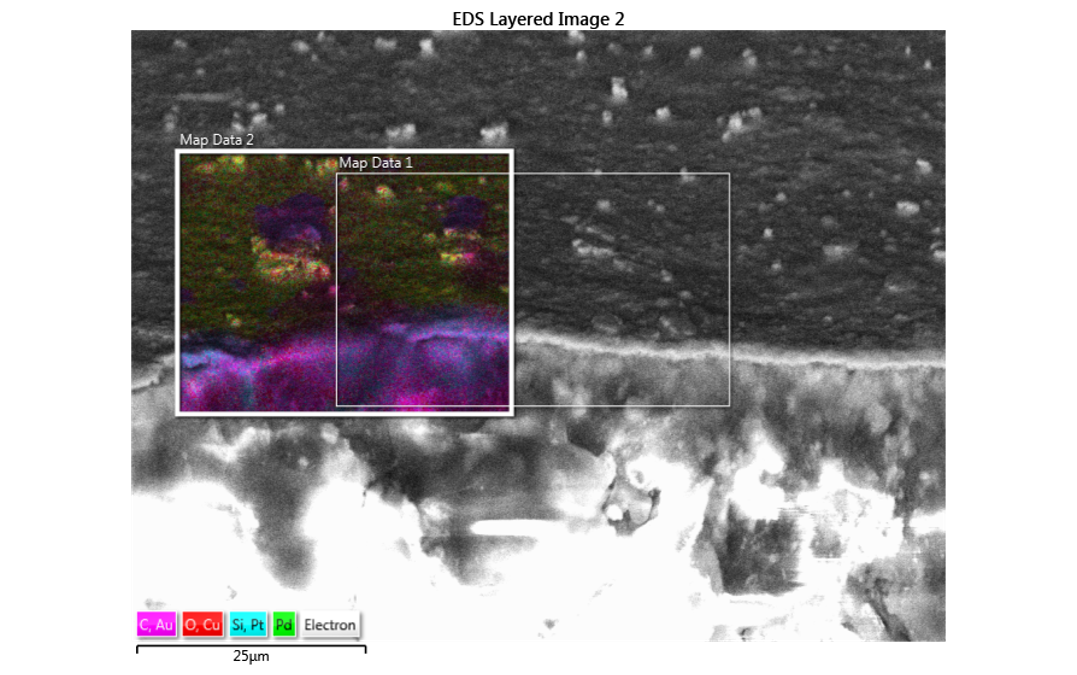
\includegraphics[width=\linewidth]{/Users/marc/Thesis/appendices/edspdcuau.png}
\end{figure}
\begin{figure}[H]
  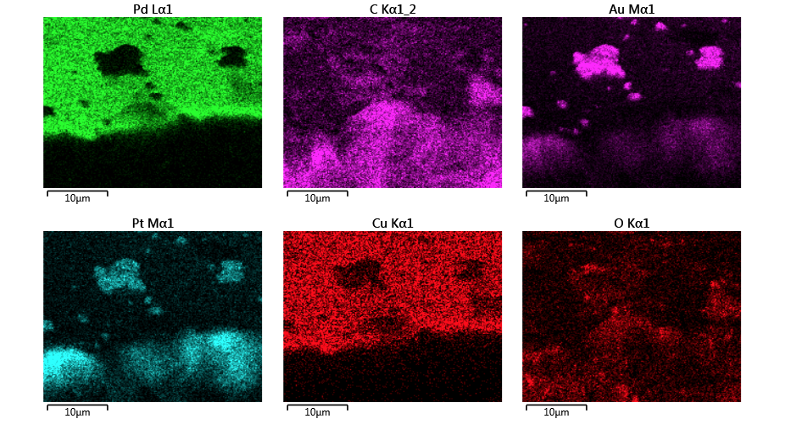
\includegraphics[width=\linewidth]{/Users/marc/Thesis/appendices/edspdcuau1.png}
\end{figure}

\begin{figure}[H]
  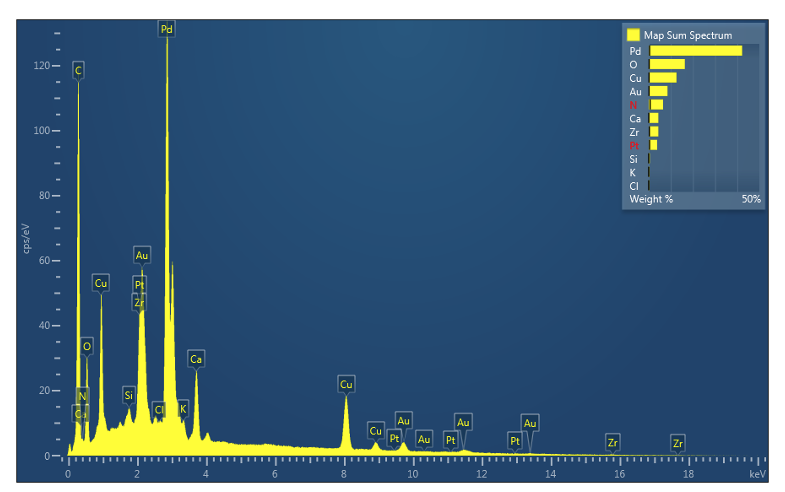
\includegraphics[width=\linewidth]{/Users/marc/Thesis/appendices/edspdcuau2.png}
  \caption{PdCuAu EDS spectra}
\end{figure}

\begin{figure}[H]
  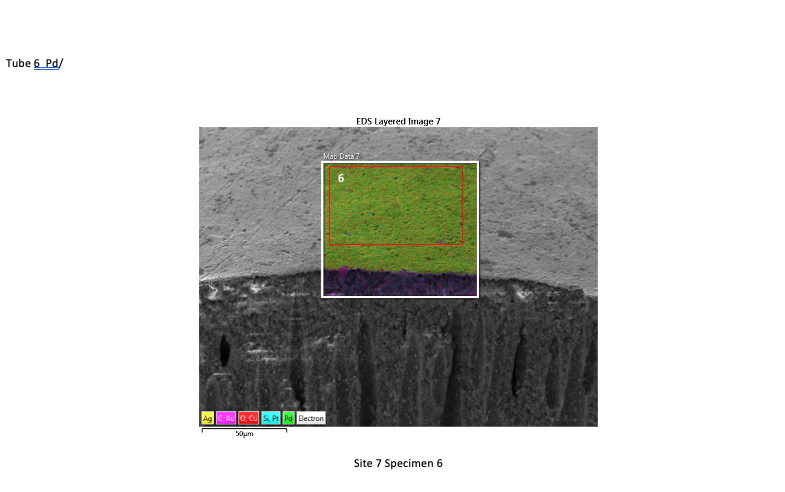
\includegraphics[width=\linewidth]{/Users/marc/Thesis/appendices/edspd.png}
\end{figure}
\begin{figure}[H]
  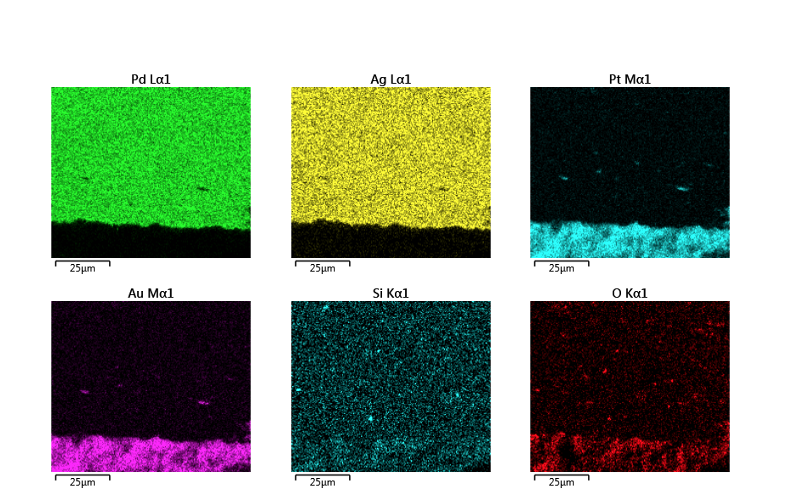
\includegraphics[width=\linewidth]{/Users/marc/Thesis/appendices/edspd1.png}
\end{figure}

\begin{figure}[H]
  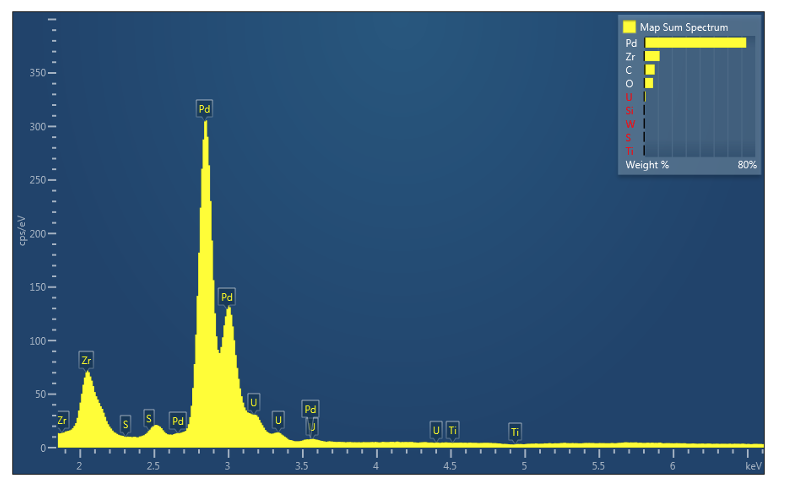
\includegraphics[width=\linewidth]{/Users/marc/Thesis/appendices/edspd2.png}
  \caption{PdCuAu EDS spectra}
\end{figure}

\section*{Pictures of commercial enrichment device}

\begin{figure}[H]
    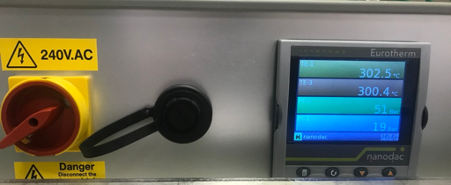
\includegraphics[width=\linewidth]{/Users/marc/Thesis/appendices/Picture1.png}
    \caption{Enrichment device control panel}
  \end{figure}

  \begin{figure}[H]
    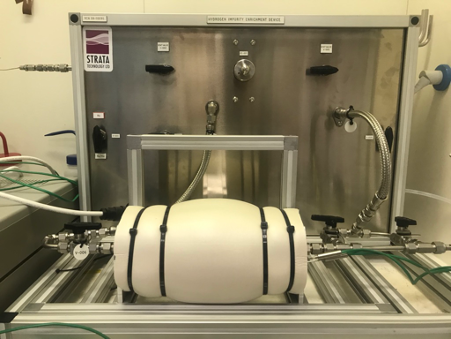
\includegraphics[width=\linewidth]{/Users/marc/Thesis/appendices/Picture2.png}
    \caption{Enrichment device chassis layout}
  \end{figure}

  \begin{figure}[H]
    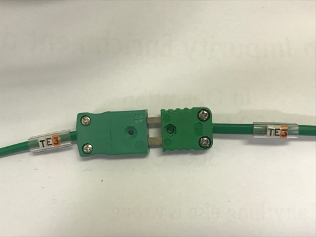
\includegraphics[width=\linewidth]{/Users/marc/Thesis/appendices/Picture3.png}
    \caption{Example of connecting thermocouples using TE3}
  \end{figure}

  \begin{figure}[H]
    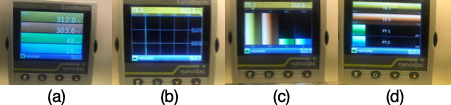
\includegraphics[width=\linewidth]{/Users/marc/Thesis/appendices/Picture4.png}
    \caption{Information based views on eurotherm control panel (a) System Summary (b) Vertical trend over time (c) Vertical bar chart (d) Horizontal bar chart}
  \end{figure}

  \begin{figure}[H]
    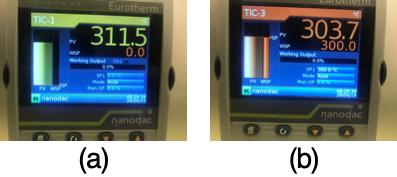
\includegraphics[width=\linewidth]{/Users/marc/Thesis/appendices/Picture5.png}
    \caption{Temperature control views}
  \end{figure}

  \begin{figure}[H]
    \includegraphics[width=\linewidth]{/Users/marc/Thesis/appendices/Picture6.png}
    \caption{Heating switch}
  \end{figure}

  \begin{figure}[H]
    \includegraphics[width=\linewidth]{/Users/marc/Thesis/appendices/Picture7.png}
    \caption{Disconnected transportable unit}
  \end{figure}

  \bibliographystyle{unsrtnat}
  \bibliography{library.bib}

\chapter*{List of Publications and Presentations}

\section*{Publications}
\begin{enumerate}
    \item \textbf{M. Plunkett}, K.Li, A. Murugan; Review of membrane technologies for hydrogen impurity enrichment (To be resubmitted)
    \item \textbf{M. Plunkett}, A. Morris, S. Nayebossardi, T. Bacquart, B. Wang,  S. Spencer, K. Mingard, K. Li, A. Murugan ; Determining impurity resistant palladium alloy membrane compositions for enrichment of hydrogen fuel samples with low level contaminants (In final preparation)
    \item \textbf{M. Plunkett}, N. Moore, T. Bacquart, K.Li, A. Murugan; Analysing low level impurities in hydrogen refuelling station hydrogen using hydrogen impurity enrichment; (In preparation)

\end{enumerate}

\section*{Oral Presentations}
\begin{enumerate}
    \item \textbf{M. Plunkett}, A. Murugan, K. Li; A hydrogen impurity enrichment device using Pd-Alloy membranes to support the hydrogen economy. Presented at International Conference for Membrane and Electromembrane Processes 2018, 13th – 16th May 2018, Prague, Czech Republic.
    \item \textbf{M. Plunkett}, A. Murugan, K. Li; A hydrogen impurity enrichment device using Pd-Alloy membranes to support the hydrogen economy. Presented at 15th International Conference on Inorganic Membranes, 18th – 22nd June 2018, Dresden, Germany. 
    \item \textbf{M. Plunkett}; Determining impurity resistant palladium alloy membrane compositions for enrichment of hydrogen fuel samples with low level ISO 14687-2 contaminants. Presented at 2nd bi-annual Gas and Particle Metrology symposium, 14th August, 2018, Teddington, United Kingdom 
    \item \textbf{M. Plunkett}; Developing suitable palladium alloy membranes for enrichment of hydrogen fuel samples to satisfy growing analytical demand. Presented at H2FC Research Conference University of Birmingham, 14th August, 2018, Birmingham, United Kingdom 
    \item \textbf{M. Plunkett}; Hydrogen Quality Assurance Work Package 2, Task 2.4: Optimisation of impurity enrichment devices. EMPIR MetroHyVe M39 meeting, 25th August, 2020, Online 
\end{enumerate}


\end{document}